\documentclass[8pt]{article}
\usepackage[utf8]{inputenc}
\usepackage[doublespacing]{setspace}
\usepackage{german}
\usepackage{enumitem}
\usepackage{hyperref}
\usepackage{tikz}
\usepackage{marvosym,graphicx}
\usepackage{capt-of}

\newcommand{\STOPP}
{\begin{center}
\tikz[baseline=-1ex]{
 \draw[line width=1.2pt,scale=0.6,baseline=-0.5ex]
  (22.5:1)--(3*22.5:1)--(5*22.5:1)--(7*22.5:1)--(9*22.5:1)--(11*22.5:1)--(13*22.5:1)--(15*22.5:1)--cycle;
 \fill[scale=0.53,baseline=-0.5ex]
  (22.5:1)--(3*22.5:1)--(5*22.5:1)--(7*22.5:1)--(9*22.5:1)--(11*22.5:1)--(13*22.5:1)--(15*22.5:1)--cycle;
\node [white,font=\small\bfseries\sffamily] {STOP};}
\end{center}}


\newcommand{\STOP}{
\begin{center}
\scalebox{2}{\raisebox{-1.7ex}{\Huge\Stopsign}} 
\end{center}}


\newcommand\Warning{%
 \makebox[1.4em][c]{%
 \makebox[0pt][c]{\raisebox{.1em}{\small!}}%
 \makebox[0pt][c]{\color{red}\Large$\bigtriangleup$}}}%
 
\begin{document}

Das vorliegende Dokument soll eine Ergänzung zu den altbekannten und zum Teil frei verfügbaren Hilfsmitteln \textbf{Moltrecht} als auch \textbf{Lichtblicke} von DL9HCG sein. Ich verwende dabei den offiziellen Fragenkatalog der Bundesnetzagentur mit allen verfügbaren Fragen in exakt der gleichen Reihenfolge, wie sie auch im regulären Fragenkatalog verwendet wird. \textbf{Auch in diesem Dokument stellt Frage A immer die richtige Frageantwort dar.} Im Gegensatz zu der Dokumentation von DL9HCG beschreibe ich aber nicht, wie die einzelnen Werte in den Taschenrechner einzugeben sind, sondern verweise auf die jeweiligen Formeln und stelle weitere Links zu den jeweiligen Fragen bereit, die vielleicht im Rahmen der Bearbeitung der Fragen hilfreich sind.

Ziel soll es sein, die Antworten nicht stumpf auswendig zu lernen, sondern auch zu verstehen, was sich hinter den einzelnen Fragestellungen verbirgt. Als begleitendes Material empfehle ich die Lichtblicke von DL9HCG, den Molrecht-Onlinekurs (auf den Seiten des DARC zu finden) sowie das Lizenzkochbuch von DL2ANM. Die Moltrecht-Bücher können hilfreich sein - ich habe sie allerdings für meine Prüfung fast nicht verwendet und mich stattdessen nur auf den Onlinekurs konzentriert. Für einzelne Teile dieses Dokuments greife ich auch textuell auf diese Dokumente zurück.

Im Anhang befinden sich zusätzliche Links und Verweise auf Ausbildungsunterlagen, die Dich auf Deiner Reise zur Amateurfunklizenz der Klasse A unterstützen werden. Ich empfehle, wenigstens einmal alle Technikfragen komplett durchzuarbeiten.

55+73,
Jörg
DF1JSL
 
\section {Prüfungsfragen im Prüfungsteil „Technische Kenntnisse“ der Klasse A}
\subsection {Allgemeine mathematische Grundkenntnisse und Größen}
\subsubsection {Allgemeine mathematische Grundkenntnisse}
Der hierzu erforderliche Prüfungsstoff ist in den Abschnitten 1.1.2 bis 1.12 enthalten.\\
\subsubsection{Größen und Einheiten}
Der hierzu erforderliche Prüfungsstoff ist in den Abschnitten 1.1.2 bis 1.12 enthalten.


\paragraph*{TA101 Welche Einheit wird für die elektrische Feldstärke verwendet?}
\begin{enumerate}[nolistsep,label=\Alph*]
\item Volt pro Meter ($\frac{V}{m}$)
\item Watt pro Quadratmeter ($\frac{W}{m^{2}}$)
\item Ampere pro Meter ($\frac{A}{m}$)
\item Henry pro Meter ($\frac{H}{m}$)
\end{enumerate}
Die \textbf{elektrische Feldstärke} $E$ bildet sich ausgehend von stromdurchflossenen Materialien aus. Mit zunehmender Entfernung schwächt sich das Feld ab. Wird an die Platten eines Kondensators eine Wechselspannung angelegt, dann wechselt das Feld zwischen den Platten entsprechend die Richtung und Stärke.\\
Definition: $E$ = $\frac{U}{d}$ mit 
\begin{enumerate}
\item $U$ = Spannung [Volt]
\item $d$ = Abstand [Meter]
\end{enumerate}
Die Einheit der elektrischen Feldstärke $E$ ist somit $\frac{V}{m}$.


\paragraph*{TA102 Welche Einheit wird für die magnetische Feldstärke verwendet?}
\begin{enumerate}[nolistsep,label=\Alph*]
\item Ampere pro Meter ($\frac{A}{m}$)
\item Tesla (T)
\item Amperemeter (Am)
\item Henry pro Meter ($\frac{H}{m}$)
\end{enumerate}
Die \textbf{magnetische Feldstärke} $H$ bildet sich bei dem Anlegen einer Wechselspannung an einen Leiter; es wird ein Magnetfeld aufgebaut. Mit Anlegen der Wechselspannung wechselt das Magnetfeld Richtung und Stärke entsprechend der Umladungen. Mit jedem Umladen des Magnetfeldes breitet sich ein neuer Schlauch um den Leiter aus,der sich - größer und schwächer werdend - vom Leiter entfernt, bis er endlich ganz abklingt.\\
Definition: $H$ = $\frac{I * n}{l_{m}}$ mit
\begin{enumerate}
\item $H$ = magn. Feldstärke in Ampere pro Meter (A/m)
\item $I$ =Strom in Ampere ( A )
\item $N$ = Windungszahl
\item $l_{m}$ = mittlere Feldlinienlänge in Meter


\paragraph*{TA103 In welcher Einheit wird die Impedanz angegeben?}
\begin{enumerate}[nolistsep,label=\Alph*]
\item Ohm
\item Farad
\item Siemens
\item Henry
\end{enumerate}



\paragraph*{TA104 Die Einheit Siemens wird verwendet für die Angabe}
\begin{enumerate}[nolistsep,label=\Alph*]
\item des Leitwertes eines Widerstands.
\item des Ohmschen Widerstands.
\item der Impedanz einer Leitung.
\item der magnetischen Feldstärke.
\end{enumerate}



\paragraph*{TA105 Wenn [s] für Sekunde steht, gilt für die Einheit der Frequenz}
\begin{enumerate}[nolistsep,label=\Alph*]
\item $Hz$ = $\frac{1}{s}$ 
\item $Hz$ = $s$
\item $Hz$ = $s^{2}$
\item $Hz$ = $\frac{1}{s^{2}}$
\end{enumerate}



\paragraph*{TA106 Welche der nachfolgenden Antworten enthält nur Basiseinheiten nach dem internationalen Einheitensystem?}
\begin{enumerate}[nolistsep,label=\Alph*]
\item Meter, Kelvin, Sekunde, Ampere
\item Radiant, Meter, Volt, Watt
\item Farad, Henry, Ohm, Sekunde
\item Grad, Hertz, Ohm, Tesla
\end{enumerate}



\paragraph*{TA107 Einem Spannungsverhältnis von 15 entsprechen}
\begin{enumerate}[nolistsep,label=\Alph*]
\item 23,5 dB.
\item 52 dB.
\item 47 dB.
\item 11,7 dB.
\end{enumerate}



\paragraph*{TA108 Einer Leistungsverstärkung von 40 entsprechen}
\begin{enumerate}[nolistsep,label=\Alph*]
\item 16 dB.
\item 60 dB.
\item 32 dB.
\item 24 dB.
\end{enumerate}



\paragraph*{TA109 Wie groß ist der Unterschied zwischen S4 und S7 in dB?}
\begin{enumerate}[nolistsep,label=\Alph*]
\item 18 dB
\item 9 dB
\item 28 dB
\item 3 dB
\end{enumerate}



\paragraph*{TA110 Der Pegelwert 120 $dB\mu$ $\frac{V}{m}$ entspricht einer elektrischen Feldstärke von}
\begin{enumerate}[nolistsep,label=\Alph*]
\item 1 $\frac{V}{m}$.
\item 10 $\frac{V}{m}$.
\item 1000 $\frac{V}{m}$.
\item 1000 $\frac{kV}{m}$.
\end{enumerate}



\paragraph*{TA111 100 mW entspricht}
\begin{enumerate}[nolistsep,label=\Alph*]
\item $10^{-1}$ W.
\item 0,001 W.
\item 0,01 W.
\item $10^{-2}$ W.
\end{enumerate}



\paragraph*{TA112 Ein Sender mit 1 Watt Ausgangsleistung ist an eine Endstufe mit einer Verstärkung von 10 dB angeschlossen. Wie groß ist der Ausgangspegel der Endstufe?}
\begin{enumerate}[nolistsep,label=\Alph*]
\item 40 dBm
\item 30 dBm
\item 20 dBm
\item 10 dBm
\end{enumerate}



\paragraph*{TA113 Der Ausgangspegel eines Senders beträgt 20 dBW. Dies entspricht einer Ausgangsleistung von}
\begin{enumerate}[nolistsep,label=\Alph*]
\item 102 W.
\item 100,5 W.
\item 1020 W.
\item 101 W.
\end{enumerate}



\paragraph*{TA114 Die Periodendauer von 50 $\mu$s entspricht einer Frequenz von}
\begin{enumerate}[nolistsep,label=\Alph*]
\item 20 kHz.
\item 2 MHz.
\item 200 kHz.
\item 20 MHz.
\end{enumerate}



\paragraph*{TA115 Die zweite Harmonische der Frequenz 3,730 MHz befindet sich auf}
\begin{enumerate}[nolistsep,label=\Alph*]
\item 7,460 MHz.
\item 1,865 MHz.
\item 11,190 MHz.
\item 14,920 MHz.
\end{enumerate}



\paragraph*{TA116 Die zweite ungeradzahlige Harmonische der Frequenz 144,690 MHz ist}
\begin{enumerate}[nolistsep,label=\Alph*]
\item 434,070 MHz.
\item 289,380 MHz.
\item 145,000 MHz.
\item 723,450 MHz.
\end{enumerate}



\paragraph*{TA117 Eine Genauigkeit von 1 ppm entspricht}
\begin{enumerate}[nolistsep,label=\Alph*]
\item 0,0001 \%.
\item 0,001 \%.
\item 0,01 \%.
\item 0,1 \%.
\end{enumerate}



\paragraph*{TA118 Die digitale Anzeige eines Senders hat eine Anzeigegenauigkeit von 10 ppm. Sie zeigt die Sendefrequenz von 14,25 MHz an. In welchen Grenzen kann sich die tatsächliche Frequenz bewegen?}
\begin{enumerate}[nolistsep,label=\Alph*]
\item Zwischen 14,2498575 und 14,2501425 MHz
\item Zwischen 14,24998575 und 14,25001425 MHz
\item Zwischen 14,249998575 und 14,250001425 MHz
\item Zwischen 14,248575 und 14,251425 MHz
\end{enumerate}



\paragraph*{TA119 Die Ausbreitungsgeschwindigkeit freier elektromagnetischer Wellen beträgt etwa}
\begin{enumerate}[nolistsep,label=\Alph*]
\item 300000 $\frac{km}{s}$.
\item 3000.000 $\frac{km}{s}$.
\item 30000 $\frac{km}{s}$.
\item 3000 $\frac{km}{s}$. 
\end{enumerate}



\paragraph*{TA120 Welche Frequenz entspricht einer Wellenlänge von 30 mm im Freiraum?}
\begin{enumerate}[nolistsep,label=\Alph*]
\item 10 GHz
\item 100 MHz
\item 1 MHz
\item 100 kHz
\end{enumerate}



\paragraph*{TA121 Eine Wellenlänge von 10 cm im Freiraum entspricht einer Frequenz von}
\begin{enumerate}[nolistsep,label=\Alph*]
\item 3 GHz.
\item 1,9 GHz.
\item 3 MHz.
\item 10 GHz.
\end{enumerate}



\paragraph*{TA122 Welcher Wellenlänge $\Lambda$ entspricht die Frequenz} f = 22 MHz?
\begin{enumerate}[nolistsep,label=\Alph*]
\item $\Lambda$ = 13,64 m
\item $\Lambda$ = 14,33 m
\item $\Lambda$ = 12,93 m
\item $\Lambda$ = 136,3 m
\end{enumerate}



\paragraph*{TA123 Eine Wellenlänge von 2,06 m entspricht einer Frequenz von}
\begin{enumerate}[nolistsep,label=\Alph*]
\item 145,631 MHz.
\item 150,247 MHz.
\item 148,927 MHz.
\item 135,754 MHz.
\end{enumerate}



\paragraph*{TA124 Eine Wellenlänge von 69 cm entspricht einer Frequenz von}
\begin{enumerate}[nolistsep,label=\Alph*]
\item 434,783 MHz.
\item 430,162 MHz.
\item 435,574 MHz.
\item 440,317 MHz.
\end{enumerate}



\paragraph*{TA125 Der Verkürzungsfaktor ist}
\begin{enumerate}[nolistsep,label=\Alph*]
\item das Verhältnis der Ausbreitungsgeschwindigkeit entlang einer Leitung zur Ausbreitungsgeschwindigkeit im Vakuum.
\item das Verhältnis von Durchmesser zur Länge eines Leiters.
\item das Verhältnis des Wellen- bzw. des Strahlungswiderstandes zum Feldwellenwiderstand des freien Raumes.
\item die Wurzel aus dem Verhältnis von Induktivität zur Kapazität einer Leitung.
\end{enumerate}


\pagebreak
\subsection{Elektrizitäts-, Elektromagnetismus- und Funktheorie}
\subsubsection{Leiter, Halbleiter und Isolator}


\paragraph*{TB101 Der spezifische Widerstand eines Drahtes entspricht dem Widerstand des Drahtes}
\begin{enumerate}[nolistsep,label=\Alph*]
\item bei einer Länge von 1000 mm und einem Querschnitt von 1 $mm^{2}$. 
\item bei einer Länge von 100 mm und einem Querschnitt von 1 $mm^{2}$.
\item bei einer Länge von 1 m und einem Querschnitt von 0,1 $mm^{2}$.
\item bei einer Länge von 100 mm und einem Querschnitt von 0,1 $mm^{2}$.
\end{enumerate}



\paragraph*{TB102 Welchen Widerstand hat eine Kupferdrahtwicklung, wenn der verwendete Draht eine Länge von 1,8 m und einen Durchmesser von 0,2 mm hat?}
\begin{enumerate}[nolistsep,label=\Alph*]
\item 1 $\Omega$
\item 56 $\Omega$
\item 0,05 $\Omega$
\item 5,6 $\Omega$
\end{enumerate}



\paragraph*{TB103 Zwischen den Enden eines Kupferdrahtes mit einem Querschnitt von 0,5 $mm^{2}$ messen Sie einen Widerstand von 1,5 $\Omega$. Wie lang ist der Draht?}
\begin{enumerate}[nolistsep,label=\Alph*]
\item 42,1 m
\item 25,3 m
\item 4,2 m
\item 168,5 m
\end{enumerate}



\paragraph*{TB104 Der Temperaturkoeffizient für den Widerstand von metallischen Leitern ist}
\begin{enumerate}[nolistsep,label=\Alph*]
\item positiv.
\item negativ.
\item logarithmisch.
\item exponentiell.
\end{enumerate}



\paragraph*{TB105 Welche Gruppe von Materialien enthält nur Nichtleiter (Isolatoren)?}
\begin{enumerate}[nolistsep,label=\Alph*]
\item Epoxyd, Polyethylen (PE), Polystyrol (PS)
\item Pertinax, Polyvinylchlorid (PVC), Graphit
\item Polyethylen (PE), Messing, Konstantan
\item Teflon, Pertinax, Bronze
\end{enumerate}



\paragraph*{TB106 Was versteht man unter Halbleitermaterialien?}
\begin{enumerate}[nolistsep,label=\Alph*]
\item Einige Stoffe (z.B. Silizium, Germanium) sind in reinem Zustand bei Zimmertemperatur gute Isolatoren. Durch geringfügige Zusätze von geeigneten anderen Stoffen oder bei hohen Temperaturen werden sie jedoch zu Leitern.
\item Einige Stoffe (z.B. Silizium, Germanium) sind in reinem Zustand bei Zimmertemperatur gute Leiter. Durch geringfügige Zusätze von geeigneten anderen Stoffen oder bei hohen Temperaturen nimmt jedoch ihre Leitfähigkeit ab.
\item Einige Stoffe wie z.B. Indium oder Magnesium sind in reinem Zustand gute Isolatoren. Durch geringfügige Zusätze von Silizium, Germanium oder geeigneten anderen Stoffen werden sie jedoch zu Leitern.
\item Einige Stoffe (z.B. Silizium, Germanium) sind in trockenem Zustand gute Elektrolyten. Durch geringfügige Zusätze von Wismut oder Tellur kann man daraus entweder N-leitendes- oder P-leitendes Material für Anoden bzw. Katoden von Halbleiterbauelementen herstellen.
\end{enumerate}



\paragraph*{TB107 P-leitendes Halbleitermaterial ist gekennzeichnet durch}
\begin{enumerate}[nolistsep,label=\Alph*]
\item bewegliche Elektronenlücken.
\item das Fehlen von Dotierungsatomen.
\item das Fehlen von Atomen im Gitter des Halbleiterkristalls.
\item Überschuss an freien Elektronen.
\end{enumerate}



\paragraph*{TB108 Was versteht man unter Dotierung zu P-leitendem Halbleitermaterial bei Halbleiterwerkstoffen?}
\begin{enumerate}[nolistsep,label=\Alph*]
\item Zugabe von dreiwertigen Stoffen zum vierwertigen Halbleitergrundstoff 
\item Zugabe von fünfwertigen Stoffen zum vierwertigen Halbleitergrundstoff
\item Zugabe von Germaniumatomen zum Siliziumgrundwerkstoff
\item Zugabe von Siliziumatomen zum Germaniumgrundwerkstoff
\end{enumerate}



\paragraph*{TB109 N-leitendes Halbleitermaterial ist gekennzeichnet durch}
\begin{enumerate}[nolistsep,label=\Alph*]
\item das Vorhandensein frei beweglicher Elektronen.
\item das Fehlen von Dotierungsatomen.
\item das Fehlen von Atomen im Gitter des Halbleiterkristalls.
\item das Vorhandensein beweglicher Elektronenlücken.
\end{enumerate}



\paragraph*{TB110 Was versteht man unter Dotierung zu N-leitendem Halbleitermaterial bei Halbleiterwerkstoffen?}
\begin{enumerate}[nolistsep,label=\Alph*]
\item Zugabe von fünfwertigen Stoffen zum vierwertigen Halbleitergrundstoff
\item Zugabe von dreiwertigen Stoffen zum vierwertigen Halbleitergrundstoff
\item Zugabe von Germaniumatomen zum Siliziumgrundwerkstoff
\item Zugabe von Siliziumatomen zum Germaniumgrundwerkstoff
\end{enumerate}



\paragraph*{TB111 Das folgende Bild zeigt den prinzipiellen Aufbau einer Halbleiterdiode. Wie entsteht die Sperrschicht?}
\begin{center}
	\begin{minipage}{\linewidth}
		\centering
		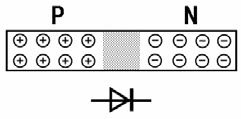
\includegraphics[scale=0.7]{pics/tb111_a.jpg}

	\end{minipage}
\end{center}
\begin{enumerate}[nolistsep,label=\Alph*]
\item An der Grenzschicht wandern Elektronen aus dem N-Teil in den P-Teil. Dadurch wird auf der N-Seite der Elektronenüberschuss teilweise abgebaut, auf der P-Seite der Elektronenmangel teilweise neutralisiert. Es bildet sich auf beiden Seiten der Grenzfläche eine isolierende Schicht.
\item An der Grenzschicht wandern Elektronen aus dem P-Teil in den N-Teil. Dadurch wird auf der P-Seite der Elektronenüberschuss teilweise abgebaut, auf der N-Seite der Elektronenmangel teilweise neutralisiert. Es bildet sich auf beiden Seiten der Grenzfläche eine isolierende Schicht.
\item An der Grenzschicht wandern Atome aus der Grenzschicht in den N- und P-Teil. Dadurch wird auf beiden Seiten der Atommangel abgebaut. Es bildet sich auf der P-Seite eine leitende Schicht. 
\item An der Grenzschicht wandern Atome aus dem N-Teil in den P-Teil. Dadurch wird auf der N-Seite der Atommangel abgebaut, auf der P-Seite der Atommangel vergrößert. Es bildet sich auf der N-Seite eine leitende Schicht.
\end{enumerate}



\paragraph*{TB112 In einer Halbleiterdiode erweitert sich die Verarmungszone,}
\begin{center}
	\begin{minipage}{\linewidth}
		\centering
		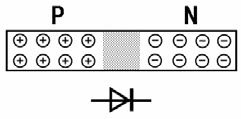
\includegraphics[scale=0.7]{pics/tb112_a.jpg}
	\end{minipage}
\end{center}
\begin{enumerate}[nolistsep,label=\Alph*]
\item wenn man an die Katode (N-Gebiet) eine positive und an die Anode (P-Gebiet) eine negative Spannung anlegt.
\item wenn man an die Katode (P-Gebiet) eine positive und an die Anode (N-Gebiet) eine negative Spannung anlegt.
\item wenn man an die Katode (P-Gebiet) eine negative und an die Anode (N-Gebiet) eine positive Spannung anlegt.
\item wenn man an die Katode (N-Gebiet) eine negative und an die Anode (P-Gebiet) eine positive Spannung anlegt.
\end{enumerate}


\pagebreak
\subsubsection{Strom- und Spannungsquellen}

\paragraph*{TB201 Ein Sonnenkollektor besteht aus vier parallel geschalteten Reihen von je 30 Solarzellen mit je Zelle 0,6 V Leerlaufspannung und 1 A Kurzschlussstrom. Welche Leerlaufspannung und welchen Kurzschlussstrom liefert der Kollektor? In welcher Zeile sind beide Werte richtig angegeben?}
\begin{center}
	\begin{minipage}{\linewidth}
		\centering
		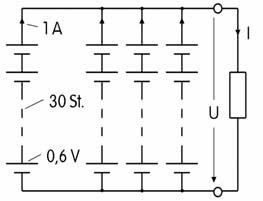
\includegraphics[scale=0.7]{pics/tb201_a.jpg}
	\end{minipage}
\end{center}
\begin{enumerate}[nolistsep,label=\Alph*]
\item Leerlaufspannung: 18 V, Kurzschlussstrom: 4 A
\item Leerlaufspannung: 18 V, Kurzschlussstrom: 30 A
\item Leerlaufspannung: 2,4 V, Kurzschlussstrom: 4 A
\item Leerlaufspannung: 2,4 V, Kurzschlussstrom: 30 A
\end{enumerate}



\paragraph*{TB202 Die Leerlaufspannung einer Gleichspannungsquelle beträgt 13,5 V. Wenn die Spannungsquelle einen Strom von 0,9 A abgibt, sinkt die Klemmenspannung auf 12,4 V. Wie groß ist der Innenwiderstand der Spannungsquelle?}
\begin{enumerate}[nolistsep,label=\Alph*]
\item 1,22 $\Omega$
\item 0,82 $\Omega$
\item 12,15 $\Omega$
\item 1,1 $\Omega$
\end{enumerate}



\paragraph*{TB203 Die Leerlaufspannung einer Gleichspannungsquelle beträgt 13,5 V. Wenn die Spannungsquelle einen Strom von 2 A abgibt, sinkt die Klemmenspannung auf 13 V. Wie groß ist der Innenwiderstand der Spannungsquelle?}
\begin{enumerate}[nolistsep,label=\Alph*]
\item 0,25 $\Omega$
\item 6,75 $\Omega$
\item 13 $\Omega$
\item 0,5 $\Omega$
\end{enumerate}



\paragraph*{TB204 Die Leerlaufspannung einer Gleichspannungsquelle beträgt 13,5 V. Wenn die Spannungsquelle einen Strom von 1 A abgibt, sinkt die Klemmenspannung auf 12,5 V. Wie groß ist der Wirkungsgrad?}
\begin{enumerate}[nolistsep,label=\Alph*]
\item 92,6 \%
\item 100 \%
\item 7,5 \%
\item 13,5 \%
\end{enumerate}



\paragraph*{TB205 Die Leerlaufspannung einer Gleichspannungsquelle beträgt 13,5 V. Wenn die Spannungsquelle einen Strom von 2 A abgibt, sinkt die Klemmenspannung auf 13 V. Wie groß ist der Wirkungsgrad?}
\begin{enumerate}[nolistsep,label=\Alph*]
\item 96,3 \%
\item 100 \%
\item 3,7 \%
\item 27 \%
\end{enumerate}



\paragraph*{TB206 Die Leerlaufspannung einer Spannungsquelle beträgt 5,0 V. Schließt man einen Belastungswiderstand mit 1,2  an, so geht die Klemmenspannung der Spannungsquelle auf 4,8 V zurück. Wie hoch ist der Innenwiderstand der Spannungsquelle?}
\begin{enumerate}[nolistsep,label=\Alph*]
\item 0,05 $\Omega$
\item 8,2 $\Omega$
\item 0,2 $\Omega$
\item 0,25 $\Omega$
\end{enumerate}



\paragraph*{TB207 In welchem Zusammenhang müssen Innenwiderstand $R_{I}$ und Lastwiderstand $R_{L}$ stehen, damit Leistungsanpassung vorliegt?}
\begin{enumerate}[nolistsep,label=\Alph*]
\item $R_{L}$ = $R_{I}$
\item $R_{L}$ $\gg$ $R_{I}$
\item $R_{L}$ $\ll$ $R_{I}$
\item $R_{L}$ = $\frac{1}{R_{i}}$
\end{enumerate}



\paragraph*{TB208 In welchem Zusammenhang müssen Innenwiderstand $R_{I}$ und Lastwiderstand $R_{L}$ stehen, damit Stromanpassung vorliegt?}
\begin{enumerate}[nolistsep,label=\Alph*]
\item $R_{L}$ $\ll$ $R_{I}$
\item $R_{L}$ $\gg$ $R_{I}$
\item $R_{L}$ = $R_{I}$
\item $R_{L}$ = $\frac{1}{R_{i}}$
\end{enumerate} 



\paragraph*{TB209 In welchem Zusammenhang müssen Innenwiderstand $R_{I}$ und Lastwiderstand $R_{L}$ stehen, damit Spannungsanpassung vorliegt?}
\begin{enumerate}[nolistsep,label=\Alph*]
\item $R_{L}$ $\gg$ $R_{I}$
\item $R_{L}$ $\ll$ $R_{I}$
\item $R_{L}$ = $R_{I}$
\item $R_{L}$ = $\frac{1}{R_{i}}$
\end{enumerate}



\paragraph*{TB210 Welche Eigenschaften sollten Strom- und Spannungsquellen aufweisen?}
\begin{enumerate}[nolistsep,label=\Alph*]
\item Spannungsquellen sollten einen möglichst niedrigen Innenwiderstand und Stromquellen einen möglichst hohen Innenwiderstand haben.
\item Strom- und Spannungsquellen sollten einen möglichst niedrigen Innenwiderstand haben. 
\item Strom- und Spannungsquellen sollten einen möglichst hohen Innenwiderstand haben.
\item Spannungsquellen sollten einen möglichst hohen Innenwiderstand und Stromquellen einen möglichst niedrigen Innenwiderstand haben.
\end{enumerate}


\pagebreak
\subsubsection{Elektrisches Feld}


\paragraph*{TB301 An den Metallbelägen eines Wickelkondensators mit 0,15 mm starkem Kunststoff-Dielektrikum liegt eine Spannung von 300 V. Wie hoch ist die elektrische Feldstärke zwischen den Metallbelägen?}
\begin{center}
	\begin{minipage}{\linewidth}
		\centering
		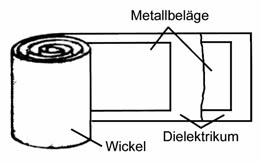
\includegraphics[scale=0.7]{pics/tb301_a.jpg}
	\end{minipage}
\end{center}
\begin{enumerate}[nolistsep,label=\Alph*]
\item 2000 $\frac{kV}{m}$
\item 200 $\frac{V}{m}$
\item 2000 $\frac{V}{m}$
\item 200 $\frac{kV}{m}$
\end{enumerate}



\paragraph*{TB302 Eine Blockbatterie hat eine Klemmenspannung von 9 V (EMK). Wie groß ist die elektrische Feldstärke zwischen den beiden Polen der Batterie bei einem Polabstand von 0,6 cm?}
\begin{enumerate}[nolistsep,label=\Alph*]
\item Zirka 1500 $\frac{V}{m}$
\item Zirka 150 $\frac{V}{m}$
\item Zirka 15 $\frac{V}{m}$
\item Zirka 5,4 $\frac{V}{m}$
\end{enumerate}



\paragraph*{TB303 Die elektrische Feldstärke um einen einzelnen Leiter ist proportional} 
\begin{enumerate}[nolistsep,label=\Alph*]
\item zur Spannung am Leiter.
\item zum Strom durch den Leiter.
\item zum Querschnitt des Leiters.
\item zur Länge des Leiters.
\end{enumerate}



\paragraph*{TB304 Ein HF-Abklatschkondensator am Anodenkreis einer Senderendstufe hat eine 0,15 mm starke PTFE-Folie als Dielektrikum. Die Durchschlagsfestigkeit von PTFE beträgt ca. 400 $\frac{kV}{cm}$. Wie groß wäre die maximale Spannung, die an den Kondensator angelegt werden kann, ohne dass die Folie durchschlagen wird?}
\begin{enumerate}[nolistsep,label=\Alph*]
\item 6 kV
\item 60 kV
\item 600 V
\item 2,6 kV
\end{enumerate}



\paragraph*{TB305 Wie nennt man das Feld zwischen zwei parallelen Kondensatorplatten bei Anschluss einer Gleichspannung?}
\begin{center}
	\begin{minipage}{\linewidth}
		\centering
		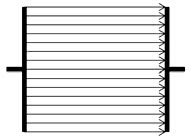
\includegraphics[scale=0.7]{pics/tb305_a.jpg}
	\end{minipage}
\end{center}
\begin{enumerate}[nolistsep,label=\Alph*]
\item Homogenes elektrisches Feld
\item Homogenes magnetisches Feld
\item Polarisiertes elektrisches Feld
\item Polarisiertes magnetisches Feld
\end{enumerate}



\paragraph*{TB306 Wie werden die mit X gekennzeichneten Feldlinien einer Vertikalantenne bezeichnet?}
\begin{center}
	\begin{minipage}{\linewidth}
		\centering
		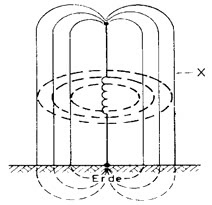
\includegraphics[scale=0.7]{pics/tb306_a.jpg}
	\end{minipage}
\end{center}
\begin{enumerate}[nolistsep,label=\Alph*]
\item Elektrische Feldlinien
\item Magnetische Feldlinien
\item Polarisierte Feldlinien
\item Horizontale Feldlinien
\end{enumerate}


\pagebreak
\subsubsection{Magnetisches Feld}

\paragraph*{TB401 Ein Ringkern hat einen mittleren Durchmesser von 2,6 cm und trägt 6 Windungen Kupferdraht. Wie groß ist die mittlere magnetische Feldstärke im Ringkern, wenn der Strom 2,5 A beträgt?}
\begin{center}
	\begin{minipage}{\linewidth}
		\centering
		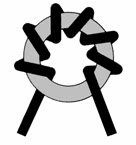
\includegraphics[scale=0.7]{pics/tb401_a.jpg}
	\end{minipage}
\end{center}
\begin{enumerate}[nolistsep,label=\Alph*]
\item 184 $\frac{A}{m}$
\item 1,8 $\frac{A}{m}$
\item 577 $\frac{A}{m}$
\item 5,8 $\frac{A}{m}$
\end{enumerate}



\paragraph*{TB402 Eine Spule ohne Eisenkern erzeugt eine Feldstärke von 200 $\frac{A}{m}$. Wie groß ist die magnetische Flussdichte?}
\begin{enumerate}[nolistsep,label=\Alph*]
\item 0,25 mT
\item 2,5 mT
\item 2,5 T
\item 0,25 T
\end{enumerate}



\paragraph*{TB403 Welcher Effekt verringert die Induktivität einer von hochfrequentem Strom durchflossenen Spule beim Einführen eines Kupfer- oder Aluminiumkerns?}
\begin{enumerate}[nolistsep,label=\Alph*]
\item Das hochfrequente Magnetfeld kann nicht in den Kern eindringen, was den Querschnitt des Feldes verringert.
\item Kupfer und Aluminium sind diamagnetisch und schwächen das Feld ab. 
\item Das leitfähige Metall schließt das Feld kurz. 
\item Kupfer und Aluminium sind unmagnetisch und haben keinen Einfluss auf das Feld.
\end{enumerate}



\paragraph*{TB404 Dauermagnete finden Anwendung in}
\begin{enumerate}[nolistsep,label=\Alph*]
\item Drehspulmesswerken.
\item Dreheisenmesswerken.
\item Transformatorenkernen.
\item Spulenkernen.
\end{enumerate}



\paragraph*{TB405 Wie nennt man das Feld im Innern einer langen Zylinderspule beim Fließen eines Gleichstroms?}
\begin{center}
	\begin{minipage}{\linewidth}
		\centering
		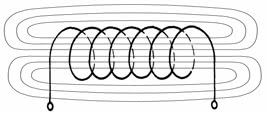
\includegraphics[scale=0.7]{pics/tb405_a.jpg}
	\end{minipage}
\end{center}
\begin{enumerate}[nolistsep,label=\Alph*]
\item Homogenes magnetisches Feld
\item Homogenes elektrisches Feld
\item Konzentrisches magnetisches Feld
\item Zentriertes magnetisches Feld
\end{enumerate}



\paragraph*{TB406 Wenn Strom durch einen gestreckten Leiter fließt, entsteht ein}
\begin{enumerate}[nolistsep,label=\Alph*]
\item Magnetfeld aus konzentrischen Kreisen um den Leiter.
\item elektrisches Feld aus konzentrischen Kreisen um den Leiter.
\item homogenes Magnetfeld um den Leiter.
\item homogenes elektrisches Feld um den Leiter. 
\end{enumerate}



\paragraph*{TB407 Wie werden die mit X gekennzeichneten Feldlinien einer Vertikalantenne bezeichnet?}
\begin{center}
	\begin{minipage}{\linewidth}
		\centering
		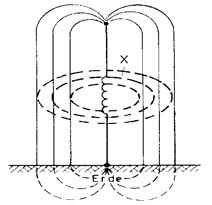
\includegraphics[scale=0.7]{pics/tb407_a.jpg}
	\end{minipage}
\end{center}
\begin{enumerate}[nolistsep,label=\Alph*]
\item Magnetische Feldlinien
\item Elektrische Feldlinien
\item Radiale Feldlinien
\item Vertikale Feldlinien
\end{enumerate}



\paragraph*{TB408 Welches sind die richtigen Einheiten der elektrischen und der magnetischen Feldstärke?}
\begin{enumerate}[nolistsep,label=\Alph*]
\item Elektrische Feldstärke: Volt pro Meter, Magnetische Feldstärke: Ampere pro Meter
\item Elektrische Feldstärke: Ampere pro Meter, Magnetische Feldstärke: Volt pro Meter
\item Elektrische Feldstärke: Volt mal Meter, Magnetische Feldstärke: Ampere mal Meter
\item Elektrische Feldstärke: Ampere mal Meter, Magnetische Feldstärke: Volt mal Meter
\end{enumerate}


\pagebreak
\subsubsection{Elektromagnetisches Feld}

\paragraph*{TB501 Wodurch entsteht ein elektromagnetisches Feld und woraus besteht es?}
\begin{enumerate}[nolistsep,label=\Alph*]
\item Ein elektromagnetisches Feld entsteht, wenn durch einen elektrischen Leiter ein zeitlich schnell veränderlicher Strom fließt. Es besteht aus der elektrischen und aus der magnetischen Feldkomponente (E-Feld und H-Feld).
\item Ein elektromagnetisches Feld entsteht, wenn durch einen elektrischen Leiter ein konstanter Strom fließt. Es besteht aus dem magnetischen Feld (H-Feld), das wiederum ein elektrisches Feld (E-Feld) induziert.
\item Ein elektromagnetisches Feld entsteht, wenn sich elektrische Ladungen in einem Leiter befinden. Es besteht aus dem elektrischen Feld (E-Feld), das wiederum ein magnetisches Feld (H-Feld) induziert.
\item Ein elektromagnetisches Feld entsteht, wenn an einem elektrischen Leiter eine konstante Spannung angelegt wird. Es besteht aus dem elektrischen Feld (E-Feld), das wiederum ein magnetisches Feld (H-Feld) induziert.
\end{enumerate}



\paragraph*{TB502 Wie erfolgt die Ausbreitung einer elektromagnetischen Welle? (Im folgenden Text ist H-Feld die magnetische Feldkomponente und E-Feld die elektrische Feldkomponente.)}
\begin{enumerate}[nolistsep,label=\Alph*]
\item Sie erfolgt durch eine sich ausbreitende Wechselwirkung zwischen E-Feld und H-Feld.
\item Die Ausbreitung erfolgt nur über das E-Feld. Das H-Feld ist nur im Nahfeld vorhanden.
\item Die Ausbreitung erfolgt nur über das H-Feld. Das E-Feld ist nur im Nahfeld vorhanden.
\item E-Feld und H-Feld breiten sich unabhängig voneinander aus und stehen senkrecht zueinander und zur Ausbreitungsrichtung.
\end{enumerate}



\paragraph*{TB503 Die Polarisation einer elektromagnetischen Welle wird durch} 
\begin{enumerate}[nolistsep,label=\Alph*]
\item die Richtung des elektrischen Feldes (Vektor des E-Feldes) angegeben.
\item die Richtung des magnetischen Feldes (Vektor des H-Feldes) angegeben.
\item die Richtung der Ausbreitung (S-Vektor Poyntingscher Vektor) angegeben.
\item die Leistungsflussdichte im Speisepunkt der Antenne bestimmt.
\end{enumerate}



\paragraph*{TB504 Das folgende Bild zeigt die Feldlinien eines elektromagnetischen Feldes. Welche Polarisation hat die skizzierte Wellenfront?}
\begin{center}
	\begin{minipage}{\linewidth}
		\centering
		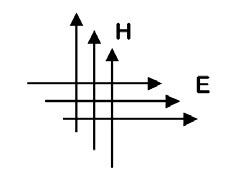
\includegraphics[scale=0.7]{pics/tb504_a.jpg}
	\end{minipage}
\end{center}
\begin{enumerate}[nolistsep,label=\Alph*]
\item Horizontale Polarisation
\item Vertikale Polarisation
\item Rechtsdrehende Polarisation
\item Zirkulare Polarisation
\end{enumerate}



\paragraph*{TB505 Die Polarisation einer elektromagnetischen Welle wird definiert durch}
\begin{enumerate}[nolistsep,label=\Alph*]
\item die Richtung des elektrischen Feldes (E-Vektor).
\item die Richtung des magnetischen Feldes (H-Vektor).
\item die Richtung der Ausbreitung (S-Vektor Poyntingscher Vektor).
\item die räumliche Anordnung der Empfangsantenne.
\end{enumerate}



\paragraph*{TB506 Der Winkel zwischen den E- und HFeldkomponenten eines elektromagnetischen Feldes beträgt im Fernfeld}
\begin{enumerate}[nolistsep,label=\Alph*]
\item $90^{\circ}$.
\item $45^{\circ}$.
\item $180^{\circ}$.
\item $360^{\circ}$.
\end{enumerate}



\paragraph*{TB507 Die Polarisation des Sendesignals in der Hauptstrahlrichtung dieser Richtantenne ist}
\begin{center}
	\begin{minipage}{\linewidth}
		\centering
		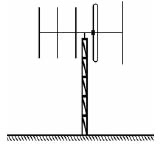
\includegraphics[scale=0.7]{pics/tb507_a.jpg}
	\end{minipage}
\end{center}
\begin{enumerate}[nolistsep,label=\Alph*]
\item vertikal.
\item horizontal.
\item elliptisch.
\item linksdrehend.
\end{enumerate}



\paragraph*{TB508 Welche Aussage trifft auf die elektromagnetische Ausstrahlung im ungestörten Fernfeld zu?}
\begin{enumerate}[nolistsep,label=\Alph*]
\item Die E-Feldkomponente, die H-Feldkomponente und die Ausbreitungsrichtung befinden sich alle in einem rechten Winkel zueinander.
\item Die E-Feldkomponente und die HFeldkomponente befinden sich in einem Winkel von $180^{\circ}$ zueinander. Die Ausbreitungsrichtung verläuft dazu in einem Winkel von $90^{\circ}$.
\item Die E-Feldkomponente und die HFeldkomponente sind phasengleich und befinden sich in einem Winkel von $0^{\circ}$ zueinander. Die Ausbreitungsrichtung verläuft dazu in einem Winkel von $90^{\circ}$.
\item Die Ausbreitungsrichtung befindet sich in einem Winkel von $180^{\circ}$ zur E-Feldkomponente und verläuft parallel zur H-Feldkomponente.
\end{enumerate}



\paragraph*{TB509 Durch welche Größe sind elektrische und magnetische Komponenten eines elektromagnetischen Feldes im Fernfeld miteinander verknüpft?}
\begin{enumerate}[nolistsep,label=\Alph*]
\item Durch den Feldwellenwiderstand des Freiraums
\item Durch die Maxwell-Gleichungen
\item Durch die Ausbreitung in der Ionosphäre
\item Durch die Polarisationsrichtung der Antenne
\end{enumerate}



\paragraph*{TB510 Eine vertikale Dipolantenne wird mit 10 W Senderleistung direkt gespeist. Welche elektrische Feldstärke ergibt sich bei Freiraumausbreitung in 10 m Entfernung?}
\begin{enumerate}[nolistsep,label=\Alph*]
\item 2,2 $\frac{V}{m}$
\item 8,9 $\frac{V}{m}$
\item 0,4 $\frac{V}{m}$
\item 5,5 $\frac{V}{m}$
\end{enumerate}



\paragraph*{TB511 Eine Yagiantenne mit 12,15 dBi Antennengewinn wird mit 250 W Senderleistung direkt gespeist. Welche elektrische Feldstärke ergibt sich bei Freiraumausbreitung in 30 m Entfernung?}
\begin{enumerate}[nolistsep,label=\Alph*]
\item 11,8 $\frac{V}{m}$
\item 9,2 $\frac{V}{m}$
\item 15,1 $\frac{V}{m}$
\item 353 $\frac{V}{m}$
\end{enumerate}



\paragraph*{TB512 Welche elektrische Feldstärke E herrscht in der Mitte der dargestellten, symmetrisch aufgebauten Messzelle, wenn der angeschlossene Sender 1 Watt Ausgangsleistung liefert?}
\begin{center}
	\begin{minipage}{\linewidth}
		\centering
		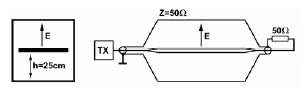
\includegraphics[scale=1.1]{pics/tb512_a.jpg}
	\end{minipage}
\end{center}
\begin{enumerate}[nolistsep,label=\Alph*]
\item 28,3 $\frac{V}{m}$
\item 200 $\frac{V}{m}$
\item 14,1 $\frac{V}{m}$
\item 176,8 $\frac{V}{m}$
\end{enumerate}


\pagebreak
\subsubsection{Sinusförmige Signale}

\paragraph*{TB601 Welche der im folgenden Diagramm eingezeichneten Gleichspannungen ($U_{1}$ ... $U_{6}$) setzen an einem Wirkwiderstand die gleiche Leistung um wie die dargestellte sinusförmige Wechselspannung?}
\begin{center}
	\begin{minipage}{\linewidth}
		\centering
		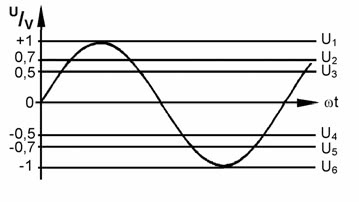
\includegraphics[scale=0.7]{pics/tb601_a.jpg}
	\end{minipage}
\end{center}
\begin{enumerate}[nolistsep,label=\Alph*]
\item $U_{2}$ oder $U_{5}$
\item $U_{1}$ oder $U_{6}$
\item $U_{3}$ oder $U_{4}$
\item nur $U_{2}$
\end{enumerate}



\paragraph*{TB602 Wie groß ist der Spitzen-Spitzen-Wert ($U_{ss}$) der in der Abbildung dargestellten Spannung?}
\begin{center}
	\begin{minipage}{\linewidth}
		\centering
		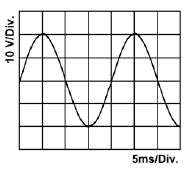
\includegraphics[scale=0.9]{pics/tb602_a.jpg}
	\end{minipage}
\end{center}
\begin{enumerate}[nolistsep,label=\Alph*]
\item 40 Volt
\item 20 Volt
\item 10 Volt
\item 4 Volt
\end{enumerate}



\paragraph*{TB603 Wie groß ist der Spitzen-Spitzen-Wert der in diesem Schirmbild dargestellten Spannung?}
\begin{center}
	\begin{minipage}{\linewidth}
		\centering
		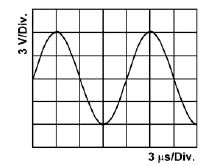
\includegraphics[scale=0.9]{pics/tb603_a.jpg}
	\end{minipage}
\end{center}
\begin{enumerate}[nolistsep,label=\Alph*]
\item 12 Volt
\item 6 Volt
\item 8,5 Volt
\item 2 Volt
\end{enumerate}



\paragraph*{TB604 Welche Frequenz hat die in diesem Oszillogramm dargestellte Spannung?}
\begin{center}
	\begin{minipage}{\linewidth}
		\centering
		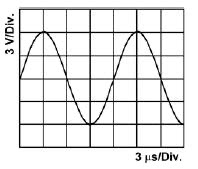
\includegraphics[scale=0.9]{pics/tb604_a.jpg}
	\end{minipage}
\end{center}
\begin{enumerate}[nolistsep,label=\Alph*]
\item 83,3 KHz
\item 833,3 KHz
\item 8,3 MHz
\item 83,3 MHz
\end{enumerate}



\paragraph*{TB605 Welche Frequenz hat das in diesem Schirmbild dargestellte Signal?}
\begin{center}
	\begin{minipage}{\linewidth}
		\centering
		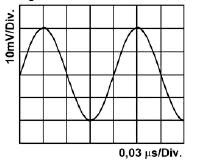
\includegraphics[scale=0.9]{pics/tb605_a.jpg}
	\end{minipage}
\end{center}
\begin{enumerate}[nolistsep,label=\Alph*]
\item 8,33 MHz
\item 16,7 MHz
\item 8,33 KHz
\item 833 KHz
\end{enumerate}



\paragraph*{TB606 Welche Frequenz hat die in diesem Oszillogramm dargestellte Spannung?}
\begin{center}
	\begin{minipage}{\linewidth}
		\centering
		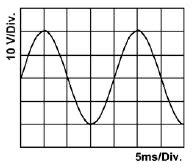
\includegraphics[scale=0.9]{pics/tb606_a.jpg}
	\end{minipage}
\end{center}
\begin{enumerate}[nolistsep,label=\Alph*]
\item 50 Hz
\item 100 Hz
\item 500 Hz
\item 1000 Hz
\end{enumerate}



\paragraph*{TB607 Ein sinusförmiges Signal hat einen Effektivwert von 12 V. Wie groß ist der Spitzen-Spitzen-Wert?}
\begin{enumerate}[nolistsep,label=\Alph*]
\item 33,9 V
\item 24 V
\item 16,97 V
\item 36,4 V
\end{enumerate}



\paragraph*{TB608 Der Spitzenwert der häuslichen 230V-Stromversorgung beträgt}
\begin{enumerate}[nolistsep,label=\Alph*]
\item 325 Volt.
\item 163 Volt.
\item 460 Volt.
\item 650 Volt.
\end{enumerate}



\paragraph*{TB609 Der Spitzen-Spitzen-Wert der häuslichen 230-V-Stromversorgung ist}
\begin{enumerate}[nolistsep,label=\Alph*]
\item 650 Volt.
\item 163 Volt.
\item 325 Volt.
\item 460 Volt.
\end{enumerate}



\paragraph*{TB610 Ein sinusförmiger Wechselstrom mit einer Amplitude (Imax) von 0,5 Ampere fließt durch einen Widerstand von 20 $\Omega$. Wie hoch ist die aufgenommene Leistung?}
\begin{enumerate}[nolistsep,label=\Alph*]
\item 2,5 Watt
\item 5 Watt
\item 10 Watt
\item 0,5 Watt
\end{enumerate}



\paragraph*{TB611 Welche Antwort enthält die richtigen Phasenwinkel einer sinusförmigen Wechselspannung an der mit X3 bezeichneten Stelle?}
\begin{center}
	\begin{minipage}{\linewidth}
		\centering
		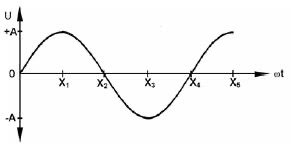
\includegraphics[scale=1.0]{pics/tb611_a.jpg}
	\end{minipage}
\end{center}
\begin{enumerate}[nolistsep,label=\Alph*]
\item $\frac{3\Pi}{2}$; $270^{\circ}$
\item $\frac{\Pi}{3}$; $270^{\circ}$
\item $3\Pi$; $180^{\circ}$
\item $\frac{3\Pi}{4}$; $185^{\circ}$
\end{enumerate}


\paragraph*{TB612 Die Phasendifferenz zwischen den beiden in der Abbildung dargestellten Sinussignalen beträgt}
\begin{center}
	\begin{minipage}{\linewidth}
		\centering
		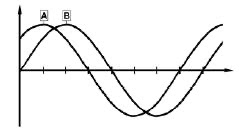
\includegraphics[scale=1.0]{pics/tb612_a.jpg}
	\end{minipage}
\end{center}
\begin{enumerate}[nolistsep,label=\Alph*]
\item $45^{\circ}$.
\item $0^{\circ}$.
\item $90^{\circ}$.
\item $180^{\circ}$.
\end{enumerate}

\pagebreak
\subsubsection{Nichtsinusförmige Signale}
\paragraph*{TB701 Ein symmetrisches Rechtecksignal hat eine Grundfrequenz von 1500 Hz. Welche Frequenzen sind in diesem Signal enthalten?}
\begin{center}
	\begin{minipage}{\linewidth}
		\centering
		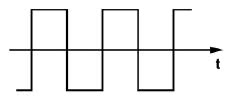
\includegraphics[scale=1.0]{pics/tb701_a.jpg}
	\end{minipage}
\end{center}
\begin{enumerate}[nolistsep,label=\Alph*]
\item 1500 Hz, 4500 Hz, 7500 Hz und höher
\item 1500 Hz, 3000 Hz, 4500 Hz und höher
\item 1500 Hz, 2250 Hz, 3000 Hz und höher
\item 1500 Hz, 3000 Hz, 6000 Hz und höher
\end{enumerate}

\paragraph*{TB702 Die Impulsdauer beträgt hier}
\begin{center}
	\begin{minipage}{\linewidth}
		\centering
		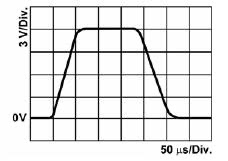
\includegraphics[scale=1.0]{pics/tb702_a.jpg}
	\end{minipage}
\end{center}
\begin{enumerate}[nolistsep,label=\Alph*]
\item 0,2 ms.
\item 260 $\mu$s.
\item 230 $\mu$s.
\item 150 $\mu$s.
\end{enumerate}

\paragraph*{TB703 Was sind Harmonische?}
\begin{enumerate}[nolistsep,label=\Alph*]
\item Harmonische sind die ganzzahligen (1, 2, 3 ...) Vielfachen einer Frequenz.
\item Harmonische sind die ganzzahligen (1, 2, 3 ...) Teile einer Frequenz.
\item Harmonische sind die erzeugten Frequenzen oberhalb der ursprünglichen Frequenz.
\item Harmonische sind identisch mit den Oberwellen, wobei die Grundwelle keine Harmonische ist.
\end{enumerate}

\paragraph*{TB704 Die dritte Oberwelle einer Frequenz ist}
\begin{enumerate}[nolistsep,label=\Alph*]
\item die vierte Harmonische der Frequenz.
\item die dritte Harmonische der Frequenz.
\item die zweite Harmonische der Frequenz.
\item die zweite ungeradzahlige Harmonische der Frequenz.
\end{enumerate}

\paragraph*{TB705 Welche Schwingungen sind in der folgenden Wechselspannung enthalten, wenn die Grundwelle 2 kHz beträgt?}
\begin{center}
	\begin{minipage}{\linewidth}
		\centering
		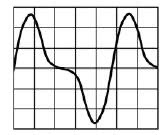
\includegraphics[scale=1.0]{pics/tb705_a.jpg}
	\end{minipage}
\end{center}
\begin{enumerate}[nolistsep,label=\Alph*]
\item 2 KHz und 4 KHz
\item 4 KHz und 6 KHz
\item 4 KHz allein
\item 2 KHz und 6 KHz
\end{enumerate}

\paragraph*{TB706 Welche Schwingungen sind in der folgenden Wechselspannung enthalten, wenn die Grundwelle 2 KHz beträgt?}
\begin{center}
	\begin{minipage}{\linewidth}
		\centering
		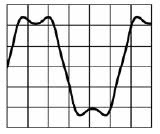
\includegraphics[scale=1.0]{pics/tb706_a.jpg}
	\end{minipage}
\end{center}
\begin{enumerate}[nolistsep,label=\Alph*]
\item 2 KHz und 6 KHz
\item 4 KHz und 6 KHz
\item 2 KHz und 4 KHz
\item 4 KHz allein
\end{enumerate}

\paragraph*{TB707 Die Leistung eines gleichmäßig über einen Frequenzbereich verteilten Rauschens ist}
\begin{enumerate}[nolistsep,label=\Alph*]
\item proportional zur Bandbreite.
\item umgekehrt proportional zur Empfängerempfindlichkeit.
\item proportional zum Signal-Rauschabstand.
\item umgekehrt proportional zum Eingangswiderstand.
\end{enumerate}

\paragraph*{TB708 Wie verhält sich der Pegel des thermischen Rauschens am Empfängerausgang, wenn von einem Quarzfilter mit einer Bandbreite von 2,5 KHz auf ein Quarzfilter mit einer Bandbreite von 0,5 kHz mit gleicher Durchlassdämpfung und Flankensteilheit umgeschaltet wird? Der Rauschpegel}
\begin{enumerate}[nolistsep,label=\Alph*]
\item verringert sich um etwa 7 dB.
\item erhöht sich um etwa 7 dB.
\item verringert sich um etwa 20 dB.
\item erhöht sich um etwa 20 dB.
\end{enumerate}

\pagebreak
\subsubsection{Modulierte Signale}
\paragraph*{TB801 Wie groß ist die HF-Bandbreite, die für die Übertragung eines SSB-Signals erforderlich ist?}
\begin{enumerate}[nolistsep,label=\Alph*]
\item Sie entspricht der Differenz zwischen der höchsten und der niedrigsten Frequenz des NFSignals.
\item Sie entspricht der Hälfte der Bandbreite des NF-Signals.
\item Sie entspricht der doppelten Bandbreite des NF-Signals.
\item Sie ist Null, weil bei SSB-Modulation der HFTräger unterdrückt wird.
\end{enumerate}

\paragraph*{TB802 Ein Träger von 7,05 MHz wird mit der NF-Frequenz von 2 kHz in SSB (LSB) moduliert. Welche Frequenzen treten im modulierten HF-Signal auf?}
\begin{enumerate}[nolistsep,label=\Alph*]
\item 7,048 MHz
\item 7,050 MHz
\item 7,052 MHz
\item 7,048 MHz und 7,052 MHz
\end{enumerate}

\paragraph*{TB803 Ein Träger von 145 MHz wird mit der NF-Frequenz von 2 kHz und einem Hub von 1,8 kHz frequenzmoduliert. Welche Bandbreite hat das modulierte Signal?}
\begin{enumerate}[nolistsep,label=\Alph*]
\item Die Bandbreite beträgt ungefähr 7,6 kHz
\item Die Bandbreite beträgt ungefähr 3,8 kHz
\item Die Bandbreite beträgt ungefähr 5,8 kHz
\item Die Bandbreite beträgt ungefähr 12 kHz
\end{enumerate}

\paragraph*{TB804 Warum wird bei FM senderseitig eine Preemphasis eingesetzt?}
\begin{enumerate}[nolistsep,label=\Alph*]
\item Um das Signal/Rausch-Verhältnis durch Anheben der Amplituden der höheren Modulationsfrequenzen zu verbessern.
\item Um das breitbandige FM-Signal durch Anheben der Amplituden der höheren Modulationsfrequenzen auf Schmalband FM zu reduzieren.
\item Um die Ausgangsleistung durch Verdichtung des Spektrums der Modulationsfrequenzen zu erhöhen.
\item Um das FM Kanalraster von 25 KHz auf 12,5 KHz durch Reduzierung der Bandbreite zu ermöglichen.
\end{enumerate}

\paragraph*{TB805 Kann man auf der Empfängerseite bei Sprachübertragung Frequenz- und Phasenmodulation unterscheiden?}
\begin{enumerate}[nolistsep,label=\Alph*]
\item Nein, im Normalfall ist keine Unterscheidung möglich. 
\item Ja, weil bei Phasenmodulation die Frequenz immer konstant ist.
\item Ja, weil bei Frequenzmodulation ein kräftigeres Signal erzeugt wird.
\item Ja, weil phasenmodulierte Aussendungen in FM-Empfängern bzw. frequenzmodulierte Aussendungen in Phasendiskriminatoren erhebliche Verzerrungen verursachen.
\end{enumerate}

\paragraph*{TB806 Zwei in etwa pegelgleiche Aussendungen können an einer nichtlinear arbeitenden Empfängerstufe}
\begin{enumerate}[nolistsep,label=\Alph*]
\item Intermodulationsprodukte erzeugen.
\item Frequenzmodulation hervorrufen.
\item zwei gleiche Seitenbänder produzieren.
\item einen so genannten Dopplereffekt hervorrufen.
\end{enumerate}

\pagebreak
\subsubsection{Leistung und Energie}
\paragraph*{TB901 Die Ausgangsleistung eines Senders ist}
\begin{enumerate}[nolistsep,label=\Alph*]
\item die unmittelbar nach dem Senderausgang messbare Leistung, bevor sie Zusatzgeräte (z.B. Anpassgeräte) durchläuft.
\item die unmittelbar nach dem Senderausgang gemessene Differenz aus vorlaufender und rücklaufender Leistung.
\item die unmittelbar nach den erforderlichen Zusatzgeräten (z.B. Anpassgeräte) messbare Leistung.
\item die unmittelbar nach dem Senderausgang gemessene Summe aus vorlaufender und rücklaufender Leistung.
\end{enumerate}

\paragraph*{TB902 Die Spitzenleistung eines Senders (PEP) ist}
\begin{enumerate}[nolistsep,label=\Alph*]
\item die durchschnittliche Leistung, die ein Sender unter normalen Betriebsbedingungen während
einer Periode der Hochfrequenzschwingung bei der höchsten Spitze der Modulationshüllkurve der Antennenspeiseleitung zuführt.
\item die unmittelbar nach dem Senderausgang messbare Leistung über die Spitzen der Periode einer durchschnittlichen Hochfrequenzschwingung, bevor Zusatzgeräte (z.B. Anpassgeräte) durchlaufen werden.
\item die durchschnittliche Leistung, die ein Sender unter normalen Betriebsbedingungen an die Antennenspeiseleitung während eines Zeitintervalls abgibt, das im Verhältnis zur Periode der tiefsten Modulationsfrequenz ausreichend lang ist.
\item das Produkt aus der Leistung, die unmittelbar der Antenne zugeführt wird und ihrem Gewinnfaktor in einer Richtung, bezogen auf den Halbwellendipol.
\end{enumerate}

\paragraph*{TB903 Die mittlere Leistung eines Senders ist}
\begin{enumerate}[nolistsep,label=\Alph*]
\item die durchschnittliche Leistung, die ein Sender unter normalen Betriebsbedingungen an die Antennenspeiseleitung während eines Zeitintervalls abgibt, das im Verhältnis zur Periode der tiefsten Modulationsfrequenz ausreichend lang ist.
\item die unmittelbar nach dem Senderausgang messbare Leistung über die Spitzen der Periode einer durchschnittlichen Hochfrequenzschwingung, bevor Zusatzgeräte (z.B. Anpassgeräte) durchlaufen werden.
\item die durchschnittliche Leistung, die ein Sender unter normalen Betriebsbedingungen während einer Periode der Hochfrequenzschwingung bei der höchsten Spitze der Modulationshüllkurve der Antennenspeiseleitung zuführt.
\item das Produkt aus der Leistung, die unmittelbar der Antenne zugeführt wird und ihrem Gewinnfaktor in einer Richtung, bezogen auf den Halbwellendipol.
\end{enumerate}

\paragraph*{TB904 Die äquivalente (effektive) Strahlungsleistung (ERP) ist}
\begin{enumerate}[nolistsep,label=\Alph*]
\item das Produkt aus der Leistung, die unmittelbar der Antenne zugeführt wird und ihrem Gewinnfaktor in einer Richtung, bezogen auf den Halbwellendipol.
\item das Produkt aus der Leistung, die unmittelbar der Antenne zugeführt wird und ihrem Gewinnfaktor in einer Richtung, bezogen auf den isotropen Kugelstrahler.
\item die durchschnittliche Leistung, die ein Sender unter normalen Betriebsbedingungen während einer Periode der Hochfrequenzschwingung bei der höchsten Spitze der Modulationshüllkurve der Antennenspeiseleitung zuführt.
\item die durchschnittliche Leistung, die ein Sender unter normalen Betriebsbedingungen an die Antennenspeiseleitung während eines Zeitintervalls abgibt, das im Verhältnis zur Periode der tiefsten Modulationsfrequenz ausreichend lang ist.
\end{enumerate}

\paragraph*{TB905 Die äquivalente isotrope Strahlungsleistung (EIRP) ist}
\begin{enumerate}[nolistsep,label=\Alph*]
\item das Produkt aus der Leistung, die unmittelbar der Antenne zugeführt wird und ihrem Gewinnfaktor in einer Richtung, bezogen auf den isotropen Kugelstrahler.
\item das Produkt aus der Leistung, die unmittelbar der Antenne zugeführt wird und ihrem Gewinnfaktor in einer Richtung, bezogen auf den Halbwellendipol.
\item die durchschnittliche Leistung, die ein Sender unter normalen Betriebsbedingungen während einer Periode der Hochfrequenzschwingung bei der höchsten Spitze der Modulationshüllkurve der Antennenspeiseleitung zuführt.
\item die durchschnittliche Leistung, die ein Sender unter normalen Betriebsbedingungen an die Antennenspeiseleitung während eines Zeitintervalls abgibt, das im Verhältnis zur Periode der tiefsten Modulationsfrequenz ausreichend lang ist.
\end{enumerate}

\paragraph*{TB906 Die belegte Bandbreite einer Aussendung ist die Frequenzbandbreite,}
\begin{enumerate}[nolistsep,label=\Alph*]
\item bei der die unterhalb ihrer unteren und oberhalb ihrer oberen Frequenzgrenzen ausgesendeten mittleren Leistungen jeweils 0,5 \% der gesamten mittleren Leistung einer gegebenen Aussendung betragen.
\item bei der die oberhalb ihrer unteren und unterhalb ihrer oberen Frequenzgrenzen ausgesendeten mittleren Leistungen jeweils 50 \% der gesamten mittleren Leistung einer gegebenen Aussendung betragen.
\item bei der die oberhalb ihrer unteren und unterhalb ihrer oberen Frequenzgrenzen ausgesendeten mittleren Leistungen jeweils 10 \% der gesamten mittleren Leistung einer gegebenen Aussendung betragen.
\item bei der die unterhalb ihrer unteren und oberhalb ihrer oberen Frequenzgrenzen ausgesendeten mittleren Leistungen jeweils 5 \% der gesamten mittleren Leistung einer gegebenen Aussendung betragen.
\end{enumerate}

\paragraph*{TB907 Was versteht man unter dem Begriff EIRP ?}
\begin{enumerate}[nolistsep,label=\Alph*]
\item Es ist die Leistung, die man einem isotropen Strahler zuführen müsste, damit dieser die gleiche Feldstärke erzeugt wie eine im Vergleich herangezogene reale Antenne, in die eine Antenneneingangsleistung P eingespeist wird.
\item Es ist die Eingangsleistung des verwendeten Senders wie sie in der EMVU-Selbsterklärung anzugeben ist. 
\item Es handelt sich um die Leistung, die man im Maximum der Strahlungskeule einer Dipolantenne vorfindet.
\item Es ist die durchschnittliche Leistung der Amateurfunkstelle wie sie in der EMVU-Selbsterklärung anzugeben ist.

\paragraph*{TB908 Die Spitzenleistung eines Senders ist die}
\begin{enumerate}[nolistsep,label=\Alph*]
\item HF-Leistung bei der höchsten Spitze der Hüllkurve. 
\item Durchschnittsleistung einer SSB-Übertragung.
\item Spitzen-Spitzen-Leistung bei den höchsten Spitzen der Modulationshüllkurve.
\item Mindestleistung bei der Modulationsspitze.
\end{enumerate}

\paragraph*{TB909 Wie wird die ERP (Effective Radiated Power oder auch Equivalent Radiated Power) berechnet und worauf ist sie bezogen?}
\begin{enumerate}[nolistsep,label=\Alph*]
\item ERP = ($P_{Sender}$ - $P_{Verluste}$) * $G_{Antenne}$ bezogen auf den Halbwellendipol
\item ERP = ($P_{Sender}$ * GAntenne) * $P_{Verluste}$ bezogen auf den isotropen Kugelstrahler
\item ERP = ($P_{Sender}$ + $P_{Verluste}$) * $G_{Antenne}$ bezogen auf den Halbwellendipol
\item ERP = $P_{Sender}$ + $P_{Verluste}$ + $G_{Antenne}$ bezogen auf den isotropen Kugelstrahler
\end{enumerate}

\paragraph*{TB910 Wie wird die EIRP ermittelt?}
\begin{enumerate}[nolistsep,label=\Alph*]
\item P_{EIRP} = ($P_{Sender}$ - $P_{Verluste}$) * $G_{Antenne}$ bezogen auf den isotropen Kugelstrahler
\item P_{EIRP} = ($P_{Sender}$ * $G_{Antenne}$) - $P_{Verluste}$ bezogen auf den Halbwellendipol
\item P_{EIRP} = ($P_{Sender}$ + $P_{Verluste}$) * $G_{Antenne}$ bezogen auf den isotropen Kugelstrahler
\item P_{EIRP} = $P_{Sender}$ + $P_{Verluste}$ + $G_{Antenne}$ bezogen auf den Halbwellendipol
\end{enumerate}

\paragraph*{TB911 Um die Störwahrscheinlichkeit zu verringern, sollte die benutzte Sendeleistung}
\begin{enumerate}[nolistsep,label=\Alph*]
\item auf das für eine zufrieden stellende Kommunikation erforderliche Minimum eingestellt werden.
\item nur auf den zulässigen Pegel eingestellt werden. 
\item auf die für eine zufrieden stellende Kommunikation erforderlichen 750 W eingestellt werden.
\item die Hälfte des maximal zulässigen Pegels betragen.
\end{enumerate}

\paragraph*{TB912 Gelten die Formeln für die Leistung an einem Ohmschen Widerstand auch bei Wechselspannung?}
\begin{enumerate}[nolistsep,label=\Alph*]
\item Ja, es sind aber die Effektivwerte einzusetzen. 
\item Nein, denn Spannung und Strom ändern sich laufend.
\item Ja, es darf aber immer nur mit den Spitzenwerten gerechnet werden.
\item Nein, denn Spannung und Strom sind um den Phasenwinkel Phi verschoben.
\end{enumerate}

\paragraph*{TB913 An einem Kondensator mit einer Kapazität von 1 $\mu$F wird eine NF-Spannung von 10 KHz und 12 $V_{eff}$ angelegt. Wie groß ist die aufgenommene Wirkleistung im eingeschwungenen Zustand?}
\begin{enumerate}[nolistsep,label=\Alph*]
\item Fast null Watt
\item 0,9 Watt
\item 0,75 Watt
\item 9 Watt
\end{enumerate}

\paragraph*{TB914 Welche Belastbarkeit muss ein 100-$\Omega$-Widerstand, an dem 10 Volt anliegen, mindestens haben?}
\begin{enumerate}[nolistsep,label=\Alph*]
\item 1 W
\item 0,125 W
\item 10 W
\item 100 mW
\end{enumerate}

\paragraph*{TB915 Eine Glühlampe hat einen Nennwert von 12 V und 48 W. Wie hoch ist die Stromentnahme bei einer 12-V-Versorgung?}
\begin{enumerate}[nolistsep,label=\Alph*]
\item 4 A
\item 250 mA
\item 750 mA
\item 36 A
\end{enumerate}

\paragraph*{TB916 Der Effektivwert der Spannung an einer künstlichen 50-$\Omega$-Antenne wird mit 100 V gemessen. Die Leistung an der Last beträgt}
\begin{enumerate}[nolistsep,label=\Alph*]
\item 200 W.
\item 141 W.
\item 100 W.
\item 283 W.
\end{enumerate}

\paragraph*{TB917 Eine künstliche 50-$\Omega$-Antenne besteht aus elf 560-$\Omega$-Kohleschichtwiderständen mit einem Belastungsnennwert von jeweils 5 W. Wie hoch ist die zulässige Gesamtleistung, die angelegt werden darf?}
\begin{enumerate}[nolistsep,label=\Alph*]
\item 55 W
\item 27,5 W
\item 750 W
\item 5 W
\end{enumerate}

\paragraph*{TB918 Ein mit einer künstlichen 50-$\Omega$-Antenne in Serie geschaltetes Amperemeter zeigt 2 A an. Die Leistung in der Last beträgt}
\begin{enumerate}[nolistsep,label=\Alph*]
\item 200 W.
\item 100 W.
\item 25 W.
\item 250 W.
\end{enumerate}

\paragraph*{TB919 Ein HF-Verstärker ist an eine 12,5-V Gleichstromversorgung angeschlossen. Wenn die HF-Ausgangsleistung des Verstärkers 90 W beträgt, zeigt das an die Stromversorgung angeschlossene Amperemeter 16 A an. Der Wirkungsgrad des Verstärkers beträgt}
\begin{enumerate}[nolistsep,label=\Alph*]
\item 45 \%.
\item 55 \%.
\item 100 \%.
\item 222 \%.
\end{enumerate}

\paragraph*{TB920 Eine HF-Ausgangleistung von 100 W wird in eine angepasste Übertragungsleitung eingespeist. Am antennenseitigen Ende der Leitung beträgt die Leistung 50 W bei einem Stehwellenverhältnis von 1. Wie hoch ist die Leitungsdämpfung?}
\begin{enumerate}[nolistsep,label=\Alph*]
\item 3 $dB$
\item -6 $dB$
\item -3 $dB$
\item 6 $dBm$
\end{enumerate}

\paragraph*{TB921 Ein Spannungsmesser und ein Amperemeter werden für die Ermittlung der Gleichstromeingangsleistung einer Schaltung verwendet. Der Spannungsmesser zeigt 10 V, das Amperemeter 10 A an. Falls beide dabei im Rahmen ihrer Messgenauigkeit jeweils einen um 5 \% zu geringen Wert anzeigen würden, würde man die elektrische Leistung um} 
\begin{enumerate}[nolistsep,label=\Alph*]
\item 9,75 \% zu niedrig bestimmen.
\item 5 \% zu niedrig bestimmen.
\item 10,25 \% zu hoch bestimmen.
\item 5 \% zu hoch bestimmen.
\end{enumerate}

\paragraph*{TB922 An einem Widerstand R wird die elektrische Leistung P in Wärme umgesetzt. Sie kennen die Größen P und R. Nach welcher der Formeln können Sie die Spannung ermitteln, die an dem Widerstand R anliegt?}
\begin{enumerate}[nolistsep,label=\Alph*]
\item $U_{4}$ = $\sqrt{P * R}$
\item $U$ = $R * P$
\item $U$ = $\sqrt{\frac{P}{R}}$
\item $U$ = $\frac{P}{R}$
\end{enumerate}

\paragraph*{TB923 In welcher Antwort sind alle dargestellten Zusammenhänge zwischen Strom, Spannung, Widerstand und Leistung richtig?}
\begin{enumerate}[nolistsep,label=\Alph*]
\item $I$ = $\sqrt{\frac{P}{R}}$ ; $U$ = $\frac{P}{R}$
\item $I$ = $\sqrt{R * R}$; $U$ = $\sqrt{\frac{P}{R}}$
\item $I$ = $\sqrt{\frac{R}{P}}$ ; $U$ = $\frac{P}{R}$
\item $I$ = $\frac{\sqrt{P}}{R}$ ; $U$ = $\sqrt{P}*R$
\end{enumerate}

\paragraph*{TB924 In welcher Antwort sind alle dargestellten Zusammenhänge zwischen Widerstand, Leistung, Spannung und Strom richtig?}
\begin{enumerate}[nolistsep,label=\Alph*]
\item $R$ = $\frac{U^{2}}{P}$; $R$ = $\frac{P}{I^{2}}$
\item $R$ = $U^{2} * P$; $R$ = $\frac{P}{I^{2}}$
\item $R$ = $\frac{P}{U^{2}}$; $R$ = $P * I^{2}$
\item $R$ = $\frac{U^{2}}{P}$; $R$ = $P * I^{2}$
\end{enumerate}

\pagebreak
\subsection{Elektrische und elektronische Bauteile}
\subsubsection{Widerstand}
\paragraph*{TC101 Welche Schaltung könnte dazu verwendet werden, den Wert eines Widerstandes anhand des Ohmschen Gesetzes zu ermitteln?}
\begin{enumerate}[nolistsep,label=\Alph*]
\item 
	\begin{center}
		\begin{minipage}{\linewidth}
			\centering
			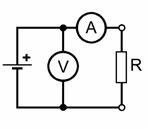
\includegraphics[scale=1.0]{pics/tc101_a.jpg}
		\end{minipage}
	\end{center}
\item
	\begin{center}
		\begin{minipage}{\linewidth}
			\centering
			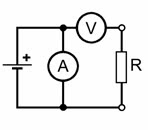
\includegraphics[scale=1.0]{pics/tc101_b.jpg}
		\end{minipage}
	\end{center}
\item 
	\begin{center}
		\begin{minipage}{\linewidth}
			\centering
			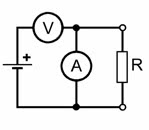
\includegraphics[scale=1.0]{pics/tc101_c.jpg}
		\end{minipage}
	\end{center}
\item
	\begin{center}
		\begin{minipage}{\linewidth}
			\centering
			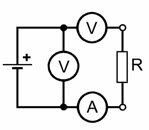
\includegraphics[scale=1.0]{pics/tc101_d.jpg}
		\end{minipage}
	\end{center}
\end{enumerate}

\paragraph*{TC102 Metallschichtwiderstände}
\begin{enumerate}[nolistsep,label=\Alph*]
\item haben geringe Fertigungstoleranzen und Temperaturabhängigkeit und sind besonders als Präzisionswiderstände geeignet.
\item sind induktionsarm und eignen sich besonders für den Einsatz bei sehr hohen Frequenzen. 
\item sind besonders als Hochlastwiderstände bei niedrigen Frequenzen geeignet.
\item haben einen extrem stark negativen Temperaturkoeffizienten und sind besonders als NTC-Widerstände (Heißleiter) geeignet.
\end{enumerate}

\paragraph*{TC103 Metalloxidwiderstände}
\begin{enumerate}[nolistsep,label=\Alph*]
\item sind induktionsarm und eignen sich besonders für den Einsatz bei sehr hohen Frequenzen.
\item haben geringe Toleranzen und Widerstandsänderungen und sind besonders als Präzisionswiderstände in der Messtechnik geeignet.
\item sind besonders als Hochlastwiderstände bei niedrigen Frequenzen geeignet.
\item haben einen extrem stark negativen Temperaturkoeffizienten und sind besonders als NTC-Widerstände (Heißleiter) geeignet.
\end{enumerate}

\paragraph*{TC104 Drahtwiderstände}
\begin{enumerate}[nolistsep,label=\Alph*]
\item sind besonders als Hochlastwiderstände bei niedrigen Frequenzen geeignet.
\item Drahtwiderstände werden hauptsächlich in Form von SMD-Widerständen hergestellt.
\item sind induktionsarm und eignen sich besonders für den Einsatz bei sehr hohen Frequenzen.
\item haben einen extrem stark negativen Temperaturkoeffizienten und sind besonders als NTC-Widerstände (Heißleiter) geeignet.
\end{enumerate}

\paragraph*{TC105 Ein Widerstand von 10 $k\Omega$ hat eine maximale Spannungsfestigkeit von 0,7 kV und eine maximale Belastbarkeit von einem Watt. Welche Gleichspannung darf höchstens an den Widerstand angelegt werden ohne ihn zu überlasten?}
\begin{enumerate}[nolistsep,label=\Alph*]
\item 0,1 kV
\item 10 V
\item 700 V
\item 1 V
\end{enumerate}

\paragraph*{TC106 Ein Widerstand von 50 $k\Omega$ hat eine maximale Spannungsfestigkeit von 0,7 kV und eine maximale Belastbarkeit von 2 Watt. Welche Gleichspannung darf höchstens an den Widerstand angelegt werden ohne ihn zu überlasten?}
\begin{enumerate}[nolistsep,label=\Alph*]
\item 316 V
\item 100 V
\item 25 V
\item 700 V
\end{enumerate}

\paragraph*{TC107 Welche Belastbarkeit muss ein Vorwiderstand haben, an dem bei einem Strom von 48 mA eine Spannung von 208 V abfallen soll?}
\begin{enumerate}[nolistsep,label=\Alph*]
\item 10 W
\item 100 W
\item 4,8 W
\item 0,5 W
\end{enumerate}

\paragraph*{TC108 Ein Widerstand von 120 $\Omega$ hat eine Belastbarkeit von 23 Watt. Welcher Strom darf höchstens durch den Widerstand fließen, damit er nicht überlastet wird?}
\begin{enumerate}[nolistsep,label=\Alph*]
\item 438 mA
\item 192 mA
\item 43,7 mA
\item 2,28 A
\end{enumerate}

\paragraph*{TC109 Ein Widerstand hat eine Toleranz von 10 \%. Bei einem nominalen Widerstandswert von 5,6 $k\Omega$ liegt der tatsächliche Wert zwischen}
\begin{enumerate}[nolistsep,label=\Alph*]
\item 5040 und 6160 $\Omega$.
\item 4760 und 6440 $\Omega$.
\item 4,7 und 6,8 $k\Omega$.
\item 5,2 und 6,3 $k\Omega$.
\end{enumerate}

\paragraph*{TC110 Eine Glühlampe hat einen Nennwert von 12 V und 3 W. Wie viel Strom fließt beim Anschluss an 12 V?}
\begin{enumerate}[nolistsep,label=\Alph*]
\item 250 mA
\item 400 mA
\item 4 A
\item 2,5 A
\end{enumerate}

\paragraph*{TC111 Ein Oszilloskop zeigt einen sinusförmigen Spitze-Spitze-Wert von 25 V an einem 1000-$\Omega$-Widerstand an. Der Effektivstrom durch den Widerstand beträgt}
\begin{enumerate}[nolistsep,label=\Alph*]
\item 8,8 mA.
\item 12,5 mA.
\item 25 mA.
\item 40 A.
\end{enumerate}

\paragraph*{TC112 Ein Lastwiderstand besteht aus zwölf parallelgeschalteten 600-$\Omega$-Drahtwiderständen. Er eignet sich höchstens}
\begin{enumerate}[nolistsep,label=\Alph*]
\item für Tonfrequenzen bis etwa 15 kHz.
\item für Funkfrequenzen bis etwa 144 MHz.
\item für UHF-Senderausgänge mit 50 $\Omega$.
\item als Langdrahtersatz.
\end{enumerate}

\paragraph*{TC113 Eine künstliche Antenne für den VHF-Bereich könnte beispielsweise aus 
\begin{enumerate}[nolistsep,label=\Alph*]
\item ungewendelten Kohleschichtwiderständen zusammengebaut sein.
\item hochbelastbaren Drahtwiderständen zusammengebaut sein.
\item Glühbirnen zusammengebaut sein.
\item temperaturfesten Blindwiderständen bestehen.
\end{enumerate}

\paragraph*{TC114 Welche der folgenden Bauteile könnten für eine genaue künstliche Antenne, die bei 50 MHz eingesetzt werden soll, verwendet werden?}
\begin{enumerate}[nolistsep,label=\Alph*]
\item 10 Kohleschichtwiderstände von 500 $\Omega$
\item ein 50-$\Omega$-Drahtwiderstand
\item 2 parallel geschaltete Drahtwiderstände von 100 $\Omega$
\item ein Spulenanpassfilter im Ölbad
\end{enumerate}

\paragraph*{TC115 Aus welchen Bauteilen sollte eine künstliche Antenne für den VHF-Bereich gebaut werden?}
\begin{enumerate}[nolistsep,label=\Alph*]
\item Aus induktionsarmen Kohleschichtwiderständen
\item Aus Drahtwiderständen mit kapazitätsarmen Anschlusskappen
\item Aus einem abgestimmten Topfkreis mit induktiver Einkopplung
\item Aus versilberten Kupfer-Rundstäben von 10 mm Durchmesser
\end{enumerate}

\pagebreak
\subsubsection{Kondensator}
\paragraph*{TC201 Welche Aussage zur Kapazität eines Plattenkondensators ist richtig?}
\begin{enumerate}[nolistsep,label=\Alph*]
\item Je größer der Plattenabstand ist, desto kleiner ist die Kapazität.
\item Je größer die angelegte Spannung ist, desto kleiner ist die Kapazität.
\item Je größer die Plattenoberfläche ist, desto kleiner ist die Kapazität.
\item Je größer die Dielektrizitätszahl ist, desto kleiner ist die Kapazität.
\end{enumerate}

\paragraph*{TC202 Welchen zeitlichen Verlauf hat die Spannung an einem entladenen Kondensator, wenn dieser über einen Widerstand an eine Gleichspannungsquelle angeschlossen wird?}
\begin{enumerate}[nolistsep,label=\Alph*]
\item
	\begin{center}
		\begin{minipage}{\linewidth}
			\centering
			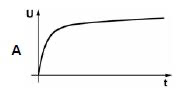
\includegraphics[scale=1.0]{pics/tc202_a.jpg}
		\end{minipage}
	\end{center}
\item
	\begin{center}
		\begin{minipage}{\linewidth}
			\centering
			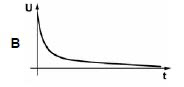
\includegraphics[scale=1.0]{pics/tc202_b.jpg}
		\end{minipage}
	\end{center}
\item
	\begin{center}
		\begin{minipage}{\linewidth}
			\centering
			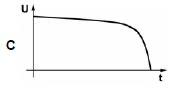
\includegraphics[scale=1.0]{pics/tc202_c.jpg}
		\end{minipage}
	\end{center}
\item
	\begin{center}
		\begin{minipage}{\linewidth}
			\centering
			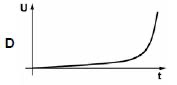
\includegraphics[scale=1.0]{pics/tc202_d.jpg}
		\end{minipage}
	\end{center}
\end{enumerate}

\paragraph*{TC203 Ein verlustloser Kondensator wird an eine Wechselspannungsquelle angeschlossen. Welche Phasenverschiebung zwischen Spannung und Strom stellt sich ein?}
\begin{enumerate}[nolistsep,label=\Alph*]
\item Der Strom eilt der Spannung um $90^{\circ}$ voraus.
\item Die Spannung eilt dem Strom um $90^{\circ}$ voraus.
\item Die Spannung eilt dem Strom um $45^{\circ}$ voraus.
\item Der Strom eilt der Spannung um $45^{\circ}$ voraus.
\end{enumerate}

\paragraph*{TC204 Wie verhält sich der Wechselstromwiderstand eines Kondensators mit zunehmender Frequenz?}
\begin{enumerate}[nolistsep,label=\Alph*]
\item Er nimmt ab.
\item Er bleibt konstant.
\item Er nimmt zu.
\item Er wird unendlich.
\end{enumerate}

\paragraph*{TC205 Wie groß ist der kapazitive Widerstand eines 10-pF-Kondensators bei 100 MHz?}
\begin{enumerate}[nolistsep,label=\Alph*]
\item 159 $\Omega$
\item 1,59 $k\Omega$
\item 318 $\Omega$
\item 31,8 $\Omega$
\end{enumerate}

\paragraph*{TC206 An einem unbekannten Kondensator liegt eine Wechselspannung mit 16 V und 50 Hz. Es wird ein Strom von 32 mA gemessen. Welche Kapazität hat der Kondensator?}
\begin{enumerate}[nolistsep,label=\Alph*]
\item 6,37 $\mu$F
\item 0,637 $\mu$F
\item 0,45 $\mu$F
\item 4,5 $\mu$F
\end{enumerate}

\paragraph*{TC207 Was versteht man unter dem Blindwiderstand eines Kondensators und von welchen physikalischen Größen hängt er ab?}
\begin{enumerate}[nolistsep,label=\Alph*]
\item Der Blindwiderstand ist der mit negativem Vorzeichen versehene Wechselstromwiderstand eines Kondensators. Er ist abhängig von der Kapazität des Kondensators und der anliegenden Frequenz. Im Blindwiderstand entstehen keine Wärmeverluste.
\item Der Blindwiderstand ist der Gleichstromwiderstand eines Kondensators. Er ist abhängig vom Isolationsmaterial des Kondensators und der anliegenden Spannung. Auch im Blindwiderstand entstehen Wärmeverluste.
\item Der Blindwiderstand ist der Wechselstromwiderstand eines Kondensators. Er ist abhängig von der Blindkapazität des Kondensators und der anliegenden Spannung. Im Blindwiderstand entstehen hohe Verluste.
\item Der Blindwiderstand ist der HF- Gleichstromwiderstand eines Kondensators. Er wird mit steigender Kapazität sowie bei erhöhtem Wechselstromanteil und steigender Frequenz größer. Je höher die Frequenz umso eher wandern die Ladungen an die Plattenränder (Skin-Effekt). 
\end{enumerate}

\paragraph*{TC208 Neben dem kapazitiven Blindwiderstand treten im Wechselstrom durchflossenen Kondensator auch Verluste auf, die rechnerisch in einem parallelgeschalteten Verlustwiderstand zusammengefasst werden können.Die Kondensatorverluste werden angegeben durch}
\begin{enumerate}[nolistsep,label=\Alph*]
\item den Verlustfaktor tan $\delta$ (Tangens Delta), der dem Kehrwert des Gütefaktors entspricht.
\item den relativen Verlustwiderstand in $\Omega$ pro Picofarad, mit dem die Kondensatorgüte berechnet werden kann.
\item den relativen Blindwiderstand in $\Omega$ pro Picofarad, mit dem die Kondensatorgüte berechnet werden kann.
\item den Verlustfaktor cos $\phi$ (Cosinus Phi), der dem Kehrwert des Gütefaktors entspricht.
\end{enumerate}

\paragraph*{TC209 Entsteht in einem Wechselstrom durchflossenen Kondensator eine Verlustleistung?}
\begin{enumerate}[nolistsep,label=\Alph*]
\item Ja, infolge von Verlusten im Dielektrikum, die aber meist vernachlässigbar klein sind.
\item Nein, beim Kondensator handelt es sich immer nur um eine reine Blindleistung.
\item Ja, aber nur dann, wenn Luft als Dielektrikum verwendet wird.
\item Ja, genau wie bei Gleichstrom entsprechend den Formeln für Strom, Spannung und Leistung.
\end{enumerate}

\pagebreak
\subsubsection{Spule}
TC301 An eine Spule wird über einen Widerstand eine Gleichspannung angelegt. Welches der nachfolgenden Diagramme zeigt den zeitlichen Verlauf der Spannung über der Spule?
\begin{enumerate}[nolistsep,label=\Alph*]
\item 
	\begin{center}
		\begin{minipage}{\linewidth}
			\centering
			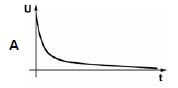
\includegraphics[scale=1.0]{pics/tc301_a.jpg}
		\end{minipage}
	\end{center}
\item
	\begin{center}
		\begin{minipage}{\linewidth}
			\centering
			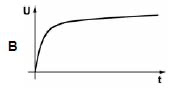
\includegraphics[scale=1.0]{pics/tc301_b.jpg}
		\end{minipage}
	\end{center}
\item
	\begin{center}
		\begin{minipage}{\linewidth}
			\centering
			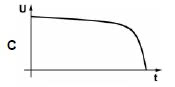
\includegraphics[scale=1.0]{pics/tc301_c.jpg}
		\end{minipage}
	\end{center}
\item
	\begin{center}
		\begin{minipage}{\linewidth}
			\centering
			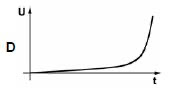
\includegraphics[scale=1.0]{pics/tc301_d.jpg}
		\end{minipage}
	\end{center}
\end{enumerate}

\paragraph*{TC302 In einer reinen Induktivität, die an einer Wechselspannungsquelle angeschlossen ist, eilt der Strom der angelegten Spannung}
\begin{enumerate}[nolistsep,label=\Alph*]
\item um $90^{\circ}$ nach.
\item um $45^{\circ}$ voraus.
\item um $45^{\circ}$ nach.
\item um $90^{\circ}$ voraus.
\end{enumerate}

\paragraph*{TC303 Wie verhält sich der Wechselstromwiderstand einer Spule mit zunehmender Frequenz?}
\begin{enumerate}[nolistsep,label=\Alph*]
\item Er nimmt zu.
\item Er nimmt ab.
\item Er bleibt konstant.
\item Er steigt auf ein Maximum und fällt dann ab.
\end{enumerate}

\paragraph*{TC304 Beim Anlegen einer Gleichspannung U = 1 V an eine Spule messen Sie einen Strom. Wird der Strom beim Anlegen von einer Wechselspannung mit $U_{eff}$ = 1 V größer oder kleiner?}
\begin{enumerate}[nolistsep,label=\Alph*]
\item Beim Betrieb mit Gleichspannung wirkt nur der Gleichstromwiderstand der Spule. Beim Betrieb mit Wechselspannung wird der induktive Widerstand $X_{L}$ wirksam und erhöht den Gesamtwiderstand. Der Strom wird kleiner.
\item Beim Betrieb mit Gleichspannung wirkt nur der Gleichstromwiderstand der Spule. Beim Betrieb mit Wechselspannung wirkt nur der kleinere induktive Widerstand $X_{L}$. Der Strom wird größer. 
\item Beim Betrieb mit Gleich- oder Wechselspannung wirkt nur der $\Omega$sche Widerstand $X_{L}$ der Spule. Der Strom bleibt gleich.
\item Beim Betrieb mit Wechselspannung wirkt nur der Wechselstromwiderstand der Spule. Beim Betrieb mit Gleichspannung wird nur der $\Omega$sche Widerstand $X_{L}$ wirksam. Der Strom wird größer.
\end{enumerate}

\paragraph*{TC305 Wie groß ist der Wechselstromwiderstand einer Spule mit 3 $\mu$H Induktivität bei einer Frequenz von 100 MHz?}
\begin{enumerate}[nolistsep,label=\Alph*]
\item 1885 $\Omega$
\item 942 $\Omega$
\item 1885 $k\Omega$
\item 1,9 $\Omega$
\end{enumerate}

\paragraph*{TC306 Was versteht man unter dem Blindwiderstand einer Spule und von welchen physikalischen Größen hängt er ab?}
\begin{enumerate}[nolistsep,label=\Alph*]
\item Der Blindwiderstand ist der Wechselstromwiderstand einer Spule. Er ist abhängig von der Induktivität der Spule und der anliegenden Frequenz. Im Blindwiderstand entstehen keine Wärmeverluste.
\item Der Blindwiderstand ist der Gleichstromwiderstand einer Spule. Er ist abhängig vom Isolationsmaterial der Spule und der anliegenden Spannung. Auch im Blindwiderstand entstehen Wärmeverluste.
\item Der Blindwiderstand ist der Wechselstromwiderstand einer Spule. Er ist abhängig von der Blindinduktivität der Spule und der anliegenden Spannung. Im Blindwiderstand entstehen hohe Verluste.
\item Der Blindwiderstand ist der HFGleichstromwiderstand einer Spule. Er wird mit steigender Induktivität sowie bei erhöhtem Wechselstromanteil und steigender Frequenz größer. Je tiefer die Frequenz umso eher wandern die Elektronen an den Spulenrand (Skin-Effekt).
\end{enumerate}

\paragraph*{TC307 Neben dem induktiven Blindwiderstand treten in der Wechselstrom durchflossenen Spule auch Verluste auf, die rechnerisch in einem seriellen Verlustwiderstand zusammengefasst werden können. Die Verluste einer Spule werden angegeben durch}
\begin{enumerate}[nolistsep,label=\Alph*]
\item den Verlustfaktor tan $\delta$ (Tangens Delta), der dem Kehrwert des Gütefaktors entspricht.
\item den relativen Verlustwiderstand in $\Omega$ pro Nanohenry, mit dem die Spulengüte berechnet werden kann.
\item den relativen Blindwiderstand in $\Omega$ pro Nanohenry, mit dem die Spulengüte berechnet werden kann.
\item den Verlustfaktor cos $\phi$ (Cosinus Phi), der dem Kehrwert des Gütefaktors entspricht.
\end{enumerate}

\paragraph*{TC308 Hat ein gerades Leiterstück eine Induktivität?}
\begin{enumerate}[nolistsep,label=\Alph*]
\item Ja, jeder Leiter, gleich welche Form er hat, weist eine Induktivität auf.
\item Nein, der Leiter muss wenigstens eine Krümmung (eine viertel, halbe oder ganze Windung) aufweisen.
\item Ja, aber die Größe der Induktivität hängt vom spezifischen Widerstand des Leitermaterials ab.
\item Ja, aber nicht immer, denn abgeschirmte Leiter, beispielsweise Koaxialkabel und Streifenleitungen, weisen nur eine Kapazität auf.
\end{enumerate}

\paragraph*{TC309 Wie kann man die Induktivität einer Spule vergrößern?}
\begin{enumerate}[nolistsep,label=\Alph*]
\item Durch Stauchen der Spule (Verkürzen der Spulenlänge).
\item Durch Auseinanderziehen der Spule (Vergrößerung der Spulenlänge).
\item Durch Einführen eines Kupferkerns in die Spule.
\item Durch Einbau der Spule in einen Abschirmbecher.
\end{enumerate}

\paragraph*{TC310 Mit einem Schalenkern dessen $A_{L}$-Wert mit 250 angegeben ist, soll eine Spule mit einer Induktivität von 2 mH hergestellt werden. Wie groß ist die erforderliche Windungszahl?}
\begin{enumerate}[nolistsep,label=\Alph*]
\item 89
\item 3
\item 2828
\item 53
\end{enumerate}

\paragraph*{TC311 Wie groß ist die Induktivität einer Spule mit 300 Windungen, die auf einen Kern mit einem $A_{L}$-Wert von 1250 gewickelt ist?}
\begin{enumerate}[nolistsep,label=\Alph*]
\item 112,5 mH
\item 112,5 $\mu$H
\item 11,25 mH
\item 1,125 mH
\end{enumerate}

\paragraph*{TC312 Wie groß ist die Induktivität einer Spule mit 14 Windungen, die auf einen Kern mit einem $A_{L}$-Wert von 1,5 gewickelt ist?}
\begin{enumerate}[nolistsep,label=\Alph*]
\item 0,294 $\mu$H
\item 2,94 $\mu$H
\item 29,4 nH
\item 2,94 nH
\end{enumerate}

\paragraph*{TC313 Ein Spulenkern hat einen $A_{L}$-Wert von 30. Wie groß ist die erforderliche Windungszahl zur Herstellung einer Induktivität von 12 $\mu$H?}
\begin{enumerate}[nolistsep,label=\Alph*]
\item 20
\item 400
\item 360
\item 6
\end{enumerate}

\paragraph*{TC314 Welche Folgen hat der Skin-Effekt?}
\begin{enumerate}[nolistsep,label=\Alph*]
\item Der Strom fließt bei hohen Frequenzen nur noch in der Oberfläche des Leiters. Mit sinkendem stromdurchflossenen Querschnitt steigt daher der effektive Widerstand des Leiters.
\item Der Skin-Effekt ist für den mit der Frequenz ansteigenden induktiven Widerstand verantwortlich 
\item Der Strom fließt bei hohen Frequenzen nur noch in der Oberfläche des Leiters. Mit sinkendem stromdurchflossenen Querschnitt steigt daher der induktive Widerstand des Leiters.
\item Der Strom fließt bei hohen Frequenzen nur noch in der Oberfläche des Leiters. Mit sinkendem stromdurchflossenen Querschnitt vergrößert sich daher der kapazitive Widerstand des Leiters.
\end{enumerate}

\paragraph*{TC315 Was verstehen Sie unter dem technischen Ausdruck Skin-Effekt?}
\begin{enumerate}[nolistsep,label=\Alph*]
\item Als Skin-Effekt bezeichnet man die Erscheinung, dass sich mit steigender Frequenz der Elektronenstrom mehr und mehr zur Oberfläche eines Leiters hin verlagert. Dadurch erhöht sich mit steigender Frequenz der $\Omega$sche Leiterwiderstand.
\item Als Skin-Effekt bezeichnet man die Erscheinung, dass sich mit steigender Frequenz der Elektronenstrom mehr und mehr zu den Kanten eines Kondensators hin verlagert. Dadurch erhöht sich mit steigender Frequenz die Kapazität. 
\item Als Skin-Effekt bezeichnet man die Erscheinung, dass sich mit steigender Frequenz die Induktivität und die Kapazität eines Leiters erhöht. Dadurch erhöht sich mit steigendem Leiterwiderstand die Resonanzfrequenz.
\item Als Skin-Effekt bezeichnet man die Erscheinung, dass sich mit steigender Frequenz der Elektronenstrom mehr und mehr zur Leitermitte hin verlagert. Dadurch erhöht sich der $\Omega$sche Leiterwiderstand bei hohem Wechselstromanteil.
\end{enumerate}

\paragraph*{TC316 Das folgende Bild zeigt einen Kern, um den ein Kabel für den Bau einer Netzdrossel gewickelt ist. Der Kern sollte aus}
\begin{center}
	\begin{minipage}{\linewidth}
		\centering
		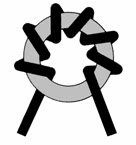
\includegraphics[scale=1.0]{pics/tc316_a.jpg}
	\end{minipage}
\end{center}
\begin{enumerate}[nolistsep,label=\Alph*]
\item Ferrit bestehen.
\item Kunststoff bestehen.
\item Stahl bestehen.
\item paramagnetischem Material bestehen.
\end{enumerate}

\paragraph*{TC317 Für die Unterdrückung parasitärer Schwingungen kann eine verlustbehaftete Drosselspule verwendet werden. Wie wird eine solche Spule gebaut?}
\begin{enumerate}[nolistsep,label=\Alph*]
\item Die Spule wird um einen Widerstand mit niedrigem Widerstandswert gewickelt. 
\item Es wird eine freitragende Spule aus dickem Kupferdraht, der mit einem Silberbelag versehen ist, hergestellt.
\item Es wird ein dicker Kupferdraht um einen Widerstand mit sehr hohem Widerstandswert gewickelt.
\item Es wird ein Kohleschichtwiderstand mit niedrigem Widerstandswert verwendet.
\end{enumerate}

\paragraph*{TC318 Um die Abstrahlungen der Spule eines abgestimmten Schwingkreises zu verringern, sollte die Spule}
\begin{enumerate}[nolistsep,label=\Alph*]
\item in einem Abschirmbecher aus Metall untergebracht werden.
\item in einem nichtmetallischen Harz eingehüllt werden.
\item in einem Abschirmbecher aus Kunststoff untergebracht werden.
\item einen abgestimmten Kunststoffkern aufweisen.
\end{enumerate}

\paragraph*{TC319 Durch Gegeninduktion wird in einer Spule eine Spannung erzeugt, wenn}
\begin{enumerate}[nolistsep,label=\Alph*]
\item ein veränderlicher Strom durch eine magnetisch gekoppelte benachbarte Spule fließt.
\item durch eine magnetisch gekoppelte benachbarte Spule kein Strom fließt.
\item ein konstanter Gleichstrom durch eine magnetisch gekoppelte benachbarte Spule fließt.
\item sich die Spule in einem konstanten Magnetfeld befindet.
\end{enumerate}

\pagebreak
\subsubsection{Übertrager und Transformatoren}
\paragraph*{TC401 Ein Trafo liegt an 230 Volt und gibt 11,5 Volt ab. Seine Primärwicklung hat 600 Windungen. Wie groß ist seine Sekundärwindungszahl?}
\begin{enumerate}[nolistsep,label=\Alph*]
\item 30 Windungen
\item 20 Windungen
\item 52 Windungen
\item 180 Windungen
\end{enumerate}

\paragraph*{TC402 Ein Transformator setzt die Spannung von 230 Volt auf 6 Volt herunter und liefert dabei einen Strom von 1,15 A. Wie groß ist der dadurch in der Primärwicklung zu erwartende Strom bei Vernachlässigung der Verluste?}
\begin{enumerate}[nolistsep,label=\Alph*]
\item 30 mA
\item 22,7 mA
\item 0,83 mA
\item 33,3 mA
\end{enumerate}

\paragraph*{TC403 Eine Transformatorwicklung hat einen Drahtdurchmesser von 0,5 mm. Die zulässige Stromdichte beträgt 2,5 $\frac{A}{mm^{2}}$. Wie groß ist der zulässige Strom?}
\begin{enumerate}[nolistsep,label=\Alph*]
\item 0,49 A
\item 1,96 A
\item 1,25 A
\item 0,23 A
\end{enumerate}

\paragraph*{TC404 In dieser Schaltung ist R = 16 $k\Omega$. Die Impedanz zwischen den Anschlüssen A und B beträgt somit}
\begin{center}
	\begin{minipage}{\linewidth}
		\centering
		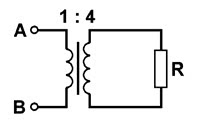
\includegraphics[scale=1.0]{pics/tc404_a.jpg}
	\end{minipage}
\end{center}
\begin{enumerate}[nolistsep,label=\Alph*]
\item 1 $k\Omega$.
\item 64 $k\Omega$.
\item 16 $k\Omega$.
\item 4 $k\Omega$.
\end{enumerate}

\paragraph*{TC405 In dieser Schaltung ist R = 6,4 $k\Omega$. Die Impedanz zwischen den Anschlüssen A und B beträgt somit}
\begin{center}
	\begin{minipage}{\linewidth}
		\centering
		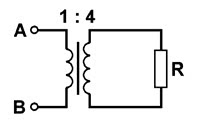
\includegraphics[scale=1.0]{pics/tc405_a.jpg}
	\end{minipage}
\end{center}
\begin{enumerate}[nolistsep,label=\Alph*]
\item 0,4 $k\Omega$.
\item 25,6 $k\Omega$.
\item 6,4 $k\Omega$.
\item 1,6 $k\Omega$.
\end{enumerate}

\paragraph*{TC406 Für die Anpassung einer 300-$\Omega$-Antenne an eine 75-$\Omega$-Übertragungsleitung kann ein Übertrager mit einem Windungszahlenverhältnis von}
\begin{enumerate}[nolistsep,label=\Alph*]
\item 2:1 verwendet werden.
\item 4:1 verwendet werden.
\item 8:1 verwendet werden.
\item 16:1 verwendet werden.
\end{enumerate}

\paragraph*{TC407 Für die Anpassung einer 50-$\Omega$-Übertragungsleitung an eine 600-$\Omega$-Antenne wird ein Übertrager verwendet. Er sollte ein Windungszahlverhältnis von}
\begin{enumerate}[nolistsep,label=\Alph*]
\item 1:3,5 aufweisen.
\item 1:1 aufweisen.
\item 1:5,5 aufweisen.
\item 1:12 aufweisen.
\end{enumerate}

\pagebreak
\subsubsection{Diode}
\paragraph*{TC501 Wie verhalten sich die Elektronen in einem in Durchlassrichtung betriebenen P-N-Übergang?}
\begin{enumerate}[nolistsep,label=\Alph*]
\item Sie wandern von N nach P.
\item Sie wandern von P nach N.
\item Sie bleiben im N-Bereich.
\item Sie zerfallen beim Übergang.
\end{enumerate}

\paragraph*{TC502 Ein in Durchlassrichtung betriebener P-N-Übergang ermöglicht}
\begin{enumerate}[nolistsep,label=\Alph*]
\item den Stromfluss von P nach N.
\item den Stromfluss von N nach P.
\item keinen Stromfluss.
\item den Elektronenfluss von P nach N.
\end{enumerate}

\paragraph*{TC503 Eine in Sperrrichtung betriebene Diode hat}
\begin{enumerate}[nolistsep,label=\Alph*]
\item einen hohen Widerstand.
\item eine hohe Kapazität.
\item eine geringe Impedanz.
\item eine hohe Induktivität.
\end{enumerate}

\paragraph*{TC504 Welche typischen Schwellspannungen haben Germanium- und Siliziumdioden? Sie liegen bei}
\begin{enumerate}[nolistsep,label=\Alph*]
\item Germanium zwischen 0,2 und 0,4 Volt, bei Silizium zwischen 0,5 und 0,8 Volt.
\item Germanium zwischen 0,5 und 0,8 Volt, bei Silizium zwischen 0,2 und 0,4 Volt.
\item Germanium bei etwa 0,7 Volt, bei Silizium bei etwa 0,3 Volt.
\item allen Dioden bei etwa 0,7 Volt.
\end{enumerate}

\paragraph*{TC505 Wie ändert sich die Durchlassspannung einer Diode mit der Temperatur?}
\begin{enumerate}[nolistsep,label=\Alph*]
\item Die Spannung sinkt bei steigender Temperatur.
\item Die Spannung hängt allein vom Durchlassstrom ab.
\item Die Spannung hängt nur vom Trägermaterial ab (Germanium/Silizium).
\item Die Spannung steigt bei wachsender Temperatur.
\end{enumerate}

\paragraph*{TC506 Bei welcher Bedingung wird eine Siliziumdiode leitend?}
\begin{enumerate}[nolistsep,label=\Alph*]
\item An der Anode liegen 5,7 Volt, an der Katode 5,0 Volt an.
\item An der Anode liegen 5,7 Volt, an der Katode 6,4 Volt an.
\item An der Anode liegen 5,0 Volt, an der Katode 5,1 Volt an.
\item An der Anode liegen 5,0 Volt, an der Katode 5,7 Volt an.
\end{enumerate}

\paragraph*{TC507 Die Auswahlantworten enthalten Siliziumdioden mit unterschiedlichen Arbeitspunkten. Bei welcher Antwort befindet sich die Diode in leitendem Zustand?}
\begin{enumerate}[nolistsep,label=\Alph*]
\item 
\item 
\item 
\item 
\end{enumerate}

\paragraph*{TC508 Die Auswahlantworten enthalten Siliziumdioden mit unterschiedlichen Arbeitspunkten. Bei welcher Antwort befindet sich die Diode in leitendem Zustand?}
\begin{enumerate}[nolistsep,label=\Alph*]
\item 
\item 
\item 
\item 
\end{enumerate}

\paragraph*{TC509 Die Auswahlantworten enthalten Siliziumdioden mit unterschiedlichen Arbeitspunkten. Bei welcher Antwort befindet sich die Diode in leitendem Zustand?}
\begin{enumerate}[nolistsep,label=\Alph*]
\item 
\item 
\item 
\item 
\end{enumerate}

\paragraph*{TC510 Die Auswahlantworten enthalten Siliziumdioden mit unterschiedlichen Arbeitspunkten. Bei welcher Antwort befindet sich die Diode in leitendem Zustand?}
\begin{enumerate}[nolistsep,label=\Alph*]
\item 
\item 
\item 
\item 
\end{enumerate}

\paragraph*{TC511 In welcher Zeile sind die Diodentypen der entsprechenden Kennlinie richtig zugeordnet?}
\begin{center}
	\begin{minipage}{\linewidth}
		\centering
		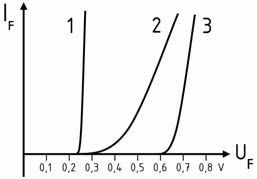
\includegraphics[scale=1.0]{pics/tc511_a.jpg}
	\end{minipage}
\end{center}
\begin{enumerate}[nolistsep,label=\Alph*]
\item 1: Schottkydiode, 2: Germaniumdiode, 3: Siliziumdiode
\item 1: Schottkydiode, 2: Siliziumdiode, 3: Germaniumdiode
\item 1: Germaniumdiode, 2: Schottkydiode, 3: Siliziumdiode
\item 1: Siliziumdiode, 3: Germaniumdiode, 3: Schottkydiode
\end{enumerate}

\paragraph*{TC512 Welche der folgenden Kennlinien ist typisch für eine Germaniumdiode?}
\begin{center}
	\begin{minipage}{\linewidth}
		\centering
		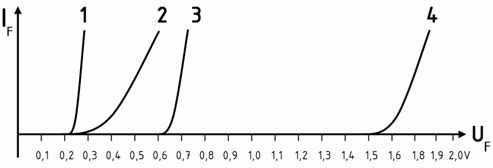
\includegraphics[scale=1.0]{pics/tc512_a.jpg}
	\end{minipage}
\end{center}
\begin{enumerate}[nolistsep,label=\Alph*]
\item Kennlinie 2
\item Kennlinie 1
\item Kennlinie 3
\item Kennlinie 4
\end{enumerate}

\paragraph*{TC513 In welcher Zeile sind die Diodentypen der entsprechenden Kennlinie richtig zugeordnet?}
\begin{center}
	\begin{minipage}{\linewidth}
		\centering
		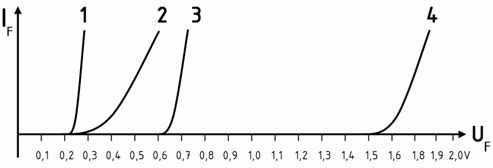
\includegraphics[scale=1.0]{pics/tc513_a.jpg}
	\end{minipage}
\end{center}
\begin{enumerate}[nolistsep,label=\Alph*]
\item Kennlinie 1: Schottkydiode, Kennlinie 2: Germaniumdiode, Kennlinie 3: Siliziumdiode, Kennlinie 4: Leuchtdiode
\item Kennlinie 1: Siliziumdiode, Kennlinie 2: Germaniumdiode, Kennlinie 3: Schottkydiode, Kennlinie 4: Leuchtdiode
\item Kennlinie 1: Schottkydiode, Kennlinie 2: Siliziumdiode, Kennlinie 3: Germaniumdiode, Kennlinie 4: Leuchtdiode
\item Kennlinie 1: Germaniumdiode, Kennlinie 2: Leuchtdiode, Kennlinie 3: Siliziumdiode, Kennlinie 4: Schottkydiode

\paragraph*{TC514 In welcher der folgenden Schaltungen ist die Z-Diode zur Spannungsstabilisierung richtig eingesetzt?}
\begin{enumerate}[nolistsep,label=\Alph*]
\item
	\begin{center}
		\begin{minipage}{\linewidth}
			\centering
			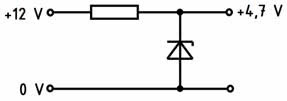
\includegraphics[scale=1.0]{pics/tc514_a.jpg}
		\end{minipage}
	\end{center}
\item
	\begin{center}
		\begin{minipage}{\linewidth}
			\centering
			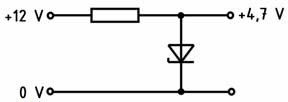
\includegraphics[scale=1.0]{pics/tc514_b.jpg}
		\end{minipage}
	\end{center}
\item
	\begin{center}
		\begin{minipage}{\linewidth}
			\centering
			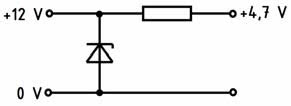
\includegraphics[scale=1.0]{pics/tc514_c.jpg}
		\end{minipage}
	\end{center}
\item
	\begin{center}
		\begin{minipage}{\linewidth}
			\centering
			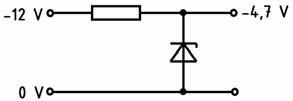
\includegraphics[scale=1.0]{pics/tc514_d.jpg}
		\end{minipage}
	\end{center}
\end{enumerate}

\paragraph*{TC515 In welcher der folgenden Schaltungen ist die Z-Diode zur Spannungsstabilisierung richtig eingesetzt?}
\begin{enumerate}[nolistsep,label=\Alph*]
\item
	\begin{center}
		\begin{minipage}{\linewidth}
			\centering
			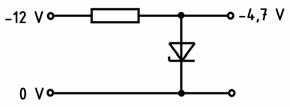
\includegraphics[scale=1.0]{pics/tc515_a.jpg}
		\end{minipage}
	\end{center}
\item
	\begin{center}
		\begin{minipage}{\linewidth}
			\centering
			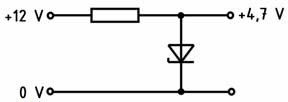
\includegraphics[scale=1.0]{pics/tc515_b.jpg}
		\end{minipage}
	\end{center}
\item
	\begin{center}
		\begin{minipage}{\linewidth}
			\centering
			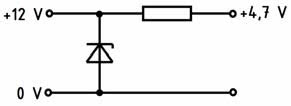
\includegraphics[scale=1.0]{pics/tc515_c.jpg}
		\end{minipage}
	\end{center}
\item
	\begin{center}
		\begin{minipage}{\linewidth}
			\centering
			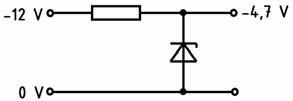
\includegraphics[scale=1.0]{pics/tc515_d.jpg}
		\end{minipage}
	\end{center}
\end{enumerate}

\paragraph*{TC516 Eine unbelastete Z-Diode soll eine 12-VBetriebsspannung auf 5 V stabilisieren. Dabei soll ein Strom von 25 mA durch die Z-Diode fließen. Berechnen Sie den Vorwiderstand. Die Werte des benötigten Vorwiderstandes betragen}
\begin{center}
	\begin{minipage}{\linewidth}
		\centering
		\includegraphics[scale=1.0]{pics/tc516_a.jpg}
	\end{minipage}
\end{center}
\begin{enumerate}[nolistsep,label=\Alph*]
\item 280 $\Omega$ / 175 mW.
\item 280 $\Omega$ / 300 mW.
\item 480 $\Omega$ / 300 mW.
\item 200 $\Omega$ / 175 mW.
\end{enumerate}

\paragraph*{TC517 Folgende Schaltung einer Stabilisierungsschaltung mit Z-Diode ist gegeben. Der Strom durch die Z-Diode soll 25 mA betragen und der Laststrom ist 20 mA. Der Wert des notwendigen Vorwiderstandes beträgt}
\begin{center}
	\begin{minipage}{\linewidth}
		\centering
		\includegraphics[scale=1.0]{pics/tc517_a.jpg}
	\end{minipage}
\end{center}
\begin{enumerate}[nolistsep,label=\Alph*]
\item 202 $\Omega$.
\item 364 $\Omega$.
\item 188 $\Omega$.
\item 235 $\Omega$.
\end{enumerate}

\paragraph*{TC518 Eine Leuchtdiode mit einer Durchlassspannung von 1,4 V und einem Durchlassstrom von 20 mA soll an eine Spannungsquelle von 5,0 V angeschlossen werden. Berechnen Sie den Vorwiderstand. Die Größe des benötigten Vorwiderstandes beträgt}
\begin{enumerate}[nolistsep,label=\Alph*]
\item 180 $\Omega$.
\item 250 $\Omega$.
\item 70 $\Omega$.
\item 320 $\Omega$. 
\end{enumerate}

\paragraph*{TC519 Folgende Schaltung einer Leuchtdiode wird an einer Betriebsspannung von 5,5 V betrieben. Der Strom durch die Leuchtdiode soll 25 mA betragen, wobei die Durchlassspannung 1,75 V beträgt. Der notwendige Vorwiderstand muss folgende Werte haben.}
\begin{center}
	\begin{minipage}{\linewidth}
		\centering
		\includegraphics[scale=1.0]{pics/tc519_a.jpg}
	\end{minipage}
\end{center}
\begin{enumerate}[nolistsep,label=\Alph*]
\item 150 $\Omega$ / 0,1 Watt
\item 220 $\Omega$ / 0,25 Watt
\item 70 $\Omega$ / 0,1 Watt
\item 290 $\Omega$ / 0,25 Watt
\end{enumerate}

\paragraph*{TC520 Wie verändert sich die Frequenz des Schwingkreises in der folgenden Schaltung, wenn das Potentiometer P mehr in Richtung X gedreht wird?}
\begin{center}
	\begin{minipage}{\linewidth}
		\centering
		\includegraphics[scale=1.0]{pics/tc520_a.jpg}
	\end{minipage}
\end{center}
\begin{enumerate}[nolistsep,label=\Alph*]
\item Die Frequenz des Schwingkreises steigt.
\item Die Frequenz des Schwingkreises sinkt.
\item Die Frequenz des Schwingkreises ändert sich nicht.
\item Die Diode sperrt und der Schwingkreis wird unterbrochen.
\end{enumerate}

\paragraph*{TC521 Wie verhält sich die Kapazität einer Kapazitätsdiode (Varicap)?}
\begin{enumerate}[nolistsep,label=\Alph*]
\item Sie nimmt mit abnehmender Sperrspannung zu. 
\item Sie erhöht sich mit zunehmender Durchlassspannung.
\item Sie nimmt mit zunehmender Sperrspannung zu.
\item Sie erhöht sich mit zunehmendem Durchlassstrom.
\end{enumerate}

\paragraph*{TC522 Welches sind die Haupteigenschaften einer Schottkydiode?}
\begin{enumerate}[nolistsep,label=\Alph*]
\item Sehr niedrige Durchlassspannung und sehr hohe Schaltfrequenz.
\item Sehr niedrige Durchlassspannung und sehr niedrige Schaltfrequenz.
\item Sehr hohe Durchlassspannung und sehr hohe Schaltfrequenz.
\item Sehr hohe Durchlassspannung und sehr niedrige Schaltfrequenz.
\end{enumerate}

\paragraph*{TC523 Die Hauptfunktion eines Optokopplers ist}
\begin{enumerate}[nolistsep,label=\Alph*]
\item die Entkopplung zweier Stromkreise.
\item die Erzeugung von Wechselstrom durch Licht.
\item die Abgabe von Licht zur Signalanzeige.
\item die Erzeugung von Gleichstrom durch Licht.
\end{enumerate}

\paragraph*{TC524 Die Hauptfunktion einer Fotodiode ist}
\begin{enumerate}[nolistsep,label=\Alph*]
\item die Umwandlung von Licht in elektrischen Strom.
\item die Abgabe von Licht zur Signalanzeige.
\item die Entkopplung zweier Wechselstromkreise.
\item die Gewinnung von Wechselstrom aus Licht.
\end{enumerate}

\paragraph*{TC525 Das folgende Signal wird als $U_{1}$ an den Eingang der Schaltung mit Siliziumdioden gelegt. Wie sieht das zugehörige Ausgangssignal $U_{2}$ aus?}
\begin{center}
	\begin{minipage}{\linewidth}
		\centering
		\includegraphics[scale=1.0]{pics/tc525_a.jpg}
	\end{minipage}
\end{center}
\begin{center}
	\begin{minipage}{\linewidth}
		\centering
		\includegraphics[scale=1.0]{pics/tc525_b.jpg}
	\end{minipage}
\end{center}
\begin{enumerate}[nolistsep,label=\Alph*]
\item
	\begin{center}
		\begin{minipage}{\linewidth}
			\centering
			\includegraphics[scale=1.0]{pics/tc525_c.jpg}
		\end{minipage}
	\end{center}
\item
	\begin{center}
		\begin{minipage}{\linewidth}
			\centering
			\includegraphics[scale=1.0]{pics/tc525_d.jpg}
		\end{minipage}
	\end{center}
\item
	\begin{center}
		\begin{minipage}{\linewidth}
			\centering
			\includegraphics[scale=1.0]{pics/tc525_e.jpg}
		\end{minipage}
	\end{center}
\item
	\begin{center}
		\begin{minipage}{\linewidth}
			\centering
			\includegraphics[scale=1.0]{pics/tc525_f.jpg}
		\end{minipage}
	\end{center}
\end{enumerate}

\paragraph*{TC526 Das folgende Signal wird als $U_{1}$ an den Eingang der Schaltung mit Germaniumdioden gelegt. Wie sieht das zugehörige Ausgangssignal $U_{2}$ aus?}
	\begin{center}
		\begin{minipage}{\linewidth}
			\centering
			\includegraphics[scale=1.0]{pics/tc526_a.jpg}
		\end{minipage}
	\end{center}
	\begin{center}
		\begin{minipage}{\linewidth}
			\centering
			\includegraphics[scale=1.0]{pics/tc526_b.jpg}
		\end{minipage}
	\end{center}
\begin{enumerate}[nolistsep,label=\Alph*]
\item
	\begin{center}
		\begin{minipage}{\linewidth}
			\centering
			\includegraphics[scale=1.0]{pics/tc526_c.jpg}
		\end{minipage}
	\end{center}
\item
	\begin{center}
		\begin{minipage}{\linewidth}
			\centering
			\includegraphics[scale=1.0]{pics/tc526_d.jpg}
		\end{minipage}
	\end{center}
\item
	\begin{center}
		\begin{minipage}{\linewidth}
			\centering
			\includegraphics[scale=1.0]{pics/tc526_e.jpg}
		\end{minipage}
	\end{center}
\item
	\begin{center}
		\begin{minipage}{\linewidth}
			\centering
			\includegraphics[scale=1.0]{pics/tc526_f.jpg}
		\end{minipage}
	\end{center}
\end{enumerate}

\paragraph*{TC527 In der folgenden Schaltung werden 3 Siliziumdioden zur Entkopplung dreier Stromversorgungen eingesetzt. Der Sonnenkollektor liefert $U_{1}$ = 14,9 V. Der Akkumulator hat $U_{2}$ = 13,9 V. Das Netzteil ist auf $U_{3}$ = 13,5 V eingestellt. In welcher Zeile ist der sich unter diesen Voraussetzungen einstellende Zustand der 3 Dioden richtig beschrieben?}
\begin{center}
	\begin{minipage}{\linewidth}
		\centering
		\includegraphics[scale=1.0]{pics/tc527_a.jpg}
	\end{minipage}
\end{center}
\begin{enumerate}[nolistsep,label=\Alph*]
\item $D_{1}$ leitet. $D_{2}$ leitet. $D_{3}$ leitet nicht.
\item $D_{1}$ leitet. $D_{2}$ leitet. $D_{3}$ leitet.
\item $D_{1}$ leitet. $D_{2}$ leitet nicht. $D_{3}$ leitet nicht.
\item $D_{1}$ leitet nicht. $D_{2}$ leitet. $D_{3}$ leitet.
\end{enumerate}

\paragraph*{TC528 In welcher der folgenden Schaltungen ist die Diode zur Spannungsbegrenzung einer Schaltstufe richtig eingesetzt?}
\begin{enumerate}[nolistsep,label=\Alph*]
\item
	\begin{center}
		\begin{minipage}{\linewidth}
			\centering
			\includegraphics[scale=1.0]{pics/tc528_a.jpg}
		\end{minipage}
	\end{center}
\item
	\begin{center}
		\begin{minipage}{\linewidth}
			\centering
			\includegraphics[scale=1.0]{pics/tc528_b.jpg}
		\end{minipage}
	\end{center}
\item
	\begin{center}
		\begin{minipage}{\linewidth}
			\centering
			\includegraphics[scale=1.0]{pics/tc528_c.jpg}
		\end{minipage}
	\end{center}
\item
	\begin{center}
		\begin{minipage}{\linewidth}
			\centering
			\includegraphics[scale=1.0]{pics/tc528_d.jpg}
		\end{minipage}
	\end{center}
\end{enumerate}

\pagebreak
\subsubsection{Transistor}
\paragraph*{TC601 Welche Bezeichnungen für die Bauelemente sind richtig?}
\begin{center}
	\begin{minipage}{\linewidth}
		\centering
		\includegraphics[scale=1.0]{pics/tc601_a.jpg}
	\end{minipage}
\end{center}
\begin{enumerate}[nolistsep,label=\Alph*]
\item 1: NPN-Transistor 2: PNP-Transistor
\item 1: PNP-Transistor 2: NPN-Transistor
\item 1: N-Kanal-Transistor 2: P-Kanal-Transistor
\item 1: P-Kanal-Transistor 2: N-Kanal-Transistor
\end{enumerate}

\paragraph*{TC602 Welche Bezeichnungen für die Bauelemente sind richtig?}
\begin{center}
	\begin{minipage}{\linewidth}
		\centering
		\includegraphics[scale=1.0]{pics/tc602_a.jpg}
	\end{minipage}
\end{center}
\begin{enumerate}[nolistsep,label=\Alph*]
\item 1: Selbstleitender N-Kanal-Sperrschicht-FET, 2: Selbstleitender P-Kanal-Sperrschicht-FET
\item 1: Selbstsperrender N-Kanal-Sperrschicht-FET, 2: Selbstsperrender P-Kanal-Sperrschicht-FET
\item 1: Selbstleitender P-Kanal-Sperrschicht-FET, 2: Selbstleitender N-Kanal-Sperrschicht-FET
\item 1: Selbstsperrender P-Kanal-Sperrschicht-FET, 2: Selbstsperrender N-Kanal-Sperrschicht-FET
\end{enumerate}

\paragraph*{TC603 Der folgende Transistor ist ein}
\begin{center}
	\begin{minipage}{\linewidth}
		\centering
		\includegraphics[scale=1.0]{pics/tc603_a.jpg}
	\end{minipage}
\end{center}
\begin{enumerate}[nolistsep,label=\Alph*]
\item Selbstsperrender N-Kanal-Isolierschicht FET (MOSFET).
\item Selbstsperrender P-Kanal-Isolierschicht FET (MOSFET).
\item Selbstleitender N-Kanal-Isolierschicht FET (MOSFET).
\item Selbstleitender P-Kanal-Isolierschicht FET (MOSFET).
\end{enumerate}

\paragraph*{TC604 Welcher der folgenden Transistoren ist ein selbstleitender P-Kanal MOSFET?}
\begin{enumerate}[nolistsep,label=\Alph*]
\item
	\begin{center}
		\begin{minipage}{\linewidth}
			\centering
			\includegraphics[scale=1.0]{pics/tc604_a.jpg}
		\end{minipage}
	\end{center}
\item
	\begin{center}
		\begin{minipage}{\linewidth}
			\centering
			\includegraphics[scale=1.0]{pics/tc604_b.jpg}
		\end{minipage}
	\end{center}
\item
	\begin{center}
		\begin{minipage}{\linewidth}
			\centering
			\includegraphics[scale=1.0]{pics/tc604_c.jpg}
		\end{minipage}
	\end{center}
\item
	\begin{center}
		\begin{minipage}{\linewidth}
			\centering
			\includegraphics[scale=1.0]{pics/tc604_d.jpg}
		\end{minipage}
	\end{center}
\end{enumerate}

\paragraph*{TC605 Welcher der folgenden Transistoren ist ein selbstsperrender N-Kanal MOSFET?}
\begin{enumerate}[nolistsep,label=\Alph*]
\item
	\begin{center}
		\begin{minipage}{\linewidth}
			\centering
			\includegraphics[scale=1.0]{pics/tc605_a.jpg}
		\end{minipage}
	\end{center}
\item
	\begin{center}
		\begin{minipage}{\linewidth}
			\centering
			\includegraphics[scale=1.0]{pics/tc605_b.jpg}
		\end{minipage}
	\end{center}
\item
	\begin{center}
		\begin{minipage}{\linewidth}
			\centering
			\includegraphics[scale=1.0]{pics/tc605_c.jpg}
		\end{minipage}
	\end{center}
\item
	\begin{center}
		\begin{minipage}{\linewidth}
			\centering
			\includegraphics[scale=1.0]{pics/tc605_d.jpg}
		\end{minipage}
	\end{center}
\end{enumerate}

\paragraph*{TC606 Wie bezeichnet man die Anschlüsse 2 und 3 des folgenden Transistors?}
\begin{center}
	\begin{minipage}{\linewidth}
		\centering
		\includegraphics[scale=1.0]{pics/tc606_a.jpg}
	\end{minipage}
\end{center}
\begin{enumerate}[nolistsep,label=\Alph*]
\item 2 = Drain, 3 = Source
\item 2 = Source, 3 = Drain
\item 2 = Drain, 3 = Emitter
\item 2 = Gate 2, 3 = Gate 1
\end{enumerate}

\paragraph*{TC607 Welche Kollektorspannungen haben NPN und PNP-Transistoren?}
\begin{enumerate}[nolistsep,label=\Alph*]
\item NPN-Transistoren benötigen positive, PNP-Transistoren negative Kollektorspannungen.
\item NPN- und PNP-Transistoren benötigen negative Kollektorspannungen.
\item PNP-Transistoren benötigen positive, NPN-Transistoren negative Kollektorspannung.
\item PNP- und NPN-Transistoren benötigen positive Kollektorspannungen.
\end{enumerate}

\paragraph*{TC608 Welche Transistortypen sind bipolare Transistoren?}
\begin{enumerate}[nolistsep,label=\Alph*]
\item NPN- und PNP-Transistoren
\item Dual-Gate-MOS-FETs
\item Isolierschicht FETs
\item Sperrschicht FETs
\end{enumerate}

\paragraph*{TC609 Wie erfolgt die Steuerung des Stroms im Feldeffekttransistor (FET)?}
\begin{enumerate}[nolistsep,label=\Alph*]
\item Die Gatespannung steuert den Widerstand des Kanals zwischen Source und Drain.
\item Die Gatespannung steuert den Gatestrom.
\item Der Gatestrom ist allein verantwortlich für den Drainstrom.
\item Der Gatestrom steuert den Widerstand des Kanals zwischen Source und Drain.
\end{enumerate}

\paragraph*{TC610 Wie groß ist der Kollektorstrom eines bipolaren Transistors, wenn die Spannung an seiner Basis die gleiche Höhe hat wie die Spannung an seinem Emitter?}
\begin{enumerate}[nolistsep,label=\Alph*]
\item Es fließt kein Kollektorstrom.
\item Es fließt der maximale Kollektorstrom.
\item Es fließen ca. 5 bis 10 Milliampere.
\item Es fließen je nach Kollektorspannung 0,01 Ampere bis 1 Ampere.
\end{enumerate}

\paragraph*{TC611 Bei welcher Basisspannung ist ein NPN-Transistor ausgeschaltet? Er ist ausgeschaltet bei einer Basisspannung, die}
\begin{enumerate}[nolistsep,label=\Alph*]
\item auf Höhe der Emitterspannung liegt.
\item auf Höhe der Kollektorspannung liegt.
\item zwischen Kollektor und Emitterspannung liegt.
\item mindestens 0,6 V positiver ist, als das Emitterpotenzial.
\end{enumerate}

\paragraph*{TC612 Wie groß ist die Basisspannung eines NPN-Silizium-Transistors, wenn sich dieser in leitendem Zustand befindet?}
\begin{enumerate}[nolistsep,label=\Alph*]
\item Sie ist etwa 0,6 V höher als die Emitterspannung.
\item Sie entspricht der Kollektorspannung.
\item Sie ist viel höher als die Emitterspannung.
\item Sie liegt etwa 0,6V unter der Emitterspannung.
\end{enumerate}

\paragraph*{TC613 Bei einem bipolaren Transistor in leitendem Zustand befindet sich die Emitter-Basis-Diode}
\begin{enumerate}[nolistsep,label=\Alph*]
\item in Durchlassrichtung.
\item im Leerlauf.
\item im Kurzschluss.
\item in Sperrrichtung.
\end{enumerate}

\paragraph*{TC614 In einer Schaltung wurden die Spannungen der Transistoranschlüsse gegenüber Massepotenzial gemessen. Bei welchem der folgenden Transistoren fließt Kollektorstrom?}
\begin{enumerate}[nolistsep,label=\Alph*]
\item
	\begin{center}
		\begin{minipage}{\linewidth}
			\centering
			\includegraphics[scale=1.0]{pics/tc614_a.jpg}
		\end{minipage}
	\end{center}
\item
	\begin{center}
		\begin{minipage}{\linewidth}
			\centering
			\includegraphics[scale=1.0]{pics/tc614_b.jpg}
		\end{minipage}
	\end{center}
\item
	\begin{center}
		\begin{minipage}{\linewidth}
			\centering
			\includegraphics[scale=1.0]{pics/tc614_c.jpg}
		\end{minipage}
	\end{center}
\item
	\begin{center}
		\begin{minipage}{\linewidth}
			\centering
			\includegraphics[scale=1.0]{pics/tc614_d.jpg}
		\end{minipage}
	\end{center}
\end{enumerate}

\paragraph*{TC615 In einer Schaltung wurden die Spannungen der Transistoranschlüsse gegenüber Massepotenzial gemessen. Bei welchem der folgenden Transistoren fließt Kollektorstrom?}
\begin{enumerate}[nolistsep,label=\Alph*]
\item
	\begin{center}
		\begin{minipage}{\linewidth}
			\centering
			\includegraphics[scale=1.0]{pics/tc615_a.jpg}
		\end{minipage}
	\end{center}
\item
	\begin{center}
		\begin{minipage}{\linewidth}
			\centering
			\includegraphics[scale=1.0]{pics/tc615_b.jpg}
		\end{minipage}
	\end{center}
\item
	\begin{center}
		\begin{minipage}{\linewidth}
			\centering
			\includegraphics[scale=1.0]{pics/tc615_c.jpg}
		\end{minipage}
	\end{center}
\item
	\begin{center}
		\begin{minipage}{\linewidth}
			\centering
			\includegraphics[scale=1.0]{pics/tc615_d.jpg}
		\end{minipage}
	\end{center}
\end{enumerate}

\paragraph*{TC616 In einer Schaltung wurden die Spannungen der Transistoranschlüsse gegenüber Massepotenzial gemessen. Bei welchem der folgenden Transistoren fließt Kollektorstrom?}
\begin{enumerate}[nolistsep,label=\Alph*]
\item
	\begin{center}
		\begin{minipage}{\linewidth}
			\centering
			\includegraphics[scale=1.0]{pics/tc616_a.jpg}
		\end{minipage}
	\end{center}
\item
	\begin{center}
		\begin{minipage}{\linewidth}
			\centering
			\includegraphics[scale=1.0]{pics/tc616_b.jpg}
		\end{minipage}
	\end{center}
\item
	\begin{center}
		\begin{minipage}{\linewidth}
			\centering
			\includegraphics[scale=1.0]{pics/tc616_c.jpg}
		\end{minipage}
	\end{center}
\item
	\begin{center}
		\begin{minipage}{\linewidth}
			\centering
			\includegraphics[scale=1.0]{pics/tc616_d.jpg}
		\end{minipage}
	\end{center}
\end{enumerate}

\paragraph*{TC617 In einer Schaltung wurden die Spannungen der Transistoranschlüsse gegenüber Massepotenzial gemessen. Bei welchem der folgenden Transistoren fließt Kollektorstrom?}
\begin{enumerate}[nolistsep,label=\Alph*]
\item
	\begin{center}
		\begin{minipage}{\linewidth}
			\centering
			\includegraphics[scale=1.0]{pics/tc617_a.jpg}
		\end{minipage}
	\end{center}
\item
	\begin{center}
		\begin{minipage}{\linewidth}
			\centering
			\includegraphics[scale=1.0]{pics/tc617_b.jpg}
		\end{minipage}
	\end{center}
\item
	\begin{center}
		\begin{minipage}{\linewidth}
			\centering
			\includegraphics[scale=1.0]{pics/tc617_c.jpg}
		\end{minipage}
	\end{center}
\item
	\begin{center}
		\begin{minipage}{\linewidth}
			\centering
			\includegraphics[scale=1.0]{pics/tc617_d.jpg}
		\end{minipage}
	\end{center}
\end{enumerate}

\paragraph*{TC618 Die Betriebsspannung beträgt 10 V, der Kollektorstrom soll 2 mA betragen, die Gleichstromverstärkung des Transistors beträgt 200. Berechnen Sie den Vorwiderstand $R_{1}$.}
\begin{center}
	\begin{minipage}{\linewidth}
		\centering
		\includegraphics[scale=1.0]{pics/tc618_a.jpg}
	\end{minipage}
\end{center}
\begin{enumerate}[nolistsep,label=\Alph*]
\item 940 $k\Omega$
\item 1 $M\Omega$
\item 85,5 $k\Omega$
\item 47 $k\Omega$
\end{enumerate}

\paragraph*{TC619 Die Betriebsspannung beträgt 10 V, der Kollektorstrom soll 2 mA betragen, die Gleichstromverstärkung des Transistors beträgt 200. Durch den Querwiderstand $R_{2}$ soll der zehnfache Basisstrom fließen. Berechnen Sie den Vorwiderstand $R_{1}$.}
\begin{center}
	\begin{minipage}{\linewidth}
		\centering
		\includegraphics[scale=1.0]{pics/tc619_a.jpg}
	\end{minipage}
\end{center}
\begin{enumerate}[nolistsep,label=\Alph*]
\item 85,5 $k\Omega$
\item 940 $k\Omega$
\item 76,4 $k\Omega$
\item 540 $k\Omega$
\end{enumerate}

\paragraph*{TC620 Die Betriebsspannung beträgt 10 V, der Kollektorstrom soll 2 mA betragen, die Gleichstromverstärkung des Transistors beträgt 200. Durch den Querwiderstand $R_{2}$ soll der zehnfache Basisstrom fließen. Am Emitterwiderstand soll 1 V abfallen. Berechnen Sie den Vorwiderstand $R_{1}$.}
\begin{center}
	\begin{minipage}{\linewidth}
		\centering
		\includegraphics[scale=1.0]{pics/tc620_a.jpg}
	\end{minipage}
\end{center}
\begin{enumerate}[nolistsep,label=\Alph*]
\item 76,4 $k\Omega$
\item 540 $k\Omega$
\item 85,5 $k\Omega$
\item 940 $k\Omega$
\end{enumerate}

\paragraph*{TC621 Die Betriebsspannung beträgt 10 V, der Kollektorstrom soll 2 mA betragen, die Gleichstromverstärkung des Transistors beträgt 200. Die Kollektor-Emitterspannung soll 6 V betragen. Berechnen Sie den Vorwiderstand $R_{1}$.}
\begin{center}
	\begin{minipage}{\linewidth}
		\centering
		\includegraphics[scale=1.0]{pics/tc621_a.jpg}
	\end{minipage}
\end{center}
\begin{enumerate}[nolistsep,label=\Alph*]
\item 540 $k\Omega$
\item 76,4 $k\Omega$
\item 85,5 $k\Omega$
\item 1,98 $k\Omega$
\end{enumerate}

\paragraph*{TC622 Die Betriebsspannung beträgt 10 V, der Kollektorstrom soll 2 mA betragen, die Gleichstromverstärkung des Transistors beträgt 100. Die Kollektor-Emitterspannung soll 6 V betragen. Berechnen Sie den Kollektorwiderstand $R_{C}$.}
\begin{center}
	\begin{minipage}{\linewidth}
		\centering
		\includegraphics[scale=1.0]{pics/tc622_a.jpg}
	\end{minipage}
\end{center}
\begin{enumerate}[nolistsep,label=\Alph*]
\item 1,98 $k\Omega$
\item 20,0 $k\Omega$
\item 85,5 $k\Omega$
\item 2,97 $k\Omega$
\end{enumerate}

\paragraph*{TC623 Was passiert, wenn der Widerstand $R_{2}$ durch eine fehlerhafte Lötstelle an einer Seite keinen Kontakt mehr zur Schaltung hat (Leerlauf)? In welcher Zeile sind beide Aussagen richtig?}
\begin{center}
	\begin{minipage}{\linewidth}
		\centering
		\includegraphics[scale=1.0]{pics/tc623_a.jpg}
	\end{minipage}
\end{center}
\begin{enumerate}[nolistsep,label=\Alph*]
\item Der Kollektorstrom wird nur durch $R_{C}$ begrenzt. Die Kollektorspannung sinkt auf zirka 0,1 Volt.
\item Es fließt Kurzschlussstrom und der Transistor wird zerstört.
\item Es fließt kein Kollektorstrom mehr. Die Kollektorspannung geht auf Betriebsspannung.
\item Der Kollektorstrom steigt stark an. Die Kollektorspannung geht auf Betriebsspannung.
\end{enumerate}

\paragraph*{TC624 Was passiert, wenn der Widerstand $R_{1}$ durch eine fehlerhafte Lötstelle an einer Seite keinen Kontakt mehr zur Schaltung hat (Leerlauf)? In welcher Zeile sind beide Aussagen richtig?}
\begin{center}
	\begin{minipage}{\linewidth}
		\centering
		\includegraphics[scale=1.0]{pics/tc624_a.jpg}
	\end{minipage}
\end{center}
\begin{enumerate}[nolistsep,label=\Alph*]
\item Es fließt kein Kollektorstrom mehr. Die Kollektorspannung geht auf Betriebsspannung.
\item Es fließt Kurzschlussstrom und der Transistor wird zerstört.
\item Der Kollektorstrom wird nur durch RC begrenzt.Die Kollektorspannung sinkt auf zirka 0,1 Volt.
\item Der Kollektorstrom steigt stark an. Die Kollektorspannung geht auf Betriebsspannung.
\end{enumerate}

\paragraph*{TC625 Bei folgender Emitterschaltung wird die Schaltung ohne den Emitterkondensator betrieben. Auf welchen Betrag etwa sinkt die Spannungsverstärkung?}
\begin{center}
	\begin{minipage}{\linewidth}
		\centering
		\includegraphics[scale=1.0]{pics/tc625_a.jpg}
	\end{minipage}
\end{center}
\begin{enumerate}[nolistsep,label=\Alph*]
\item 10
\item $\frac{1}{10}$
\item 1
\item 0
\end{enumerate}

\paragraph*{TC626 Folgendes Signal UE wurde auf den Eingang folgender Schaltung gegeben. In welcher Antwort sind alle dargestellten Signale phasenrichtig zugeordnet?}
\begin{center}
	\begin{minipage}{\linewidth}
		\centering
		\includegraphics[scale=1.0]{pics/tc626_a.jpg}
	\end{minipage}
\end{center}
\begin{center}
	\begin{minipage}{\linewidth}
		\centering
		\includegraphics[scale=1.0]{pics/tc626_b.jpg}
	\end{minipage}
\end{center}
\begin{enumerate}[nolistsep,label=\Alph*]
\item
	\begin{center}
		\begin{minipage}{\linewidth}
			\centering
			\includegraphics[scale=1.0]{pics/tc626_c.jpg}
		\end{minipage}
	\end{center}
\item
	\begin{center}
		\begin{minipage}{\linewidth}
			\centering
			\includegraphics[scale=1.0]{pics/tc626_d.jpg}
		\end{minipage}
	\end{center}
\item
	\begin{center}
		\begin{minipage}{\linewidth}
			\centering
			\includegraphics[scale=1.0]{pics/tc626_e.jpg}
		\end{minipage}
	\end{center}
\item
	\begin{center}
		\begin{minipage}{\linewidth}
			\centering
			\includegraphics[scale=1.0]{pics/tc626_f.jpg}
		\end{minipage}
	\end{center}
\end{enumerate}

\pagebreak
\subsubsection{Einfache digitale und analoge Schaltkreise und sonstige Bauelemente}
\paragraph*{TC701 Eine integrierte Schaltung ist}
\begin{enumerate}[nolistsep,label=\Alph*]
\item eine komplexe Schaltung auf einem Halbleiterkristallblättchen.
\item eine aus einzelnen Bauteilen aufgebaute vergossene Schaltung.
\item eine miniaturisierte, aus SMD-Bauteilen aufgebaute Schaltung.
\item die Zusammenschaltung einzelner Baugruppen zu einem elektronischen Gerät.
\end{enumerate}

\paragraph*{TC702 Welche Funktion hat ein Gatter?}
\begin{enumerate}[nolistsep,label=\Alph*]
\item Ein Gatter verarbeitet binäre Signale nach logischen Grundmustern.
\item Ein Gatter konvertiert digitale Eingangssignale in analoge Ausgangssignale.
\item Ein Gatter ist eine bistabile Kippschaltung, die zwei stabile Zustände (0 und 1) besitzt.
\item Ein Gatter berechnet die Summe oder die Differenz aus zwei binären Ziffern.
\end{enumerate}

\paragraph*{TC703 Wie heißen die Grundbausteine in der Digitaltechnik?}
\begin{enumerate}[nolistsep,label=\Alph*]
\item UND-Glied (AND), ODER-Glied (OR), NICHTUND- Glied (NAND), NICHT-ODER-Glied (NOR).
\item (+)-Gatter (UND), (-)-Gatter (OR), NICHT-(+)-Gatter (NUND), NICHT-(-)-Gatter (NODER).
\item UND-Glied (UND), ODER-Glied (ODER), NICHT-UND-Glied (NUND), NICHT-ODER-Glied (NODER).
\item UND-Gatter (UNG), ODER-Gatter (ORG), NICHT-UND-Gatter (NUNG), NICHT-ODER-Gatter (NORG).
\end{enumerate}

\paragraph*{TC704 Welche der Aussagen trifft für diese Schaltung zu?}
\begin{center}
	\begin{minipage}{\linewidth}
		\centering
		\includegraphics[scale=1.0]{pics/tc704_a.jpg}
	\end{minipage}
\end{center}
\begin{enumerate}[nolistsep,label=\Alph*]
\item X=0 und Y=0
\item X=0 und Y=1
\item X=1 und Y=0
\item X=1 und Y=1
\end{enumerate}

\paragraph*{TC705 Welche logische Grundschaltung stellt die folgende Transistorschaltung dar und wie arbeitet sie?}
	\begin{center}
		\begin{minipage}{\linewidth}
			\centering
			\includegraphics[scale=1.0]{pics/tc705_a.jpg}
		\end{minipage}
	\end{center}
\begin{enumerate}[nolistsep,label=\Alph*]
\item Die Schaltung stellt ein NAND-Gatter [negiertes UND-Gatter] dar. Der Ausgang Z führt dann Nullpotential, wenn die Eingänge A und B mit der Betriebsspannung verbunden sind. In allen anderen Fällen führt der Ausgang Z die Betriebsspannung.
\item Die Schaltung stellt ein NOR-Gatter [negiertes ODER-Gatter] dar. Der Ausgang Z führt dann die Betriebsspannung, wenn keiner der beiden Eingänge A oder B mit der Betriebsspannung verbunden ist. In allen anderen Fällen führt der Ausgang Z Nullpotential.
\item Die Schaltung stellt ein AND-Gatter dar. Der Ausgang Z führt dann Betriebsspannung, wenn die Eingänge A und B mit der Betriebsspannung verbunden sind. In allen anderen Fällen führt der Ausgang Z Nullpotential. 
\item Die Schaltung stellt ein OR-Gatter dar. Der Ausgang Z führt dann Nullpotential, wenn die Eingänge A und B mit der Betriebsspannung verbunden sind. In allen anderen Fällen führt der Ausgang Z die Betriebsspannung.
\end{enumerate}

\paragraph*{TC706 Welche logische Grundschaltung stellt die folgende Transistorschaltung dar und wie arbeitet sie?}
	\begin{center}
		\begin{minipage}{\linewidth}
			\centering
			\includegraphics[scale=1.0]{pics/tc706_a.jpg}
		\end{minipage}
	\end{center}
\begin{enumerate}[nolistsep,label=\Alph*]
\item Die Schaltung stellt ein NOR-Gatter [negiertes ODER-Gatter] dar. Der Ausgang Z führt dann die Betriebsspannung, wenn beide Eingänge A und B Nullpotential führen bzw. offen sind. In allen anderen Fällen führt der Ausgang Z Nullpotential.
\item Die Schaltung stellt ein NAND-Gatter [negiertes UND-Gatter] dar. Der Ausgang Z führt dann Nullpotential, wenn die Eingänge A und B mit der Betriebsspannung verbunden sind. In allen anderen Fällen führt der Ausgang Z die Betriebsspannung.
\item Die Schaltung stellt ein OR-Gatter dar. Der Ausgang Z führt dann Betriebsspannung, wenn die Eingänge A und B mit der Betriebsspannung verbunden sind. In allen anderen Fällen führt der Ausgang Z Nullpotential.
\item Die Schaltung stellt ein AND-Gatter dar. Der Ausgang Z führt dann Nullpotential, wenn die Eingänge A und B mit der Betriebsspannung verbunden sind. In allen anderen Fällen führt der Ausgang Z die Betriebsspannung.
\end{enumerate}

\paragraph*{TC707 Welches der vier im Bild dargestellten Ausgangssignale X1 bis X4 liefert ein ODERGatter, wenn an dessen Eingängen die Signale E1 und E2 anliegen?}
\begin{center}
	\begin{minipage}{\linewidth}
		\centering
		\includegraphics[scale=1.0]{pics/tc707_a.jpg}
	\end{minipage}
\end{center}
\begin{enumerate}[nolistsep,label=\Alph*]
\item X1
\item X2
\item X3
\item X4
\end{enumerate}

\paragraph*{TC708 Welches der vier im Bild dargestellten Ausgangssignale X1 bis X4 liefert ein EXORGatter, wenn an dessen Eingängen die Signale E1 und E2 anliegen?}
\begin{center}
	\begin{minipage}{\linewidth}
		\centering
		\includegraphics[scale=1.0]{pics/tc708_a.jpg}
	\end{minipage}
\end{center}
\begin{enumerate}[nolistsep,label=\Alph*]
\item X3
\item X1
\item X2
\item X4
\end{enumerate}

\paragraph*{TC709 Welches der vier im Bild dargestellten Ausgangssignale X1 bis X4 liefert ein UND-Gatter, wenn an dessen Eingängen die Signale E1 und E2 anliegen?}
\begin{center}
	\begin{minipage}{\linewidth}
		\centering
		\includegraphics[scale=1.0]{pics/tc709_a.jpg}
	\end{minipage}
\end{center}
\begin{enumerate}[nolistsep,label=\Alph*]
\item X2
\item X1
\item X3
\item X4
\end{enumerate}

\paragraph*{TC710 In welchem Versorgungsspannungsbereich können CMOS-ICs betrieben werden?}
\begin{enumerate}[nolistsep,label=\Alph*]
\item +3 V bis +15 V
\item +2,5 V bis +5,5 V
\item $pm$2,5 bis $pm$5,5 V
\item $pm$ 5 V
\end{enumerate}

\paragraph*{TC711 Was ist ein Operationsverstärker?}
\begin{enumerate}[nolistsep,label=\Alph*]
\item Operationsverstärker sind gleichstromgekoppelte Verstärker mit sehr hohem Verstärkungsfaktor und großer Linearität.
\item Operationsverstärker sind wechselstromgekoppelte Verstärker mit niedrigem Eingangswiderstand und großer Linearität.
\item Operationsverstärker sind in Empfängerstufen eingebaute Analogverstärker mit sehr niedrigem Verstärkungsfaktor aber großer Linearität.
\item Operationsverstärker sind digitale Schaltkreise mit niedrigem Verstärkungsfaktor aber großer Linearität.
\end{enumerate}

\paragraph*{TC712 Welche Eigenschaften hat folgende Operationsverstärkerschaltung? In welcher Zeile stimmen alle drei Eigenschaften?}
\begin{center}
	\begin{minipage}{\linewidth}
		\centering
		\includegraphics[scale=1.0]{pics/tc712_a.jpg}
	\end{minipage}
\end{center}
\begin{enumerate}[nolistsep,label=\Alph*]
\item Der Eingangswiderstand ist sehr hoch. Der Ausgangswiderstand ist niedrig. Die Spannungsverstärkung ist gleich eins.
\item Der Eingangswiderstand ist sehr hoch. Der Ausgangswiderstand ist niedrig. Die Spannungsverstärkung ist sehr hoch.
\item Der Eingangswiderstand ist niedrig. Der Ausgangswiderstand ist sehr hoch. Die Spannungsverstärkung ist hoch.
\item Der Eingangswiderstand ist sehr niedrig. Der Ausgangswiderstand ist hoch. Die Spannungsverstärkung ist niedrig.
\end{enumerate}

\paragraph*{TC713 Wie groß ist der Betrag der Spannungsverstärkung UA/UE der folgenden Operationsverstärkerschaltung?}
\begin{center}
	\begin{minipage}{\linewidth}
		\centering
		\includegraphics[scale=1.0]{pics/tc713_a.jpg}
	\end{minipage}
\end{center}
\begin{enumerate}[nolistsep,label=\Alph*]
\item 10
\item 11
\item 19,8
\item 24,2
\end{enumerate}

\paragraph*{TC714 Wie groß ist die Spannungsverstärkung UA/UE der folgenden Operationsverstärkerschaltung?}
\begin{center}
	\begin{minipage}{\linewidth}
		\centering
		\includegraphics[scale=1.0]{pics/tc714_a.jpg}
	\end{minipage}
\end{center}
\begin{enumerate}[nolistsep,label=\Alph*]
\item 11
\item 10
\item 19,8
\item 24,2
\end{enumerate}

\paragraph*{TC715 Der Eingangswiderstand der folgenden Operationsverstärkerschaltung soll 1 $k\Omega$ betragen und es wird eine Spannungsverstärkung von zirka 20 erwünscht. Wie groß muss der Rückkopplungswiderstand $R_{2}$ sein?}
\begin{center}
	\begin{minipage}{\linewidth}
		\centering
		\includegraphics[scale=1.0]{pics/tc715_a.jpg}
	\end{minipage}
\end{center}
\begin{enumerate}[nolistsep,label=\Alph*]
\item zirka 20 $k\Omega$
\item zirka 1 $k\Omega$
\item zirka 400 $k\Omega$
\item zirka 1,9 $k\Omega$
\end{enumerate}

\paragraph*{TC716 Welche der folgenden Operationsverstärkerschaltungen arbeitet als invertierender Spannungsverstärker richtig?}
\begin{enumerate}[nolistsep,label=\Alph*]
\item 
\begin{center}
	\begin{minipage}{\linewidth}
		\centering
		\includegraphics[scale=1.0]{pics/tc716_a.jpg}
	\end{minipage}
\end{center}
\item
\begin{center}
	\begin{minipage}{\linewidth}
		\centering
		\includegraphics[scale=1.0]{pics/tc716_b.jpg}
	\end{minipage}
\end{center}
\item
\begin{center}
	\begin{minipage}{\linewidth}
		\centering
		\includegraphics[scale=1.0]{pics/tc716_c.jpg}
	\end{minipage}
\end{center}
\item
\begin{center}
	\begin{minipage}{\linewidth}
		\centering
		\includegraphics[scale=1.0]{pics/tc716_d.jpg}
	\end{minipage}
\end{center}
\end{enumerate}

\paragraph*{TC717 Welche der folgenden Operationsverstärkerschaltungen arbeitet als nichtinvertierender Spannungsverstärker richtig?}
\begin{enumerate}[nolistsep,label=\Alph*]
\item
\begin{center}
	\begin{minipage}{\linewidth}
		\centering
		\includegraphics[scale=1.0]{pics/tc717_a.jpg}
	\end{minipage}
\end{center}
\item
\begin{center}
	\begin{minipage}{\linewidth}
		\centering
		\includegraphics[scale=1.0]{pics/tc717_b.jpg}
	\end{minipage}
\end{center}
\item
\begin{center}
	\begin{minipage}{\linewidth}
		\centering
		\includegraphics[scale=1.0]{pics/tc717_c.jpg}
	\end{minipage}
\end{center}
\item
\begin{center}
	\begin{minipage}{\linewidth}
		\centering
		\includegraphics[scale=1.0]{pics/tc717_d.jpg}
	\end{minipage}
\end{center}
\end{enumerate}

\paragraph*{TC718 Worauf beruht die Verstärkerwirkung von Elektronenröhren?}
\begin{enumerate}[nolistsep,label=\Alph*]
\item Das von der Gitterspannung hervorgerufene elektrische Feld steuert den Anodenstrom.
\item Die Anodenspannung steuert das magnetische Feld an der Anode und damit den Anodenstrom.
\item Die Heizspannung steuert das elektrische Feld an der Katode und damit den Anodenstrom.
\item Die Katodenvorspannung steuert das magnetische Feld an der Katode und damit den Gitterstrom.
\end{enumerate}

\paragraph*{TC719 In folgender Schaltung mit Elektronenröhre wird die Spannung -Ug am Steuergitter erniedrigt (negativer gemacht). Wie verändert sich der Anodenstrom?}
\begin{center}
	\begin{minipage}{\linewidth}
		\centering
		\includegraphics[scale=1.0]{pics/tc719_a.jpg}
	\end{minipage}
\end{center}
\begin{enumerate}[nolistsep,label=\Alph*]
\item Der Anodenstrom sinkt.
\item Der Anodenstrom steigt.
\item Der Anodenstrom verändert sich nicht.
\item Der Anodenstrom steigt erst und sinkt dann wieder.
\end{enumerate}

\paragraph*{TC720 Berechnen Sie den dezimalen Wert der 8-Bit-Dualzahl 10001110. Die Dezimalzahl lautet}
\begin{enumerate}[nolistsep,label=\Alph*]
\item 142.
\item 78.
\item 156.
\item 248.
\end{enumerate}

\paragraph*{TC721 Wie lautet der dezimale Wert der zweistelligen Hexadezimalzahl 1A? Die Dezimalzahl lautet}
\begin{enumerate}[nolistsep,label=\Alph*]
\item 26.
\item 11.
\item 16.
\item 160.
\end{enumerate}

\paragraph*{TC722 Welche dezimalen Werte haben die Stellen der Dualzahl 111111 von links nach rechts?}
\begin{enumerate}[nolistsep,label=\Alph*]
\item 32, 16, 8, 4, 2, 1
\item 1, 2, 4, 8, 16, 32
\item 65536, 256, 16, 4, 2, 1
\item 100000, 10000, 1000, 100, 10, 1
\end{enumerate}

\pagebreak
\subsection[Elektronische Schaltungen und deren Merkmale}
\subsubsection{Reihen- und Parallelschaltung von Widerständen, Spulen und Kondensatoren}
\paragraph*{TD101 Wie groß ist der Gesamtwiderstand dieser Schaltung, wenn $R_{1}$ = 3,3 $k\Omega$, $R_{2}$ = 4,7 $k\Omega$ und $R_{3}$ = 27 $k\Omega$ betragen?}
\begin{center}
	\begin{minipage}{\linewidth}
		\centering
		\includegraphics[scale=1.0]{pics/td101_a.jpg}
	\end{minipage}
\end{center}
\begin{enumerate}[nolistsep,label=\Alph*]
\item 7,3 $k\Omega$
\item 4,0 $k\Omega$
\item 1,8 $k\Omega$
\item 35 $k\Omega$
\end{enumerate}

\paragraph*{TD102 Eine Reihenschaltung besteht aus drei Kondensatoren von je 0,03 $\mu$F. Wie groß ist die Gesamtkapazität dieser Schaltung?}
\begin{enumerate}[nolistsep,label=\Alph*]
\item 0,01 $\mu$F
\item 0,09 $\mu$F
\item 0,001 $\mu$F
\item 0,009 $\mu$F
\end{enumerate}

\paragraph*{TD103 Wie groß ist die Gesamtkapazität von drei parallel geschalteten Kondensatoren von 20 nF, 0,03 $\mu$F und 15000 pF?}
\begin{enumerate}[nolistsep,label=\Alph*]
\item 0,065 $\mu$F
\item 0,650 $\mu$F
\item 650 nF
\item 650 000 pF
\end{enumerate}

\paragraph*{TD104 Wie groß ist die Gesamtinduktivität von drei in Reihe geschalteten Spulen von 2000 nH, 0,03 mH und 1500 $\mu$H?}
\begin{enumerate}[nolistsep,label=\Alph*]
\item 1532 $\mu$H
\item 1503 $\mu$H
\item 1873 nH
\item 1873 $\mu$H
\end{enumerate}

\paragraph*{TD105 Wie groß ist die Gesamtinduktivität von drei parallel geschalteten Spulen von 2000 nH, 0,03 mH und 1500 $\mu$H?}
\begin{enumerate}[nolistsep,label=\Alph*]
\item 1,873 $\mu$H
\item 187,3 nH
\item 1532 $\mu$H
\item 1,532 $\mu$H
\end{enumerate}

\paragraph*{TD106 Wie groß ist die Gesamtkapazität, wenn drei Kondensatoren $C_{1}$ = 0,06 nF, $C_{2}$ = 40 pF und $C_{3}$ = 20 pF in Reihe geschaltet werden?}
\begin{enumerate}[nolistsep,label=\Alph*]
\item 10,9 pF
\item 0,12 nF
\item 4,1 pF
\item 40 pF
\end{enumerate}

\paragraph*{TD107 Wie groß ist der Gesamtwiderstand der dargestellten Schaltung?}
\begin{center}
	\begin{minipage}{\linewidth}
		\centering
		\includegraphics[scale=1.0]{pics/td107_a.jpg}
	\end{minipage}
\end{center}
\begin{enumerate}[nolistsep,label=\Alph*]
\item 550 $\Omega$
\item 360 $\Omega$
\item 1150 $\Omega$
\item 383 $\Omega$
\end{enumerate}

\paragraph*{TD108 Wie teilt sich die Spannung an zwei in Reihe geschalteten Widerständen auf, wenn $R_{1}$ = 5 mal so groß ist wie $R_{2}$?}
\begin{center}
	\begin{minipage}{\linewidth}
		\centering
		\includegraphics[scale=1.0]{pics/td108_a.jpg}
	\end{minipage}
\end{center}
\begin{enumerate}[nolistsep,label=\Alph*]
\item $U_{1}$ = 5 * $U_{2}$
\item $U_{1}$ = 6 * $U_{2}$
\item $U_{1}$ = $\frac{U_{2}}{5}$
\item $U_{1}$ = $\frac{U_{2}}{6}$
\end{enumerate}

\paragraph*{TD109 Wie teilt sich die Spannung an zwei in Reihe geschalteten Widerständen auf, wenn $R_{1}$ = 1/6 mal so groß ist wie $R_{2}$?}
\begin{center}
	\begin{minipage}{\linewidth}
		\centering
		\includegraphics[scale=1.0]{pics/td109_a.jpg}
	\end{minipage}
\end{center}
\begin{enumerate}[nolistsep,label=\Alph*]
\item $U_{1}$ = $\frac{U_{1}}{6}$
\item $U_{1}$ = 6 * $U_{2}$
\item $U_{1}$ = $\frac{U_{2}}{5}$
\item $U_{1}$ = 5 * $U_{2}$
\end{enumerate}

\paragraph*{TD110 Was ist bei der Berechnung von Wechselstromkreisen, die Kombinationen von R, L und C enthalten, zu beachten?}
\begin{enumerate}[nolistsep,label=\Alph*]
\item Spannungen, Ströme, Widerstände und Leistungen einzelner Komponenten müssen unter Beachtung der Phasenwinkel geometrisch addiert werden.
\item Spannungen, Ströme, Widerstände und Leistungen einzelner Komponenten müssen unter Beachtung der Thomsonschen Schwingungsgleichung addiert werden.
\item An Stelle des $\Omega$schen Gesetzes tritt bei Blindwiderständen im Wechselstromkreis die Thomsonsche Schwingungsgleichung. 
\item Für jede Kombination von R, L und C gelten eigene $\Omega$sche Gesetze.
\end{enumerate}

\paragraph*{TD111 Wie groß ist die Spannung U, wenn durch $R_{3}$ ein Strom von 1 mA fließt und alle Widerstände $R_{1}$ bis $R_{3}$ je 10 $k\Omega$ betragen?}
\begin{center}
	\begin{minipage}{\linewidth}
		\centering
		\includegraphics[scale=1.0]{pics/td111_a.jpg}
	\end{minipage}
\end{center}
\begin{enumerate}[nolistsep,label=\Alph*]
\item 30 V
\item 20 V
\item 15 V
\item 40 V
\end{enumerate}

\paragraph*{TD112 Wie groß ist der Strom durch $R_{3}$, wenn U = 15 V und alle Widerstände $R_{1}$ bis $R_{3}$ je 10 $k\Omega$ betragen?}
\begin{center}
	\begin{minipage}{\linewidth}
		\centering
		\includegraphics[scale=1.0]{pics/td112_a.jpg}
	\end{minipage}
\end{center}
\begin{enumerate}[nolistsep,label=\Alph*]
\item 0,5 mA
\item 1,0 mA
\item 1,6 mA
\item 4,5 mA
\end{enumerate}

\paragraph*{TD113 Welche Leistung tritt in $R_{2}$ auf, wenn U = 15 V und alle Widerstände $R_{1}$ bis $R_{3}$ je 10 $k\Omega$ betragen?}
\begin{center}
	\begin{minipage}{\linewidth}
		\centering
		\includegraphics[scale=1.0]{pics/td113_a.jpg}
	\end{minipage}
\end{center}
\begin{enumerate}[nolistsep,label=\Alph*]
\item 2,5 mW
\item 5,0 mW
\item 1,5 mW
\item 0,15 W
\end{enumerate}

\paragraph*{TD114 Drei gleich große parallel geschaltete Widerstände haben einen Gesamtwiderstand von 1,67 $k\Omega$. Welchen Wert hat jeder Einzelwiderstand?}
\begin{enumerate}[nolistsep,label=\Alph*]
\item 5,0 $k\Omega$
\item 557 $\Omega$
\item 10,0 $k\Omega$
\item 2,5 $k\Omega$
\end{enumerate}

\paragraph*{TD115 Welche Belastbarkeit kann die Zusammenschaltung von drei gleich großen Widerständen mit einer Einzelbelastbarkeit von je 1 W erreichen, wenn alle 3 Widerstände entweder parallel oder in Reihe geschaltet werden?}
\begin{enumerate}[nolistsep,label=\Alph*]
\item 3 W bei Parallel- und bei Reihenschaltung.
\item 3 W bei Parallel- und 1 W bei Reihenschaltung.
\item 1 W bei Parallel- und 3 W bei Reihenschaltung.
\item 1 W bei Parallel- und bei Reihenschaltung.
\end{enumerate}

\paragraph*{TD116 Welche Gesamtkapazität ergibt sich bei einer Parallelschaltung der Kondensatoren 0,1 $\mu$F; 150 nF und 50000 pF?}
\begin{enumerate}[nolistsep,label=\Alph*]
\item 0,3 $\mu$F
\item 0,255 $\mu$F
\item 0,027 $\mu$F
\item 2,73 nF
\end{enumerate}

\paragraph*{TD117 Welche Gesamtkapazität ergibt sich bei einer Reihenschaltung der Kondensatoren 0,1 $\mu$F; 150 nF und 50000 pF?}
\begin{enumerate}[nolistsep,label=\Alph*]
\item 0,027 $\mu$F
\item 2,73 nF
\item 0,3 $\mu$F
\item 0,255 $\mu$F
\end{enumerate}

\paragraph*{TD118 Welche Gesamtkapazität hat diese Schaltung, wenn $C_{1}$ = 0,01 $\mu$F, $C_{2}$ = 5 nF und $C_{3}$ = 5000 pF betragen?}
\begin{center}
	\begin{minipage}{\linewidth}
		\centering
		\includegraphics[scale=1.0]{pics/td118_a.jpg}
	\end{minipage}
\end{center}
\begin{enumerate}[nolistsep,label=\Alph*]
\item 5 nF
\item 12,5 nF
\item 7,5 nF
\item 0,015 nF
\end{enumerate}

\paragraph*{TD119 Welche Gesamtkapazität hat diese Schaltung, wenn $C_{1}$ = 2 $\mu$F, $C_{2}$ = 1 $\mu$F und $C_{3}$ = 1 $\mu$F betragen?
\begin{center}
	\begin{minipage}{\linewidth}
		\centering
		\includegraphics[scale=1.0]{pics/td119_a.jpg}
	\end{minipage}
\end{center}
\begin{enumerate}[nolistsep,label=\Alph*]
\item 1,0 $\mu$F
\item 4400 nF
\item 2,5 $\mu$F
\item 4,0 $\mu$F
\end{enumerate}

\paragraph*{TD120 Wie groß ist die Gesamtkapazität dieser Schaltung, wenn $C_{1}$ = 0,1 nF, $C_{2}$ = 1,5 nF, $C_{3}$ = 220 pF und die Eigenkapazität der Spule 1 pF beträgt?}
\begin{center}
	\begin{minipage}{\linewidth}
		\centering
		\includegraphics[scale=1.0]{pics/td120_a.jpg}
	\end{minipage}
\end{center}
\begin{enumerate}[nolistsep,label=\Alph*]
\item 1821 pF
\item 66 pF
\item 1,6 nF
\item ca. 1 pF
\end{enumerate}

\paragraph*{TD121 Wenn $R_{1}$ und $R_{3}$ je 2 $k\Omega$ hat und $R_{2}$ und $R_{4}$ je 200 $\Omega$ betragen, hat die Schaltung einen Gesamtwiderstand von}
\begin{center}
	\begin{minipage}{\linewidth}
		\centering
		\includegraphics[scale=1.0]{pics/td121_a.jpg}
	\end{minipage}
\end{center}
\begin{enumerate}[nolistsep,label=\Alph*]
\item 1100 $\Omega$.
\item 2200 $\Omega$.
\item 4400 $\Omega$.
\item 2,2 $k\Omega$.
\end{enumerate}

\paragraph*{TD122 In welchem Bereich bewegt sich der Eingangswiderstand der folgenden Schaltung, wenn R alle Werte von 0 bis unendlich durchläuft?}
\begin{center}
	\begin{minipage}{\linewidth}
		\centering
		\includegraphics[scale=1.0]{pics/td122_a.jpg}
	\end{minipage}
\end{center}
\begin{enumerate}[nolistsep,label=\Alph*]
\item 266,7 bis 300 $\Omega$
\item 200 bis 400 $\Omega$
\item 100 bis 200 $\Omega$
\item 300 bis 366,7 $\Omega$
\end{enumerate}

\paragraph*{TD123 Wie groß ist der Gesamtwiderstand dieser Schaltung, wenn $R_{1}$ = 30 $k\Omega$, $R_{2}$ = 15 $k\Omega$, $R_{3}$ = 30 $k\Omega$ und $R_{4}$ = 2,7 $k\Omega$ betragen?}
\begin{center}
	\begin{minipage}{\linewidth}
		\centering
		\includegraphics[scale=1.0]{pics/td123_a.jpg}
	\end{minipage}
\end{center}
\begin{enumerate}[nolistsep,label=\Alph*]
\item 10,2 $k\Omega$
\item 82,7 $k\Omega$
\item 12,7 $k\Omega$
\item 4,5 $k\Omega$
\end{enumerate}

\paragraph*{TD124 Wie groß ist der Gesamtwiderstand dieser Schaltung, wenn $R_{1}$ = 12 $k\Omega$, $R_{2}$ = 12 $k\Omega$, $R_{3}$ = 6 $k\Omega$ und $R_{4}$ = 1,5 $k\Omega$ betragen?}
\begin{center}
	\begin{minipage}{\linewidth}
		\centering
		\includegraphics[scale=1.0]{pics/td124_a.jpg}
	\end{minipage}
\end{center}
\begin{enumerate}[nolistsep,label=\Alph*]
\item 4,5 $k\Omega$
\item 31,5 $k\Omega$
\item 10,2 $k\Omega$
\item 5,5 $k\Omega$
\end{enumerate}

\pagebreak
\subsubsection{Schwingkreise und Filter}
\paragraph*{TD201 Der Impedanzfrequenzgang in der Abbildung zeigt die Kennlinie}
\begin{center}
	\begin{minipage}{\linewidth}
		\centering
		\includegraphics[scale=1.0]{pics/td201_a.jpg}
	\end{minipage}
\end{center}
\begin{enumerate}[nolistsep,label=\Alph*]
\item eines Serienschwingkreises.
\item eines Parallelschwingkreises.
\item einer Induktivität.
\item einer Kapazität.
\end{enumerate}

\paragraph*{TD202 Der im folgenden Bild dargestellte Impedanzfrequenzgang ist typisch für}
\begin{center}
	\begin{minipage}{\linewidth}
		\centering
		\includegraphics[scale=1.0]{pics/td202_a.jpg}
	\end{minipage}
\end{center}
\begin{enumerate}[nolistsep,label=\Alph*]
\item einen Parallelschwingkreis.
\item einen Kondensator.
\item eine Spule.
\item einen Serienschwingkreis.
\end{enumerate}

\paragraph*{TD203 Was ist im Resonanzfall bei der Reihenschaltung einer Induktivität mit einer Kapazität erfüllt?}
\begin{enumerate}[nolistsep,label=\Alph*]
\item Der Betrag des induktiven Widerstands ist dann gleich dem Betrag des kapazitiven Widerstands. 
\item Der Wert des Verlustwiderstands der Spule ist dann gleich dem Wert des Verlustwiderstands des Kondensators.
\item Die Größe des elektrischen Feldes in der Spule ist dann gleich der Größe des elektrischen Feldes im Kondensators.
\item Die Größe des magnetischen Feldes in der Spule ist dann gleich der Größe des magnetischen Feldes im Kondensator.
\end{enumerate}

\paragraph*{TD204 Welcher Schwingkreis passt zu dem neben der jeweiligen Schaltung dargestellten Verlauf des Scheinwiderstandes?}
\begin{enumerate}[nolistsep,label=\Alph*]
\item
\begin{center}
	\begin{minipage}{\linewidth}
		\centering
		\includegraphics[scale=1.0]{pics/td204_a.jpg}
	\end{minipage}
\end{center}
\item
\begin{center}
	\begin{minipage}{\linewidth}
		\centering
		\includegraphics[scale=1.0]{pics/td204_b.jpg}
	\end{minipage}
\end{center}
\item
\begin{center}
	\begin{minipage}{\linewidth}
		\centering
		\includegraphics[scale=1.0]{pics/td204_c.jpg}
	\end{minipage}
\end{center}
\item
\begin{center}
	\begin{minipage}{\linewidth}
		\centering
		\includegraphics[scale=1.0]{pics/td204_d.jpg}
	\end{minipage}
\end{center}
\end{enumerate}

\paragraph*{TD205 Kann die Wicklung eines Übertragers zusammen mit einem Kondensator als Schwingkreis dienen?}
\begin{enumerate}[nolistsep,label=\Alph*]
\item Ja, die Wicklung des Übertragers dient dann als Schwingkreisinduktivität.
\item Nein, ein Übertrager kann nur Spannungen und Ströme umsetzen.
\item Ja, es geht dann die Summe der Induktivitäten beider Wicklungen des Übertragers ein.
\item Ja, aber zu jeder Wicklung muss ein passend gewählter Kondensator in Reihe geschaltet werden.
\end{enumerate}

\paragraph*{TD206 Wie ändert sich die Resonanzfrequenz eines Schwingkreises, wenn 1. die Spule mehr Windungen erhält, 2. die Länge der Spule durch Zusammenschieben der Drahtwicklung verringert wird, 3. ein Kupferkern in das Innere der Spule gebracht wird?}
\begin{enumerate}[nolistsep,label=\Alph*]
\item Die Resonanzfrequenz wird bei 1. und 2. kleiner und bei 3. größer. 
\item Die Resonanzfrequenz wird in allen drei Fällen kleiner.
\item Die Resonanzfrequenz wird bei 1. kleiner und bei 2. und 3. größer. 
\item Die Resonanzfrequenz wird bei 1. und 2. größer und bei 3. kleiner.
\end{enumerate}

\paragraph*{TD207 Wie groß ist die Resonanzfrequenz dieser Schaltung, wenn $C_{1}$ = 0,1 nF, $C_{2}$ = 1,5 nF, $C_{3}$ = 220 pF und L = 1 mH beträgt?}
\begin{center}
	\begin{minipage}{\linewidth}
		\centering
		\includegraphics[scale=1.0]{pics/td207_a.jpg}
	\end{minipage}
\end{center}
\begin{enumerate}[nolistsep,label=\Alph*]
\item 117,973 KHz
\item 11,797 KHz
\item 1,18 KHz
\item 1,17973 MHz
\end{enumerate}

\paragraph*{TD208 Welche Resonanzfrequenz $f_{res}$ hat die Reihenschaltung einer Spule von 100 $\mu$H mit einem Kondensator von 0,01 $\mu$F und einem Widerstand von 100 $\Omega$?}
\begin{enumerate}[nolistsep,label=\Alph*]
\item 159,155 KHz
\item 15,9155 KHz
\item 1,59155 KHz
\item 1591,55 KHz
\end{enumerate}

\paragraph*{TD209 Welche Resonanzfrequenz $f_{res}$ hat die Parallelschaltung einer Spule von 2 $\mu$H mit einem Kondensator von 60 pF und einem Widerstand von 10 $k\Omega$?}
\begin{enumerate}[nolistsep,label=\Alph*]
\item 14,5288 MHz
\item 145,288 MHz
\item 1,45288 MHz
\item 145,288 KHz
\end{enumerate}

\paragraph*{TD210 Wie groß ist die Resonanzfrequenz dieser Schaltung, wenn C = 6,8 pF, R = 10 $\Omega$ und L = 1 $\mu$H beträgt?}
\begin{center}
	\begin{minipage}{\linewidth}
		\centering
		\includegraphics[scale=1.0]{pics/td210_a.jpg}
	\end{minipage}
\end{center}
\begin{enumerate}[nolistsep,label=\Alph*]
\item 61,033 MHz
\item 6,1033 MHz
\item 610,33 MHz
\item 610,33 KHz
\end{enumerate}

\paragraph*{TD211 Wie groß ist die Resonanzfrequenz dieser Schaltung, wenn C = 1 nF, R = 0,1 $k\Omega$ und L = 10 $\mu$H beträgt?}
\begin{center}
	\begin{minipage}{\linewidth}
		\centering
		\includegraphics[scale=1.0]{pics/td211_a.jpg}
	\end{minipage}
\end{center}
\begin{enumerate}[nolistsep,label=\Alph*]
\item 1,592 MHz
\item 159,155 KHz
\item 15,915 MHz
\item 15,915 KHz
\end{enumerate}

\paragraph*{TD212 Bei Resonanz ist die Impedanz dieser Schaltung}
\begin{center}
	\begin{minipage}{\linewidth}
		\centering
		\includegraphics[scale=1.0]{pics/td212_a.jpg}
	\end{minipage}
\end{center}
\begin{enumerate}[nolistsep,label=\Alph*]
\item gleich dem reellen Widerstand R.
\item unendlich hoch.
\item gleich dem kapazitiven Widerstand XC.
\item gleich dem induktiven Widerstand XL.
\end{enumerate}

\parapraph*{TD213 Welche Grenzfrequenz ergibt sich bei einem Tiefpass mit einem Widerstand von 10 $k\Omega$ und einem Kondensator von 50 nF?}
\begin{center}
	\begin{minipage}{\linewidth}
		\centering
		\includegraphics[scale=1.0]{pics/td213_a.jpg}
	\end{minipage}
\end{center}
\begin{enumerate}[nolistsep,label=\Alph*]
\item 318 Hz
\item 0,32 Hz
\item 318 KHz
\item 421 Hz
\end{enumerate}

\paragraph*{TD214 Welchen Gütefaktor Q hat die Reihenschaltung einer Spule von 100 $\mu$H mit einem Kondensator von 0,01 $\mu$F und einem Widerstand von 10 $\Omega$?}
\begin{enumerate}[nolistsep,label=\Alph*]
\item 10
\item 1
\item 0,1
\item 100
\end{enumerate}

\paragraph*{TD215 Welchen Gütefaktor Q hat die Parallelschaltung einer Spule von 2 $\mu$H mit einem Kondensator von 60 pF und einem Widerstand von 1 $k\Omega$?}
\begin{enumerate}[nolistsep,label=\Alph*]
\item 5,5
\item 54,8
\item 18,2
\item 0,18
\end{enumerate}

\paragraph*{TD216 Welche Bandbreite B hat die Reihenschaltung einer Spule von 100 $\mu$H mit einem Kondensator von 0,01 $\mu$F und einem Widerstand von 10 $\Omega$?}
\begin{enumerate}[nolistsep,label=\Alph*]
\item 15,9 KHz
\item 159,1 KHz
\item 1,59 KHz
\item 159 Hz
\end{enumerate}

\paragraph*{TD217 Welche Bandbreite B hat die Parallelschaltung einer Spule von 2 $\mu$H mit einem Kondensator von 60 pF und einem Widerstand von 1 $k\Omega$?}
\begin{enumerate}[nolistsep,label=\Alph*]
\item 2,65 MHz
\item 26,5 MHz
\item 795,8 KHz
\item 79,6 KHz
\end{enumerate}

\paragraph*{TD218 Wie ergibt sich die Bandbreite B eines Schwingkreises aus der Resonanzkurve?}
\begin{enumerate}[nolistsep,label=\Alph*]
\item Die Bandbreite ergibt sich aus der Differenz der beiden Frequenzen, bei denen die Spannung auf den 0,7-fachen Wert gegenüber der maximalen Spannung bei der Resonanzfrequenz abgesunken ist.
\item Die Bandbreite ergibt sich aus der Differenz der beiden Frequenzen, bei denen die Spannung auf den 0,5-fachen Wert gegenüber der maximalen Spannung bei der Resonanzfrequenz abgesunken ist.
\item Die Bandbreite ergibt sich aus der Multiplikation der Resonanzfrequenz mit dem Faktor 0,5. 
\item Die Bandbreite ergibt sich aus der Multiplikation der Resonanzfrequenz mit dem Faktor 0,7.
\end{enumerate}

\paragraph*{TD219 Was stellt diese Schaltung dar?}
\begin{center}
	\begin{minipage}{\linewidth}
		\centering
		\includegraphics[scale=1.0]{pics/td219_a.jpg}
	\end{minipage}
\end{center}
\begin{enumerate}[nolistsep,label=\Alph*]
\item Hochpass
\item Bandpass
\item Sperrkreis
\item Tiefpass
\end{enumerate}

\paragraph*{TD220 Was stellt diese Schaltung dar?}
\begin{center}
	\begin{minipage}{\linewidth}
		\centering
		\includegraphics[scale=1.0]{pics/td220_a.jpg}
	\end{minipage}
\end{center}
\begin{enumerate}[nolistsep,label=\Alph*]
\item Tiefpass
\item Hochpass
\item Saugkreis
\item Sperrkreis
\end{enumerate}

\paragraph*{TD221 Was stellt diese Schaltung dar?}
\begin{center}
	\begin{minipage}{\linewidth}
		\centering
		\includegraphics[scale=1.0]{pics/td221_a.jpg}
	\end{minipage}
\end{center}
\begin{enumerate}[nolistsep,label=\Alph*]
\item Saugkreis
\item Hochpass
\item Sperrkreis
\item Tiefpass
\end{enumerate}

\paragraph*{TD222 Was stellt diese Schaltung dar?}
\begin{center}
	\begin{minipage}{\linewidth}
		\centering
		\includegraphics[scale=1.0]{pics/td222_a.jpg}
	\end{minipage}
\end{center}
\begin{enumerate}[nolistsep,label=\Alph*]
\item Sperrkreis
\item Hochpass
\item Saugkreis
\item Tiefpass
\end{enumerate}

\paragraph*{TD223 Bei dem dargestellten Filter handelt es sich um ein}
\begin{center}
	\begin{minipage}{\linewidth}
		\centering
		\includegraphics[scale=1.0]{pics/td223_a.jpg}
	\end{minipage}
\end{center}
\begin{enumerate}[nolistsep,label=\Alph*]
\item Sperrfilter.
\item Tiefpassfilter.
\item Hochpassfilter.
\item Dämpfungsglied.
\end{enumerate}

\paragraph*{TD224 Welche der nachfolgenden Beschreibungen trifft auf diese Schaltung zu und wie nennt man sie?}
\begin{center}
	\begin{minipage}{\linewidth}
		\centering
		\includegraphics[scale=1.0]{pics/td224_a.jpg}
	\end{minipage}
\end{center}
\begin{enumerate}[nolistsep,label=\Alph*]
\item Es handelt sich um einen Bandpass. Frequenzen oberhalb der oberen Grenzfrequenz und Frequenzen unterhalb der unteren Grenzfrequenz werden bedämpft. Er lässt nur einen bestimmten Frequenzbereich passieren.
\item Es handelt sich um einen Hochpass. Frequenzen unterhalb der Grenzfrequenz werden bedämpft, oberhalb der Grenzfrequenz durchgelassen. 
\item Es handelt sich um einen Tiefpass. Frequenzen oberhalb der Grenzfrequenz werden bedämpft, unterhalb der Grenzfrequenz durchgelassen. 
\item Es handelt sich um eine Bandsperre. Frequenzen oberhalb der oberen Grenzfrequenz und Frequenzen unterhalb der unteren Grenzfrequenz werden durchgelassen. Sie bedämpft nur einen bestimmten Frequenzbereich.
\end{enumerate}

\paragraph*{TD225 Im folgenden Bild ist ein Filter dargestellt. Es handelt sich um ein}
\begin{center}
	\begin{minipage}{\linewidth}
		\centering
		\includegraphics[scale=1.0]{pics/td225_a.jpg}
	\end{minipage}
\end{center}
\begin{enumerate}[nolistsep,label=\Alph*]
\item Hochpassfilter.
\item Sperrfilter.
\item Tiefpassfilter.
\item Notchfilter in Verbindung mit einem Hochpassfilter.
\end{enumerate}

\paragraph*{TD226 Welche Schaltung stellt ein Hochpassfilter dar?}
\begin{enumerate}[nolistsep,label=\Alph*]
\item
\begin{center}
	\begin{minipage}{\linewidth}
		\centering
		\includegraphics[scale=1.0]{pics/td226_a.jpg}
	\end{minipage}
\end{center}
\item
\begin{center}
	\begin{minipage}{\linewidth}
		\centering
		\includegraphics[scale=1.0]{pics/td226_b.jpg}
	\end{minipage}
\end{center}
\item
\begin{center}
	\begin{minipage}{\linewidth}
		\centering
		\includegraphics[scale=1.0]{pics/td226_c.jpg}
	\end{minipage}
\end{center}
\item
\begin{center}
	\begin{minipage}{\linewidth}
		\centering
		\includegraphics[scale=1.0]{pics/td226_d.jpg}
	\end{minipage}
\end{center}
\end{enumerate}

\paragraph*{TD227 Für HF-Filter sollten vorzugsweise}
\begin{enumerate}[nolistsep,label=\Alph*]
\item Keramik- oder Luftkondensatoren verwendet werden.
\item Aluminium-Elektrolytkondensatoren verwendet werden.
\item Tantal-Elektrolytkondensatoren verwendet werden.
\item Polykarbonatkondensatoren verwendet werden.
\end{enumerate}

\paragraph*{TD228 Welche Kopplung eines Bandfilters wird \"kritische Kopplung\" genannt?}
\begin{enumerate}[nolistsep,label=\Alph*]
\item Die Kopplung, bei der die Resonanzkurve ihre größte Breite hat und dabei am Resonanzmaximum noch völlig eben ist.
\item Die Kopplung, bei der die Resonanzkurve des Bandfilters ihre größtmögliche Breite hat.
\item Die Kopplung, bei der die Resonanzkurve des Bandfilters eine Welligkeit von 3 dB (Höcker- zu Sattelspannung) zeigt. 
\item Die Kopplung, bei der die Ausgangspannung des Bandfilters das 0,707-fache der Eingangsspannung erreicht.
\end{enumerate}

\paragraph*{TD229 Das folgende Bild zeigt ein induktiv gekoppeltes Bandfilter und vier seiner möglichen Übertragungskurven (a bis d). Welche der folgenden Aussagen ist richtig?}
\begin{center}
	\begin{minipage}{\linewidth}
		\centering
		\includegraphics[scale=1.0]{pics/td229_a.jpg}
	\end{minipage}
\end{center}
\begin{enumerate}[nolistsep,label=\Alph*]
\item Bei der c-Kurve ist die Kopplung loser als bei der a-Kurve.
\item Bei der b-Kurve ist die Kopplung loser als bei der c-Kurve.
\item Bei der a-Kurve ist die Kopplung loser als bei der c-Kurve.
\item Bei der b-Kurve ist die Kopplung loser als bei der d-Kurve.
\end{enumerate}

\paragraph*{TD230 Das folgende Bild zeigt ein typisches ZF-Filter und vier seiner möglichen Übertragungskurven (a bis d). Welche Kurve ergibt sich bei kritischer Kopplung und welche bei überkritischer Kopplung?}
\begin{center}
	\begin{minipage}{\linewidth}
		\centering
		\includegraphics[scale=1.0]{pics/td230_a.jpg}
	\end{minipage}
\end{center}
\begin{enumerate}[nolistsep,label=\Alph*]
\item Die b-Kurve zeigt kritische, die a-Kurve zeigt überkritische Kopplung.
\item Die a-Kurve zeigt kritische, die b-Kurve zeigt überkritische Kopplung.
\item Die c-Kurve zeigt kritische, die b-Kurve zeigt überkritische Kopplung.
\item Die d-Kurve zeigt kritische, die c-Kurve zeigt überkritische Kopplung.
\end{enumerate}

\paragraph*{TD231 Ein Quarzfilter mit einer der 3-dB-Bandbreite von 2,3 KHz eignet sich besonders zur Verwendung in einem Sendeempfänger für} 
\begin{enumerate}[nolistsep,label=\Alph*]
\item SSB.
\item AM.
\item FM.
\item CW.
\end{enumerate}

\paragraph*{TD232 Ein Quarzfilter mit einer der 3-dB-Bandbreite von 6 KHz eignet sich besonders zur Verwendung in einem Empfänger für}
\begin{enumerate}[nolistsep,label=\Alph*]
\item AM.
\item SSB.
\item FM.
\item CW.
\end{enumerate}

\paragraph*{TD233 Ein Quarzfilter mit einer der 3-dB-Bandbreite von 12 KHz eignet sich besonders zur Verwendung in einem Sendeempfänger für} 
\begin{enumerate}[nolistsep,label=\Alph*]
\item FM.
\item SSB.
\item AM.
\item CW.
\end{enumerate}

\paragraph*{TD234 Ein Quarzfilter mit einer der 3-dB-Bandbreite von 500 Hz eignet sich besonders zur Verwendung in einem Sendeempfänger für} 
\begin{enumerate}[nolistsep,label=\Alph*]
\item CW.
\item SSB.
\item AM.
\item FM.
\end{enumerate}

\pagebreak
\subsubsection{Stromversorgung}
\paragraph*{TD301 Welche Form hat die Ausgangsspannung der dargestellten Schaltung?}
\begin{center}
	\begin{minipage}{\linewidth}
		\centering
		\includegraphics[scale=1.0]{pics/td301_a.jpg}
	\end{minipage}
\end{center}
\begin{enumerate}[nolistsep,label=\Alph*]
\item
\begin{center}
	\begin{minipage}{\linewidth}
		\centering
		\includegraphics[scale=1.0]{pics/td301_b.jpg}
	\end{minipage}
\end{center}
\item
\begin{center}
	\begin{minipage}{\linewidth}
		\centering
		\includegraphics[scale=1.0]{pics/td301_c.jpg}
	\end{minipage}
\end{center}
\item
\begin{center}
	\begin{minipage}{\linewidth}
		\centering
		\includegraphics[scale=1.0]{pics/td301_d.jpg}
	\end{minipage}
\end{center}
\item
\begin{center}
	\begin{minipage}{\linewidth}
		\centering
		\includegraphics[scale=1.0]{pics/td301_e.jpg}
	\end{minipage}
\end{center}
\end{enumerate}

\paragraph*{TD302 Welche Ausgangsspannung wird erzeugt, wenn an die dargestellte Schaltung eine Wechselspannung angelegt wird?}
\begin{center}
	\begin{minipage}{\linewidth}
		\centering
		\includegraphics[scale=1.0]{pics/td302_a.jpg}
	\end{minipage}
\end{center}
\begin{enumerate}[nolistsep,label=\Alph*]
\item
\begin{center}
	\begin{minipage}{\linewidth}
		\centering
		\includegraphics[scale=1.0]{pics/td302_b.jpg}
	\end{minipage}
\end{center}
\item
\begin{center}
	\begin{minipage}{\linewidth}
		\centering
		\includegraphics[scale=1.0]{pics/td302_c.jpg}
	\end{minipage}
\end{center}
\item
\begin{center}
	\begin{minipage}{\linewidth}
		\centering
		\includegraphics[scale=1.0]{pics/td302_d.jpg}
	\end{minipage}
\end{center}
\item
\begin{center}
	\begin{minipage}{\linewidth}
		\centering
		\includegraphics[scale=1.0]{pics/td302_e.jpg}
	\end{minipage}
\end{center}
\end{enumerate}

\paragraph*{TD303 Kann für den Kondensator der folgenden Schaltung ein Elektrolytkondensator verwendet werden?}
\begin{center}
	\begin{minipage}{\linewidth}
		\centering
		\includegraphics[scale=1.0]{pics/td303_a.jpg}
	\end{minipage}
\end{center}
\begin{enumerate}[nolistsep,label=\Alph*]
\item Ja, wenn der Pluspol des Elektrolytkondensators auf der Seite der Diode liegt.
\item Ja, wenn der Minuspol des Elektrolytkondensators auf der Seite der Diode liegt.
\item Nein, da der Kondensator von Wechselstrom durchflossen wird.
\item Nein, da dies auf Grund der technischen Vorschriften nicht zulässig ist.
\end{enumerate}

\paragraph*{TD304 Falls nachgewiesen wird, dass Störungen über das Stromversorgungsnetz in Geräte eindringen, ist wahrscheinlich} 
\begin{enumerate}[nolistsep,label=\Alph*]
\item der Einbau eines Netzfilters erforderlich.
\item der Austausch des Netzteils erforderlich.
\item die Entfernung der Erdung und Neuverlegung des Netzanschlusskabels erforderlich.
\item die Benachrichtigung des zuständigen Stromversorgers erforderlich.
\end{enumerate}

\paragraph*{TD305 Wie groß ist die Spannung am Siebkondensator Cs im Leerlauf, wenn die primäre Trafospannung 230 Volt und das Windungsverhältnis 8:1 beträgt? Die Spannung beträgt etwa}
\begin{center}
	\begin{minipage}{\linewidth}
		\centering
		\includegraphics[scale=1.0]{pics/td305_a.jpg}
	\end{minipage}
\end{center}
\begin{enumerate}[nolistsep,label=\Alph*]
\item 40,7 Volt.
\item 20,3 Volt.
\item 28,8 Volt.
\item 57,5 Volt.
\end{enumerate}

\paragraph*{TD306 Welche Aussage enthält die richtige Beschreibung der Funktionsweise der Regelung in diesem Netzteil, wenn die Ausgangsspannung bei Belastung absinkt?}
\begin{center}
	\begin{minipage}{\linewidth}
		\centering
		\includegraphics[scale=1.0]{pics/td306_a.jpg}
	\end{minipage}
\end{center}
\begin{enumerate}[nolistsep,label=\Alph*]
\item Sinkt die Ausgangsspannung, so erhält Transistor T2 über die Z-Diode Z1 weniger Strom und leitet dadurch weniger. Durch den verminderten Kollektorstrom von T2 verringert sich der Spannungsabfall an $R_{1}$/$R_{2}$ und die Basisspannung von T1 steigt und somit auch die Emitterspannung. 
\item Sinkt die Ausgangsspannung bei Belastung, so erhält Transistor T2 über die Z-Diode Z1 mehr Strom und leitet dadurch stärker. Durch den ansteigenden Kollektorstrom von T2 nimmt der Spannungsabfall an $R_{1}$/$R_{2}$ zu. Dabei sinkt die Basisspannung von T1 und die Emitterspannung steigt wieder.
\item Sinkt die Ausgangsspannung, so fließt durch Transistor T1 weniger Strom. Durch den sich vermindernden Kollektorstrom von T1 steigt aber der Spannungsabfall an $R_{1}$/$R_{2}$ und die Basisspannung von T2 über die Z-Diode Z1. Somit steigt auch die Emitterspannung von T1.
\item Sinkt die Ausgangsspannung bei Belastung, so fließt durch den Transistor T1 mehr Belastungsstrom. Der Transistor T2 erhält über Z1 weniger Spannung und der Spannungsabfall am Spannungsteiler $R_{1}$/$R_{2}$ nimmt zu. Dabei sinkt die Basisspannung von T1 und die Emitterspannung steigt wieder.
\end{enumerate}

\TD307 Eine Hochspannungs-Stromversorgung ist mit mehreren in Reihe geschalteten Gleichrichterdioden ausgestattet. Welches Bauelement sollte zu jeder Diode wie zugeschaltet sein?}
\begin{enumerate}[nolistsep,label=\Alph*]
\item Parallelgeschalteter Widerstand 
\item In Reihe geschalteter Widerstand
\item Parallelgeschaltete zweite Diode
\item Parallelgeschaltete Spule 
\end{enumerate}

\paragraph*{TD308 Für welchen Zweck werden Z-Dioden primär eingesetzt?}
\begin{enumerate}[nolistsep,label=\Alph*]
\item Zur Spannungsstabilisierung
\item Zur Signalbegrenzung
\item Zur Gleichrichtung in Messgeräten
\item Zur elektronischen Umschaltung
\end{enumerate}

\paragraph*{TD309 Welche der folgenden Auswahlantworten enthält die richtige Diodenanordnung und Polarität eines Brückengleichrichters?}
\begin{enumerate}[nolistsep,label=\Alph*]
\item
\begin{center}
	\begin{minipage}{\linewidth}
		\centering
		\includegraphics[scale=1.0]{pics/td309_a.jpg}
	\end{minipage}
\end{center}
\item
\begin{center}
	\begin{minipage}{\linewidth}
		\centering
		\includegraphics[scale=1.0]{pics/td309_b.jpg}
	\end{minipage}
\end{center}
\item
\begin{center}
	\begin{minipage}{\linewidth}
		\centering
		\includegraphics[scale=1.0]{pics/td309_c.jpg}
	\end{minipage}
\end{center}
\item
\begin{center}
	\begin{minipage}{\linewidth}
		\centering
		\includegraphics[scale=1.0]{pics/td309_d.jpg}
	\end{minipage}
\end{center}
\end{enumerate}

\paragraph*{TD310 Welche Beziehung muss zwischen der Eingangspannung und der Ausgangsspannung der folgenden Schaltung bestehen, damit der Spannungsregler $Q_{1}$ seine Funktion erfüllen kann?}
\begin{center}
	\begin{minipage}{\linewidth}
		\centering
		\includegraphics[scale=1.0]{pics/td310_a.jpg}
	\end{minipage}
\end{center}
\begin{enumerate}[nolistsep,label=\Alph*]
\item Die Eingangsspannung muss deutlich größer als die gewünschte Ausgangsspannung sein (ca. 15\%), damit die Ausgangsspannung stabil bleibt.
\item Die Eingangsspannung muss gleich der gewünschten Ausgangsspannung sein, damit eine maximale Stromentnahme am Ausgang erfolgen kann.
\item Die Eingangsspannung muss mindestens doppelt so groß wie die gewünschte Ausgangsspannung sein, damit die Restwelligkeit der Eingangsspannung auf ein Minimum gehalten werden kann.
\item Die Eingangsspannung muss gleich der gewünschten Ausgangsspannung sein, damit eine maximale Unterdrückung der Restwelligkeit der Eingangsspannung am Ausgang eintritt. 
\end{enumerate}

\paragraph*{TD311 Welchen Verlauf hat die Spannung U ?}
\begin{center}
	\begin{minipage}{\linewidth}
		\centering
		\includegraphics[scale=1.0]{pics/td311_a.jpg}
	\end{minipage}
\end{center}
\begin{enumerate}[nolistsep,label=\Alph*]
\item
\begin{center}
	\begin{minipage}{\linewidth}
		\centering
		\includegraphics[scale=1.0]{pics/td311_b.jpg}
	\end{minipage}
\end{center}
\item
\begin{center}
	\begin{minipage}{\linewidth}
		\centering
		\includegraphics[scale=1.0]{pics/td311_c.jpg}
	\end{minipage}
\end{center}
\item
\begin{center}
	\begin{minipage}{\linewidth}
		\centering
		\includegraphics[scale=1.0]{pics/td311_d.jpg}
	\end{minipage}
\end{center}
\item
\begin{center}
	\begin{minipage}{\linewidth}
		\centering
		\includegraphics[scale=1.0]{pics/td311_e.jpg}
	\end{minipage}
\end{center}
\end{enumerate}

\paragraph*{TD312 Die Ausgangsspannung zwischen A und B in der Schaltung beträgt ungefähr}}
\begin{center}
	\begin{minipage}{\linewidth}
		\centering
		\includegraphics[scale=1.0]{pics/td312_a.jpg}
	\end{minipage}
\end{center}
\begin{enumerate}[nolistsep,label=\Alph*]
\item 5 Volt.
\item 11,2 Volt.
\item 6,2 Volt.
\item 5,6 Volt.
\end{enumerate}

\paragraph*{TD313 Bei einem Transformationsverhältnis von 5:1 sollte die Spannungsfestigkeit der Diode (max. Spannung plus 10 \% Sicherheitsaufschlag) in dieser Schaltung nicht weniger als}
\begin{center}
	\begin{minipage}{\linewidth}
		\centering
		\includegraphics[scale=1.0]{pics/td313_a.jpg}
	\end{minipage}
\end{center}
\begin{enumerate}[nolistsep,label=\Alph*]
\item 143 Volt betragen.
\item 72 Volt betragen.
\item 90 Volt betragen.
\item 51 Volt betragen.
\end{enumerate}

\paragraph*{TD314 Bei einem Transformationsverhältnis von 8:1 sollte die Spannungsfestigkeit der Diode (max. Spannung plus 10 \% Sicherheitsaufschlag) in dieser Schaltung nicht weniger als}
\begin{center}
	\begin{minipage}{\linewidth}
		\centering
		\includegraphics[scale=1.0]{pics/td314_a.jpg}
	\end{minipage}
\end{center}
\begin{enumerate}[nolistsep,label=\Alph*]
\item 90 Volt betragen.
\item 143 Volt betragen.
\item 63 Volt betragen.
\item 32 Volt betragen.
\end{enumerate}

\paragraph*{TD315 Welche Gleichrichterschaltung erzeugt eine Vollweg-Gleichrichtung mit der angezeigten Polarität?}
\begin{enumerate}[nolistsep,label=\Alph*]
\item
\begin{center}
	\begin{minipage}{\linewidth}
		\centering
		\includegraphics[scale=1.0]{pics/td315_a.jpg}
	\end{minipage}
\end{center}
\item
\begin{center}
	\begin{minipage}{\linewidth}
		\centering
		\includegraphics[scale=1.0]{pics/td315_b.jpg}
	\end{minipage}
\end{center}
\item
\begin{center}
	\begin{minipage}{\linewidth}
		\centering
		\includegraphics[scale=1.0]{pics/td315_c.jpg}
	\end{minipage}
\end{center}
\item
\begin{center}
	\begin{minipage}{\linewidth}
		\centering
		\includegraphics[scale=1.0]{pics/td315_d.jpg}
	\end{minipage}
\end{center}
\end{enumerate}

\paragraph*{TD316 Bei der Verbindung der Stromversorgung mit HF-Leistungsverstärkern ist} 
\begin{enumerate}[nolistsep,label=\Alph*]
\item eine genügende HF-Filterung vorzusehen.
\item eine separate Erdung vorzusehen.
\item eine zusätzliche Schmelzsicherung vorzusehen.
\item eine Schutzdiode vorzusehen.
\end{enumerate}

\paragraph*{TD317 Welche Funktion hat der Block E bei einem Schaltnetzteil?}
\begin{center}
	\begin{minipage}{\linewidth}
		\centering
		\includegraphics[scale=1.0]{pics/td317_a.jpg}
	\end{minipage}
\end{center}
\begin{enumerate}[nolistsep,label=\Alph*]
\item Es ist ein elektronischer Schalter zur Pulsweitensteuerung.
\item Er soll bei Überspannung den Transformator schützen.
\item Er wandelt die Wechselspannung in Gleichspannung um.
\item Er dient als Puls-Gleichrichter in dieser Schaltung.
\end{enumerate}

\paragraph*{TD318 Welches ist der Hauptnachteil eines Schaltnetzteils gegenüber einem Netzteil mit Längsregelung?}
\begin{center}
	\begin{minipage}{\linewidth}
		\centering
		\includegraphics[scale=1.0]{pics/td318_a.jpg}
	\end{minipage}
\end{center}
\begin{enumerate}[nolistsep,label=\Alph*]
\item Ein Schaltnetzteil erzeugt Oberwellen, die zu Störungen führen können.
\item Ein Schaltnetzteil benötigt einen größeren Transformator.
\item Ein Schaltnetzteil kann keine so hohen Ströme abgeben.
\item Ein Schaltnetzteil hat höhere Verluste.
\end{enumerate}

\paragraph*{TD319 Welche Ausgangsspannung entsteht mit folgender Spannungsregler-Schaltung?}
\begin{center}
	\begin{minipage}{\linewidth}
		\centering
		\includegraphics[scale=1.0]{pics/td319_a.jpg}
	\end{minipage}
\end{center}
\begin{enumerate}[nolistsep,label=\Alph*]
\item 8,9 V
\item 6 V
\item 18 V
\item 14,9 V
\end{enumerate}

\paragraph*{TD320 Im folgenden Bild ist die Spannung am Ausgang einer Stromversorgung dargestellt. Die Restwelligkeit und die Brummfrequenz betragen}
\begin{center}
	\begin{minipage}{\linewidth}
		\centering
		\includegraphics[scale=1.0]{pics/td320_a.jpg}
	\end{minipage}
\end{center}
\begin{enumerate}[nolistsep,label=\Alph*]
\item 3 $V_{ss}$, 100 Hz.
\item 3 $V_{ss}$, 50 Hz.
\item 13,5 +1,5 V, 50 Hz.
\item 13,5 +1,5 V, 100 Hz.
\end{enumerate}

\paragraph*{TD321 Welche Grundfrequenz hat die Ausgangsspannung eines Vollweggleichrichters, der an eine 50-Hz-Versorgung angeschlossen ist?}
\begin{enumerate}[nolistsep,label=\Alph*]
\item 100 Hz
\item 50 Hz
\item 25 Hz
\item 200 Hz
\end{enumerate}

\paragraph*{TD322 Welche der dargestellten Schaltungen könnte in den Netzeingang eines Geräts eingebaut werden, um HF-Rückfluss in das Stromversorgungsnetz zu verringern?}
\begin{enumerate}[nolistsep,label=\Alph*]
\item
\begin{center}
	\begin{minipage}{\linewidth}
		\centering
		\includegraphics[scale=1.0]{pics/td322_a.jpg}
	\end{minipage}
\end{center}
\item
\begin{center}
	\begin{minipage}{\linewidth}
		\centering
		\includegraphics[scale=1.0]{pics/td322_b.jpg}
	\end{minipage}
\end{center}
\item
\begin{center}
	\begin{minipage}{\linewidth}
		\centering
		\includegraphics[scale=1.0]{pics/td322_c.jpg}
	\end{minipage}
\end{center}
\item
\begin{center}
	\begin{minipage}{\linewidth}
		\centering
		\includegraphics[scale=1.0]{pics/td322_d.jpg}
	\end{minipage}
\end{center}
\end{enumerate}

\pagebreak
\subsubsection{Verstärker}
\paragraph*{TD401 Bei dieser Schaltung handelt es sich um}
\begin{center}
	\begin{minipage}{\linewidth}
		\centering
		\includegraphics[scale=1.0]{pics/td401_a.jpg}
	\end{minipage}
\end{center}
\begin{enumerate}[nolistsep,label=\Alph*]
\item einen Verstärker in Emitterschaltung.
\item einen Verstärker als Emitterfolger.
\item einen Verstärker in Kollektorschaltung.
\item einen Verstärker in Basisschaltung.
\end{enumerate}

\paragraph*{TD402 Welche Funktion haben die Widerstände $R_{1}$ und $R_{2}$ in der folgenden Schaltung? Sie dienen zur}
\begin{center}
	\begin{minipage}{\linewidth}
		\centering
		\includegraphics[scale=1.0]{pics/td402_a.jpg}
	\end{minipage}
\end{center}
\begin{enumerate}[nolistsep,label=\Alph*]
\item Einstellung der Basisvorspannung.
\item Reduzierung der Eingangsempfindlichkeit.
\item Verhinderung von Eigenschwingungen.
\item Festlegung der oberen und unteren Grenzfrequenz.
\end{enumerate}

\paragraph*{TD403 Welche Funktion hat der Kondensator $C_{1}$ in der folgenden Schaltung? Er dient zur} 
\begin{center}
	\begin{minipage}{\linewidth}
		\centering
		\includegraphics[scale=1.0]{pics/td403_a.jpg}
	\end{minipage}
\end{center}
\begin{enumerate}[nolistsep,label=\Alph*]
\item Überbrückung des Emitterwiderstandes für das Wechselstromsignal.
\item Verringerung der Verstärkung.
\item Stabilisierung des Arbeitspunktes des Transistors.
\item Einstellung der Vorspannung am Emitter.
\end{enumerate}

\paragraph*{TD404 Wie verhält sich die Spannungs-Verstärkung bei der folgenden Schaltung, wenn der Kondensator $C_{1}$ entfernt wird?}
\begin{center}
	\begin{minipage}{\linewidth}
		\centering
		\includegraphics[scale=1.0]{pics/td404_a.jpg}
	\end{minipage}
\end{center}
\begin{enumerate}[nolistsep,label=\Alph*]
\item Sie nimmt ab.
\item Sie bleibt konstant.
\item Sie nimmt zu.
\item Sie fällt auf Null ab.
\end{enumerate}

\paragraph*{TD405 Welche Funktion haben die Kondensatoren $C_{1}$ und $C_{2}$ in der folgenden Schaltung? Sie dienen zur}
\begin{center}
	\begin{minipage}{\linewidth}
		\centering
		\includegraphics[scale=1.0]{pics/td405_a.jpg}
	\end{minipage}
\end{center}
\begin{enumerate}[nolistsep,label=\Alph*]
\item Wechselstromkopplung.
\item Festlegung der oberen Grenzfrequenz.
\item Erzeugung der erforderlichen Phasenverschiebung.
\item Anhebung niederfrequenter Signalanteile.
\end{enumerate}

\paragraph*{TD406 Was lässt sich über die Wechselspannungsverstärkung vU und die Phasenverschiebung $\varphi$ zwischen Ausgangs- und Eingangsspannung dieser Schaltung aussagen?}
\begin{center}
	\begin{minipage}{\linewidth}
		\centering
		\includegraphics[scale=1.0]{pics/td406_a.jpg}
	\end{minipage}
\end{center}
\begin{enumerate}[nolistsep,label=\Alph*]
\item vU ist groß (z.B. 100 ... 300) und $\varphi$=$180^{\circ}$.
\item vU ist groß (z.B. 100 ... 300) und $\varphi$=$0^{\circ}$.
\item vU ist klein (z.B. 0,9 .... 0,98) und $\varphi$=$180^{\circ}$.
\item vU ist klein (z.B. 0,9 .... 0,98) und $\varphi$=$0^{\circ}$.
\end{enumerate}

\paragraph*{TD407 Was lässt sich über den Wechselstromeingangswiderstand re und den Wechselstromausgangswiderstand ra dieser Vorverstärkerschaltung aussagen?}
\begin{center}
	\begin{minipage}{\linewidth}
		\centering
		\includegraphics[scale=1.0]{pics/td407_a.jpg}
	\end{minipage}
\end{center}
\begin{enumerate}[nolistsep,label=\Alph*]
\item re ist klein (z.B. 100 $\Omega$ ... 5 $k\Omega$) und ra ist gegenüber re groß (z.B. 5 $k\Omega$ ... 50 $k\Omega$).
\item re ist groß (z.B. 10 $k\Omega$ ... 200 $k\Omega$) und ra ist gegenüber re klein (z.B. 4 $\Omega$ ... 100 $\Omega$).
\item re und ra sind beide relativ klein (z.B. 20 $\Omega$ ... 5 $k\Omega$).
\item re und ra sind beide relativ groß (z.B. 10 $k\Omega$ ...200 $k\Omega$).
\end{enumerate}

\paragraph*{TD408 Bei dieser Schaltung handelt es sich um}
\begin{center}
	\begin{minipage}{\linewidth}
		\centering
		\includegraphics[scale=1.0]{pics/td408_a.jpg}
	\end{minipage}
\end{center}
\begin{enumerate}[nolistsep,label=\Alph*]
\item einen Verstärker als Emitterfolger.
\item einen Verstärker in Emitterschaltung.
\item einen Oszillator in Kollektorschaltung.
\item eine Stufe in einer Basisschaltung.
\end{enumerate}

\paragraph*{TD409 Was lässt sich über die Wechselspannungsverstärkung vU und die Phasenverschiebung $\varphi$ zwischen Ausgangs- und Eingangsspannung dieser Schaltung aussagen?}
\begin{center}
	\begin{minipage}{\linewidth}
		\centering
		\includegraphics[scale=1.0]{pics/td409_a.jpg}
	\end{minipage}
\end{center}
\begin{enumerate}[nolistsep,label=\Alph*]
\item vU ist klein (z.B. 0,9 .... 0,98) und $\varphi$=$0^{\circ}$.
\item vU ist groß (z.B. 100 ... 300) und $\varphi$=$0^{\circ}$.
\item vU ist klein (z.B. 0,9 .... 0,98) und $\varphi$=$180^{\circ}$.
\item vU ist groß (z.B. 100 ... 300) und $\varphi$=$180^{\circ}$.
\end{enumerate}

\paragraph*{TD410 In welchem Bereich liegt der Wechselstrom-Eingangswiderstand eines Emitterfolgers?}
\begin{enumerate}[nolistsep,label=\Alph*]
\item 10 $k\Omega$ ... 200 $k\Omega$
\item 1 $k\Omega$ ... 10 $k\Omega$
\item 100 $\Omega$ ... 1 $k\Omega$
\item 4 $\Omega$ ... 100 $\Omega$
\end{enumerate}

\paragraph*{TD411 In welchem Bereich liegt der Wechselstrom-Ausgangswiderstand eines Emitterfolgers?}
\begin{enumerate}[nolistsep,label=\Alph*]
\item 4 $\Omega$ ... 100 $\Omega$
\item 10 $k\Omega$ ... 50 $k\Omega$
\item 100 $k\Omega$ ... 200 $k\Omega$
\item 100 $k\Omega$ ... 2 $M\Omega$
\end{enumerate}

\paragraph*{TD412 Die Ausgangsimpedanz dieser Schaltung ist} 
\begin{center}
	\begin{minipage}{\linewidth}
		\centering
		\includegraphics[scale=1.0]{pics/td412_a.jpg}
	\end{minipage}
\end{center}
\begin{enumerate}[nolistsep,label=\Alph*]
\item sehr niedrig im Vergleich zur Eingangsimpedanz.
\item in etwa gleich der Eingangsimpedanz und niederohmig.
\item sehr hoch im Vergleich zur Eingangsimpedanz.
\item in etwa gleich der Eingangsimpedanz und hochohmig.
\end{enumerate}

\paragraph*{TD413 Diese Schaltung kann unter anderem als} 
\begin{center}
	\begin{minipage}{\linewidth}
		\centering
		\includegraphics[scale=1.0]{pics/td413_a.jpg}
	\end{minipage}
\end{center}
\begin{enumerate}[nolistsep,label=\Alph*]
\item Pufferstufe zwischen Oszillator und Last verwendet werden.
\item Spannungsverstärker mit hohem Gewinn verwendet werden.
\item Phasenumkehrstufe verwendet werden.
\item Frequenzvervielfacher verwendet werden.
\end{enumerate}

\paragraph*{TD414 Das folgende Oszillogramm zeigt die Ausgangsspannung eines Verstärkers, an dessen Eingang eine rein sinusförmige Wechselspannung anliegt. Welche Harmonische wird von dem Verstärker erzeugt?}
\begin{center}
	\begin{minipage}{\linewidth}
		\centering
		\includegraphics[scale=1.0]{pics/td414_a.jpg}
	\end{minipage}
\end{center}
\begin{enumerate}[nolistsep,label=\Alph*]
\item Die zweite Harmonische
\item Die dritte Harmonische
\item Die vierte Harmonische
\item Die fünfte Harmonische
\end{enumerate}

\paragraph*{TD415 Das folgende Oszillogramm zeigt die Ausgangsspannung eines Verstärkers, an dessen Eingang eine rein sinusförmige Wechselspannung anliegt. Welche Harmonische wird von dem Verstärker erzeugt?}
\begin{center}
	\begin{minipage}{\linewidth}
		\centering
		\includegraphics[scale=1.0]{pics/td415_a.jpg}
	\end{minipage}
\end{center}
\begin{enumerate}[nolistsep,label=\Alph*]
\item Die dritte Harmonische 
\item Die zweite Harmonische 
\item Die vierte Harmonische
\item Die fünfte Harmonische
\end{enumerate}

\paragraph*{TD416 Ein NF-Verstärker hebt die Eingangsspannung von 1 mV auf 4 mV Ausgangsspannung an. Eingangs- und Ausgangswiderstand sind gleich. Wie groß ist die Spannungsverstärkung des Verstärkers?}
\begin{enumerate}[nolistsep,label=\Alph*]
\item 12 dB
\item 3 dB
\item 6 dB
\item 9 dB
\end{enumerate}

\paragraph*{TD417 Ein Leistungsverstärker hebt die Eingangsleistung von 2,5 Watt auf 38 Watt Ausgangsleistung an. Dem entspricht eine Leistungsverstärkung von}
\begin{enumerate}[nolistsep,label=\Alph*]
\item 11,8 dB.
\item 15,2 dB.
\item 17,7 dB.
\item 23,6 dB.
\end{enumerate}

\paragraph*{TD418 Ein HF-Leistungsverstärker hat eine Verstärkung von 16 dB. Welche HF-Ausgangsleistung ist zu erwarten, wenn der Verstärker mit 1 W HF-Eingangsleistung angesteuert wird?}
\begin{enumerate}[nolistsep,label=\Alph*]
\item 40 W
\item 4 W
\item 16 W
\item 1 W
\end{enumerate}

\paragraph*{TD419 Das folgende Bild zeigt eine idealisierte Steuerkennlinie eines Transistors mit vier eingezeichneten Arbeitspunkten P1 bis P4. Welcher Arbeitspunkt ist welcher Verstärkerbetriebsart zuzuordnen?}
\begin{center}
	\begin{minipage}{\linewidth}
		\centering
		\includegraphics[scale=1.0]{pics/td419_a.jpg}
	\end{minipage}
\end{center}
\begin{enumerate}[nolistsep,label=\Alph*]
\item P1 entspricht C-Betrieb, P2 entspricht B-Betrieb, P3 entspricht AB-Betrieb, P4 entspricht A-Betrieb.
\item P2 entspricht C-Betrieb, P3 entspricht BBetrieb, P4 entspricht A-Betrieb, P1 ist kein geeigneter Verstärkerarbeitspunkt.
\item P2 entspricht A-Betrieb, P3 entspricht B-Betrieb, P4 entspricht C-Betrieb, P1 ist kein geeigneter Verstärkerarbeitspunkt.
\item P1 entspricht A-Betrieb, P2 entspricht AB-Betrieb, P3 entspricht B-Betrieb, P4 entspricht C-Betrieb.
\end{enumerate}

\paragraph*{TD420 Welche Merkmale hat ein HF-Leistungsverstärker im A-Betrieb?}
\begin{enumerate}[nolistsep,label=\Alph*]
\item Wirkungsgrad ca. 40 \%, geringst möglicher Oberwellenanteil, hoher Ruhestrom. 
\item Wirkungsgrad bis zu 70 \%, geringer Oberwellenanteil, geringer bis mittlerer Ruhestrom.
\item Wirkungsgrad bis zu 80 \%, geringer Oberwellenanteil, sehr geringer Ruhestrom.
\item Wirkungsgrad 80 bis 87 \%, hoher Oberwellenanteil, der Ruhestrom ist fast null.
\end{enumerate}

\paragraph*{TD421 Welche Merkmale hat ein HFLeistungsverstärker im B-Betrieb?} 
\begin{enumerate}[nolistsep,label=\Alph*]
\item Wirkungsgrad bis zu 80 \%, geringer Oberwellenanteil, sehr geringer Ruhestrom.
\item Wirkungsgrad bis zu 70 \%, geringer Oberwellenanteil, geringer bis mittlerer Ruhestrom.
\item Wirkungsgrad ca. 40 \%, geringst möglicher Oberwellenanteil, hoher Ruhestrom.
\item Wirkungsgrad 80 bis 87 \%, hoher Oberwellenanteil, der Ruhestrom ist fast null.
\end{enumerate}

\paragraph*{TD422 Welche Merkmale hat ein HF-Leistungsverstärker im C-Betrieb?}
\begin{enumerate}[nolistsep,label=\Alph*]
\item Wirkungsgrad 80 bis 87 \%, hoher Oberwellenanteil, der Ruhestrom ist fast null.
\item Wirkungsgrad bis zu 70 \%, geringer Oberwellenanteil, geringer bis mittlerer Ruhestrom. 
\item Wirkungsgrad bis zu 80 \%, geringer Oberwellenanteil, sehr geringer Ruhestrom.
\item Wirkungsgrad ca. 40 \%, geringst möglicher Oberwellenanteil, hoher Ruhestrom.
\end{enumerate}

\paragraph*{TD423 Ein HF-Leistungsverstärker im A-Betrieb wird mit einer Anodenspannung von 800 V und einem Anodenstrom von 130 mA betrieben. Wie hoch ist die zu erwartende Ausgangsleistung des Verstärkers?}
\begin{enumerate}[nolistsep,label=\Alph*]
\item $\approx$ 40 Watt
\item $\approx$ 80 Watt
\item $\approx$ 60 Watt
\item $\approx$ 100 Watt
\end{enumerate}

\paragraph*{TD424 Ein HF-Leistungsverstärker im C-Betrieb wird mit einer Anodenspannung von 800 V und einem Anodenstrom von 130 mA betrieben. Wie hoch ist die zu erwartende Ausgangsleistung des Verstärkers?}
\begin{enumerate}[nolistsep,label=\Alph*]
\item $\approx$ 80 Watt
\item $\approx$ 100 Watt
\item $\approx$ 60 Watt
\item $\approx$ 40 Watt
\end{enumerate}

\paragraph*{TD425 In welcher Größenordnung liegt der Ruhestrom eines HF-Leistungsverstärkers im C-Betrieb?}
\begin{enumerate}[nolistsep,label=\Alph*]
\item Bei fast null Ampere
\item Bei etwa 10 bis 20 \% des Stromes bei Nennleistung
\item Bei etwa 70 bis 80 \% des Stromes bei Nennleistung
\item Bei fast 100 \% des Stromes bei Nennleistung
\end{enumerate}

\paragraph*{TD426 Eine Treiberstufe eines HF-Verstärkers braucht am Eingang eine Leistung von 1 Watt um am Ausgang 10 Watt an die Endstufe abgeben zu können. Sie benötigt dazu eine Gleichstromleistung von 25 Watt. Wie hoch ist der Wirkungsgrad der Treiberstufe?}
\begin{enumerate}[nolistsep,label=\Alph*]
\item 40 \%
\item 25 \%
\item 15 \%
\item 10 \%
\end{enumerate}

\paragraph*{TD427 Wenn ein linearer HF-Leistungsverstärker im AB-Betrieb durch ein SSB-Signal übersteuert wird, führt dies zu} 
\begin{enumerate}[nolistsep,label=\Alph*]
\item Splatter auf benachbarten Frequenzen.
\item parasitären Schwingungen des Verstärkers.
\item Übernahmeverzerrungen bei den Transistoren des Verstärkers.
\item Kreuzmodulation.
\end{enumerate}

\paragraph*{TD428 Welche Baugruppe sollte für die Begrenzung der NF-Bandbreite eines Mikrofonverstärkers verwendet werden?}
\begin{enumerate}[nolistsep,label=\Alph*]
\item Bandpassfilter
\item Tiefpassfilter
\item Hochpassfilter
\item Amplitudenbegrenzer
\end{enumerate}

\paragraph*{TD429 Was ist die Ursache für Eigenschwingungen eines Verstärkers?}
\begin{enumerate}[nolistsep,label=\Alph*]
\item Kopplung zwischen Ein- und Ausgang
\item Unzulängliche Verstärkung
\item Zu hohe Restwelligkeit in der Stromversorgung
\item Unzulängliche Regelung der Stromversorgung
\end{enumerate}

\paragraph*{TD430 Welche Art von Schaltung wird im folgenden Bild dargestellt? Es handelt sich um einen}
\begin{center}
	\begin{minipage}{\linewidth}
		\centering
		\includegraphics[scale=1.0]{pics/td430_a.jpg}
	\end{minipage}
\end{center}
\begin{enumerate}[nolistsep,label=\Alph*]
\item Breitband-Gegentaktverstärker.
\item selektiven Hochfrequenzverstärker.
\item steuerbaren Zwischenfrequenzverstärker.
\item einstellbaren Frequenzverdoppler.
\end{enumerate}

\paragraph*{TD431 An den Eingang dieser Schaltung wird das folgende Signal gelegt. Welches ist ein mögliches Ausgangssignal UA?}
\begin{center}
	\begin{minipage}{\linewidth}
		\centering
		\includegraphics[scale=1.0]{pics/td431_a.jpg}
	\end{minipage}
\end{center}
Signal:
\begin{center}
	\begin{minipage}{\linewidth}
		\centering
		\includegraphics[scale=1.0]{pics/td431_b.jpg}
	\end{minipage}
\end{center}
\begin{enumerate}[nolistsep,label=\Alph*]
\item
\begin{center}
	\begin{minipage}{\linewidth}
		\centering
		\includegraphics[scale=1.0]{pics/td431_c.jpg}
	\end{minipage}
\end{center}
\item
\begin{center}
	\begin{minipage}{\linewidth}
		\centering
		\includegraphics[scale=1.0]{pics/td431_d.jpg}
	\end{minipage}
\end{center}
\item
\begin{center}
	\begin{minipage}{\linewidth}
		\centering
		\includegraphics[scale=1.0]{pics/td431_e.jpg}
	\end{minipage}
\end{center}
\item
\begin{center}
	\begin{minipage}{\linewidth}
		\centering
		\includegraphics[scale=1.0]{pics/td431_f.jpg}
	\end{minipage}
\end{center}
\end{enumerate}

\paragraph*{TD432 An den Eingang dieser Schaltung wird das folgende Signal gelegt. Welches ist ein mögliches Ausgangssignal UA?}
\begin{center}
	\begin{minipage}{\linewidth}
		\centering
		\includegraphics[scale=1.0]{pics/td432_a.jpg}
	\end{minipage}
\end{center}
Signal:
\begin{center}
	\begin{minipage}{\linewidth}
		\centering
		\includegraphics[scale=1.0]{pics/td432_b.jpg}
	\end{minipage}
\end{center}
\begin{enumerate}[nolistsep,label=\Alph*]
\item
\begin{center}
	\begin{minipage}{\linewidth}
		\centering
		\includegraphics[scale=1.0]{pics/td432_c.jpg}
	\end{minipage}
\end{center}
\item
\begin{center}
	\begin{minipage}{\linewidth}
		\centering
		\includegraphics[scale=1.0]{pics/td432_d.jpg}
	\end{minipage}
\end{center}
\item
\begin{center}
	\begin{minipage}{\linewidth}
		\centering
		\includegraphics[scale=1.0]{pics/td432_e.jpg}
	\end{minipage}
\end{center}
\item
\begin{center}
	\begin{minipage}{\linewidth}
		\centering
		\includegraphics[scale=1.0]{pics/td432_f.jpg}
	\end{minipage}
\end{center}
\end{enumerate}

\pagebreak
\subsubsection{Modulator / Demodulator}
\paragraph*{TD501 Bei dieser Schaltung handelt es sich um einen}
\begin{center}
	\begin{minipage}{\linewidth}
		\centering
		\includegraphics[scale=1.0]{pics/td501_a.jpg}
	\end{minipage}
\end{center}
\begin{enumerate}[nolistsep,label=\Alph*]
\item Hüllkurvendemodulator zur Demodulation von AM-Signalen.
\item SSB-Modulator.
\item AM-Modulator.
\item Produktdetektor zu Demodulation von SSB Signalen.
\end{enumerate}

\paragraph*{TD502 Bei dieser Schaltung ist der mit X bezeichnete Anschluss}
\begin{center}
	\begin{minipage}{\linewidth}
		\centering
		\includegraphics[scale=1.0]{pics/td502_a.jpg}
	\end{minipage}
\end{center}
\begin{enumerate}[nolistsep,label=\Alph*]
\item der Ausgang für eine Regelspannung.
\item der Ausgang für das NF-Signal.
\item der Ausgang für das Oszillatorsignal.
\item der Ausgang für das ZF-Signal.
\end{enumerate}

\paragraph*{TD503 Am ZF-Eingang der folgenden Schaltung liegt ein sinusförmig moduliertes AM-Signal. Welches der folgenden Signale zeigt sich dabei an dem mit X bezeichneten Punkt der Schaltung?}
\begin{center}
	\begin{minipage}{\linewidth}
		\centering
		\includegraphics[scale=1.0]{pics/td503_a.jpg}
	\end{minipage}
\end{center}
\begin{center}
	\begin{minipage}{\linewidth}
		\centering
		\includegraphics[scale=1.0]{pics/td503_b.jpg}
	\end{minipage}
\end{center}
\begin{center}
	\begin{minipage}{\linewidth}
		\centering
		\includegraphics[scale=1.0]{pics/td503_c.jpg}
	\end{minipage}
\end{center}
\begin{center}
	\begin{minipage}{\linewidth}
		\centering
		\includegraphics[scale=1.0]{pics/td503_d.jpg}
	\end{minipage}
\end{center}
\begin{center}
	\begin{minipage}{\linewidth}
		\centering
		\includegraphics[scale=1.0]{pics/td503_e.jpg}
	\end{minipage}
\end{center}
\begin{enumerate}[nolistsep,label=\Alph*]
\item Signal 1
\item Signal 2
\item Signal 3
\item Signal 4
\end{enumerate}

\paragraph*{TD504 Am ZF-Eingang der folgenden Schaltung liegt ein sinusförmig moduliertes AM-Signal. Welches der folgenden Signale zeigt sich dabei an dem mit X bezeichneten Punkt der Schaltung?}
\begin{center}
	\begin{minipage}{\linewidth}
		\centering
		\includegraphics[scale=1.0]{pics/td504_a.jpg}
	\end{minipage}
\end{center}
\begin{center}
	\begin{minipage}{\linewidth}
		\centering
		\includegraphics[scale=1.0]{pics/td504_b.jpg}
	\end{minipage}
\end{center}
\begin{center}
	\begin{minipage}{\linewidth}
		\centering
		\includegraphics[scale=1.0]{pics/td504_c.jpg}
	\end{minipage}
\end{center}
\begin{center}
	\begin{minipage}{\linewidth}
		\centering
		\includegraphics[scale=1.0]{pics/td504_d.jpg}
	\end{minipage}
\end{center}
\begin{center}
	\begin{minipage}{\linewidth}
		\centering
		\includegraphics[scale=1.0]{pics/td504_e.jpg}
	\end{minipage}
\end{center}
\begin{enumerate}[nolistsep,label=\Alph*]
\item Signal 3
\item Signal 2
\item Signal 1
\item Signal 4
\end{enumerate}

\paragraph*{TD505 Bei dieser Schaltung handelt es sich um einen}
\begin{center}
	\begin{minipage}{\linewidth}
		\centering
		\includegraphics[scale=1.0]{pics/td505_a.jpg}
	\end{minipage}
\end{center}
\begin{enumerate}[nolistsep,label=\Alph*]
\item Flanken-Diskriminator zur Demodulation von FM-Signalen.
\item Produktdetektor zur Demodulation von SSB-Signalen.
\item Ratiodetektor zur Demodulation von FM-Signalen.
\item Synchrondemodulator zur Demodulation von AM-Signalen.
\end{enumerate}

\paragraph*{TD506 Bei dieser Schaltung handelt es sich um einen} 
\begin{center}
	\begin{minipage}{\linewidth}
		\centering
		\includegraphics[scale=1.0]{pics/td506_a.jpg}
	\end{minipage}
\end{center}
\begin{enumerate}[nolistsep,label=\Alph*]
\item Gegentakt-Flanken-Diskriminator zur Demodulation von FM-Signalen.
\item Ratiodetektor zur Demodulation von FMSignalen. 
\item Hüllkurvendemodulator zur Demodulation von AM-Signalen.
\item Produktdetektor zu Demodulation von SSBSignalen.
\end{enumerate}

\paragraph*{TD507 Bei dieser Schaltung handelt es sich um einen} 
\begin{center}
	\begin{minipage}{\linewidth}
		\centering
		\includegraphics[scale=1.0]{pics/td507_a.jpg}
	\end{minipage}
\end{center}
\begin{enumerate}[nolistsep,label=\Alph*]
\item Phasendiskriminator zur Demodulation von FM-Signalen.
\item Flanken-Diskriminator zur Demodulation von FM-Signalen.
\item Hüllkurvendemodulator zur Demodulation von AM-Signalen.
\item Produktdetektor zu Demodulation von SSB-Signalen.
\end{enumerate}

\paragraph*{TD508 Bei dieser Schaltung handelt es sich um einen}
\begin{center}
	\begin{minipage}{\linewidth}
		\centering
		\includegraphics[scale=1.0]{pics/td508_a.jpg}
	\end{minipage}
\end{center}
\begin{enumerate}[nolistsep,label=\Alph*]
\item Ratiodetektor zur Demodulation von FMSignalen.
\item Hüllkurvendemodulator zur Demodulation von AM-Signalen.
\item Produktdetektor zur Demodulation von SSB-Signalen.
\item Flanken-Diskriminator zur Demodulation von FM-Signalen.
\end{enumerate}

\paragraph*{TD509 Bei dieser Schaltung handelt es sich um einen}
\begin{center}
	\begin{minipage}{\linewidth}
		\centering
		\includegraphics[scale=1.0]{pics/td509_a.jpg}
	\end{minipage}
\end{center}
\begin{enumerate}[nolistsep,label=\Alph*]
\item PLL-FM-Demodulator.
\item SSB-Demodulator mit PLL-gesteuertem BFO.
\item ZF-Verstärker.
\item AM-Modulator.
\end{enumerate}

\paragraph*{TD510 Bei dieser Schaltung handelt es sich um einen}
\begin{center}
	\begin{minipage}{\linewidth}
		\centering
		\includegraphics[scale=1.0]{pics/td510_a.jpg}
	\end{minipage}
\end{center}
\begin{enumerate}[nolistsep,label=\Alph*]
\item Begrenzerverstärker mit FM-Diskriminator.
\item Produktdetektor zu Demodulation von SSBSignalen.
\item Modulator zur Erzeugung von SSB-Signalen.
\item Modulator zur Erzeugung von FM-Signalen.
\end{enumerate}

\paragraph*{TD511 Bei dieser Schaltung handelt es sich um einen}
\begin{center}
	\begin{minipage}{\linewidth}
		\centering
		\includegraphics[scale=1.0]{pics/td511_a.jpg}
	\end{minipage}
\end{center}
\begin{enumerate}[nolistsep,label=\Alph*]
\item Produktdetektor zu Demodulation von SSBSignalen.
\item Flankendemodulator zur Demodulation von FMSignalen.
\item Hüllkurvendemodulator zur Demodulation von AM-Signalen.
\item Diskriminator zur Demodulation von FMSignalen.
\end{enumerate}

\paragraph*{TD512 Durch Addition eines Nutz- oder Störsignals zur Versorgungsspannung der Senderendstufe wird}
\begin{enumerate}[nolistsep,label=\Alph*]
\item AM erzeugt.
\item FM erzeugt.
\item NBFM erzeugt.
\item PM erzeugt.
\end{enumerate}

\paragraph*{TD513 Bei dieser Schaltung handelt es sich um einen Modulator zur Erzeugung von}
\begin{center}
	\begin{minipage}{\linewidth}
		\centering
		\includegraphics[scale=1.0]{pics/td513_a.jpg}
	\end{minipage}
\end{center}
\begin{enumerate}[nolistsep,label=\Alph*]
\item AM-Signalen mit unterdrücktem Träger.
\item phasenmodulierten Signalen.
\item frequenzmodulierten Signalen.
\item AM-Signalen.
\end{enumerate}

\paragraph*{TD514 Bei dieser Schaltung handelt es sich um einen Modulator zur Erzeugung von} 
\begin{center}
	\begin{minipage}{\linewidth}
		\centering
		\includegraphics[scale=1.0]{pics/td514_a.jpg}
	\end{minipage}
\end{center}
\begin{enumerate}[nolistsep,label=\Alph*]
\item frequenzmodulierten Signalen. 
\item phasenmodulierten Signalen.
\item AM-Signalen mit unterdrücktem Träger.
\item AM-Signalen.
\end{enumerate}

\paragraph*{TD515 Bei dieser Schaltung handelt es sich um einen Modulator zur Erzeugung von}
\begin{center}
	\begin{minipage}{\linewidth}
		\centering
		\includegraphics[scale=1.0]{pics/td515_a.jpg}
	\end{minipage}
\end{center}
\begin{enumerate}[nolistsep,label=\Alph*]
\item phasenmodulierten Signalen.
\item AM-Signalen mit unterdrücktem Träger.
\item frequenzmodulierten Signalen.
\item AM-Signalen.
\end{enumerate}

\pagebreak
\subsubsection{Oszillator}
\paragraph*{TD601 Bei dieser Schaltung handelt es sich um} 
\begin{center}
	\begin{minipage}{\linewidth}
		\centering
		\includegraphics[scale=1.0]{pics/td601_a.jpg}
	\end{minipage}
\end{center}
\begin{enumerate}[nolistsep,label=\Alph*]
\item einen kapazitiv rückgekoppelten Dreipunkt-Oszillator.
\item einen Hochfrequenzverstärker in Basisschaltung.
\item einen Hochfrequenzverstärker in Emitterschaltung.
\item einen Oberton-Oszillator in Kollektorschaltung.
\end{enumerate}

\paragraph*{TD602 Bei dieser Schaltung handelt es sich um}
\begin{center}
	\begin{minipage}{\linewidth}
		\centering
		\includegraphics[scale=1.0]{pics/td602_a.jpg}
	\end{minipage}
\end{center}
\begin{enumerate}[nolistsep,label=\Alph*]
\item einen induktiv rückgekoppelten LC-Oszillator in Emitterschaltung.
\item einen induktiv rückgekoppelten LC-Oszillator in Basisschaltung.
\item einen Oberton-Oszillator in Basisschaltung.
\item einen Oberton-Oszillator in Emitterschaltung.
\end{enumerate}

\paragraph*{TD603 Bei dieser Schaltung handelt es sich um} 
\begin{center}
	\begin{minipage}{\linewidth}
		\centering
		\includegraphics[scale=1.0]{pics/td603_a.jpg}
	\end{minipage}
\end{center}
\begin{enumerate}[nolistsep,label=\Alph*]
\item einen LC-Oszillator in induktiver Dreipunktschaltung.
\item einen LC-Oszillator in kapazitiver Dreipunktschaltung.
\item einen Oberton-Oszillator in Kollektorschaltung.
\item einen Oberton-Oszillator in Emitterschaltung.
\end{enumerate}

\paragraph*{TD604 Bei dieser Oszillatorschaltung handelt es sich um einen kapazitiv rückgekoppelten Quarz-Oszillator in}
\begin{center}
	\begin{minipage}{\linewidth}
		\centering
		\includegraphics[scale=1.0]{pics/td604_a.jpg}
	\end{minipage}
\end{center}
\begin{enumerate}[nolistsep,label=\Alph*]
\item Kollektorschaltung, in der der Quarz in seiner Grundschwingung betrieben wird.
\item Kollektorschaltung, in der der Quarz in der 3. Oberschwingung betrieben wird.
\item Basisschaltung, in der der Quarz in Parallelresonanz betrieben wird.
\item Basisschaltung, in der der Quarz in Serienresonanz betrieben wird.
\end{enumerate}

\paragraph*{TD605 Bei dieser Oszillatorschaltung handelt es sich um einen kapazitiv rückgekoppelten Quarz-Oszillator in}
\begin{center}
	\begin{minipage}{\linewidth}
		\centering
		\includegraphics[scale=1.0]{pics/td605_a.jpg}
	\end{minipage}
\end{center}
\begin{enumerate}[nolistsep,label=\Alph*]
\item Basisschaltung, in der der Quarz in Serienresonanz betrieben wird.
\item Basisschaltung, in der der Quarz in Parallelresonanz betrieben wird.
\item Emitterschaltung, in der der Quarz in Parallelresonanz betrieben wird.
\item Emitterschaltung, in der der Quarz in Serienresonanz betrieben wird.
\end{enumerate}

\paragraph*{TD606 Ist die folgende Schaltung als Oberton-Oszillator geeignet?}
\begin{center}
	\begin{minipage}{\linewidth}
		\centering
		\includegraphics[scale=1.0]{pics/td606_a.jpg}
	\end{minipage}
\end{center}
\begin{enumerate}[nolistsep,label=\Alph*]
\item Ja, wenn der Schwingkreis für eine der Obertonfrequenzen des Quarzes ausgelegt wird.
\item Nein, weil die Schaltung keinen Frequenzvervielfacher besitzt.
\item Nein, weil der Quarz in Oberton-Oszillatoren immer in Parallelresonanz betrieben werden muss.
\item Nein, Oszillatorschaltungen, die neben dem Quarz noch einen LC-Schwingkreis besitzen, sind als Oberton-Oszillatoren ungeeignet.
\end{enumerate}

\paragraph*{TD607 Was ist ein VCO und wie funktioniert er?}
\begin{enumerate}[nolistsep,label=\Alph*]
\item Ein VCO ist ein spannungsgesteuerter Oszillator [voltage controlled oscillator]. Die Frequenzvariation erfolgt mittels einer spannungsgesteuerten Kapazitätsvariationsdiode.
\item Ein VCO ist ein variabler Steueroszillator [variable control oscillator]. Die Frequenzvariation erfolgt mittels eines Drehkondensators.
\item Ein VCO ist ein von einem Referenzoszillator mitgezogener Oszillator [variable controlled oscillator]. Die Frequenzvariation erfolgt durch Umschaltung der Frequenz des Referenzoszillators.
\item Ein VCO ist ein variabler Quarzoszillator [variable controlled oscillator]. Die Frequenzvariation erfolgt durch Veränderung (ziehen) der Quarzfrequenz mit Abstimmitteln.
\end{enumerate}

\paragraph*{TD608 Für die Messung der Oszillatorfrequenz sollte der Tastkopf hier vorzugsweise am Punkt}
\begin{center}
	\begin{minipage}{\linewidth}
		\centering
		\includegraphics[scale=1.0]{pics/td608_a.jpg}
	\end{minipage}
\end{center}
\begin{enumerate}[nolistsep,label=\Alph*]
\item D angelegt werden.
\item A angelegt werden.
\item C angelegt werden.
\item B angelegt werden.
\end{enumerate}

\paragraph*{TD609 Welche Bedingungen müssen zur Erzeugung ungedämpfter Schwingungen in Oszillatoren erfüllt sein?}
\begin{enumerate}[nolistsep,label=\Alph*]
\item Das an einem Schaltungspunkt betrachtete Oszillatorsignal muss auf dem Signalweg im Oszillator so verstärkt und phasengedreht werden, dass es wieder gleichphasig und mit mindestens der gleichen Amplitude zum selben Punkt zurückgekoppelt wird.
\item Die Grenzfrequenz des verwendeten Verstärkerelements muss mindestens der Schwingfrequenz des Oszillators entsprechen, und das entstehende Eingangssignal muss über den Rückkopplungsweg wieder gegenphasig zum Eingang zurückgeführt werden.
\item Die Schleifenverstärkung des Signalwegs im Oszillator muss kleiner als 1 sein, und das entstehende Oszillatorsignal darf auf dem Rückkopplungsweg nicht in der Phase gedreht werden.
\item Die Schleifenverstärkung des Signalwegs im Oszillator muss größer als 1 sein, und das Ausgangssignal muss über den Rückkopplungsweg in der Phase so gedreht werden, dass es gegenphasig zum Ausgangspunkt zurückgeführt wird.
\end{enumerate}

\paragraph*{TD610 Die Bezeichnungen \"Colpitts\" und \"Hartley\" stehen für}
\begin{enumerate}[nolistsep,label=\Alph*]
\item Oszillatoren.
\item Verstärker.
\item FM-Demodulatoren.
\item Modulatoren.
\end{enumerate}

\paragraph*{TD611 \"Chirp\" ist eine Form der Frequenzinstabilität. Es wird hervorgerufen durch}
\begin{enumerate}[nolistsep,label=\Alph*]
\item Frequenzänderungen des Oszillators z.B. durch zu schwach ausgelegte Stromversorgung.
\item Frequenzänderungen des Oszillators, weil die Tastung auf der falschen Stufe erfolgt.
\item Phasensprung der Oszillatorfrequenz durch zu steile Flanken des Tastsignals.
\item Kontaktprellungen am Tastrelais.
\end{enumerate}

\paragraph*{TD612 Wie verhält sich die Frequenz eines Oszillators bei Temperaturanstieg, wenn die Kapazität des Schwingkreiskondensators mit dem Temperaturanstieg ebenfalls ansteigt?}
\begin{enumerate}[nolistsep,label=\Alph*]
\item Die Frequenz verringert sich.
\item Die Schwingungen reißen ab (Aussetzer).
\item Die Frequenz erhöht sich.
\item Die Frequenz bleibt stabil .
\end{enumerate}

\paragraph*{TD613 Wie verhält sich die Frequenz eines Oszillators bei Temperaturanstieg, wenn die Kapazität des Schwingkreiskondensators mit dem Temperaturanstieg geringer wird?}
\begin{enumerate}[nolistsep,label=\Alph*]
\item Die Frequenz wird erhöht.
\item Die Schwingungen reißen ab (Aussetzer).
\item Die Frequenz wird niedriger.
\item Die Frequenz bleibt stabil.
\end{enumerate}

\paragraph*{TD614 Im VFO eines Senders steigt die Induktivität der Spule mit der Temperatur. Der Kondensator bleibt sehr stabil. Welche Auswirkungen hat dies bei steigender Temperatur?}
\begin{enumerate}[nolistsep,label=\Alph*]
\item Die VFO-Frequenz wandert nach unten.
\item Die VFO-Frequenz wandert nach oben.
\item Die VFO-Ausgangsspannung nimmt zu.
\item Die VFO-Ausgangsspannung nimmt ab.
\end{enumerate}

\paragraph*{TD615 Der Vorteil von Quarzoszillatoren gegenüber LC-Oszillatoren liegt darin, dass sie} 
\begin{enumerate}[nolistsep,label=\Alph*]
\item eine bessere Frequenzstabilität aufweisen.
\item eine breitere Resonanzkurve haben.
\item einen geringeren Anteil an Oberwellen erzeugen.
\item ein sehr viel geringes Seitenbandrauschen erzeugen.
\end{enumerate}

\pagebreak
\subsubsection{Phasenregelkreise}
\paragraph*{TD701 Welche der nachfolgenden Aussagen ist richtig, wenn die im Bild dargestellte Regelschleife in stabilem Zustand ist?}
\begin{center}
	\begin{minipage}{\linewidth}
		\centering
		\includegraphics[scale=1.0]{pics/td701_a.jpg}
	\end{minipage}
\end{center}
\begin{enumerate}[nolistsep,label=\Alph*]
\item Die Frequenzen an den Punkten A und B sind gleich.
\item Die Frequenz an Punkt A ist höher als die Frequenz an Punkt B.
\item Die Frequenzen an den Punkten A und C sind gleich.
\item Die Frequenz an Punkt B ist höher als die Frequenz an Punkt C.
\end{enumerate}

\paragraph*{TD702 Ein Frequenzsynthesizer soll eine einstellbare Frequenz mit hoher Frequenzgenauigkeit erzeugen. Die Genauigkeit und Stabilität der Ausgangsfrequenz eines Frequenzsynthesizers wird hauptsächlich bestimmt von}
\begin{enumerate}[nolistsep,label=\Alph*]
\item den Eigenschaften des eingesetzten Quarzgenerators.
\item der Genauigkeit und Stabilität des verwendeten spannungsgesteuerten Oszillators (VCO).
\item der Genauigkeit der eingesetzten Frequenzteiler.
\item den Eigenschaften des eingesetzten Phasenvergleichers.
\end{enumerate}

\paragraph*{TD703 Welchen Einfluss kann der Tiefpass in der Phasenregelschleife (PLL) auf das vom spannungsgesteuerten Oszillator (VCO) erzeugte Ausgangssignal haben?}
\begin{enumerate}[nolistsep,label=\Alph*]
\item Bei zu niedriger Grenzfrequenz werden Frequenzabweichungen nicht schnell genug ausgeregelt. Bei zu hoher Grenzfrequenz wird ein Ausgangssignal mit zu vielen Störanteilen erzeugt. 
\item Bei zu hoher Grenzfrequenz werden Frequenzabweichungen nicht schnell genug ausgeregelt.
Bei zu niedriger Grenzfrequenz wird ein Ausgangssignal mit zu vielen Störanteilen erzeugt. 
\item Bei zu hoher Grenzfrequenz stellt sich die Ausgangsfrequenz bei einer Frequenzumschaltung zu langsam, bzw. erst nach mehreren Überschwingern richtig ein. Dies tritt z.B. bei unterschiedlicher Sende- und Empfangsfrequenz beim Betrieb über Relais- oder Digipeater auf. 
\item Der Tiefpass in einer PLL kann keinen Einfluss auf das Ausgangssignal ausüben, weil er nur gleichspannungsseitig eingesetzt ist und daher nur auf die Regelspannung wirken kann.
\end{enumerate}

\paragraph*{TD704 Welche Baugruppen muss eine Phasenregelschleife (PLL) mindestens enthalten?}
\begin{enumerate}[nolistsep,label=\Alph*]
\item Einen VCO, einen Tiefpass und einen Phasenvergleicher
\item Einen VCO, einen Hochpass und einen Phasenvergleicher
\item Einen Phasenvergleicher, einen Tiefpass und einen Frequenzteiler
\item Einen Phasenvergleicher, einen Hochpass und einen Frequenzteiler 
\end{enumerate}

\paragraph*{TD705 Die Ausgangsfrequenz eines VCO ändert sich von 16,5 MHz auf 16,75 MHz, wenn sich die Regelspannung von 5,1 V auf 7,6 V ändert. Welche Regelempfindlichkeit hat der VCO?}
\begin{enumerate}[nolistsep,label=\Alph*]
\item 100 $\frac{kHz}{V}$
\item 250 $\frac{kHz}{V}$
\item 50 $\frac{kHz}{V}$
\item 1 $\frac{MHz}{V}$
\end{enumerate}

\paragraph*{TD706 Die Frequenz an Punkt A beträgt 12,5 KHz. Es sollen Ausgangsfrequenzen im Bereich von 12,000 MHz bis 14,000 MHz erzeugt werden. In welchem Bereich bewegt sich dabei das Teilerverhältnis n?}
\begin{center}
	\begin{minipage}{\linewidth}
		\centering
		\includegraphics[scale=1.0]{pics/td706_a.jpg}
	\end{minipage}
\end{center}
\begin{enumerate}[nolistsep,label=\Alph*]
\item 960 bis 1120
\item 300 bis 857
\item 960 bis 857
\item 300 bis 1120
\end{enumerate}

\paragraph*{TD707 Wie groß muss bei der folgenden Schaltung die Frequenz an Punkt A sein, wenn bei der versechsfachten Ausgangsfrequenz ein Kanalabstand von 25 KHz benötigt wird?}
\begin{center}
	\begin{minipage}{\linewidth}
		\centering
		\includegraphics[scale=1.0]{pics/td707_a.jpg}
	\end{minipage}
\end{center}
\begin{enumerate}[nolistsep,label=\Alph*]
\item ca. 4,167 KHz
\item 25 KHz
\item 300 KHz
\item 150 KHz
\end{enumerate}

\pagebreak
\subsection{Analoge und digitale Modulationsverfahren}
\subsubsection{Amplitudenmodulation}
\paragraph*{TE101 Wie unterscheidet sich J3E von A3E in Bezug auf die benötigte Bandbreite?} 
\begin{enumerate}[nolistsep,label=\Alph*]
\item Die Sendeart J3E beansprucht weniger als die halbe Bandbreite der Sendeart A3E.
\item Die Sendeart J3E beansprucht etwas mehr als die halbe Bandbreite der Sendeart A3E.
\item Die Sendeart J3E beansprucht etwa $\frac{1}{4}$ Bandbreite der Sendeart A3E.
\item Die unterschiedlichen Sendearten lassen keinen Vergleich zu, da sie grundverschieden erzeugt werden.
\end{enumerate}

\paragraph*{TE102 Wodurch werden Tastklicks bei einem CW-Sender hervorgerufen?}
\begin{enumerate}[nolistsep,label=\Alph*]
\item Durch zu steile Flanken der Tastimpulse 
\item Durch prellende Kontakte der verwendeten Taste
\item Durch direkte Tastung der Oszillatorstufe
\item Durch ein unterdimensioniertes Netzteil, dessen Spannung beim Auftasten kurzzeitig zusammenbricht
\end{enumerate}

\paragraph*{TE103 Auf welcher Frequenz sollte der Schwebungston eines BFO für den Empfang von CW-Signalen ungefähr liegen?}
\begin{enumerate}[nolistsep,label=\Alph*]
\item 800 Hz
\item 200 Hz
\item 2,3 KHz
\item 455 KHz
\end{enumerate}

\paragraph*{TE104 Durch Modulation}
\begin{enumerate}[nolistsep,label=\Alph*]
\item werden Informationen auf einen Träger aufgeprägt.
\item wird einem Träger Informationen entnommen.
\item werden Sprach- und CW-Signale kombiniert.
\item werden dem Signal NF-Komponenten entnommen.
\end{enumerate}

\paragraph*{TE105 Welches Bild stellt die Übermodulation eines AM-Signals dar?}
\begin{enumerate}[nolistsep,label=\Alph*]
\item
\begin{center}
	\begin{minipage}{\linewidth}
		\centering
		\includegraphics[scale=1.0]{pics/te105_a.jpg}
	\end{minipage}
\end{center}
\item
\begin{center}
	\begin{minipage}{\linewidth}
		\centering
		\includegraphics[scale=1.0]{pics/te105_b.jpg}
	\end{minipage}
\end{center}
\item
\begin{center}
	\begin{minipage}{\linewidth}
		\centering
		\includegraphics[scale=1.0]{pics/te105_c.jpg}
	\end{minipage}
\end{center}
\item
\begin{center}
	\begin{minipage}{\linewidth}
		\centering
		\includegraphics[scale=1.0]{pics/te105_d.jpg}
	\end{minipage}
\end{center}
\end{enumerate}

\paragraph*{TE106 Die Übermodulation eines SSB-Signals führt wahrscheinlich zu} 
\begin{enumerate}[nolistsep,label=\Alph*]
\item ausgeprägten Splatter-Erscheinungen.
\item Kreuzmodulation.
\item verminderten Seitenbändern.
\item überhöhtem Hub.
\end{enumerate}

\paragraph*{TE107 Wodurch wird Kreuzmodulation verursacht?}
\begin{enumerate}[nolistsep,label=\Alph*]
\item Durch Vermischung eines starken unerwünschten Signals mit dem Nutzsignal.
\item Wenn eine Harmonische sich selbst vermischt.
\item Durch die Übermodulation eines Verstärkers.
\item Durch Übermodulation oder zu großem Hub.
\end{enumerate}

\paragraph*{TE108 Um unnötige Seitenband-Splatter zu vermeiden, sollte der Modulationsgrad eines AM-Signals unter}
\begin{enumerate}[nolistsep,label=\Alph*]
\item 100 \% liegen.
\item 50 \% liegen.
\item 75 \% liegen.
\item 25 \% liegen.
\end{enumerate}

\paragraph*{TE109 Welche Sendeverfahren weisen das größte Störpotential in Bezug auf NF-Verstärkersysteme auf?}
\begin{enumerate}[nolistsep,label=\Alph*]
\item Einseitenbandmodulation (SSB) und Morsetelegrafie (CW).
\item Frequenzmodulation (FM) und Frequenzumtastung (FSK).
\item Frequenzumtastung (FSK) und Morsetelegrafie (CW).
\item Einseitenbandmodulation (SSB) und Frequenzmodulation (FM).
\end{enumerate}

\paragraph*{TE110 In welcher Abbildung ist AM mit einem Modulationsgrad von 100 \% dargestellt?}
\begin{enumerate}[nolistsep,label=\Alph*]
\item
\begin{center}
	\begin{minipage}{\linewidth}
		\centering
		\includegraphics[scale=1.0]{pics/te110_a.jpg}
	\end{minipage}
\end{center}
\item
\begin{center}
	\begin{minipage}{\linewidth}
		\centering
		\includegraphics[scale=1.0]{pics/te110_b.jpg}
	\end{minipage}
\end{center}
\item
\begin{center}
	\begin{minipage}{\linewidth}
		\centering
		\includegraphics[scale=1.0]{pics/te110_c.jpg}
	\end{minipage}
\end{center}
\item
\begin{center}
	\begin{minipage}{\linewidth}
		\centering
		\includegraphics[scale=1.0]{pics/te110_d.jpg}
	\end{minipage}
\end{center}
\end{enumerate}

\paragraph*{TE111 Das folgende Oszillogramm zeigt ein AM-Signal. Der Modulationsgrad beträgt hier ca.}
\begin{center}
	\begin{minipage}{\linewidth}
		\centering
		\includegraphics[scale=1.0]{pics/te111_a.jpg}
	\end{minipage}
\end{center}
\begin{enumerate}[nolistsep,label=\Alph*]
\item 50\%.
\item 33\%.
\item 67\%.
\item 75\%.
\end{enumerate}

\paragraph*{TE112 Das folgende Oszillogramm zeigt ein AM-Signal. Der Modulationsgrad beträgt hier ca.}
\begin{center}
	\begin{minipage}{\linewidth}
		\centering
		\includegraphics[scale=1.0]{pics/te112_a.jpg}
	\end{minipage}
\end{center}
\begin{enumerate}[nolistsep,label=\Alph*]
\item 45\%.
\item 55\%.
\item 30\%.
\item 75\%.
\end{enumerate}

\paragraph*{TE113 Das folgende Oszillogramm zeigt}
\begin{center}
	\begin{minipage}{\linewidth}
		\centering
		\includegraphics[scale=1.0]{pics/te113_a.jpg}
	\end{minipage}
\end{center}
\begin{enumerate}[nolistsep,label=\Alph*]
\item ein typisches Zweiton-SSB-Testsignal.
\item ein typisches Einton-FM-Testsignal.
\item ein typisches 100-\%-AM-Signal.
\item ein typisches CW-Signal.
\end{enumerate}

\pagebreak
\subsubsection{Frequenzmodulation}
\paragraph*{TE201 Welche nachfolgende Sendeart hat die geringste Störanfälligkeit bei Funkanlagen in Kraftfahrzeugen?}
\begin{enumerate}[nolistsep,label=\Alph*]
\item F3E, weil hier die wichtige Information nicht in der Amplitude enthalten ist. 
\item C3F, weil hier die wichtige Information in der Amplitude des Restseitenbandes enthalten ist.
\item J3E, weil hier die wichtige Information in der Amplitude eines Seitenbandes enthalten ist.
\item A3E, weil hier die wichtige Information in den Amplituden der beiden Seitenbänder enthalten ist.
\end{enumerate}

\paragraph*{TE202 Was gilt in etwa für die Bandbreite $B$ eines FM-Signals, wenn der Modulationsindex $m$ < 0,5 wird? ($f_{mod}$ sei die Modulationsfrequenz und $\Delta$f der Hub.)}
\begin{enumerate}[nolistsep,label=\Alph*]
\item $f_{mod}$ > $\Delta$f. Die Bandbreite wird im wesentlichen
durch mod f bestimmt; mod B $\approx$ 2*f .
\item $f_{mod}$ < $\Delta$f. Die Bandbreite wird im wesentlichen
durch $\Delta$f bestimmt; B $\approx$ 2 *$\Delta$f .
\item $f_{mod}$ < $\Delta$f. Die Bandbreite wird im wesentlichen
durch m*$\Delta$f bestimmt; B $\approx$ m*$\Delta$f .
\item $f_{mod}$ > $\Delta$f. Die Bandbreite wird im wesentlichen
durch mod m* f bestimmt; mod B $\approx$ m*f .
\end{enumerate}

\paragraph*{TE203 Was gilt in etwa für die Bandbreite B eines FM-Signals, wenn der Modulationsindex m > 2 wird? ($f_{mod}$ sei die Modulationsfrequenz und $\Delta$f der Hub.)}
\begin{enumerate}[nolistsep,label=\Alph*]
\item f f mod < $\Delta$f . Die Bandbreite wird im wesentlichen durch $\Delta$f bestimmt; B $\approx$ 2 * $\Delta$f.
\item f f mod > $\Delta$f . Die Bandbreite wird im wesentlichen durch mod f bestimmt; mod B $\approx$ 2 * $f_{mod}$
\item f f mod > $\Delta$f . Die Bandbreite wird im wesentlichen durch m*$\Delta$f bestimmt; B $\approx$ m * $\Delta$f
\item f f mod < $\Delta$f . Die Bandbreite wird im wesentlichen durch mod m* f bestimmt; mod B $\approx$ m * $f_{mod}$
\end{enumerate}

\paragraph*{TE204 Wodurch wird bei Frequenzmodulation die Lautstärke-Information übertragen?}
\begin{enumerate}[nolistsep,label=\Alph*]
\item Durch die Größe der Trägerfrequenzauslenkung.
\item Durch die Geschwindigkeit der Trägerfrequenzänderung.
\item Durch die Änderung der Geschwindigkeit des Frequenzhubes.
\item Durch die Größe der Amplitude des HF-Signals.
\end{enumerate}

\paragraph*{TE205 Theoretisch arbeitet die Frequenzmodulation mit}
\begin{enumerate}[nolistsep,label=\Alph*]
\item einer unendlichen Anzahl von Seitenfrequenzen.
\item nur zwei Seitenbändern.
\item keinen Seitenbändern.
\item nur einem Seitenband.
\end{enumerate}

\paragraph*{TE206 FM hat gegenüber SSB den Vorteil der} 
\begin{enumerate}[nolistsep,label=\Alph*]
\item geringeren Beeinflussung durch Störquellen.
\item geringen Anforderungen an die Bandbreite.
\item größeren Entfernungsüberbrückung.
\item besseren Kreisgüte.
\end{enumerate}

\paragraph*{TE207 Ein zu großer Hub eines FM-Senders führt dazu,}
\begin{enumerate}[nolistsep,label=\Alph*]
\item dass die HF-Bandbreite zu groß wird.
\item dass die Sendeendstufe übersteuert wird.
\item dass Verzerrungen auf Grund unerwünschter Unterdrückung der Trägerfrequenz auftreten.
\item dass Verzerrungen auf Grund gegenseitiger Auslöschung der Seitenbänder auftreten.
\end{enumerate}

\paragraph*{TE208 Die Änderung der Kapazität einer über einen Quarzoszillator angeschalteten Varicap-Diode stellt eine Möglichkeit dar} 
\begin{enumerate}[nolistsep,label=\Alph*]
\item Frequenzmodulation zu erzeugen.
\item Zweiseitenbandmodulation zu erzeugen.
\item CW-Signale zu erzeugen.
\item Amplitudenmodulation zu erzeugen.
\end{enumerate}

\paragraph*{TE209 Ein 2-m-Sender erzeugt seine Ausgangsfrequenz durch Vervielfachung der Oszillatorfrequenz um den Faktor 12. Der Hub der Ausgangsfrequenz beträgt 5 KHz. Wie groß ist der Hub der Oszillatorfrequenz?}
\begin{enumerate}[nolistsep,label=\Alph*]
\item 0,417 KHz
\item 12,083 MHz
\item 5 KHz
\item 60 KHz
\end{enumerate}

\paragraph*{TE210 Eine FM-Telefonie-Aussendung mit zu großem Hub führt möglicherweise}
\begin{enumerate}[nolistsep,label=\Alph*]
\item zu Nachbarkanalstörungen.
\item zur Übersteuerung der Sendeendstufe.
\item zu Verzerrungen auf Grund unerwünschter Unterdrückung der Trägerfrequenz.
\item zu Verzerrungen auf Grund gegenseitiger Auslöschung der Seitenbänder.
\end{enumerate}

\paragraph*{TE211 Was bewirkt die Erhöhung des Hubes eines frequenzmodulierten Senders?}
\begin{enumerate}[nolistsep,label=\Alph*]
\item Eine höhere HF-Bandbreite.
\item Eine größere Sprachkomprimierung.
\item Eine stärkere Unterdrückung von FMGeräuschen.
\item Eine geringere Störung der Nachbarkanäle.
\end{enumerate}

\paragraph*{TE212 Größerer Frequenzhub führt bei einem FM-Sender zu}
\begin{enumerate}[nolistsep,label=\Alph*]
\item einer größeren HF-Bandbreite.
\item einer Erhöhung der Senderausgangsleistung.
\item einer Erhöhung der Amplitude der Trägerfrequenz.
\item einer Reduktion der Amplituden der Seitenbänder.
\end{enumerate}

\paragraph*{TE213 Bei der FM-Übertragung werden Preemphasis und Deemphasis eingesetzt,}
\begin{enumerate}[nolistsep,label=\Alph*]
\item um den Signalrauschabstand am Ausgang zu erhöhen.
\item um die erforderliche Übertragungsbandbreite zu reduzieren.
\item um die tiefen Frequenzen anzuheben.
\item um die hohen Frequenzanteile zu unterdrücken.
\end{enumerate}

\paragraph*{TE214 Am Spektrumanalysator zeigt ein FM-Sender bei der Modulation mit einem 1-KHz-Ton die erste Trägernullstelle. Wie groß ist der Spitzenhub?}
\begin{enumerate}[nolistsep,label=\Alph*]
\item 2,4 KHz
\item 1,7 KHz
\item 4,8 KHz
\item 3,4 KHz
\end{enumerate}

\paragraph*{TE215 Wenn ein FM-Sender mit einem Modulationsindex m = 2,4 betrieben wird,}
\begin{enumerate}[nolistsep,label=\Alph*]
\item hat seine Trägerfrequenz eine Nullstelle.
\item nimmt der Trägerpegel um den Faktor 2,4 zu.
\item verändert sich der Trägerpegel nicht, da es sich um FM handelt.
\item ist der maximale Hub erreicht.
\end{enumerate}

\paragraph*{TE216 Wie wird die Empfindlichkeit eines FM-Modulators angegeben?}
\begin{enumerate}[nolistsep,label=\Alph*]
\item In $\frac{kHz}{V}$
\item Als Modulationsindex
\item Als Hub
\item In $\frac{Rad}{s}$
\end{enumerate}

\paragraph*{TE217 Der typische Hub eines NBFM-Signals (Schmalband-FM) im Amateurfunk beträgt} 
\begin{enumerate}[nolistsep,label=\Alph*]
\item 3 KHz.
\item 25 KHz.
\item 7,5 KHz.
\item 500 Hz.
\end{enumerate}

\pagebreak
\subsubsection{Text- und Daten- und Bildübertragung}
\paragraph*{TE301 Wie wird ein Sender mit einem 1200-Bd- Packet-Radio-Signal moduliert? Ein weit verbreitetes Verfahren ist, das Signal} 
\begin{enumerate}[nolistsep,label=\Alph*]
\item im NF-Bereich zu erzeugen und auf den Mikrofoneingang des Senders zu geben.
\item mit einem digitalen Modulator zu erzeugen und auf den ZF-Eingang des Senders zu geben.
\item mit einem digitalen Modulator zu erzeugen und auf den CW-Eingang des Senders zu geben.
\item im NF-Bereich zu erzeugen und auf den PTT-Eingang des Senders zu geben.
\end{enumerate}

\paragraph*{TE302 Welche NF-Bandbreite beansprucht ein 1200-Bd-Packet-Radio-AFSK-Signal?}
\begin{enumerate}[nolistsep,label=\Alph*]
\item ca. 3 KHz
\item ca. 6,6 KHz
\item 12,5 KHz
\item 25 KHz
\end{enumerate}

\paragraph*{TE303 Welche NF-Zwischenträgerfrequenzen werden in der Regel in Packet-Radio bei 1200 Bd benutzt?}
\begin{enumerate}[nolistsep,label=\Alph*]
\item 1200 / 2200 Hz
\item 500 / 1750 Hz
\item 850 / 1200 KHz
\item 300 / 2700 Hz
\end{enumerate}

\paragraph*{TE304 Wie erfolgt die Datenübertragung bei Packet-Radio?}
\begin{enumerate}[nolistsep,label=\Alph*]
\item Die Daten werden paketweise gesendet. Der Beginn eines Paketes wird durch ein Synchronisationszeichen eingeleitet. Der Takt wird im Empfänger aus den Daten zurückgewonnen.
\item Die Daten werden paketweise gesendet. Am Anfang erfolgt ein Startzeichen und am Ende ein Stoppzeichen.
\item Die Daten werden parallel ausgesendet. Der Takt wird im Empfänger aus den Daten zurückgewonnen. 
\item Die Daten werden seriell ausgesendet. Es ist ein asynchrones Verfahren.
\end{enumerate}

\paragraph*{TE305 Wie erfolgt die synchrone Datenübertragung?}
\begin{enumerate}[nolistsep,label=\Alph*]
\item Eine Übertragung wird durch eine Synchronisationssequenz eingeleitet. Nach erfolgreicher Synchronisation werden die Pakete aus dem Binärstrom gelesen.
\item Sende- und Empfangsstelle werden mit Hilfe der Netzfrequenz in Gleichtakt gebracht. 
\item Sender und Empfänger werden nach jedem einzelnen Zeichen aufeinander synchronisiert. Die Zeichen enthalten Start- und Stoppbit, die zur Synchronisation dienen.
\item Sender und Empfänger synchronisieren ihre Taktfrequenzen mit einem Normalfrequenzsender. 
\end{enumerate}

\paragraph*{TE306 Welche HF-Bandbreite beansprucht ein 1200-Baud-Packet-Radio-AFSK-Signal?}
\begin{enumerate}[nolistsep,label=\Alph*]
\item 12 KHz
\item 25 KHz
\item ca. 6,6 KHz
\item ca. 3 KHz
\end{enumerate}

\paragraph*{TE307 Welche der nachfolgend genannten Einrichtungen würden Sie an einen Terminal-Node-Controller (TNC) anschließen um am Packet-Radio-Betrieb teilzunehmen?}
\begin{enumerate}[nolistsep,label=\Alph*]
\item Einen geeigneten Transceiver und ein Terminal oder Computersystem
\item Eine IBM-MF-kompatible Tastatur und ein Modem 
\item Ein Multifunktionsmikrofon mit DTMF-Tastatur, einen Monitor und ein Modem
\item Einen Up- /Down-Converter und einen Monitor 
\end{enumerate}

\paragraph*{TE308 Beim Aussenden von Daten in der Betriebsart Packet-Radio muss nach dem Hochtasten des Senders eine gewisse Zeitspanne gewartet werden, bevor mit der Datenübertragung begonnen werden kann. Wie heißt der Parameter mit dem diese Zeitspanne eingestellt wird?}
\begin{enumerate}[nolistsep,label=\Alph*]
\item TX-Delay
\item DWAIT
\item RX-Delay
\item Frack
\end{enumerate}

\paragraph*{TE309 Beim Aussenden von Daten in der Betriebsart Packet-Radio muss nach dem Hochtasten des Senders eine gewisse Zeitspanne gewartet werden, bevor mit der Datenübertragung begonnen werden kann. Diese Zeitspanne hängt ab}
\begin{enumerate}[nolistsep,label=\Alph*]
\item vom Einschwingverhalten des Senders und der Zeit bis alle Geräte von Empfang auf Sendung durchgeschaltet haben.
\item vom Einschwingverhalten des Empfängers der Gegenstation und der Anzahl der Benutzer auf der verwendeten Frequenz.
\item von dem im Computer verwendeten Prozessortyp und dessen Taktgeschwindigkeit.
\item von der Zeit bis die Gegenstelle empfangsbereit ist und der Geschwindigkeit des eigenen Computers
\end{enumerate}

\paragraph*{TE310 Welche Anforderungen muss ein FM-Funkgerät erfüllen, damit es für die Übertragung von Packet-Radio mit 9600 Baud geeignet ist?}
\begin{enumerate}[nolistsep,label=\Alph*]
\item Es muss sende- und empfangsseitig den NF-Frequenzbereich von 20 Hz bis 6 KHz möglichst linear übertragen können. Die Zeit für die Sende-Empfangsumschaltung muss so kurz wie möglich sein, z.B. < 10...100 ms.
\item Es muss sende- und empfangsseitig den HFFrequenzbereich von 300 Hz bis 3,4 KHz möglichst linear übertragen können. Die Zeit für die Sende-Empfangsumschaltung muss zwischen 100...300 ms liegen.
\item Es muss über einen Anschluss für Mikrofon und Lautsprecher verfügen, an dem ein Terminal-Node-Controller (TNC) oder Modem für 9600 Baud angeschlossen werden kann.
\item Es muss den NF-Frequenzbereich um 9600 Hz linear übertragen können und ein TX-Delay von kleiner 1 ms haben.
\end{enumerate}

\paragraph*{TE311 Welche Punkte in einem FM-Transceiver sind für die Zuführung bzw. das Abgreifen eines 9600-Baud-FSK-Signals geeignet?} 
\begin{enumerate}[nolistsep,label=\Alph*]
\item Die Zuführung des Sendesignals könnte z.B. direkt am FM-Modulator einer Sende-ZF-Aufbereitung erfolgen. Der Abgriff des Empfangssignals könnte z.B. an einem geeigneten Punkt direkt am Demodulator erfolgen.
\item Die Zuführung des Sendesignals könnte z.B. am Eingang des Mikrofonverstärkers erfolgen. Der Abgriff des Empfangssignals könnte z.B. unter Verwendung eines zusätzlichen Hochpassfilters direkt am Ausgang des Audioverstärkers erfolgen.
\item Die Zuführung des Sendesignals könnte z.B. über einen geeigneten Punkt am seriellen Bus des Mikrocontrollers erfolgen. Der Abgriff des Empfangssignals könnte an einem geeigneten Punkt direkt am Demodulator erfolgen.
\item Die Zuführung des Sendesignals könnte z.B. über einen geeigneten Punkt am Eingang des Ringmodulators erfolgen. Der Abgriff des Empfangssignals könnte z.B. unter Verwendung eines zusätzlichen Hochpassfilters direkt am Ausgang des Audioverstärkers erfolgen.
\end{enumerate}

\paragraph*{TE312 Was versteht man unter \"DAMA\" bei der Betriebsart Packet-Radio?}
\begin{enumerate}[nolistsep,label=\Alph*]
\item Anforderungsbezogener Mehrfachzugriff. Die TNC der Teilnehmer werden vom Netzknoten gepollt (angesprochen) und gehen nur nach Aufforderung des Netzknotens auf Sendung.
\item Automatische Bitratenerkennung. Ein Netzknoten stellt sich automatisch auf die Bitrate des Anwenders ein.
\item Automatische Speicherbereichszuweisung bei Digipeatern. Nach Verbindungsaufbau wird der Speicher für Store \& Forward Betrieb bereitgestellt.
\item Asynchrone Zusammenführung der Netzzugänge. Die Signale der Teilnehmer und Linkstrecken werden dem Netzknoten asynchron zugeführt.
\end{enumerate}

\paragraph*{TE313 Welche HF-Bandbreite beansprucht ein 9600-Baud-FM-Packet-Radio-Signal?}
\begin{enumerate}[nolistsep,label=\Alph*]
\item 20 KHz
\item 12,5 KHz
\item ca. 6,6 KHz
\item ca. 3 KHz
\end{enumerate}

\paragraph*{TE314 Eine Packet-Radio-Mailbox ist}
\begin{enumerate}[nolistsep,label=\Alph*]
\item ein Rechnersystem bei dem Texte und Daten über Funk eingespeichert und abgerufen werden können.
\item die Softwaresteuerung einer automatischen Funkstelle.
\item eine fernbedient oder automatisch arbeitende Funkstelle die Internetnachrichten zwischenspeichert.
\item eine Zusatzeinrichtung die E-Mails umwandelt und anschließend zwischenspeichert.
\end{enumerate}

\paragraph*{TE315 Was versteht man bei Packet Radio unter einem TNC (Terminal Network Controller)? Ein TNC}
\begin{enumerate}[nolistsep,label=\Alph*]
\item besteht aus einem Modem und dem Controller für die digitale Aufbereitung der Daten.
\item wandelt nur die Töne in digitale Daten und schickt diese an den PC.
\item wandelt nur die Töne in digitale Daten und schickt diese an den Sender.
\item ist ein Modem (Modulator und Demodulator) für digitale Signale.
\end{enumerate}

\paragraph*{TE316 Warum können auf einer Frequenz mehrere Stationen gleichzeitig Verbindungen in der Betriebsart Packet Radio haben?}
\begin{enumerate}[nolistsep,label=\Alph*]
\item Weil die Gesamtinformation einer Station in Teilinformationen zerlegt wird, die zeitversetzt gesendet werden, dazwischen ist genügend Zeit für andere Stationen.
\item Weil es sich um digitale Übertragung handelt, die weit weniger störanfällig ist als analoge Übertragung.
\item Weil in dieser Betriebsart das so genannte \"Multitasking\" möglich ist.
\item Weil bei Packet-Radio die dazu benutzten Frequenzen im so genannten \"Timesharing\" genutzt werden.
\end{enumerate}

\paragraph*{TE317 Was versteht man bei Packet-Radio unter dem Begriff \"TX-Delay\"?}
\begin{enumerate}[nolistsep,label=\Alph*]
\item Das Zeitintervall zwischen dem Einschalten des Senders und dem Beginn der Datenübertragung. 
\item Die Zeit, bis eine gesendete Nachricht beim Empfänger ankommt.
\item Die maximale Zeitspanne, die eine Station senden darf.
\item Die Zeit, die der Funkamateur warten muss, bis er senden darf.
\end{enumerate}

\paragraph*{TE318 Welches der genannten Übertragungsverfahren passt die Übertragungsgeschwindigkeit automatisch den Kanaleigenschaften an?}
\begin{enumerate}[nolistsep,label=\Alph*]
\item Pactor.
\item SSTV.
\item Packet-Radio.
\item RTTY.
\end{enumerate}

\paragraph*{TE319 Bei welchem Übertragungsverfahren für Digitalsignale wird ein niederfrequenter Zwischenträger vom Digitalsignal in der Frequenz umgetastet und wie wird das Sendesignal dem Sender zugeführt?}
\begin{enumerate}[nolistsep,label=\Alph*]
\item AFSK, das Sendesignal wird über den Mikrofoneingang zugeführt. 
\item AFSK, das Sendesignal wird direkt dem Modulator zugeführt.
\item FSK, das Sendesignal wird über den Mikrofoneingang zugeführt.
\item FSK, das Sendesignal wird direkt dem Modulator zugeführt.
\end{enumerate}

\paragraph*{TE320 Der Baudot-Code ist ein}
\begin{enumerate}[nolistsep,label=\Alph*]
\item 5-Bit-Code mit zusätzlichen Start- und Stoppbits.
\item Fernschreibcode, der Fehlerkorrektur verwendet.
\item 7-Bit-Code mit Start-, Stopp- und Paritybits.
\item Fernschreibcode, der \"Mark\" und \"Space\" verwendet.
\end{enumerate}

\paragraph*{TE321 Was ist ein wesentlicher Unterschied zwischen den Betriebsarten RTTY und PACTOR?}
\begin{enumerate}[nolistsep,label=\Alph*]
\item Pactor besitzt eine Fehlerkorrektur, RTTY nicht.
\item Pactor belegt eine größere Bandbreite als RTTY.
\item Pactor wird auf UKW, RTTY auf Kurzwelle verwendet.
\item Pactor ist ein digitales Verfahren, RTTY analog.
\end{enumerate}

\paragraph*{TE322 Um RTTY-Betrieb durchzuführen benötigt man außer einem Transceiver beispielsweise 
\begin{enumerate}[nolistsep,label=\Alph*]
\item einen PC mit Soundkarte und entsprechender Software.}
\item einen Fernschreiber.
\item einen RTTY-Microcontroller.
\item eine Zusatzeinrichtung, die RTTY-Signale umwandelt und anschließend zwischenspeichert.
\end{enumerate}

\paragraph*{TE323 Welches der folgenden digitalen Übertragungsverfahren hat die geringste Bandbreite?}
\begin{enumerate}[nolistsep,label=\Alph*]
\item PSK31.
\item RTTY.
\item Pactor.
\item Amtor.
\end{enumerate}

\paragraph*{TE324 Pactor ist ein digitales Übertragungsverfahren} 
\begin{enumerate}[nolistsep,label=\Alph*]
\item für Texte und Daten.
\item nur für Texte.
\item für bewegte Bilder.
\item für Audio-Streams.
\end{enumerate}

\paragraph*{TE325 Die theoretische Bandbreite bei PSK31 beträgt}
\begin{enumerate}[nolistsep,label=\Alph*]
\item 31 Hz
\item 500 Hz
\item 2,4 KHz
\item 3,1 KHz
\end{enumerate}

\paragraph*{TE326 Wie nennt man eine Darstellung der Empfangssignale auf einem Computer, wobei als horizontale Achse die Frequenz, als vertikale Achse die Zeit und als Stärke des Signals die Breite einer Linie dargestellt wird?}
\begin{enumerate}[nolistsep,label=\Alph*]
\item Wasserfalldiagramm
\item Fourieranalyse
\item Schmetterlingsdarstellung
\item Lissajous-Figuren
\end{enumerate}

\paragraph*{TE327 Was ist ein Unterschied zwischen den Betriebsarten ATV und SSTV?}
\begin{enumerate}[nolistsep,label=\Alph*]
\item SSTV überträgt Standbilder, ATV bewegte Bilder.
\item SSTV wird auf UKW, ATV auf Kurzwelle verwendet.
\item SSTV belegt eine größere Bandbreite als ATV.
\item SSTV ist schwarzweiß, ATV in Farbe.
\end{enumerate}

\paragraph*{TE328 Welche Aussage über die Übertragungsarten ist richtig?}
\begin{enumerate}[nolistsep,label=\Alph*]
\item Bei Halbduplex gibt es nur einen Übertragungskanal, aber es kann durch Umschaltung abwechselnd in beide Richtungen gesendet werden.
\item Bei Duplex gibt es zwei Übertragungskanäle, aber es kann nur durch Umschaltung abwechselnd in beide Richtungen gesendet werden.
\item Bei Simplex gibt es zwei unabhängige Übertragungskanäle. 
\item Bei Halbduplex kann nur in eine Richtung gesendet werden.
\end{enumerate}

\paragraph*{TE329 Wie heißt die Übertragungsart mit einem Übertragungskanal, bei der durch Umschaltung abwechselnd in beide Richtungen gesendet werden kann?}
\begin{enumerate}[nolistsep,label=\Alph*]
\item Halbduplex
\item Simplex
\item Duplex
\item Vollduplex
\end{enumerate}

\paragraph*{TE330 Wie viel verschiedene Zeichen kann man mit 5 Bit (z.B. Baudot-Code bei RTTY) erzeugen?}
\begin{enumerate}[nolistsep,label=\Alph*]
\item 32
\item 5
\item 64
\item 128
\end{enumerate}

\pagebreak
\subsection{Funk-Empfänger}
\subsubsection{Einfach- und Doppelsuperhet-Empfänger}
\paragraph*{TF101 Welche Aussage ist für einen Doppelsuper richtig?}
\begin{enumerate}[nolistsep,label=\Alph*]
\item Mit einer niedrigen zweiten ZF erreicht man leicht eine gute Trennschärfe.
\item Das von der Antenne aufgenommene Signal bleibt bis zum Demodulator in seiner Frequenz erhalten.
\item Mit einer hohen ersten ZF erreicht man leicht eine gute Trennschärfe.
\item Mit einer niedrigen zweiten ZF erreicht man leicht eine gute Spiegelselektion.
\end{enumerate}

\paragraph*{TF102 Die Empfindlichkeit eines Empfängers bezieht sich auf die}
\begin{enumerate}[nolistsep,label=\Alph*]
\item Fähigkeit des Empfängers, schwache Signale zu empfangen.
\item Stabilität des VFO.
\item Bandbreite des HF-Vorverstärkers.
\item Fähigkeit des Empfängers, starke Signale zu unterdrücken.
\end{enumerate}

\paragraph*{TF103 Eine hohe erste Zwischenfrequenz}
\begin{enumerate}[nolistsep,label=\Alph*]
\item ermöglicht bei großem Abstand zur Empfangsfrequenz eine hohe Spiegelfrequenzunterdrückung.
\item trägt dazu bei, mögliche Beeinflussungen des lokalen Oszillators durch Empfangssignale zu reduzieren.
\item sollte möglichst nahe an der Empfangsfrequenz liegen, um eine gute Spiegelfrequenzunterdrückung zu erreichen.
\item verhindert auf Grund ihrer Höhe, dass durch die Umsetzung auf die zweite Zwischenfrequenz Spiegelfrequenzen auftreten.
\end{enumerate}

\paragraph*{TF104 Wie ist bei modernen KW-Transceivern der Frequenzplan eines z.B. von 100 KHz bis 30 MHz durchstimmbaren Empfängers?}
\begin{enumerate}[nolistsep,label=\Alph*]
\item Die 1. ZF liegt höher als das Doppelte der maximalen Empfangsfrequenz. Nach der Filterung im Roofing-Filter (1. ZF) wird auf die 2. ZF im Bereich um 9 bis 10 MHz heruntergemischt.
\item Die Empfangsfrequenz wird direkt in die NF-Lage heruntergemischt (Direktmischung). Dabei können keine Spiegelfrequenzen auftreten.
\item Die 1. ZF liegt unter der niedrigsten Empfangsfrequenz. Ein Mitlauffilter unterdrückt Spiegelfrequenzen und andere Störfrequenzen.
\item Die 1. ZF liegt im Bereich um 9 bis 10 MHz. Dabei wird beim Abstimmen in Stufen umgeschaltet.
\end{enumerate}

\paragraph*{TF105 Wo wird die Bandbreite eines durchstimmbaren Empfängers festgelegt?}
\begin{enumerate}[nolistsep,label=\Alph*]
\item Im Filter bei der letzten ZF
\item Im Filter bei der ersten ZF
\item Durch den gegenseitigen Versatz von 2 Filtern bei der zweiten ZF
\item Im NF-Verstärker
\end{enumerate}

\paragraph*{TF106 Wie groß sollte die Bandbreite des Filters für die 1. ZF in einem durchstimmbaren Empfänger sein?}
\begin{enumerate}[nolistsep,label=\Alph*]
\item Mindestens so groß wie die größte benötigte Bandbreite der vorgesehenen Betriebsarten.
\item Mindestens so groß wie die doppelte Bandbreite der jeweiligen Betriebsart.
\item Mindestens so groß wie das breiteste zu empfangende Amateurband.
\item Sie muss den vollen Abstimmbereich des Empfängers umfassen.
\end{enumerate}

\paragraph*{TF107 Womit kann die Frequenzanzeige eines durchstimmbaren Empfängers möglichst genau geprüft werden?}
\begin{enumerate}[nolistsep,label=\Alph*]
\item Mit einem quarzgesteuerten Frequenzmarken-Generator
\item Mit einem LC-Oszillator (Dipmeter)
\item Mit den Oberschwingungen eines 50-Hz-Gleichrichters
\item Mit einem RC-Oszillator
\end{enumerate}

\pagebreak
\subsubsection{Blockschaltbilder}
\paragraph*{TF201 In dieser Schaltung können bei einer Empfangsfrequenz von 145,6 MHz und einer Oszillatorfrequenz von 134,9 MHz Spiegelfrequenzstörungen bei}
\begin{center}
	\begin{minipage}{\linewidth}
		\centering
		\includegraphics[scale=1.0]{pics/tf201_a.jpg}
	\end{minipage}
\end{center}
\begin{enumerate}[nolistsep,label=\Alph*]
\item 124,2 MHz auftreten.
\item 134,9 MHz auftreten.
\item 280,5 MHz auftreten.
\item 156,3 MHz auftreten.
\end{enumerate}

\paragraph*{TF202 In dieser Schaltung können bei einer Empfangsfrequenz von 28,3 MHz und einer Oszillatorfrequenz von 39 MHz Spiegelfrequenzstörungen bei}
\begin{center}
	\begin{minipage}{\linewidth}
		\centering
		\includegraphics[scale=1.0]{pics/tf202_a.jpg}
	\end{minipage}
\end{center}
\begin{enumerate}[nolistsep,label=\Alph*]
\item 49,7 MHz auftreten.
\item 39 MHz auftreten.
\item 67,3 MHz auftreten.
\item 17,6 MHz auftreten.
\end{enumerate}

\paragraph*{TF203 Folgende Schaltung stellt einen Doppelsuper dar. Welche Funktion haben die drei mit X, Y und Z gekennzeichneten Blöcke?}
\begin{center}
	\begin{minipage}{\linewidth}
		\centering
		\includegraphics[scale=1.0]{pics/tf203_a.jpg}
	\end{minipage}
\end{center}
\begin{enumerate}[nolistsep,label=\Alph*]
\item X und Y sind Mischer, Z ist ein Produktdetektor
\item X ist ein Mischer, Y ist ein Produktdetektor, Z ist ein Mischer
\item X und Y sind Produktdetektoren, Z ist ein HF-Mischer
\item X und Y sind Balancemischer, Z ist ein ZF-Verstärker
\end{enumerate}

\paragraph*{TF204 Folgende Schaltung stellt einen Doppelsuper dar. Welche Funktion haben die drei mit X, Y und Z gekennzeichneten Blöcke?}
\begin{center}
	\begin{minipage}{\linewidth}
		\centering
		\includegraphics[scale=1.0]{pics/tf204_a.jpg}
	\end{minipage}
\end{center}
\begin{enumerate}[nolistsep,label=\Alph*]
\item X ist ein VFO, Y ist ein CO und Z ein BFO
\item X ist ein VFO, Y ist ein BFO und Z ein CO
\item X ist ein BFO, Y ist ein CO und Z ein VFO
\item X ist ein BFO, Y ist ein VFO und Z ein CO
\end{enumerate}

\paragraph*{TF205 Ein Doppelsuper hat eine erste ZF von 10,7 MHz und ein zweite ZF von 460 KHz. Die Empfangsfrequenz soll 28 MHz sein. Welche Frequenz ist für den VFO und für den CO erforderlich, wenn die Oszillatoren oberhalb des Nutzsignals schwingen sollen?}
\begin{center}
	\begin{minipage}{\linewidth}
		\centering
		\includegraphics[scale=1.0]{pics/tf205_a.jpg}
	\end{minipage}
\end{center}
\begin{enumerate}[nolistsep,label=\Alph*]
\item Der VFO muss bei 38,70 MHz und der CO bei 11,16 MHz schwingen.
\item Der VFO muss bei 10,24 MHz und der CO bei 17,30 MHz schwingen.
\item Der VFO muss bei 38,70 MHz und der CO bei 12,24 MHz schwingen.
\item Der VFO muss bei 28,46 MHz und der CO bei 11,16 MHz schwingen.
\end{enumerate}

\paragraph*{TF206 Welche beiden Frequenzen muss der Quarzoszillator erzeugen, damit im 70-cm-Bereich die oberen 4 MHz durch diesen Konverter empfangen werden können? Die Oszillatorfrequenz fosz soll jeweils unterhalb des Nutzsignals liegen.}
\begin{center}
	\begin{minipage}{\linewidth}
		\centering
		\includegraphics[scale=1.0]{pics/tf206_a.jpg}
	\end{minipage}
\end{center}
\begin{enumerate}[nolistsep,label=\Alph*]
\item 45,333 und 45,556 MHz
\item 45,556 und 45,778 MHz
\item 45,111 und 45,333 MHz
\item 44,889 und 45,111 MHz
\end{enumerate}

\paragraph*{TF207 Welche beiden Frequenzen muss der Quarzoszillator erzeugen, damit im 70-cm-Bereich die unteren 4 MHz durch diesen Konverter empfangen werden können? Die Oszillatorfrequenz fosz soll jeweils unterhalb des Nutzsignals liegen.}
\begin{center}
	\begin{minipage}{\linewidth}
		\centering
		\includegraphics[scale=1.0]{pics/tf207_a.jpg}
	\end{minipage}
\end{center}
\begin{enumerate}[nolistsep,label=\Alph*]
\item 44,667 und 44,889 MHz
\item 44,444 und 44,667 MHz
\item 44,889 und 45,111 MHz
\item 45,111 und 45,333 MHz
\end{enumerate}

\paragraph*{TF208 Diese Schaltung stellt}
\begin{center}
	\begin{minipage}{\linewidth}
		\centering
		\includegraphics[scale=1.0]{pics/tf208_a.jpg}
	\end{minipage}
\end{center}
\begin{enumerate}[nolistsep,label=\Alph*]
\item einen 2-m-Konverter für einen KW-Empfänger dar.
\item Teile von Empfangsstufen eines 10-m-Band-Empfängers dar.
\item einen 2-m-Transverter zur Vorschaltung vor einen KW-Empfänger dar.
\item Teile der Senderaufbereitung für das 10-m-Band dar.
\end{enumerate}

\paragraph*{TF209 Welchen Vorteil haben Kurzwellen-Empfänger mit einer sehr hohen ersten ZF-Frequenz (z.B. 50 MHz)?}
\begin{center}
	\begin{minipage}{\linewidth}
		\centering
		\includegraphics[scale=1.0]{pics/tf209_a.jpg}
	\end{minipage}
\end{center}
\begin{enumerate}[nolistsep,label=\Alph*]
\item Die Spiegelfrequenz liegt sehr weit außerhalb des Empfangsbereichs.
\item Filter für 50 MHz haben eine höhere Trennschärfe. 
\item Ein solcher Empfänger hat eine höhere Großsignalfestigkeit.
\item Man erhält einen Empfänger für Kurzwelle und gleichzeitig für Ultrakurzwelle.
\end{enumerate}

\paragraph*{TF210 Welchen Frequenzbereich kann der VFO des im folgenden Blockschaltbild gezeichneten HF-Teils eines Empfängers haben?}
\begin{center}
	\begin{minipage}{\linewidth}
		\centering
		\includegraphics[scale=1.0]{pics/tf210_a.jpg}
	\end{minipage}
\end{center}
\begin{enumerate}[nolistsep,label=\Alph*]
\item 20 bis 47 MHz oder 53…80 MHz
\item 20 bis 47 MHz oder 47…74 MHz
\item 23 bis 41 MHz oder 53…80 MHz
\item 23 bis 41 MHz oder 47…74 MHz
\end{enumerate}

\paragraph*{TF211 Welchen Frequenzen können die drei Oszillatoren des im folgenden Blockschaltbild gezeichneten Empfängers haben, wenn eine Frequenz von 3,65 MHz empfangen wird? Bei welcher Antwort sind alle drei Frequenzen richtig?}
\begin{center}
	\begin{minipage}{\linewidth}
		\centering
		\includegraphics[scale=1.0]{pics/tf211_a.jpg}
	\end{minipage}
\end{center}
\begin{enumerate}[nolistsep,label=\Alph*]
\item VFO: 46,35 MHz;CO1: 41 MHz;CO2: 9,455 MHz
\item VFO: 23,65 MHz;CO1: 59 MHz;CO2: 8,545 MHz
\item VFO: 46,35 MHz;CO1: 41 MHz;CO2: 9,545 MHz
\item VFO: 46,35 MHz;CO1: 51 MHz;CO2: 9,455 MHz
\end{enumerate}

\paragraph*{TF212 Diese Blockschaltung stellt 
\begin{center}
	\begin{minipage}{\linewidth}
		\centering
		\includegraphics[scale=1.0]{pics/tf212_a.jpg}
	\end{minipage}
\end{center}
\begin{enumerate}[nolistsep,label=\Alph*]
\item einen Transverter für das 2-m-Band dar.}
\item einen Empfangskonverter für das 2-m-Band dar.
\item einen Vorverstärker für das 10-m-Band dar.
\item einen Transceiver für das 10-m-Band dar.
\end{enumerate}

\paragraph*{TF213 Dies ist das Blockschaltbild eines modernen Empfängers mit PLL-Frequenzaufbereitung. Es soll eine Frequenz von 15,0 MHz empfangen werden. Welche Frequenzen liefern VCO1 und VCO2, wenn der programmierbare Frequenzvervielfacher $n_{p}$ dabei 18 MHz liefert?}
\begin{center}
	\begin{minipage}{\linewidth}
		\centering
		\includegraphics[scale=1.0]{pics/tf213_a.jpg}
	\end{minipage}
\end{center}
\begin{enumerate}[nolistsep,label=\Alph*]
\item VCO1 = 67,5 MHz, VCO2 = 85,5 MHz
\item VCO1 = 68,5 MHz, VCO2 = 85,5 MHz
\item VCO1 = 85,5 MHz, VCO2 = 67,5 MHz
\item VCO1 = 67,5 MHz, VCO2 = 87,5 MHz
\end{enumerate}

\paragraph*{TF214 An welcher Stelle einer Amateurfunkanlage sollte ein VHF-Vorverstärker eingefügt werden?}
\begin{enumerate}[nolistsep,label=\Alph*]
\item Möglichst direkt an der VHF-Antenne
\item Möglichst unmittelbar vor dem Empfängereingang
\item Zwischen Senderausgang und Antennenkabel
\item Zwischen Stehwellenmessgerät und Empfängereingang
\end{enumerate}

\pagebreak
\subsubsection{Betrieb und Funktionsweise einzelner Stufen}
\paragraph*{TF301 Wo liegt bei einem Direktüberlagerungsempfänger üblicherweise die Injektionsfrequenz des Mischers? Sie liegt}
\begin{enumerate}[nolistsep,label=\Alph*]
\item in nächster Nähe zur Empfangsfrequenz.
\item sehr weit über der Empfangsfrequenz.
\item sehr viel tiefer als die Empfangsfrequenz.
\item bei 9 MHz.
\end{enumerate}

\paragraph*{TF302 Welche Signale steuern gewöhnlich die Empfängerstummschaltung (Squelch)?}
\begin{enumerate}[nolistsep,label=\Alph*]
\item Es sind die ZF- oder NF-Signale.
\item Es ist das HF-Signal der Eingangsstufe.
\item Es ist das HF-Signal des VFO.
\item Es ist das ZF-Signal des BFO.
\end{enumerate}

\paragraph*{TF303 Was bewirkt die AGC (automatic gain control) bei einem starken Eingangssignal? Sie reduziert die}
\begin{enumerate}[nolistsep,label=\Alph*]
\item Verstärkung der HF-und ZF-Stufen.
\item Amplitude des VFO.
\item Amplitude des BFO.
\item Höhe der Versorgungsspannungen.
\end{enumerate}

\paragraph*{TF304 Welches sind die wichtigsten Ausgangsfrequenzen, die bei der Mischung einer Frequenz von 30 MHz mit einer Frequenz von 39 MHz entstehen?}
\begin{enumerate}[nolistsep,label=\Alph*]
\item 9 MHz und 69 MHz
\item 9 MHz und 39 MHz
\item 30 MHz und 39 MHz
\item 39 MHz und 69 MHz
\end{enumerate}

\paragraph*{TF305 Welcher Mischertyp ist am besten geeignet, um ein Doppelseitenbandsignal mit unterdrücktem Träger zu erzeugen? Am besten geeignet ist ein}
\begin{enumerate}[nolistsep,label=\Alph*]
\item Balancemischer.
\item Mischer mit einem einzelnen FET.
\item Mischer mit einer Varaktordiode.
\item quarzgesteuerter Mischer.
\end{enumerate}

\paragraph*{TF306 Einem Mischer werden die Frequenzen 136 MHz und 145 MHz zugeführt. Welche Frequenzen werden beim Mischvorgang erzeugt?}
\begin{enumerate}[nolistsep,label=\Alph*]
\item 9 MHz und 281 MHz
\item 127 MHz und 154 MHz
\item 272 MHz und 290 MHz
\item 140,5 MHz und 281 MHz
\end{enumerate}

\paragraph*{TF307 Ein Doppelsuper hat eine erste ZF (ZF1) von 10,7 MHz und eine zweite ZF (ZF2) von 450 KHz. Die Empfangsfrequenz soll 28 MHz sein. Die Oszillatoren sollen oberhalb des Nutzsignals schwingen. Welche Frequenzen sind für den VFO und den CO erforderlich, wenn die Oszillatoren oberhalb des Mischer-Eingangssignals schwingen sollen?}
\begin{enumerate}[nolistsep,label=\Alph*]
\item 1. Oszillatorfrequenz: fo1 = 38,7 MHz, 2. Oszillatorfrequenz: fo2 = 11,15 MHz
\item 1. Oszillatorfrequenz: fo1 = 38,7 MHz, 2. Oszillatorfrequenz: fo2 = 39,15 MHz
\item 1. Oszillatorfrequenz: fo1 = 11,15 MHz, 2. Oszillatorfrequenz: fo2 = 38,7 MHz
\item 1. Oszillatorfrequenz: fo1 = 28,45 MHz, 2. Oszillatorfrequenz: fo2 = 17,75 MHz
\end{enumerate}

\paragraph*{TF308 Welche ungefähren Werte sollte die Bandbreite der ZF-Verstärker eines Amateurfunk-Empfängers für folgende Sendearten aufweisen: J3E, F1B (RTTY Shift 170 Hz), F3E?}
\begin{enumerate}[nolistsep,label=\Alph*]
\item J3E : 2,2 KHz, F1B : 500 Hz, F3E : 12 KHz
\item J3E : 6 KHz, F1B : 1,5 KHz, F3E : 12 KHz
\item J3E : 2,2 KHz, F1B : 500 Hz, F3E : 3,6 KHz
\item J3E : 3,6 KHz, F1B : 170 Hz, F3E : 120 KHz
\end{enumerate}

\paragraph*{TF309 Um wie viel S-Stufen müsste die S-Meter- Anzeige Ihres Empfängers steigen, wenn Ihr Partner die Sendeleistung von 100 Watt auf 400 Watt erhöht?}
\begin{enumerate}[nolistsep,label=\Alph*]
\item Um eine S-Stufe
\item Um zwei S-Stufen
\item Um vier S-Stufen
\item Um acht S-Stufen.
\end{enumerate}

\paragraph*{TF310 Welche Funktion haben die beiden Kondensatoren $C_{3}$ und $C_{4}$ in der folgenden Schaltung?}
\begin{center}
	\begin{minipage}{\linewidth}
		\centering
		\includegraphics[scale=1.0]{pics/tf310_a.jpg}
	\end{minipage}
\end{center}
\begin{enumerate}[nolistsep,label=\Alph*]
\item Sie erzeugen zusammen die notwendige Rückkopplungsspannung für einen LC-Oszillator.
\item Sie erzeugen zusammen die notwendige Rückkopplungsspannung für eine Audionschaltung.
\item $C_{3}$ stabilisiert die Basisvorspannung und $C_{4}$ die Emittervorspannung.
\item $C_{3}$ kompensiert die Basis-Kollektor-Kapazität und $C_{4}$ die Basis-Emitter-Kapazität
\end{enumerate}

\paragraph*{TF311 Welchem Zweck dient $D_{1}$ in der folgenden Schaltung?}
\begin{center}
	\begin{minipage}{\linewidth}
		\centering
		\includegraphics[scale=1.0]{pics/tf311_a.jpg}
	\end{minipage}
\end{center}
\begin{enumerate}[nolistsep,label=\Alph*]
\item Sie sorgt für eine stabile Versorgungsspannung, damit die Oszillatorfrequenz stabil bleibt.
\item Sie zeigt das korrekte Einschwingen des Oszillators an.
\item Sie sorgt für eine konstante Ausgangsamplitude des Oszillators über den gesamten Abstimmbereich von $C_{1}$. 
\item Sie ermöglicht eine Frequenzmodulation des Oszillators.
\end{enumerate}

\paragraph*{TF312 Um eine Rückkopplung der HF-Signale einer Leistungsverstärkerstufe zum VFO zu verhindern, sollte die Gleichstromversorgung des VFO's}
\begin{enumerate}[nolistsep,label=\Alph*]
\item gut gefiltert und entkoppelt werden.
\item möglichst spannungsfest angekoppelt werden.
\item möglichst temperaturabhängig sein.
\item im HF-Bereich nicht gefiltert werden.
\end{enumerate}

\paragraph*{TF313 Wozu dienen P und $C_{4}$ bei dieser Schaltung? Sie dienen}
\begin{center}
	\begin{minipage}{\linewidth}
		\centering
		\includegraphics[scale=1.0]{pics/tf313_a.jpg}
	\end{minipage}
\end{center}
\begin{enumerate}[nolistsep,label=\Alph*]
\item zur Einstellung der Trägerunterdrückung nach Betrag und Phase.
\item zum Ausgleich von Frequenzgang- und Laufzeitunterschieden.
\item zur Einstellung des Frequenzhubes mit Hilfe der ersten Trägernullstelle.
\item zur Einstellung des Modulationsgrades der erzeugten AM-Signale.
\end{enumerate}

\paragraph*{TF314 An welchem Punkt wird in der Schaltung der Ausgangspegel entnommen?}
\begin{center}
	\begin{minipage}{\linewidth}
		\centering
		\includegraphics[scale=1.0]{pics/tf314_a.jpg}
	\end{minipage}
\end{center}
\begin{enumerate}[nolistsep,label=\Alph*]
\item Schaltungspunkt D
\item Schaltungspunkt A
\item Schaltungspunkt B
\item Schaltungspunkt C
\end{enumerate}

\paragraph*{TF315 Bei dieser Schaltung handelt es sich um einen}
\begin{center}
	\begin{minipage}{\linewidth}
		\centering
		\includegraphics[scale=1.0]{pics/tf315_a.jpg}
	\end{minipage}
\end{center}
\begin{enumerate}[nolistsep,label=\Alph*]
\item NF-Verstärker
\item Mikrofonverstärker
\item HF-Verstärker
\item Tongenerator
\end{enumerate}

\paragraph*{TF316 Welchem Zweck dient T$R_{1}$ in der Schaltung?}
\begin{center}
	\begin{minipage}{\linewidth}
		\centering
		\includegraphics[scale=1.0]{pics/tf316_a.jpg}
	\end{minipage}
\end{center}
\begin{enumerate}[nolistsep,label=\Alph*]
\item Zur Widerstandsanpassung
\item Zur Spannungsverstärkung
\item Zur Leistungsverstärkung
\item Zur Verstärkungssteuerung
\end{enumerate}

\paragraph*{TF317 Bei der Schaltung handelt es sich um einen}
\begin{center}
	\begin{minipage}{\linewidth}
		\centering
		\includegraphics[scale=1.0]{pics/tf317_a.jpg}
	\end{minipage}
\end{center}
\begin{enumerate}[nolistsep,label=\Alph*]
\item AM-Detektor.
\item FM-Diskriminator.
\item ZF-Modulator.
\item AGC-Gleichrichter.
\end{enumerate}

\paragraph*{TF318 Der Ausgang eines richtig eingestellten Balancemischers enthält}
\begin{enumerate}[nolistsep,label=\Alph*]
\item die zwei Seitenbänder.
\item viele Mischprodukte.
\item einen verringerten Träger plus Seitenbänder.
\item den vollständigen Träger.
\end{enumerate}

\paragraph*{TF319 Welche Konfigurationen wäre für die Unterdrückung unerwünschter Signale am Eingang eines Empfängers hilfreich?}
\begin{enumerate}[nolistsep,label=\Alph*]
\item
\begin{center}
	\begin{minipage}{\linewidth}
		\centering
		\includegraphics[scale=1.0]{pics/tf319_a.jpg}
	\end{minipage}
\end{center}
\item
\begin{center}
	\begin{minipage}{\linewidth}
		\centering
		\includegraphics[scale=1.0]{pics/tf319_b.jpg}
	\end{minipage}
\end{center}
\item
\begin{center}
	\begin{minipage}{\linewidth}
		\centering
		\includegraphics[scale=1.0]{pics/tf319_c.jpg}
	\end{minipage}
\end{center}
\item
\begin{center}
	\begin{minipage}{\linewidth}
		\centering
		\includegraphics[scale=1.0]{pics/tf319_d.jpg}
	\end{minipage}
\end{center}
\end{enumerate}

\paragraph*{TF320 Welche Baugruppe könnte in einem Empfänger gegebenenfalls dazu verwendet werden, um einen schmalen Frequenzbereich zu unterdrücken, in dem Störungen empfangen werden?}
\begin{enumerate}[nolistsep,label=\Alph*]
\item Notchfilter
\item Dämpfungsglied
\item Hochpass
\item Sperrfilter
\end{enumerate}

\paragraph*{TF321 Die Phasenverschiebung zwischen der Ein-und Ausgangsspannung einer Verstärkerstufe mit einem Transistor in Kollektorschaltung beträgt}
\begin{enumerate}[nolistsep,label=\Alph*]
\item $0^{\circ}$.
\item $90^{\circ}$.
\item $180^{\circ}$.
\item $270^{\circ}$.
\end{enumerate}

\paragraph*{TF322 Die Phasenverschiebung zwischen der Ein- und Ausgangsspannung einer Verstärkerstufe mit einem Transistor in Basisschaltung beträgt}
\begin{enumerate}[nolistsep,label=\Alph*]
\item $0^{\circ}$.
\item $90^{\circ}$.
\item $180^{\circ}$.
\item $270^{\circ}$.
\end{enumerate}

\paragraph*{TF323 Die Phasenverschiebung zwischen der Ein-und Ausgangsspannung einer Verstärkerstufe mit einem Transistor in Emitterschaltung beträgt}
\begin{enumerate}[nolistsep,label=\Alph*]
\item $180^{\circ}$.
\item $90^{\circ}$.
\item $0^{\circ}$.
\item $270^{\circ}$.
\end{enumerate}

\paragraph*{TF324 Wie verhält sich der Kollektorstrom eines NPN-Transistors in einer HF-Verstärkerstufe im B-Betrieb, wenn die Basisspannung erhöht wird?}
\begin{enumerate}[nolistsep,label=\Alph*]
\item Er nimmt erheblich zu.
\item Er verringert sich geringfügig.
\item Er bleibt konstant.
\item Er nimmt erheblich ab.
\end{enumerate}

\paragraph*{TF325 Was bedeutet an einem Abstimmelement eines Empfängers die Abkürzung AGC?}
\begin{enumerate}[nolistsep,label=\Alph*]
\item Automatische Verstärkungsregelung
\item Hilfspegelbegrenzung
\item Automatische Gleichlaufsteuerung
\item Wechselstromverstärkung
\end{enumerate}
 
\paragraph*{TF326 Welches Diagramm stellt den Frequenzverlauf eines Empfänger-Notchfilters dar?}
\begin{enumerate}[nolistsep,label=\Alph*]
\item
\begin{center}
	\begin{minipage}{\linewidth}
		\centering
		\includegraphics[scale=1.0]{pics/tf326_a.jpg}
	\end{minipage}
\end{center}
\item
\begin{center}
	\begin{minipage}{\linewidth}
		\centering
		\includegraphics[scale=1.0]{pics/tf326_b.jpg}
	\end{minipage}
\end{center}
\item
\begin{center}
	\begin{minipage}{\linewidth}
		\centering
		\includegraphics[scale=1.0]{pics/tf326_c.jpg}
	\end{minipage}
\end{center}
\item
\begin{center}
	\begin{minipage}{\linewidth}
		\centering
		\includegraphics[scale=1.0]{pics/tf326_d.jpg}
	\end{minipage}
\end{center}
\end{enumerate}

\paragraph*{TF327 Bei welchem der folgenden Fälle misst man eine hohe Spannung am Emitterwiderstand einer Empfänger-ZF-Stufe?}
\begin{enumerate}[nolistsep,label=\Alph*]
\item Der Transistor hat einen Kurzschluss.
\item Der Widerstand hat einen Kurzschluss.
\item Der Transistor ist hochohmig.
\item Der Abblockkondensator hat nicht mehr die erforderliche Kapazität.
\end{enumerate}

\paragraph*{TF328 Die Mischstufe eines Überlagerungsempfängers arbeitet}
\begin{enumerate}[nolistsep,label=\Alph*]
\item im nichtlinearen Bereich.
\item im A-Betrieb.
\item im B-Betrieb.
\item im linearen Bereich.
\end{enumerate}

\paragraph*{TF329 Der Begrenzerverstärker eines FM-Empfängers ist ein Verstärker,}
\begin{enumerate}[nolistsep,label=\Alph*]
\item der das Ausgangssignal ab einem bestimmten Eingangspegel begrenzt.
\item der zur Verringerung des Vorstufenrauschens dient.
\item der zur Begrenzung des Hubes für den FM-Demodulator dient.
\item der den ZF-Träger unabhängig vom Eingangssignal auf niedrigem Pegel konstant hält.
\end{enumerate}

\paragraph*{TF330 Bei welchem der nachfolgenden Fälle misst man nur eine geringe oder gar keine Spannung am Emitterwiderstand einer ZF-Stufe?}
\begin{enumerate}[nolistsep,label=\Alph*]
\item Wenn der Transistor eine Unterbrechung hat.
\item Wenn der Abblockkondensator seine Kapazität verloren hat.
\item Wenn kein Eingangssignal am Empfänger anliegt.
\item Wenn der Widerstand hochohmig geworden ist. 
\end{enumerate}

\pagebreak
\subsubsection{Empfängermerkmale}
\paragraph*{TF401 Ein Empfänger hat eine ZF von 10,7 MHz und ist auf 28,5 MHz abgestimmt. Der Oszillator des Empfängers schwingt oberhalb der Empfangsfrequenz. Welches ist die richtige Spiegelfrequenz?}
\begin{enumerate}[nolistsep,label=\Alph*]
\item 49,9 MHz
\item 39,2 MHz
\item 17,8 MHz
\item 48,9 MHz
\end{enumerate}

\paragraph*{TF402 Wodurch wird beim Überlagerungsempfänger die Spiegelfrequenzdämpfung bestimmt?} 
\begin{enumerate}[nolistsep,label=\Alph*]
\item Durch die Vorselektion
\item Durch die Demodulatorkennlinie
\item Durch die Abstimmung des Oszillators
\item Durch die PLL-Frequenzaufbereitung
\end{enumerate}

\paragraph*{TF403 Welche Baugruppe eines Empfängers bestimmt die Trennschärfe?}
\begin{enumerate}[nolistsep,label=\Alph*]
\item Die Filter im ZF-Verstärker
\item Die Vorkreise in der Vorstufe
\item Der Oszillatorschwingkreis in der Mischstufe
\item Die PLL-Frequenzaufbereitung
\end{enumerate}

\paragraph*{TF404 Die Spule, die Bestandteil des frequenzbestimmenden Elementes eines VFO ist, sollte}
\begin{enumerate}[nolistsep,label=\Alph*]
\item eine solide mechanische Konstruktion aufweisen.
\item aus Widerstandsdraht bestehen.
\item freitragend sein.
\item um einen Stahlkern gewickelt sein.
\end{enumerate}

\paragraph*{TF405 Welche Stromversorgungsart benötigt ein VFO?}
\begin{enumerate}[nolistsep,label=\Alph*]
\item Temperaturstabilisierte Versorgung
\item Unmittelbare Stromzufuhr aus der Glättungsschaltung
\item Destabilisierte Versorgungsspannungen
\item Stabilisierte Wechselstromversorgung
\end{enumerate}

\paragraph*{TF406 Welcher der folgenden als Bandpass einsetzbaren Bauteile verfügt am ehesten über die geringste Bandbreite?}
\begin{enumerate}[nolistsep,label=\Alph*]
\item Der Quarzkristall
\item Der LC-Bandpass
\item Der Keramikresonator
\item Der RC-Bandpass
\end{enumerate}

\paragraph*{TF407 Welche Baugruppe sollte für die Erzeugung eines unterdrückten Zweiseitenband-Trägersignals verwendet werden?}
\begin{enumerate}[nolistsep,label=\Alph*]
\item Balancemischer
\item Quarzfilter
\item Gegentakt-Transistor
\item Doppeldiode
\end{enumerate}

\paragraph*{TF408 Um Einrichtungen mit einem Klappdeckel aus Metall möglichst gut abzuschirmen, empfiehlt es sich, das Scharnier} 
\begin{enumerate}[nolistsep,label=\Alph*]
\item mit einem guten Erdband zu überbrücken.
\item das Halteband mit einer Ferritperle zu versehen.
\item mit einem Polystyrol-Kondensator abzublocken.
\item mit einem Kunststoffhalter zu versehen.
\end{enumerate}

\paragraph*{TF409 Eine schmale Empfängerbandbreite führt im allgemeinen zu einer} 
\begin{enumerate}[nolistsep,label=\Alph*]
\item hohen Trennschärfe.
\item fehlenden Trennschärfe.
\item unzulänglichen Trennschärfe.
\item schlechten Demodulation.
\end{enumerate}

\paragraph*{TF410 Das folgende Bild zeigt die Durchlasskurve eines Empfängerfilters. Es ist besonders für den Empfang von}
\begin{center}
	\begin{minipage}{\linewidth}
		\centering
		\includegraphics[scale=1.0]{pics/tf410_a.jpg}
	\end{minipage}
\end{center}
\begin{enumerate}[nolistsep,label=\Alph*]
\item SSB-Signalen geeignet.
\item CW-Signalen geeignet.
\item Breitbandfernsehsignalen geeignet.
\item breitbandigen FM-Signalen geeignet.
\end{enumerate}

\paragraph*{TF411 In dem dargestellten Diagramm beträgt die Grenzbandbreite bei -60 dB etwa}
\begin{center}
	\begin{minipage}{\linewidth}
		\centering
		\includegraphics[scale=1.0]{pics/tf411_a.jpg}
	\end{minipage}
\end{center}
\begin{enumerate}[nolistsep,label=\Alph*]
\item 4 KHz.
\item 5,6 KHz.
\item 6 KHz.
\item 2,5 KHz.
\end{enumerate}

\paragraph*{TF412 Ein Frequenzmarken-Generator in einem Empfänger sollte möglichst} 
\begin{enumerate}[nolistsep,label=\Alph*]
\item ein Quarzoszillator sein.
\item ein LC-Oszillator sein.
\item ein RC-Oszillator sein.
\item ein BFO sein.
\end{enumerate}

\paragraph*{TF413 Für eine optimale Stabilität sollte auch ein bereits temperaturkompensierter VFO} 
\begin{enumerate}[nolistsep,label=\Alph*]
\item in möglichst großem Abstand zu Wärmequellen aufgebaut sein.
\item auf einem eigenen Kühlkörper montiert sein.
\item auf dem gleichen Kühlkörper wie der Leistungsverstärker montiert sein.
\item über eine separate Luftkühlung durch einen kleinen Ventilator verfügen.
\end{enumerate}

\paragraph*{TF414 Für CW-Empfang sollte die Differenz zwischen der BFO-Frequenz und der End-ZF ungefähr}
\begin{enumerate}[nolistsep,label=\Alph*]
\item 800 Hz betragen.
\item die halbe ZF-Frequenz betragen.
\item 200 Hz betragen.
\item 4 KHz betragen.
\end{enumerate}

\paragraph*{TF415 In einigen NF-Endstufen eines Verstärkers wird der Lautsprecher über einen Abwärtstransformator angesteuert. Dies gewährleistet} 
\begin{enumerate}[nolistsep,label=\Alph*]
\item eine Anpassung des Verstärkers an den Lautsprecher.
\item einen höheren NF-Gewinn.
\item eine bessere NF-Qualität.
\item einen sparsameren Stromverbrauch.
\end{enumerate}

\paragraph*{TF416 Beim Empfang einer Funkstelle auf 14,24 MHz, bei der sich die erste ZF des Empfängers auf 10,7 MHz befindet, können Spiegelfrequenzstörungen durch Signale auf}
\begin{enumerate}[nolistsep,label=\Alph*]
\item 35,64 MHz auftreten.
\item 10,7 MHz auftreten.
\item 3,54 MHz auftreten.
\item 24,94 MHz auftreten.
\end{enumerate}

\paragraph*{TF417 Für die Demodulation von SSB-Signalen wird normalerweise ein Hilfsträgeroszillator verwendet. In hochwertigen Empfängern ist dieser Oszillator}
\begin{enumerate}[nolistsep,label=\Alph*]
\item quarzgesteuert.
\item varaktorgesteuert.
\item freischwingend.
\item ein VFO.
\end{enumerate}

\paragraph*{TF418 Ein Empfänger arbeitet mit einer End-ZF von 455 KHz. Welche BFO-Frequenz wäre beim CW-Empfang geeignet?}
\begin{enumerate}[nolistsep,label=\Alph*]
\item 455,8 KHz.
\item 465,7 KHz.
\item 455 KHz.
\item 10,7 MHz.
\end{enumerate}

\paragraph*{TF419 Die Stabilität des lokalen Oszillators einer Sende-/Empfangsanlage ist teilweise von}
\begin{enumerate}[nolistsep,label=\Alph*]
\item einer robusten mechanischen Konstruktion abhängig.
\item der Verwendung von Tantalkondensatoren für die frequenzbestimmenden Teile abhängig.
\item der Verwendung von Widerstandsdraht für die Spule abhängig.
\item einer niederohmigen Gleichstromversorgung des VFO abhängig.
\end{enumerate}

\paragraph*{TF420 Welchem Zweck dient ein BFO in einem Empfänger?}
\begin{enumerate}[nolistsep,label=\Alph*]
\item Zur Trägererzeugung, um A1A-Signale hörbar zu machen.
\item Zur Mischung mit einem Empfangssignal zur Erzeugung der ZF.
\item Zur Unterdrückung der Amplitudenüberlagerung. 
\item Um FM-Signale zu unterdrücken.
\end{enumerate}

\paragraph*{TF421 Die Frequenzdifferenz zwischen dem HF-Nutzsignal und dem Spiegelsignal entspricht dem}
\begin{enumerate}[nolistsep,label=\Alph*]
\item zweifachen der ersten ZF.
\item zweifachen des HF-Nutzsignals.
\item dreifachen der dritten ZF.
\item HF-Nutzsignal plus der ersten ZF.
\end{enumerate}

\paragraph*{TF422 Um Schwankungen des NF-Ausgangssignals durch Schwankungen des HF-Eingangssignals zu verringern, wird ein Empfänger mit}
\begin{enumerate}[nolistsep,label=\Alph*]
\item einer automatischen Verstärkungsregelung ausgestattet.
\item einer NF-Pegelbegrenzung ausgestattet.
\item NF-Filtern ausgestattet.
\item einer NF-Vorspannungsregelung ausgestattet. 
\end{enumerate}

\paragraph*{TF423 Die Frequenzdifferenz zwischen dem HF-Nutzsignal und dem Spiegelsignal entspricht}
\begin{enumerate}[nolistsep,label=\Alph*]
\item dem zweifachen der ersten ZF.
\item der Frequenz des lokalen Oszillators.
\item der HF-Eingangsfrequenz.
\item der Frequenz des Preselektors.
\end{enumerate}

\paragraph*{TF424 Bei Empfang eines sehr starken Signals verringert die AGC}
\begin{enumerate}[nolistsep,label=\Alph*]
\item die Verstärkung der HF- und ZF-Stufen.
\item die Versorgungsspannung des VFO.
\item eine Verstärkung der NF-Stufen.
\item eine Filterreaktion.
\end{enumerate}

\paragraph*{TF425 Eine hohe erste ZF vereinfacht die Filterung zur Vermeidung von}
\begin{enumerate}[nolistsep,label=\Alph*]
\item Spiegelfrequenzstörungen.
\item Beeinflussung des lokalen Oszillators.
\item Nebenaussendungen.
\item Störungen der zweiten ZF.
\end{enumerate}

\paragraph*{TF426 Welche Baugruppe erzeugt ein Zweiseitenbandsignal mit unterdrücktem Träger?}
\begin{enumerate}[nolistsep,label=\Alph*]
\item Ein Balancemischer
\item Ein Seitenbandfilter
\item Der Tiefpass
\item Der ZF-Verstärker
\end{enumerate}

\paragraph*{TF427 Um unerwünschte Abstrahlungen auf ein Minimum zu beschränken, sollte eine Mischstufe} 
\begin{enumerate}[nolistsep,label=\Alph*]
\item gut abgeschirmt sein.
\item niederfrequent entkoppelt werden.
\item nicht geerdet werden.
\item mit gut gesiebter Gleichspannung gespeist werden.
\end{enumerate}

\paragraph*{TF428 Durch welchen Mischer werden unerwünschte Ausgangssignale auf ein Mindestmaß begrenzt?}
\begin{enumerate}[nolistsep,label=\Alph*]
\item Balancemischer
\item Produkt-Demodulator
\item Dualtransistormischer
\item Doppeldiodenmischer
\end{enumerate}

\paragraph*{TF429 Um unerwünschte Abstrahlungen eines Oszillators zu vermeiden, sollte} 
\begin{enumerate}[nolistsep,label=\Alph*]
\item er in einem Metallkasten untergebracht werden.
\item er nicht abgeschirmt werden.
\item er niederohmig HF-entkoppelt sein.
\item die Speisespannung gesiebt sein.
\end{enumerate}

\paragraph*{TF430 Die Ausgangsstufe eines SSB-Senders ist als}
\begin{enumerate}[nolistsep,label=\Alph*]
\item linearer Verstärker gebaut.
\item Schaltstufe gebaut.
\item nichtlinearer Verstärker gebaut.
\item Vervielfacher gebaut.
\end{enumerate}

\paragraph*{TF431 Die Ungenauigkeit der digitalen Anzeige eines Empfängers beträgt 0,01 \%. Bei welcher Entfernung zur unteren Bandgrenze ist im 10-m-Bereich noch gewährleistet, dass der Träger sich innerhalb des zugelassenen Bandes befindet?}
\begin{enumerate}[nolistsep,label=\Alph*]
\item 2800 Hz
\item 280 Hz
\item 28 MHz
\item 28 KHz
\end{enumerate}

\paragraph*{TF432 Auf welche Frequenz müsste ein Empfänger eingestellt werden, um die dritte Harmonische einer nahen 7,050-MHz-Aussendung erkennen zu können?}
\begin{enumerate}[nolistsep,label=\Alph*]
\item 21,15 MHz
\item 14,050 MHz
\item 24,15 MHz
\item 28,050 MHz
\end{enumerate}

\paragraph*{TF433 Auf welche Frequenz müsste ein Empfänger eingestellt werden, um die dritte Oberwelle einer 7,20-MHz-Aussendung erkennen zu können?}
\begin{enumerate}[nolistsep,label=\Alph*]
\item 28,80 MHz
\item 21,60 MHz
\item 24,20 MHz
\item 28,20 MHz
\end{enumerate}

\paragraph*{TF434 Die Empfindlichkeit eines Empfängers kann durch}
\begin{enumerate}[nolistsep,label=\Alph*]
\item starke HF-Signale auf einer nahen Frequenz beeinträchtigt werden.
\item gute Erdung verbessert werden.
\item zu starke NF-Filterung beeinträchtigt werden.
\item fehlerhafte Einstellung des BFO beeinträchtigt werden.
\end{enumerate}

\paragraph*{TF435 Was ist die Hauptursache für Intermodulationsprodukte in einem Empfänger?}
\begin{enumerate}[nolistsep,label=\Alph*]
\item Es sind Nichtlinearitäten in den HF-Stufen.
\item Der Empfänger ist nicht genau auf den Kanal eingestellt.
\item Es wird ein unlineares Quarzfilter verwendet.
\item Es wird ein zu hochwertiger Preselektor verwendet.
\end{enumerate}

\paragraph*{TF436 In einem Amateurfunkempfänger werden etwa alle 15625 Hz unerwünschte Signale festgestellt. Dies ist wahrscheinlich zurückzuführen auf}
\begin{enumerate}[nolistsep,label=\Alph*]
\item unerwünschte Abstrahlungen eines TV-Zeilenoszillators.
\item erwünschte Abstrahlungen eines TV-Zeilenoszillators.
\item erwünschte Abstrahlungen eines TV-Normalfrequenzsenders.
\item eine Funkstelle des Betriebsfunks mit NF-Tonruf.
\end{enumerate}

\paragraph*{TF437 Welche Empfängereigenschaft beurteilt man mit dem Interception Point IP3?}
\begin{enumerate}[nolistsep,label=\Alph*]
\item Die Großsignalfestigkeit
\item Die Trennschärfe
\item Die Grenzempfindlichkeit
\item Das Signal-Rausch-Verhältnis
\end{enumerate}

\paragraph*{TF438 Wodurch erreicht man eine Verringerung von Intermodulation und Kreuzmodulation beim Empfang?}
\begin{enumerate}[nolistsep,label=\Alph*]
\item Einschalten eines Dämpfungsgliedes vor den Empfängereingang
\item Einschalten des Vorverstärkers 
\item Einschalten des Noise-Blankers
\item Passband-Tuning
\end{enumerate}

\paragraph*{TF439 Ein Empfänger liefert bei einem Eingangssignal von 0,25 $\mu$V ein Ausgangssignal mit einem Signal-Geräuschabstand von 10 dB. Wie kann diese Eigenschaft angegeben werden?}
\begin{enumerate}[nolistsep,label=\Alph*]
\item Durch die Empfindlichkeitsangabe 0,25 $\mu$V für S/N=10 dB
\item Durch die Grenzempfindlichkeit von 0,25 $\mu$V bei 10 dB Rauschen
\item Durch die Rauschzahl F = 10 für 0,25 $\mu$V
\item Durch den Interception Point IP3 = 10 bei 0,25 $\mu$V
\end{enumerate}

\paragraph*{TF440 Was bedeutet Signal-Rauschabstand (S/N) bei einem VHF-Empfänger?}
\begin{enumerate}[nolistsep,label=\Alph*]
\item Er gibt an, um wie viel dB das Nutzsignal stärker ist als das Rauschsignal.
\item Er gibt an, um wie viel dB das Rauschsignal stärker ist als das Nutzsignal.
\item Es ist der Abstand in Kilohertz zwischen Empfangssignal und Störsignal.
\item Es ist der Abstand in Kilohertz zwischen Empfangsfrequenz und Spiegelfrequenz.
\end{enumerate}

\paragraph*{TF441 Was bedeutet die Rauschzahl F=2 bei einem UHF-Vorverstärker? Das Ausgangssignal des Verstärkers hat ein}
\begin{enumerate}[nolistsep,label=\Alph*]
\item um 3dB geringeres Signal-Rauschverhältnis als das Eingangssignal.
\item um 3dB höheres Signal-Rauschverhältnis als das Eingangssignal.
\item um 6dB geringeres Signal-Rauschverhältnis als das Eingangssignal.
\item um 6dB höheres Signal-Rauschverhältnis als das Eingangssignal.
\end{enumerate}

\paragraph*{TF442 Was bedeutet die Rauschzahl von 1,8 dB bei einem UHF-Vorverstärker? Das Ausgangssignal des Vorverstärkers hat ein} 
\begin{enumerate}[nolistsep,label=\Alph*]
\item um 1,8 dB geringeres Signal-Rauschverhältnis als das Eingangssignal.
\item um 1,8 dB höheres Signal-Rauschverhältnis als das Eingangssignal.
\item um etwa 151 \% höheres Signal- Rauschverhältnis als das Eingangssignal.
\item um etwa 66 \% geringeres Signal-Rauschverhältnis als das Eingangssignal.
\end{enumerate}

\pagebreak
\subsubsection{Digitale Signalverarbeitung}
\begin{center}
	\begin{minipage}{\linewidth}
		\centering
		\includegraphics[scale=1.0]{pics/tf501_a.jpg}
	\end{minipage}
\end{center}
\paragraph*{TF501 Folgendes Blockschaltbild stellt das Prinzip einer DSP-Signalverarbeitung dar. Welche Aufgabe haben die beiden Blöcke 1 und 2? (DSP ... Digital Signal Processing)}
\begin{enumerate}[nolistsep,label=\Alph*]
\item 1: AD-Wandler, 2: DA-Wandler
\item 1: DA-Wandler, 2: AD-Wandler
\item beides DA-Wandler
\item beides AD-Wandler
\end{enumerate}

\paragraph*{TF502 Wozu kann eine DSP-Signalverarbeitung bei einem Amateurfunkgerät beispielsweise dienen?}
\begin{enumerate}[nolistsep,label=\Alph*]
\item Zur weitgehenden Unterdrückung von Störgeräuschen oder zur Dynamikkompression.
\item Zur digitalen Erzeugung der Empfänger-Regelspannung aus dem Audiosignal.
\item Zur direkten Modulation der Sendeendstufen und zur Unterdrückung von unerwünschten Aussendungen.
\item Zur Beseitigung von Spiegelfrequenzen und zur weitgehenden Unterdrückung von Nebenaussendungen.
\end{enumerate}

\paragraph*{TF503 Wozu eignet sich eine DSP-Signalverarbeitung in einem Empfänger? Sie eignet sich}
\begin{enumerate}[nolistsep,label=\Alph*]
\item als Frequenzfilter.
\item als Digital-Analog-Wandler.
\item zur Sprachausgabe.
\item zur Unterdrückung der Spiegelfrequenzen.
\end{enumerate}

\paragraph*{TF504 Wofür ist die DSP in einem Transceiver geeignet? Eine DSP eignet sich beispielsweise}
\begin{enumerate}[nolistsep,label=\Alph*]
\item als Frequenzfilter oder als Dynamikkompressor.
\item zur Frequenzstabilisierung.
\item zur Speicherung von Frequenzen.
\item als Signalfeinverstimmung zwischen Sender und Empfänger.
\end{enumerate}

\paragraph*{TF505 Bei einem Transceiver soll für Steuerungszwecke über die CAT-Schnittstelle der hexadezimale Wert „48h“ eingestellt werden. Das dazu verwendete Steuerprogramm erlaubt aber nur eine dezimale Eingabe des Wertes. Welcher dezimale Wert muss eingegeben werden?}
\begin{enumerate}[nolistsep,label=\Alph*]
\item 72
\item 48
\item 768
\item 00110000
\end{enumerate}

\paragraph*{TF506 Bei einem Transceiver soll für Steuerungszwecke über die CAT-Schnittstelle der hexadezimale Wert „84h“ eingestellt werden. Das dazu verwendete Steuerprogramm erlaubt aber nur eine dezimale Eingabe des Wertes. Welcher dezimale Wert muss eingegeben werden?}
\begin{enumerate}[nolistsep,label=\Alph*]
\item 132
\item 72
\item 1344
\item 01010100
\end{enumerate}

\pagebreak
\subsection{Sender}
\subsection{Blockschaltbilder}
\begin{center}
	\begin{minipage}{\linewidth}
		\centering
		\includegraphics[scale=1.0]{pics/tg101_a.jpg}
	\end{minipage}
\end{center}
\paragraph*{TG101 Dieses Blockschaltbild zeigt einen SSB-Sender. Welche Stufe muss beim \"?\" arbeiten?} 
\begin{enumerate}[nolistsep,label=\Alph*]
\item Ein Quarzfilter als Seitenbandsperre
\item Ein USB-Hochpass als Trägerfrequenzsperre
\item Ein LSB-Tiefpass als Trägerfrequenzsperre
\item Ein ZF-Notchfilter als Seitenbandsperre
\end{enumerate}

\paragraph*{TG102 Diese Schaltung ermöglicht}
\begin{center}
	\begin{minipage}{\linewidth}
		\centering
		\includegraphics[scale=1.0]{pics/tg102_a.jpg}
	\end{minipage}
\end{center}
\begin{enumerate}[nolistsep,label=\Alph*]
\item die Hubbegrenzung und –einstellung bei FMFunkgeräten.
\item die HF-Pegelbegrenzung und –einstellung bei FM-Funkgeräten.
\item die Erzeugung von Amplitudenmodulation.
\item die Erzeugung von Phasenmodulation.
\end{enumerate}

\paragraph*{TG103 Das Blockschaltbild stellt einen Mehrbandsender dar. Welche Frequenz entsteht am Ausgang X, wenn der VFO auf 3,51 MHz eingestellt ist?}
\begin{center}
	\begin{minipage}{\linewidth}
		\centering
		\includegraphics[scale=1.0]{pics/tg103_a.jpg}
	\end{minipage}
\end{center}
\begin{enumerate}[nolistsep,label=\Alph*]
\item 14,04 MHz
\item 7,02 MHz
\item 21,06 MHz
\item 3,55 MHz
\end{enumerate}

\paragraph*{TG104 Am Ausgang X dieser Senderaufbereitung wird eine Frequenz von 21,360 MHz gemessen. Welche Frequenz hat der VFO?}
\begin{center}
	\begin{minipage}{\linewidth}
		\centering
		\includegraphics[scale=1.0]{pics/tg104_a.jpg}
	\end{minipage}
\end{center}
\begin{enumerate}[nolistsep,label=\Alph*]
\item 3,560 MHz
\item 4,272 MHz
\item 7,120 MHz
\item 5,340 MHz
\end{enumerate}

\paragraph*{TG105 Welche Schaltungen sind bei den Stufen A und B des dargestellten Senders erforderlich?}
\begin{center}
	\begin{minipage}{\linewidth}
		\centering
		\includegraphics[scale=1.0]{pics/tg105_a.jpg}
	\end{minipage}
\end{center}
\begin{enumerate}[nolistsep,label=\Alph*]
\item Je ein Frequenzverdreifacher
\item Ein Frequenzverdreifacher und ein Frequenzverdoppler
\item Ein Frequenzvervierfacher und ein Frequenzverdoppler
\item Ein Oberwellenmischer und eine Treiberstufe
\end{enumerate}

\paragraph*{TG106 Die folgende Blockschaltung zeigt eine SSB-Aufbereitung mit einem 9-MHz-Quarzfilter. Welche Frequenz wird in der Schalterstellung USB mit der NF gemischt?}
\begin{center}
	\begin{minipage}{\linewidth}
		\centering
		\includegraphics[scale=1.0]{pics/tg106_a.jpg}
	\end{minipage}
\end{center}
\begin{enumerate}[nolistsep,label=\Alph*]
\item 8,9985 MHz
\item 8,9970 MHz
\item 9,0000 MHz
\item 9,0030 MHz
\end{enumerate}

\paragraph*{TG107 Welches Schaltungsteil ist in der folgenden Blockschaltung am Ausgang des NF-Verstärkers angeschlossen?}
\begin{center}
	\begin{minipage}{\linewidth}
		\centering
		\includegraphics[scale=1.0]{pics/tg107_a.jpg}
	\end{minipage}
\end{center}
\begin{enumerate}[nolistsep,label=\Alph*]
\item Ein Balancemischer
\item Ein symmetrisches Filter
\item Ein Ringdemodulator
\item Ein unsymmetrischer Mischer
\end{enumerate}

\paragraph*{TG108 Die typische Bandbreite des in der Blockschaltung dargestellten NF-Verstärkers ist}
\begin{center}
	\begin{minipage}{\linewidth}
		\centering
		\includegraphics[scale=1.0]{pics/tg108_a.jpg}
	\end{minipage}
\end{center}
\begin{enumerate}[nolistsep,label=\Alph*]
\item ca. 2,5 KHz.
\item ca. 6 KHz.
\item ca. 1000 Hz.
\item ca. 9,0 MHz.
\end{enumerate}

\paragraph*{TG109 Welches Teil eines Senders ist in der Schaltung dargestellt?}
\begin{center}
	\begin{minipage}{\linewidth}
		\centering
		\includegraphics[scale=1.0]{pics/tg109_a.jpg}
	\end{minipage}
\end{center}
\begin{enumerate}[nolistsep,label=\Alph*]
\item Ein Mikrofonverstärker mit Pegelbegrenzung.
\item Ein Mikrofonverstärker mit Diodenmischer zur Erzeugung von Phasenmodulation.
\item Ein Mikrofonverstärker mit Amplitudenmodulator und HF-Filter.
\item Ein Mikrofonverstärker mit automatischer Pegelregelung.
\end{enumerate}

\paragraph*{TG110 Im folgenden Blockschaltbild ist die Frequenzaufbereitung für einen Amateurfunk-Transceiver dargestellt. Welche Frequenz erzeugt der Sender, wenn VCO1 auf 2,651 MHz eingestellt und VCO2 auf 6 MHz eingerastet ist?}
\begin{center}
	\begin{minipage}{\linewidth}
		\centering
		\includegraphics[scale=1.0]{pics/tg110_a.jpg}
	\end{minipage}
\end{center}
\begin{enumerate}[nolistsep,label=\Alph*]
\item 3,651 MHz
\item 6,651 MHz
\item 8,651 MHz
\item 14,351 MHz
\end{enumerate}

\paragraph*{TG111 Im folgenden Blockschaltbild ist die Frequenzaufbereitung für einen Amateurfunk-Transceiver dargestellt. Auf welcher Frequenz muss der VCO2 eingerastet haben, wenn eine Ausgangsfrequenz von 14,351 MHz abgegeben wird?}
\begin{center}
	\begin{minipage}{\linewidth}
		\centering
		\includegraphics[scale=1.0]{pics/tg111_a.jpg}
	\end{minipage}
\end{center}
\begin{enumerate}[nolistsep,label=\Alph*]
\item 17,000 MHz
\item 2,351 MHz
\item 6,000 MHz
\item 6,351 MHz
\end{enumerate}

\pagebreak
\subsubsection{Betrieb und Funktionsweise einzelner Stufen} 
\paragraph*{TG201 Welche Schaltung könnte für die Tiefpassfilterung in einem Mikrofonverstärker eingesetzt werden?}
\begin{enumerate}[nolistsep,label=\Alph*]
\item
\begin{center}
	\begin{minipage}{\linewidth}
		\centering
		\includegraphics[scale=1.0]{pics/tg201_a.jpg}
	\end{minipage}
\end{center}
\item
\begin{center}
	\begin{minipage}{\linewidth}
		\centering
		\includegraphics[scale=1.0]{pics/tg201_b.jpg}
	\end{minipage}
\end{center}
\item
\begin{center}
	\begin{minipage}{\linewidth}
		\centering
		\includegraphics[scale=1.0]{pics/tg201_c.jpg}
	\end{minipage}
\end{center}
\item
\begin{center}
	\begin{minipage}{\linewidth}
		\centering
		\includegraphics[scale=1.0]{pics/tg201_d.jpg}
	\end{minipage}
\end{center}
\end{enumerate}

\paragraph*{TG202 Welcher Frequenzgang ist am besten für den Mikrofonverstärker eines Sprechfunkgeräts geeignet?}
\begin{enumerate}[nolistsep,label=\Alph*]
\item
\begin{center}
	\begin{minipage}{\linewidth}
		\centering
		\includegraphics[scale=1.0]{pics/tg202_a.jpg}
	\end{minipage}
\end{center}
\item
\begin{center}
	\begin{minipage}{\linewidth}
		\centering
		\includegraphics[scale=1.0]{pics/tg202_a.jpg}
	\end{minipage}
\end{center}
\item
\begin{center}
	\begin{minipage}{\linewidth}
		\centering
		\includegraphics[scale=1.0]{pics/tg202_a.jpg}
	\end{minipage}
\end{center}
\item
\begin{center}
	\begin{minipage}{\linewidth}
		\centering
		\includegraphics[scale=1.0]{pics/tg202_a.jpg}
	\end{minipage}
\end{center}
\end{enumerate}

\paragraph*{TG203 Um Splatter bei Telefonie auf ein Mindestmaß zu begrenzen, sollte die NF-Bandbreite auf etwa}
\begin{enumerate}[nolistsep,label=\Alph*]
\item 3 KHz beschränkt werden.
\item 12,5 KHz beschränkt werden.
\item 25 KHz beschränkt werden.
\item 455 KHz beschränkt werden.
\end{enumerate}

\paragraph*{TG204 Wie können Tastklicks bei einem CW-Sender, die in einem Empfänger zu hören sind, verringert werden? Sie können verringert werden durch}
\begin{enumerate}[nolistsep,label=\Alph*]
\item Verrundung der Flanken des Tastsignals.
\item Verwendung einer nicht abgeschirmten Leitung zur Taste.
\item Verwendung eines sehr kleinen Hubes an der Taste.
\item langsamere Tastung.
\end{enumerate}

\paragraph*{TG205 Welche Tastformung eines CW-Senders vermeidet an wirksamsten die Entstehung von Tastklicks?}
\begin{enumerate}[nolistsep,label=\Alph*]
\item
\begin{center}
	\begin{minipage}{\linewidth}
		\centering
		\includegraphics[scale=1.0]{pics/tg205_a.jpg}
	\end{minipage}
\end{center}
\item
\begin{center}
	\begin{minipage}{\linewidth}
		\centering
		\includegraphics[scale=1.0]{pics/tg205_b.jpg}
	\end{minipage}
\end{center}
\item
\begin{center}
	\begin{minipage}{\linewidth}
		\centering
		\includegraphics[scale=1.0]{pics/tg205_c.jpg}
	\end{minipage}
\end{center}
\item
\begin{center}
	\begin{minipage}{\linewidth}
		\centering
		\includegraphics[scale=1.0]{pics/tg205_d.jpg}
	\end{minipage}
\end{center}
\end{enumerate}

\paragraph*{TG206 Eine Art der Instabilität eines CW-Senders ist das \"Chirpen\". Was ist die Ursache dafür?}
\begin{enumerate}[nolistsep,label=\Alph*]
\item Das Verziehen der Oszillatorfrequenz beim Tasten des Senders.
\item Die Übermodulation der Endstufe beim Tasten des Senders.
\item Das Ansprechen der AGC-Stufe beim Tasten des Senders.
\item Die Überhöhung des Frequenzhubs beim Tasten des Senders.
\end{enumerate}

\paragraph*{TG207 Wenn der Stromversorgung einer Endstufe NF-Signale überlagert sind, kann dies unerwünschte Modulation der Sendefrequenz erzeugen. Diese zeigt sich als} 
\begin{enumerate}[nolistsep,label=\Alph*]
\item AM
\item FM
\item NBFM
\item PM
\end{enumerate}

\paragraph*{TG208 Um Frequenzstabilität in einem Sender zu gewährleisten, sollte der VFO} 
\begin{enumerate}[nolistsep,label=\Alph*]
\item mit einer stabilen Gleichstromversorgung betrieben werden.
\item in einem Kunststoffbehälter untergebracht werden.
\item mit einer stabilisierten Wechselstromversorgung betrieben werden.
\item die Frequenz in Abhängigkeit der Temperatur verändern.
\end{enumerate}

\paragraph*{TG209 Beim Bau eines VFO sollte die Spule}
\begin{enumerate}[nolistsep,label=\Alph*]
\item in einer Position angeordnet werden, die möglichst geringen Temperaturschwankungen unterworfen ist.
\item locker um einen Keramikkern gewickelt werden.
\item neben einem Ventilator angebracht werden um sie zu kühlen.
\item so fest wie möglich um einen Kern aus rostfreiem Stahl gewickelt werden.
\end{enumerate}

\paragraph*{TG210 Der VFO eines Senders ist schwankenden Temperaturen unterworfen. Welche wesentliche Auswirkung könnte dies haben?}
\begin{enumerate}[nolistsep,label=\Alph*]
\item Die Frequenz des Oszillators ändert sich langsam (Drift).
\item Die Frequenz des Oszillators ändert sich sehr schnell (Chirp).
\item Die Amplitude der Oszillatorfrequenz schwankt (unerwünschte AM).
\item Die Frequenz des Oszillators ändert sich unregelmäßig (unerwünschte FM).
\end{enumerate}

\paragraph*{TG211 Im Regelfall sollte ein Oszillator zunächst an} 
\begin{enumerate}[nolistsep,label=\Alph*]
\item eine Pufferstufe angeschlossen sein.
\item einen Leistungsverstärker angeschlossen sein. 
\item einen HF-Verstärker im C-Betrieb angeschlossen sein.
\item ein Notchfilter angeschlossen sein.
\end{enumerate}

\paragraph*{TG212 Dieser Schaltungsauszug ist Teil eines Senders. Welche Funktion hat die Diode?}
\begin{center}
	\begin{minipage}{\linewidth}
		\centering
		\includegraphics[scale=1.0]{pics/tg212_a.jpg}
	\end{minipage}
\end{center}
\begin{enumerate}[nolistsep,label=\Alph*]
\item Sie beeinflusst die Resonanzfrequenz des Schwingkreises in Abhängigkeit von den Frequenzen im Basisband und moduliert so die Oszillatorfrequenz.
\item Sie richtet das Eingangssignal gleich und erzeugt so die Betriebsspannung für den Oszillator, um diesen von der Stromversorgung der anderen Stufen zu entkoppeln.
\item Sie begrenzt die Amplituden des Eingangssignals und vermeidet so die Übersteuerung der Oszillatorstufe. 
\item Sie dient zur Erzeugung von Amplitudenmodulation und zur Abstimmung der Oszillatorfrequenz.
\end{enumerate}

\paragraph*{TG213 Wie wird ein SSB-Signal erzeugt?}
\begin{enumerate}[nolistsep,label=\Alph*]
\item Im Balancemodulator wird ein Zweiseitenband-Signal erzeugt. Das Seitenbandfilter selektiert ein Seitenband heraus.
\item Im Balancemodulator wird ein Zweiseitenband-Signal erzeugt. Ein auf die Trägerfrequenz abgestimmter Saugkreis filtert den Träger aus.
\item Im Balancemodulator wird ein Zweiseitenband-Signal erzeugt. Ein auf die Trägerfrequenz abgestimmter Sperrkreis filtert den Träger aus.
\item Im Balancemodulator wird ein Zweiseitenband-Signal erzeugt. In einem Frequenzteiler wird ein Seitenband abgespalten.
\end{enumerate}

\paragraph*{TG214 Für die Erzeugung eines SSB-Signals wird ein Gegentaktmodulator verwendet. Das zur Unterdrückung eines Seitenbandes nachgeschaltete Filter sollte über}
\begin{enumerate}[nolistsep,label=\Alph*]
\item 2,4 KHz Bandbreite verfügen.
\item 800 Hz Bandbreite verfügen.
\item 455 KHz Bandbreite verfügen.
\item 10,7 MHz Bandbreite verfügen.
\end{enumerate}

\paragraph*{TG215 Wie arbeitet die Frequenzvervielfachung?}
\begin{enumerate}[nolistsep,label=\Alph*]
\item Das Signal wird einer nicht linearen Verzerrerstufe zugeführt und die gewünschte Oberwelle beziehungsweise Harmonische ausgefiltert. 
\item Das jeweils um plus und minus $90^{\circ}$ phasenverschobene Signal wird einem additiven Mischer zugeführt, der die gewünschte Oberwelle beziehungsweise Harmonische erzeugt.
\item Das Signal wird gefiltert und einem Ringmischer zugeführt, der die gewünschte Oberwelle beziehungsweise Harmonische erzeugt.
\item Das jeweils um plus und minus $90^{\circ}$ phasenverschobene Signal wird einem multiplikativen Mischer zugeführt, der die gewünschte Oberwelle beziehungsweise Harmonische erzeugt.
\end{enumerate}

\paragraph*{TG216 Die Stufen mit Frequenzvervielfachung in einer Sendeeinrichtung sollten idealerweise}
\begin{enumerate}[nolistsep,label=\Alph*]
\item gut abgeschirmt sein, um unerwünschte Abstrahlungen zu minimieren.
\item frequenzmoduliert werden.
\item in PTFE eingehüllt werden.
\item sehr gut gekühlt werden.
\end{enumerate}

\paragraph*{TG217 Bei dieser Schaltung handelt es sich um} 
\begin{center}
	\begin{minipage}{\linewidth}
		\centering
		\includegraphics[scale=1.0]{pics/tg217_a.jpg}
	\end{minipage}
\end{center}
\begin{enumerate}[nolistsep,label=\Alph*]
\item einen Frequenzvervielfacher.
\item einen Oszillator.
\item einen abstimmbaren HF-Verstärker im C-Betrieb.
\item die Pufferstufe für einen Oszillator.
\end{enumerate}

\paragraph*{TG218 Stufen, in denen Harmonische erzeugt werden, sollten}
\begin{enumerate}[nolistsep,label=\Alph*]
\item sehr sorgfältig abgeschirmt werden.
\item sehr gute Mantelwellenfilter enthalten.
\item in Polystyrol eingegossen werden.
\item eine besonders gesiebte Spannungsstabilisierung erhalten.
\end{enumerate}

\paragraph*{TG219 Die richtige Oberwellenauswahl in einer Vervielfachungsstufe lässt sich am leichtesten mit einem}
\begin{enumerate}[nolistsep,label=\Alph*]
\item Absorptionsfrequenzmesser prüfen.
\item Diodentastkopf prüfen.
\item Universalmessgerät prüfen.
\item Frequenzzähler prüfen.
\end{enumerate}

\paragraph*{TG220 Ein quarzgesteuertes Funkgerät mit einer Ausgangsfrequenz von 432,050 MHz verursacht Störungen bei 144,017 MHz. Der Quarzoszillator des Funkgeräts schwingt auf einer Grundfrequenz bei 12 MHz. Mit welcher Vervielfachungskombination wird wahrscheinlich die Ausgangsfrequenz bei 432 MHz erzeugt? Die Abfolge der Vervielfachungsstufen ist}
\begin{enumerate}[nolistsep,label=\Alph*]
\item 2 mal 2 mal 3 mal 3.
\item 2 mal 3 mal 3 mal 2.
\item 3 mal 3 mal 2 mal 2.
\item 3 mal 2 mal 3 mal 2.
\end{enumerate}

\paragraph*{TG221 Auf welcher Frequenz muss der Quarzoszillator schwingen, damit nach dem Blockschaltbild von der PA die Frequenz 145,000 MHz verstärkt wird?}
\begin{center}
	\begin{minipage}{\linewidth}
		\centering
		\includegraphics[scale=1.0]{pics/tg221_a.jpg}
	\end{minipage}
\end{center}
\begin{enumerate}[nolistsep,label=\Alph*]
\item 12,083333 MHz
\item 36,250000 MHz
\item 20,714285 MHz
\item 24,166666 MHz
\end{enumerate}

\paragraph*{TG222 Bei dieser Schaltung handelt es sich um einen}
\begin{center}
	\begin{minipage}{\linewidth}
		\centering
		\includegraphics[scale=1.0]{pics/tg222_a.jpg}
	\end{minipage}
\end{center}
\begin{enumerate}[nolistsep,label=\Alph*]
\item HF-Verstärker.
\item Mischer.
\item NF-Verstärker.
\item Oszillator.
\end{enumerate}

\paragraph*{TG223 Welchem Zweck dient $C_{5}$ in der folgenden Schaltung?}
\begin{center}
	\begin{minipage}{\linewidth}
		\centering
		\includegraphics[scale=1.0]{pics/tg223_a.jpg}
	\end{minipage}
\end{center}
\begin{enumerate}[nolistsep,label=\Alph*]
\item Zur HF-Entkopplung
\item Zur Abstimmung
\item Zur Wechselstromkopplung
\item Zur Kopplung mit der nächstfolgenden Stufe
\end{enumerate}

\paragraph*{TG224 Welchem Zweck dient die Anzapfung an $L_{1}$ in der folgenden Schaltung?}
\begin{enumerate}[nolistsep,label=\Alph*]
\begin{center}
	\begin{minipage}{\linewidth}
		\centering
		\includegraphics[scale=1.0]{pics/tg224_a.jpg}
	\end{minipage}
\end{center}
\item Sie dient zur Anpassung der Eingangsimpedanz der Stufe.
\item Sie schützt die Verstärkerstufe vor wilden Schwingungen.
\item Sie bewirkt die notwendige Entkopplung für den Schwingungseinsatz der Oszillatorstufe.
\item Sie dient zur Erhöhung des HF-Wirkungsgrades der Verstärkerstufe.
\end{enumerate}

\paragraph*{TG225 Welchem Zweck dient $C_{2}$ in der folgenden Schaltung?}
\begin{center}
	\begin{minipage}{\linewidth}
		\centering
		\includegraphics[scale=1.0]{pics/tg225_a.jpg}
	\end{minipage}
\end{center}
\begin{enumerate}[nolistsep,label=\Alph*]
\item Zur Festlegung der HF-Kopplung
\item Zur Verhinderung der Schwingneigung
\item Zur Gleichstromentkopplung
\item Zur Unterdrückung von Oberwellen
\end{enumerate}

\paragraph*{TG226 Welche wesentlichen Ausgangsfrequenzen erzeugt die in der Abbildung dargestellte Stufe?}
\begin{center}
	\begin{minipage}{\linewidth}
		\centering
		\includegraphics[scale=1.0]{pics/tg226_a.jpg}
	\end{minipage}
\end{center}
\begin{enumerate}[nolistsep,label=\Alph*]
\item 10,7 und 52,7 MHz
\item 42 und 63,4 MHz
\item 21 und 63,4 MHz
\item 21,4 und 105,4 MHz
\end{enumerate}

\paragraph*{TG227 Welche Mischerschaltung unterdrückt am wirksamsten unerwünschte Mischprodukte und Frequenzen?}
\begin{enumerate}[nolistsep,label=\Alph*]
\item Ein balancierter Ringmischer
\item Ein stabilisierter Produktdetektor
\item Ein optimierter Transistormischer
\item Ein optimierter Diodenmischer
\end{enumerate}

\paragraph*{TG228 Um zu vermeiden, dass unerwünschte Mischprodukte die Senderausgangsstufe erreichen, sollte das Ausgangssignal des Mischers}
\begin{enumerate}[nolistsep,label=\Alph*]
\item gut gefiltert werden.
\item unmittelbar gekoppelt werden.
\item an einen linear dämpfenden Transistor angeschlossen werden.
\item an eine Widerstandskopplung angeschlossen werden.
\end{enumerate}

\paragraph*{TG229 Ein hinter einem VHF-Sender geschalteter Bandpass}
\begin{enumerate}[nolistsep,label=\Alph*]
\item sollte den gewünschten Frequenzbereich durchlassen.
\item sollte alle Harmonischen durchlassen.
\item sollte die Abstrahlung aller Subharmonischen zulassen.
\item unterdrückt das Oberband.
\end{enumerate}

\paragraph*{TG230 Welches Filter sollte hinter einem VHF-Sender geschaltet werden, um die unerwünschte Aussendung von Subharmonischen und Harmonischen auf ein Mindestmaß zu begrenzen?}
\begin{enumerate}[nolistsep,label=\Alph*]
\item Bandpass
\item Tiefpassfilter
\item Hochpassfilter
\item Notchfilter
\end{enumerate}

\paragraph*{TG231 Welche Filtercharakteristik würde sich am besten für einen Kurzwellen-Mehrband-Sender eignen?}
\begin{enumerate}[nolistsep,label=\Alph*]
\item
\begin{center}
	\begin{minipage}{\linewidth}
		\centering
		\includegraphics[scale=1.0]{pics/tg231_a.jpg}
	\end{minipage}
\end{center}
\item
\begin{center}
	\begin{minipage}{\linewidth}
		\centering
		\includegraphics[scale=1.0]{pics/tg231_b.jpg}
	\end{minipage}
\end{center}
\item
\begin{center}
	\begin{minipage}{\linewidth}
		\centering
		\includegraphics[scale=1.0]{pics/tg231_c.jpg}
	\end{minipage}
\end{center}
\item
\begin{center}
	\begin{minipage}{\linewidth}
		\centering
		\includegraphics[scale=1.0]{pics/tg231_d.jpg}
	\end{minipage}
\end{center}
\end{enumerate}

\paragraph*{TG232 Welche Filtercharakteristik würde sich am besten für einen 10-m-Band-Sender eignen?} 
\begin{enumerate}[nolistsep,label=\Alph*]
\item
\begin{center}
	\begin{minipage}{\linewidth}
		\centering
		\includegraphics[scale=1.0]{pics/tg232_a.jpg}
	\end{minipage}
\end{center}
\item
\begin{center}
	\begin{minipage}{\linewidth}
		\centering
		\includegraphics[scale=1.0]{pics/tg232_b.jpg}
	\end{minipage}
\end{center}
\item
\begin{center}
	\begin{minipage}{\linewidth}
		\centering
		\includegraphics[scale=1.0]{pics/tg232_c.jpg}
	\end{minipage}
\end{center}
\item
\begin{center}
	\begin{minipage}{\linewidth}
		\centering
		\includegraphics[scale=1.0]{pics/tg232_d.jpg}
	\end{minipage}
\end{center}
\end{enumerate}

\paragraph*{TG233 Welche Aufgabe hat diese Schaltung am Senderausgang und was ist bei der Bemessung des Spannungsteilers zu beachten?}
\begin{center}
	\begin{minipage}{\linewidth}
		\centering
		\includegraphics[scale=1.0]{pics/tg233_a.jpg}
	\end{minipage}
\end{center}
\begin{enumerate}[nolistsep,label=\Alph*]
\item Sie dient als HF-Spannungsmesser. Der Spannungsteiler $\frac{R_{1}}{R_{2}}$ muss so bemessen sein, dass die Spannungsbelastbarkeit der Diode nicht überschritten wird. Der Widerstand $R_{1}$ muss so bemessen sein, dass die an der Diode entstehenden Oberwellen von der Antenne möglichst hoch entkoppelt sind. 
\item Sie dient als SWR-Anzeige. Der Spannungsteiler $\frac{R_{1}}{R_{2}}$ wird mit Hilfe eines Reflektometers voreingestellt. Die Spannungsbelastbarkeit der Diode darf nicht überschritten werden. Der Widerstand $R_{1}$ muss so bemessen sein, dass die an der gekrümmten Kennlinie der Diode zusätzlich entstehenden Oberwellen nicht die Messung verfälschen.
\item Sie dient als Antennenimpedanzmesser. Der Spannungsteiler $\frac{R_{1}}{R_{2}}$ wird als Impedanzanpassung der Messdiode verwendet. Die Spannungsbelastbarkeit der Diode darf nicht überschritten werden. Der Widerstand $R_{1}$ muss so bemessen sein, dass die an der gekrümmten Kennlinie der Diode zusätzlich entstehenden Oberwellen nicht die Messung verfälschen.
\item Sie dient als Leistungsmesser. Über den Spannungsteiler $\frac{R_{1}}{R_{2}}$ wird das HF-Hitzdraht-Amperemeter kalibriert. Der Widerstand $R_{1}$ muss so bemessen sein, dass die an der gekrümmten Kennlinie der Diode zusätzlich entstehenden Oberwellen vom Messinstrument möglichst hoch entkoppelt sind und nicht die Messung verfälschen.
\end{enumerate}

\paragraph*{TG234 Stromversorgungskabel in einem Sender sollten} 
\begin{enumerate}[nolistsep,label=\Alph*]
\item gegen HF-Einstrahlung gut entkoppelt sein.
\item gegen Erde HF-Potential aufweisen.
\item über das Leistungsverstärkergehäuse geführt werden.
\item HF-Schwingungen aufweisen.
\end{enumerate}

\paragraph*{TG235 Welche der nachfolgenden Antworten trifft für die Wirkungsweise eines Transverters zu?}
\begin{enumerate}[nolistsep,label=\Alph*]
\item Ein Transverter setzt beim Empfangen z.B. ein 70-cm-Signal in das 10-m-Band und beim Senden das 10-m-Sendesignal auf das 70-cm-Band um.
\item Ein Transverter setzt beim Senden als auch beim Empfangen z.B. ein 70-cm-Signal in das 10-m-Band um.
\item Ein Transverter setzt sowohl beim Senden als auch beim Empfangen z.B. ein frequenzmoduliertes Signal in ein amplitudenmoduliertes Signal um.
\item Ein Transverter setzt den zu empfangenden Frequenzbereich in einen anderen Frequenzbereich um, z.B. das 70-cm-Band in das 10-m-Band.
\end{enumerate}

\paragraph*{TG236 Welche Baugruppen werden benötigt, um aus einem 5,3-MHz-Signal ein 14,3-MHz-Signal erzeugen?}
\begin{enumerate}[nolistsep,label=\Alph*]
\item Ein Mischer und ein 9-MHz-Oszillator
\item Ein Vervielfacher und ein selektiver Verstärker
\item Ein Phasenvergleicher und ein Oberwellenmischer
\item Ein Frequenzteiler durch 3 und ein Verachtfacher
\end{enumerate}

\paragraph*{TG237 Bei dieser Schaltung handelt es sich um einen zweistufigen}
\begin{center}
	\begin{minipage}{\linewidth}
		\centering
		\includegraphics[scale=1.0]{pics/tg237_a.jpg}
	\end{minipage}
\end{center}
\begin{enumerate}[nolistsep,label=\Alph*]
\item Breitband-HF-Verstärker.
\item selektiven Hochfrequenzverstärker.
\item Gegentakt-Verstärker.
\item Niederfrequenz-Verstärker.
\end{enumerate}

\paragraph*{TG238 Wozu dient der Transformator $T_{1}$ der folgenden Schaltung? Er dient der Anpassung des Ausgangswiderstandes der}
\begin{center}
	\begin{minipage}{\linewidth}
		\centering
		\includegraphics[scale=1.0]{pics/tg238_a.jpg}
	\end{minipage}
\end{center}
\begin{enumerate}[nolistsep,label=\Alph*]
\item Emitterschaltung an den Eingang der folgenden Emitterschaltung.
\item Emitterschaltung an den Eingang der folgenden Kollektorschaltung.
\item Kollektorschaltung an den Eingang der folgenden Emitterschaltung.
\item Kollektorschaltung an den Eingang der folgenden PA.
\end{enumerate}

\paragraph*{TG239 Weshalb wurden bei $C_{1}$, $C_{2}$ und $C_{3}$ je zwei Kondensatoren parallel geschaltet?}
\begin{center}
	\begin{minipage}{\linewidth}
		\centering
		\includegraphics[scale=1.0]{pics/tg239_a.jpg}
	\end{minipage}
\end{center}
\begin{enumerate}[nolistsep,label=\Alph*]
\item Der Kondensator geringer Kapazität dient jeweils zum Abblocken hoher Frequenzen, der Kondensator hoher Kapazität zum Abblocken niedriger Frequenzen.
\item Die Kapazität nur eines Kondensators reicht bei der hohen Frequenz nicht aus.
\item Der Kondensator mit der geringen Kapazität dient zur Siebung der niedrigen und der Kondensator mit der hohen Kapazität zur Siebung der hohen Frequenzen.
\item Zu einem Elektrolytkondensator muss immer ein keramischer Kondensator parallel geschaltet werden, weil er sonst bei hohen Frequenzen zerstört werden würde.
\end{enumerate}

\paragraph*{TG240 Wozu dient der Widerstand R von 180 $\Omega$ parallel zur Trafowicklung?}
\begin{center}
	\begin{minipage}{\linewidth}
		\centering
		\includegraphics[scale=1.0]{pics/tg240_a.jpg}
	\end{minipage}
\end{center}
\begin{enumerate}[nolistsep,label=\Alph*]
\item Er soll die Entstehung parasitärer Schwingungen verhindern.
\item Er dient zur Anpassung der Primärwicklung an die folgende PA.
\item Er dient zur Erhöhung des HF-Wirkungsgrades der Verstärkerstufe.
\item Er dient zur Begrenzung des Kollektorstroms bei Übersteuerung.
\end{enumerate}

\pagebreak
\subsubsection{Betrieb und Funktionsweise von HF-Leistungsverstärkern}
\paragraph*{TG301 Was kann man bezüglich der Ausgangsleistung eines FM-Senders in Abhängigkeit von der Modulation aussagen?}
\begin{enumerate}[nolistsep,label=\Alph*]
\item Sie ist unabhängig von der Modulation.
\item Sie variiert mit der Modulationsleistung, wenn der Sender moduliert wird.
\item Sie reduziert sich um 50 \%, wenn der Sender moduliert wird.
\item Sie geht gegen Null, wenn der Sender nicht moduliert wird.
\end{enumerate}

\paragraph*{TG302 Was kann man bezüglich der Ausgangsleistung eines SSB-Senders in Abhängigkeit von der Modulation aussagen?}
\begin{enumerate}[nolistsep,label=\Alph*]
\item Sie ist sehr gering, wenn der Sender nicht moduliert wird.
\item Sie ist unabhängig von der Modulation.
\item Sie reduziert sich um 50 \%, wenn der Sender moduliert wird.
\item Sie ist am höchsten, wenn der Sender nicht moduliert wird.
\end{enumerate}

\paragraph*{TG303 Ein HF-Leistungsverstärker für einen SSB-Sender kann ein Verstärker im}
\begin{enumerate}[nolistsep,label=\Alph*]
\item A-, AB- oder B-Betrieb sein
\item AB-, B- oder C-Betrieb sein
\item B- oder C-Betrieb sein
\item A-, AB-, B- oder C-Betrieb sein
\end{enumerate}

\paragraph*{TG304 Welche Betriebsart der Leistungsverstärkerstufe eines Senders erzeugt grundsätzlich den größten Oberschwingungsanteil?}
\begin{enumerate}[nolistsep,label=\Alph*]
\item C-Betrieb
\item B-Betrieb
\item AB-Betrieb
\item A-Betrieb
\end{enumerate}

\paragraph*{TG305 Die Ausgangsleistung eines FM-Senders} 
\begin{enumerate}[nolistsep,label=\Alph*]
\item wird nicht durch die Modulation beeinflusst.
\item ändert sich durch die Modulation.
\item beträgt bei fehlender Modulation Null.
\item verringert sich durch Modulation auf 70 \%.
\end{enumerate}

\paragraph*{TG306 Die Ausgangsanpassschaltung und das Filter eines HF-Verstärkers im C-Betrieb sollten}
\begin{enumerate}[nolistsep,label=\Alph*]
\item in einem auf Masse liegenden Metallkasten untergebracht werden. 
\item hinter dem Verstärker aufgestellt werden, um die Kühlung zu verbessern.
\item vor dem Verstärker eingebaut werden.
\item direkt an der Antenne befestigt werden.
\end{enumerate}

\paragraph*{TG307 Wie und wo wird die Ausgangsleistung eines SSB-Senders gemessen?}
\begin{enumerate}[nolistsep,label=\Alph*]
\item An der Antennenbuchse wird bei Ein- oder Zweitonaussteuerung die Leistung gemessen.
\item Am Speisepunkt der Antenne wird bei Eintonaussteuerung die Leistung gemessen.
\item An der Antennenbuchse wird bei Sprachmodulation die maximale Hüllkurvenleistung (PEP) gemessen.
\item Am Speisepunkt der Antenne wird bei Sprachmodulation die maximale Hüllkurvenleistung (PEP) gemessen.
\end{enumerate}

\paragraph*{TG308 Bei einer Senderausgangsimpedanz von 240 $\Omega$ sollte für eine optimale Leistungsübertragung die Last}
\begin{enumerate}[nolistsep,label=\Alph*]
\item 240 $\Omega$ betragen.
\item 60 $\Omega$ betragen.
\item 120 $\Omega$ betragen.
\item 50 $\Omega$ betragen.
\end{enumerate}

\paragraph*{TG309 Welche Funktion hat das Ausgangs-Pi-Filter eines HF-Senders?}
\begin{enumerate}[nolistsep,label=\Alph*]
\item Es dient der Anpassung der Last und verbessert die Unterdrückung von Oberwellen.
\item Es dient der Verbesserung des Stehwellenverhältnisses bei nicht resonanter Antenne.
\item Es dient der Verbesserung des Wirkungsgrads der Endstufe durch Änderung der ALC.
\item Es dient dem Schutz der Endstufe bei offener oder kurzgeschlossener Antennenbuchse.
\end{enumerate}

\paragraph*{TG310 LC-Schaltungen unmittelbar vor und hinter einem HF-Leistungsverstärker dienen}
\begin{enumerate}[nolistsep,label=\Alph*]
\item zur optimalen Anpassung der Ein- und Ausgangsimpedanzen.
\item zur optimalen Einstellung des Arbeitspunktes nach Betrag und Phase.
\item zur Verringerung der rücklaufenden Leistung bei Fehlanpassung.
\item zur Erhöhung des HF-Wirkungsgrades der Verstärkerstufe.
\end{enumerate}

\paragraph*{TG311 Welche Funktion haben $C_{1}$, $C_{2}$ und $L_{1}$ in der folgenden Schaltung?}
\begin{center}
	\begin{minipage}{\linewidth}
		\centering
		\includegraphics[scale=1.0]{pics/tg311_a.jpg}
	\end{minipage}
\end{center}
\begin{enumerate}[nolistsep,label=\Alph*]
\item Sie passen die Eingangsimpedanz an den niederohmigeren Transistoreingang an.
\item Sie unterdrücken unerwünschte Harmonische der vorhergehenden Treiberstufe
\item Sie dienen zur optimalen Einstellung des Arbeitspunktes für den Endstufentransistor.
\item Sie schützen den Endstufentransistor vor Überlastung. 
\end{enumerate}

\paragraph*{TG312 Welche der nachfolgenden Aussagen trifft nicht für die Schaltung zu?}
\begin{center}
	\begin{minipage}{\linewidth}
		\centering
		\includegraphics[scale=1.0]{pics/tg312_a.jpg}
	\end{minipage}
\end{center}
\begin{enumerate}[nolistsep,label=\Alph*]
\item $R_{1}$ dient zur Arbeitspunkteinstellung des Transistors T1.
\item $C_{4}$, $C_{5}$ und $L_{2}$ passen den Transistorausgang an die niederohmigere Ausgangsimpedanz an.
\item $C_{1}$, $C_{2}$ und $L_{1}$ passen die hochohmigere Eingangsimpedanz an den Transistoreingang an.
\item HF-Eingang und HF-Ausgang sind gleichspannungsfrei.
\end{enumerate}

\paragraph*{TG313 Bei dieser Schaltung handelt es sich um} 
\begin{center}
	\begin{minipage}{\linewidth}
		\centering
		\includegraphics[scale=1.0]{pics/tg313_a.jpg}
	\end{minipage}
\end{center}
\begin{enumerate}[nolistsep,label=\Alph*]
\item eine HF-Endstufe mit einer Triode in Gitterbasisschaltung.
\item einen HF-Oszillator mit Katodenmodulation.
\item eine UKW-Vorstufe mit einer Triode in Katodenbasisschaltung.
\item ein Pendelaudion mit Selbstüberlagerung.
\end{enumerate}

\paragraph*{TG314 Bei $C_{1}$, $C_{2}$ und $L_{1}$ handelt es sich um}
\begin{center}
	\begin{minipage}{\linewidth}
		\centering
		\includegraphics[scale=1.0]{pics/tg314_a.jpg}
	\end{minipage}
\end{center}
\begin{enumerate}[nolistsep,label=\Alph*]
\item einen Pi-Filter zur Anpassung der Antenne an die Ausgangsimpedanz der Röhre.
\item einen regelbaren Bandfilter mit veränderbarer Bandbreite zur Kompensation der Auskoppelverluste.
\item einen abstimmbaren Sperrkreis zur Unterdrückung von Harmonischen.
\item einen Idler-Kreis, der die zweite Harmonische unterdrückt und so den Wirkungsgrad der Verstärkerstufe erhöht.
\end{enumerate}

\paragraph*{TG315 Das folgende Bild zeigt eine HF-Endstufe. Welche Bedeutung und Funktion haben $C_{1}$, $C_{2}$ und $L_{1}$ ? Wie sind die Bedienknöpfe der beiden Kondensatoren an einer Endstufe wahrscheinlich beschriftet?}
\begin{center}
	\begin{minipage}{\linewidth}
		\centering
		\includegraphics[scale=1.0]{pics/tg315_a.jpg}
	\end{minipage}
\end{center}
\begin{enumerate}[nolistsep,label=\Alph*]
\item An dem Drehknopf für $C_{1}$ steht \"CPlate\" oder \"Plate\", an dem für $C_{2}$ steht \"CLoad\" oder \"Load\". Die drei Bauelemente $C_{1}$, $C_{2}$ und $L_{1}$ bilden zusammen einen so genannten Pi-Tankkreis zur Anpassung der Ausgangsimpedanz der Röhre an die Antennenimpedanz.
\item An dem Drehknopf für $C_{1}$ steht \"CLoad\" oder \"Load\", an dem für $C_{2}$ steht \"CPlate\" oder \"Plate\". Die drei Bauelemente $C_{1}$, $C_{2}$ und $L_{1}$ bilden zusammen ein abstimmbaren Sperrkreis zur Unterdrückung von Harmonischen.
\item An dem Drehknopf für $C_{1}$ steht \"CPlate\" oder \"Plate\", an dem für $C_{2}$ steht \"CLoad\" oder \"Load\". Die drei Bauelemente $C_{1}$, $C_{2}$ und $L_{1}$ bilden zusammen ein abstimmbaren Sperrkreis zur Unterdrückung von Harmonischen.
\item An dem Drehknopf für $C_{1}$ steht \"CLoad\" oder \"Load\", an dem für $C_{2}$ steht \"CPlate\" oder \"Plate\". Die drei Bauelemente $C_{1}$, $C_{2}$ und $L_{1}$ bilden zusammen einen so genannten Pi-Tankkreis zur Anpassung der Ausgangsimpedanz der Röhre an die Antennenimpedanz.
\end{enumerate}

\paragraph*{TG316 Wie wird die folgende Endstufe richtig auf die Sendefrequenz abgestimmt?} 
\begin{center}
	\begin{minipage}{\linewidth}
		\centering
		\includegraphics[scale=1.0]{pics/tg316_a.jpg}
	\end{minipage}
\end{center}
\begin{enumerate}[nolistsep,label=\Alph*]
\item $C_{1}$ und $C_{2}$ auf maximale Kapazität stellen. $C_{1}$ auf Dip im Anodenstrom (Resonanz) stellen, dann mit $C_{2}$ einen etwas höheren Anodenstrom einstellen (Leistung auskoppeln). Vorgang mit $C_{1}$ und $C_{2}$ wechselweise mehrmals wiederholen bis die maximale Ausgangsleistung erreicht ist. Nach dem Abstimmvorgang sollte ein Dip von etwa 10 \% verbleiben.
\item $C_{1}$ und $C_{2}$ auf minimale Kapazität stellen. $C_{2}$ auf Dip im Anodenstrom (Resonanz) stellen, dann mit $C_{1}$ einen etwas höheren Anodenstrom einstellen (Leistung auskoppeln). Vorgang mit $C_{1}$ und $C_{2}$ wechselweise mehrmals wiederholen bis die maximale Ausgangsleistung erreicht ist. Nach dem Abstimmvorgang sollte ein Dip von etwa 20 \% verbleiben.
\item $C_{1}$ und $C_{2}$ auf maximale Kapazität stellen. $C_{1}$ auf Dip im Anodenstrom (Resonanz) stellen, dann mit $C_{2}$ einen etwas niedrigeren Anodenstrom einstellen (Leistung einkoppeln). Vorgang mit $C_{1}$ und $C_{2}$ wechselweise mehrmals wiederholen bis die maximale Oberwellenleistung erreicht ist. Nach dem Abstimmvorgang sollte ein Dip von etwa 10 \% verbleiben.
\item $C_{1}$ und $C_{2}$ auf minimale Kapazität stellen. $C_{2}$ auf maximalen Anodenstrom (Resonanz) stellen, dann mit $C_{1}$ einen etwas niedrigeren Anodenstrom (Dip) einstellen. Vorgang so oft wiederholen bis die maximale Ausgangsleistung erreicht ist. Nach dem Abstimmvorgang sollte ein Dip von etwa 20 \% verbleiben.
\end{enumerate}

\paragraph*{TG317 Welchem Zweck dient $R_{1}$ in der folgenden Schaltung? $R_{1}$ dient
\begin{center}
	\begin{minipage}{\linewidth}
		\centering
		\includegraphics[scale=1.0]{pics/tg317_a.jpg}
	\end{minipage}
\end{center}
\begin{enumerate}[nolistsep,label=\Alph*]
\item als Katodenwiderstand zur Erzeugung einer negativen Gittervorspannung.}
\item zur Bedämpfung des Eingangskreises um Schwingneigung zu verhindern. 
\item als Vorwiderstand für den Heizfaden. 
\item zur Ableitung von Störeinflüssen durch die Heizspannung.
\end{enumerate}

\paragraph*{TG318 Wodurch könnte $R_{1}$ in der folgenden Schaltung ersetzt werden, um den Arbeitspunkt der Röhre von der HF-Aussteuerung unabhängig einzustellen?}
\begin{center}
	\begin{minipage}{\linewidth}
		\centering
		\includegraphics[scale=1.0]{pics/tg318_a.jpg}
	\end{minipage}
\end{center}
\begin{enumerate}[nolistsep,label=\Alph*]
\item Durch eine Konstantspannungsquelle
\item Durch eine Konstantstromquelle
\item Durch mehrere Siliziumdioden in Sperrrichtung
\item Durch nichts, da $R_{1}$ ohnehin überflüssig ist
\end{enumerate}

\pagebreak
\subsubsection{Betrieb und Funktionsweise von HF-Transceivern}
\paragraph*{TG401 Was kann man tun, wenn der Hub bei einem Handfunkgerät oder Mobil-Transceiver zu groß ist?}
\begin{enumerate}[nolistsep,label=\Alph*]
\item Leiser ins Mikrofon sprechen
\item Mehr Leistung verwenden
\item Weniger Leistung verwenden
\item Lauter ins Mikrofon sprechen
\end{enumerate}

\paragraph*{TG402 In welcher der folgenden Antworten sind Betriebsarten aufgezählt, die man bei einem üblichen Kurzwellentransceiver einstellen kann?}
\begin{enumerate}[nolistsep,label=\Alph*]
\item USB, LSB, FM, RTTY, CW
\item USB, PSK31, FM, SSTV, CW
\item USB, LSB, FM, SSTV, CW
\item USB, LSB, Amtor, Pactor, CW
\end{enumerate}

\paragraph*{TG403 Wenn man beim Funkbetrieb die Empfangsfrequenz gegenüber der Senderfrequenz geringfügig verstellen möchte, kann man}
\begin{enumerate}[nolistsep,label=\Alph*]
\item die RIT bedienen.
\item das Notchfilter einschalten.
\item das Passband-Tuning verstellen.
\item die PTT einschalten.
\end{enumerate}

\paragraph*{TG404 Wie wird die Taste am Mikrofon bezeichnet, mit der ein Transceiver auf Sendung geschaltet werden kann?}
\begin{enumerate}[nolistsep,label=\Alph*]
\item PTT
\item VOX
\item RIT
\item SSB
\end{enumerate}

\paragraph*{TG405 Wie wird der Funkbetrieb bezeichnet, mit der ein Transceiver allein durch die Stimme auf Sendung geschaltet werden kann?}
\begin{enumerate}[nolistsep,label=\Alph*]
\item VOX-Betrieb
\item PTT-Betrieb
\item RIT-Betrieb
\item SSB-Betrieb
\end{enumerate}

\paragraph*{TG406 Wenn das Grundrauschen auf einer Frequenz im FM-Betrieb ausgeblendet werden soll, verstellt man}
\begin{enumerate}[nolistsep,label=\Alph*]
\item den Squelch.
\item die VOX.
\item die RIT.
\item das Passband-Tuning.
\end{enumerate}

\pagebreak
\subsubsection{Unerwünschte Aussendungen}
\paragraph*{TG501 Wodurch können Tastklicks hervorgerufen werden?}
\begin{enumerate}[nolistsep,label=\Alph*]
\item Durch zu steile Flanken der Tastimpulse
\item Durch eine instabile Stromversorgung
\item Durch zu geringe Aussteuerung des Senders
\item Durch falsche Abstimmung der Pufferstufe
\end{enumerate}

\paragraph*{TG502 Was passiert, wenn bei einem SSB-Sender die Mikrofonverstärkung zu hoch eingestellt wurde?}
\begin{enumerate}[nolistsep,label=\Alph*]
\item Es werden mehr Nebenprodukte der Sendefrequenz erzeugt, die als unerwünschte Ausstrahlung Störungen hervorrufen.
\item Die Gleichspannungskomponente des Ausgangssignals erhöht sich, wodurch der Wirkungsgrad des Senders abnimmt.
\item Es werden mehr Subharmonische der Sendefrequenz erzeugt, die als unerwünschte Ausstrahlung Splattern auf den benachbarten Frequenzen hervorrufen.
\item Es werden mehr Oberwellen der Sendefrequenz erzeugt, die als unerwünschte Ausstrahlung Splattern auf den benachbarten Frequenzen hervorrufen.
\end{enumerate}

\paragraph*{TG503 Wie kann man bei einem VHF-Sender mit kleiner Leistung die Entstehung parasitärer Schwingungen wirksam unterdrücken?}
\begin{enumerate}[nolistsep,label=\Alph*]
\item Durch Aufstecken einer Ferritperle auf die Emitterzuleitung des Endstufentransistors. 
\item Durch Anbringen eines Klappferritkerns an der Mikrofonzuleitung. 
\item Durch Aufkleben einer Ferritperle auf das Gehäuse des Endstufentransistors.
\item Durch Anbringen eines Klappferritkerns an der Stromversorgungszuleitung.
\end{enumerate}

\paragraph*{TG504 Wie ist der Wirkungsgrad eines HF-Generators definiert?}
\begin{enumerate}[nolistsep,label=\Alph*]
\item Als Verhältnis der HF-Ausgangsleistung zu der zugeführten Gleichstromleistung.
\item Als Verhältnis der Stärke der erwünschten Aussendung zur Stärke der unerwünschten Aussendungen.
\item Als Verhältnis der HF-Leistung zu der Verlustleistung der Endstufenröhre bzw. des Endstufentransistors.
\item Als Erhöhung der Ausgangsleistung in der Endstufe bezogen auf die Eingangsleistung.
\end{enumerate}

\paragraph*{TG505 Wie kann sich die mangelhafte Frequenzstabilität eines Senders bei dessen Betrieb auswirken?}
\begin{enumerate}[nolistsep,label=\Alph*]
\item Durch mögliche Aussendungen außerhalb der Bandgrenzen.
\item Durch Spannungsüberschläge in der Endstufe des Senders.
\item Durch Überlastung der Endstufe des Senders. 
\item Durch überhöhte Stromentnahme aus der Stromversorgungsquelle.
\end{enumerate}

\paragraph*{TG506 Bei digitalen Betriebsarten bis 9600 Bd sollte die Bandbreite der Signale 6 KHz nicht überschreiten. Geben Sie die richtige Begründung für diese Empfehlung an:}
\begin{enumerate}[nolistsep,label=\Alph*]
\item Um möglichst sparsam mit der Bandbreite umzugehen.
\item Um die Oberwellen zu verringern.
\item Um die Sendeleistung zu reduzieren.
\item Um die Gefahr der Selbsterregung zu verringern.
\end{enumerate}

\paragraph*{TG507 Wie wird in der Regel die hochfrequente Ausgangsleistung eines SSB-Senders vermindert?}
\begin{enumerate}[nolistsep,label=\Alph*]
\item Durch die Verringerung der NF-Ansteuerung und/oder durch Einfügung eines Dämpfungsgliedes zwischen Treiberstufe und Endstufe.
\item Durch die Veränderung des Arbeitspunktes der Endstufe.
\item Durch die Verringerung des Hubes und/oder durch Einfügung eines Dämpfungsgliedes zwischen Steuersender und Endstufe.
\item Nur durch Verringerung des Hubes allein. 
\end{enumerate}

\paragraph*{TG508 Mit welcher Arbeitspunkteinstellung darf die Endstufe eines Einseitenbandsenders im SSB-Betrieb nicht arbeiten, um Verzerrungen (Harmonische und Intermodulationsprodukte), die zu unerwünschten Ausstrahlungen führen, zu vermeiden?}
\begin{enumerate}[nolistsep,label=\Alph*]
\item Im C-Betrieb
\item Im A-Betrieb
\item Im B-Betrieb
\item Im AB-Betrieb
\end{enumerate}

\paragraph*{TG509 Was für ein Filter muss man zwischen Senderausgang und Antenne einschleifen, um die Abstrahlung von Oberwellen zu reduzieren?} 
\begin{enumerate}[nolistsep,label=\Alph*]
\item Ein Tiefpassfilter
\item Ein Hochpassfilter
\item Ein Antennenfilter
\item Ein Sperrkreisfilter
\end{enumerate}

\paragraph*{TG510 Was kann man tun, wenn der Hub bei einem Handfunkgerät oder Mobiltransceiver zu groß ist?}
\begin{enumerate}[nolistsep,label=\Alph*]
\item Leiser ins Mikrofon sprechen
\item Mehr Leistung verwenden
\item Weniger Leistung verwenden
\item Lauter ins Mikrofon sprechen
\end{enumerate}

\paragraph*{TG511 Um Nachbarkanalstörungen zu minimieren sollte die Übertragungsbandbreite bei SSB} 
\begin{enumerate}[nolistsep,label=\Alph*]
\item höchstens 3 KHz betragen.
\item höchstens 5 KHz betragen.
\item höchstens 10 KHz betragen.
\item höchstens 15 KHz betragen.
\end{enumerate}

\paragraph*{TG512 Was wird eingesetzt, um die Abstrahlung einer spezifischen Harmonischen wirkungsvoll zu begrenzen?}
\begin{enumerate}[nolistsep,label=\Alph*]
\item Ein Sperrkreis am Senderausgang
\item Eine Gegentaktendstufe
\item Ein Hochpassfilter am Senderausgang
\item Ein Hochpassfilter am Eingang der Senderendstufe
\end{enumerate}

\paragraph*{TG513 Welche Schaltung wäre zwischen Senderausgang und Antenne eingeschleift am besten zur Verringerung der Oberwellenausstrahlungen geeignet?}
\begin{enumerate}[nolistsep,label=\Alph*]
\item
\begin{center}
	\begin{minipage}{\linewidth}
		\centering
		\includegraphics[scale=1.0]{pics/tg513_a.jpg}
	\end{minipage}
\end{center}
\item
\begin{center}
	\begin{minipage}{\linewidth}
		\centering
		\includegraphics[scale=1.0]{pics/tg513_b.jpg}
	\end{minipage}
\end{center}
\item
\begin{center}
	\begin{minipage}{\linewidth}
		\centering
		\includegraphics[scale=1.0]{pics/tg513_c.jpg}
	\end{minipage}
\end{center}
\item
\begin{center}
	\begin{minipage}{\linewidth}
		\centering
		\includegraphics[scale=1.0]{pics/tg513_d.jpg}
	\end{minipage}
\end{center}
\end{enumerate}

\paragraph*{TG514 Um die Gefahr von Eigenschwingungen in HF-Schaltungen zu verringern,} 
\begin{enumerate}[nolistsep,label=\Alph*]
\item sollte jede Stufe gut abgeschirmt sein.
\item sollten die Abschirmungen der einzelnen Stufen nicht miteinander verbunden werden.
\item sollten die Betriebsspannungen den einzelnen Stufen mit koaxialen oder verdrillten Leitungen zugeführt werden.
\item sollte jede Stufe eine eigene stabilisierte Stromversorgung haben.
\end{enumerate}

\paragraph*{TG515 Die Ausgangsleistungsanzeige eines HF-Verstärkers zeigt beim Abstimmen geringfügige sprunghafte Schwankungen. Wodurch werden diese Schwankungen möglicherweise hervorgerufen? Sie werden möglicherweise hervorgerufen durch}
\begin{enumerate}[nolistsep,label=\Alph*]
\item parasitäre Schwingungen.
\item die Stromversorgung.
\item Temperaturschwankungen im Netzteil.
\item vom Wind verursachte Bewegungen der Antenne.
\end{enumerate}

\paragraph*{TG516 Um die Wahrscheinlichkeit von Eigenschwingungen in einem Leistungsverstärker zu verringern,}
\begin{enumerate}[nolistsep,label=\Alph*]
\item sollten die Ein- und Ausgangsschaltungen gut voneinander entkoppelt werden.
\item sollte Verstärkerausgang und Netzteil möglichst weit voneinander entfernt aufgebaut werden.
\item sollte die Versorgungsspannung über ein Netzfilter zugeführt werden.
\item sollte kein Schaltnetzteil als Stromversorgung verwendet werden.
\end{enumerate}

\paragraph*{TG517 Welche Harmonische eines 70-cm-Senders führt am ehesten zu Störungen im UHF-Bereich?}
\begin{enumerate}[nolistsep,label=\Alph*]
\item Die zweite Harmonische 
\item Die dritte Harmonische
\item Die vierte Harmonische
\item Die fünfte Harmonische
\end{enumerate}

\paragraph*{TG518 Bei Aussendungen im Frequenzbereich 1,81 bis 2,0 MHz können Spiegelfrequenzstörungen im}
\begin{enumerate}[nolistsep,label=\Alph*]
\item MW-Bereich auftreten.
\item FM-Rundfunkbereich auftreten.
\item LW-Bereich auftreten.
\item 10-m-Amateurfunkband auftreten.
\end{enumerate}

\paragraph*{TG519 Bei der erstmaligen Prüfung eines Senders sollten die Signale zunächst} 
\begin{enumerate}[nolistsep,label=\Alph*]
\item in eine künstliche 50-$\Omega$-Antenne eingespeist werden.
\item in eine Antenne eingespeist werden.
\item in einen Kondensator mit einem Blindwiderstand von 50 $\Omega$ eingespeist werden.
\item in einen 50-$\Omega$-Drahtwiderstand eingespeist werden.
\end{enumerate}

\paragraph*{TG520 Welches Diagramm stellt den Frequenzgang eines Ausgangsfilters dar, das die Harmonischen eines Einbandsenders wirkungsvoll unterdrückt?}
\begin{enumerate}[nolistsep,label=\Alph*]
\item
\begin{center}
	\begin{minipage}{\linewidth}
		\centering
		\includegraphics[scale=1.0]{pics/tg520_a.jpg}
	\end{minipage}
\end{center}
\item
\begin{center}
	\begin{minipage}{\linewidth}
		\centering
		\includegraphics[scale=1.0]{pics/tg520_b.jpg}
	\end{minipage}
\end{center}
\item
\begin{center}
	\begin{minipage}{\linewidth}
		\centering
		\includegraphics[scale=1.0]{pics/tg520_c.jpg}
	\end{minipage}
\end{center}
\item
\begin{center}
	\begin{minipage}{\linewidth}
		\centering
		\includegraphics[scale=1.0]{pics/tg520_d.jpg}
	\end{minipage}
\end{center}
\end{enumerate}

\paragraph*{TG521 Die dritte Harmonische einer 29,5-MHz-Aussendung fällt in} 
\begin{enumerate}[nolistsep,label=\Alph*]
\item den FM-Rundfunkbereich.
\item den VHF-Fernsehbereich.
\item den UKW-Betriebsfunk-Bereich.
\item den 2-m-Amateurfunkbereich.
\end{enumerate}

\paragraph*{TG522 Bei der Überprüfung des Ausgangssignals eines Senders sollte die Dämpfung der Oberwellen mindestens}
\begin{enumerate}[nolistsep,label=\Alph*]
\item den geltenden Richtwerten entsprechen.
\item 30 dB betragen.
\item 100 dB betragen.
\item 20 dB betragen.
\end{enumerate}

\paragraph*{TG523 Was gilt beim Sendebetrieb für unerwünschte Aussendungen im Frequenzbereich zwischen 1,7 und 35 MHz? Sofern die Leistung einer unerwünschten Aussendung}
\begin{enumerate}[nolistsep,label=\Alph*]
\item 0,25 $\mu$W überschreitet, sollte sie um mindestens 40 dB gegenüber der maximalen PEP des Senders gedämpft werden.
\item 0,25 $\mu$W überschreitet, sollte sie um mindestens 60 dB gegenüber der maximalen PEP des Senders gedämpft werden.
\item 1 $\mu$W überschreitet, sollte sie um mindestens 60 dB gegenüber der maximalen PEP des Senders gedämpft werden.
\item 1 $\mu$W überschreitet, sollte sie um mindestens 50 dB gegenüber der maximalen PEP des Senders gedämpft werden.
\end{enumerate}

\paragraph*{TG524 Was gilt beim Sendebetrieb für unerwünschte Aussendungen im Frequenzbereich zwischen 50 und 1000 MHz? Sofern die Leistung einer unerwünschten Aussendung}
\begin{enumerate}[nolistsep,label=\Alph*]
\item 0,25 $\mu$W überschreitet, sollte sie um mindestens 60 dB gegenüber der maximalen PEP des Senders gedämpft werden.
\item 0,25 $\mu$W überschreitet, sollte sie um mindestens 40 dB gegenüber der maximalen PEP des Senders gedämpft werden.
\item 1 $\mu$W überschreitet, sollte sie um mindestens 60 dB gegenüber der maximalen PEP des Senders gedämpft werden.
\item 1 $\mu$W überschreitet, sollte sie um mindestens 50 dB gegenüber der maximalen PEP des Senders gedämpft werden.
\end{enumerate}

\paragraph*{TG525 Wie erfolgt die Messung der Leistungen, die zu unerwünschten Aussendungen führen, in Anlehnung an die EU-Normen?}
\begin{enumerate}[nolistsep,label=\Alph*]
\item Die Messung erfolgt am Senderausgang unter Einbeziehung des gegebenenfalls verwendeten Stehwellenmessgeräts und des gegebenenfalls verwendeten Tiefpassfilters.
\item Die Messung erfolgt am Fußpunkt der im Funkbetrieb verwendeten Antenne unter Einbeziehung des gegebenenfalls verwendeten Antennenanpassgeräts. 
\item Die Messung erfolgt am Ausgang der Antennenleitung unter Einbeziehung des im Funkbetrieb verwendeten Antennenanpassgeräts.
\item Die Messung erfolgt am Senderausgang mit einem hochohmigen HF-Tastkopf und angeschlossenem Transistorvoltmeter.
\end{enumerate}

\pagebreak
\subsection{Antennen und Übertragungsleitungen}
\subsubsection{Antennen}
\paragraph*{TH101 Welche elektrische Länge muss eine Dipolantenne haben, damit sie in Resonanz ist?}
\begin{enumerate}[nolistsep,label=\Alph*]
\item Die elektrische Länge muss ein ganzzahliges Vielfaches von $frac{\Lambda}{2}$ betragen (n*$frac{\Lambda}{2}$, n=1,2,3...).
\item Die elektrische Länge muss ein ganzzahliges Vielfaches von $frac{\Lambda}{4}$ betragen (n*$frac{\Lambda}{4}$, n=1,2,3...).
\item Die elektrische Länge muss 5/8*$\Lambda$, $frac{\Lambda}{4}$ oder deren ganzzahlige Vielfache betragen. 
\item Die elektrische Länge muss ein ganzzahliges Vielfaches von $\Lambda$ betragen (n*$\Lambda$, n=1,2,3...).
\end{enumerate}

\paragraph*{TH102 Welche Aussage zur Strom- und Spannungsverteilung auf einem Dipol ist richtig?} 
\begin{enumerate}[nolistsep,label=\Alph*]
\item An den Enden eines Dipols entsteht immer ein Stromknoten und ein Spannungsbauch.
\item An den Enden eines Dipols entsteht immer ein Spannungsknoten und ein Strombauch.
\item Am Einspeisepunkt eines Dipols entsteht immer ein Spannungsknoten und ein Strombauch.
\item Am Einspeisepunkt eines Dipols entsteht immer ein Spannungsbauch und ein Stromknoten.
\end{enumerate}

\paragraph*{TH103 Ein Dipol wird stromgespeist, wenn an seinem Einspeisepunkt} 
\begin{enumerate}[nolistsep,label=\Alph*]
\item ein Spannungsknoten und ein Strombauch liegt. Er ist daher niederohmig.
\item ein Spannungsbauch und ein Stromknoten liegt. Er ist daher hochohmig.
\item ein Spannungs- und ein Strombauch liegt. Er ist daher niederohmig.
\item ein Spannungs- und ein Stromknoten liegt. Er ist daher hochohmig.
\end{enumerate}

\paragraph*{TH104 Ein Dipol wird spannungsgespeist, wenn an seinem Einspeisepunkt}
\begin{enumerate}[nolistsep,label=\Alph*]
\item ein Spannungsbauch und ein Stromknoten liegt. Er ist daher hochohmig.
\item ein Spannungsknoten und ein Strombauch liegt. Er ist daher niederohmig.
\item ein Spannungs- und ein Strombauch liegt. Er ist daher niederohmig.
\item ein Spannungs- und ein Stromknoten liegt. Er ist daher hochohmig.
\end{enumerate}

\paragraph*{TH105 Ein mittengespeister $frac{\Lambda}{2}$-Dipol ist bei seiner Grundfrequenz und deren ungeradzahligen Vielfachen}
\begin{enumerate}[nolistsep,label=\Alph*]
\item stromgespeist, in Serienresonanz und am Eingang niederohmig.
\item spannungsgespeist, in Parallelresonanz und am Eingang hochohmig.
\item strom- und spannungsgespeist und weist einen rein kapazitiven Eingangswiderstand auf.
\item strom- und spannungsgespeist und weist einen rein induktiven Eingangswiderstand auf.
\end{enumerate}

\paragraph*{TH106 Ein mittengespeister $frac{\Lambda}{2}$-Dipol ist bei geradzahligen Vielfachen seiner Grundfrequenz} 
\begin{enumerate}[nolistsep,label=\Alph*]
\item spannungsgespeist, in Parallelresonanz und am Eingang hochohmig.
\item stromgespeist, in Serienresonanz und am Eingang niederohmig.
\item strom- und spannungsgespeist und weist einen rein kapazitiven Eingangswiderstand auf. 
\item strom- und spannungsgespeist und weist einen rein induktiven Eingangswiderstand auf.
\end{enumerate}

\paragraph*{TH107 Der Eingangswiderstand eines mittengespeisten $frac{\Lambda}{2}$-Dipols zeigt sich bei dessen Resonanzfrequenzen} 
\begin{enumerate}[nolistsep,label=\Alph*]
\item im Wesentlichen als reeller Widerstand.
\item im Wesentlichen als kapazitiver Blindwiderstand.
\item im Wesentlichen als induktiver Blindwiderstand.
\item abwechselnd als kapazitiver oder induktiver Blindwiderstand.
\end{enumerate}

\paragraph*{TH108 Das folgende Bild zeigt die Stromverteilungen A bis D auf einem Dipol, der auf verschiedenen Resonanzfrequenzen erregt werden kann. Für welche Erregerfrequenz gilt die Stromkurve nach A?}
\begin{center}
	\begin{minipage}{\linewidth}
		\centering
		\includegraphics[scale=1.0]{pics/th108_a.jpg}
	\end{minipage}
\end{center}
\begin{enumerate}[nolistsep,label=\Alph*]
\item Sie gilt für eine Erregung auf 28 MHz.
\item Sie gilt für eine Erregung auf 14 MHz.
\item Sie gilt für eine Erregung auf 7 MHz.
\item Sie gilt für eine Erregung auf 3,5 MHz.
\end{enumerate}

\paragraph*{TH109 Das folgende Bild zeigt die Stromverteilungen A bis D auf einem Dipol, der auf verschiedenen Resonanzfrequenzen erregt werden kann. Für welche Erregerfrequenz gilt die Stromkurve nach B?}
\begin{center}
	\begin{minipage}{\linewidth}
		\centering
		\includegraphics[scale=1.0]{pics/th109_a.jpg}
	\end{minipage}
\end{center}
\begin{enumerate}[nolistsep,label=\Alph*]
\item Sie gilt für eine Erregung auf 14 MHz.
\item Sie gilt für eine Erregung auf 28 MHz.
\item Sie gilt für eine Erregung auf 7 MHz.
\item Sie gilt für eine Erregung auf 3,5 MHz.
\end{enumerate}

\paragraph*{TH110 Das folgende Bild zeigt die Stromverteilungen A bis D auf einem Dipol, der auf verschiedenen Resonanzfrequenzen erregt werden kann. Für welche Erregerfrequenz gilt die Stromkurve nach C?}
\begin{center}
	\begin{minipage}{\linewidth}
		\centering
		\includegraphics[scale=1.0]{pics/th110_a.jpg}
	\end{minipage}
\end{center}
\begin{enumerate}[nolistsep,label=\Alph*]
\item Sie gilt für eine Erregung auf 7 MHz.
\item Sie gilt für eine Erregung auf 28 MHz.
\item Sie gilt für eine Erregung auf 14 MHz.
\item Sie gilt für eine Erregung auf 3,5 MHz.
\end{enumerate}

\paragraph*{TH111 Das folgende Bild zeigt die Stromverteilungen A bis D auf einem Dipol, der auf verschiedenen Resonanzfrequenzen erregt werden kann. Für welche Erregerfrequenz gilt die Stromkurve nach D?}
\begin{center}
	\begin{minipage}{\linewidth}
		\centering
		\includegraphics[scale=1.0]{pics/th111_a.jpg}
	\end{minipage}
\end{center}
\begin{enumerate}[nolistsep,label=\Alph*]
\item Sie gilt für eine Erregung auf 3,5 MHz.
\item Sie gilt für eine Erregung auf 28 MHz.
\item Sie gilt für eine Erregung auf 7 MHz.
\item Sie gilt für eine Erregung auf 14 MHz.
\end{enumerate}

\paragraph*{TH112 Das folgende Strahlungsdiagramm ist typisch für} 
\begin{center}
	\begin{minipage}{\linewidth}
		\centering
		\includegraphics[scale=1.0]{pics/th112_a.jpg}
	\end{minipage}
\end{center}
\begin{enumerate}[nolistsep,label=\Alph*]
\item einen Halbwellendipol.
\item eine Richtstrahlantenne mit zwei Elementen.
\item eine Ganzwellenantenne.
\item eine Drei-Halbwellenlängen-Antenne.
\end{enumerate}

\paragraph*{TH113 Die Impedanz eines Halbwellendipols bei mindestens einer Wellenlänge über dem Boden beträgt ungefähr} 
\begin{enumerate}[nolistsep,label=\Alph*]
\item 75 $\Omega$.
\item 50 $\Omega$.
\item 30 $\Omega$.
\item 600 $\Omega$.
\end{enumerate}

\paragraph*{TH114 Ein Faltdipol hat einen Eingangswiderstand von ungefähr} 
\begin{enumerate}[nolistsep,label=\Alph*]
\item 240 $\Omega$.
\item 60 $\Omega$.
\item 50 $\Omega$.
\item 30-60 $\Omega$.
\end{enumerate}

\paragraph*{TH115 Die Länge des Drahtes zur Herstellung eines Faltdipols entspricht}
\begin{enumerate}[nolistsep,label=\Alph*]
\item einer Wellenlänge.
\item einer Halbwellenlänge.
\item zwei Wellenlängen.
\item vier Wellenlängen.
\end{enumerate}

\paragraph*{TH116 Ein Parallelresonanzkreis (Trap) in jeder Dipolhälfte} 
\begin{enumerate}[nolistsep,label=\Alph*]
\item erlaubt eine Anpassung für mindestens zwei Frequenzbereiche.
\item erhöht die effiziente Nutzung des jeweiligen Frequenzbereichs.
\item ermöglicht eine breitbandigere Anpassung.
\item ermöglicht die Unterdrückung der Harmonischen.
\end{enumerate}
\end{enumerate}

\paragraph*{TH117 Sie wollen verschiedene Antennen testen, ob sie für den Funkbetrieb auf Kurzwelle für das 80-m-Band geeignet sind. Man stellt Ihnen jeweils drei Antennen zur Verfügung. Welches Angebot wählen sie, um nur die drei besonders gut geeigneten Antennen testen zu müssen?}
\begin{enumerate}[nolistsep,label=\Alph*]
\item Dipol, Delta-Loop, W3DZZ-Antenne 
\item Beam, Groundplane-Antenne, Dipol
\item Dipol, W3DZZ-Antenne, Beam
\item Dipol, Delta-Loop, Langyagi
\end{enumerate}

\paragraph*{TH118 In welcher Zeile sind besonders für den Kurzwellenbereich geeignete Antennen aufgeführt?}
\begin{enumerate}[nolistsep,label=\Alph*]
\item Delta-Loop, Rhombus-Antenne, Groundplane
\item Beam, Groundplane-Antenne, Hornstrahler
\item Helical-Antenne, Rhombus-Antenne, Hornstrahler
\item Parabolantenne, Windom-Antenne, Langyagi
\end{enumerate}

\paragraph*{TH119 Was sind typische KW-Amateurfunksendeantennen?}
\begin{enumerate}[nolistsep,label=\Alph*]
\item Langdraht-Antenne, Groundplane-Antenne, Yagiantenne, Dipolantenne, Rhombus-Antenne, Cubical-Quad-Antenne, Windom-Antenne, Delta-Loop-Antenne
\item Langdraht-Antenne, Backfire-Antenne, Dipolantenne, Rhombus-Antenne, Helical-Antenne, Groundplane-Antenne, Doppelquad, Malteserkreuzantenne, Winkelreflektorantenne
\item Groundplane-Antenne, W3DZZ-Dipolantenne, Langyagi, Rhombus-Antenne, Kugelstrahler, Big Wheel-Antenne, J-Antenne, Ferritantenne, Schlitzantennen, Kreuzyagi-Antenne
\item Dipolantenne, Rhombus-Antenne, Cubical-Quad-Antenne, Discone-Antenne, HB9CVAntenne, Hornstrahler, J-Antenne, Sperrtopf, Parabolspiegel
\end{enumerate}

\paragraph*{TH120 Welche Antennenformen werden im VHF-UHF-Bereich bei den Funkamateuren in der Regel nicht verwendet?}
\begin{enumerate}[nolistsep,label=\Alph*]
\item Langdraht-Antennen
\item Yagi-Antennen
\item Parabolantennen
\item Schlitz-Antennen
\end{enumerate}

\paragraph*{TH121 Welche Antenne gehört nicht zu den symmetrischen Antennen?}
\begin{enumerate}[nolistsep,label=\Alph*]
\item Groundplane
\item Faltdipol
\item Yagi
\item $frac{\Lambda}{2}$-Dipol
\end{enumerate}

\paragraph*{TH122 Eine Marconi-Antenne ist} 
\begin{enumerate}[nolistsep,label=\Alph*]
\item eine gegen Erde erregte $frac{\Lambda}{4}$-Vertikalantenne.
\item eine Groundplane-Antenne mit abgestimmten Radials.
\item eine horizontale $frac{\Lambda}{2}$-Langdrahtantenne.
\item eine vertikale Halbwellenantenne.
\end{enumerate}

\paragraph*{TH123 Bei welcher Länge hat eine Vertikalantenne die günstigsten Strahlungseigenschaften?}
\begin{enumerate}[nolistsep,label=\Alph*]
\item 5/8 $\Lambda$
\item $frac{\Lambda}{4}$
\item $frac{\Lambda}{2}$
\item 3/4 $\Lambda$
\end{enumerate}

\paragraph*{TH124 Eine Vertikalantenne erzeugt} 
\begin{enumerate}[nolistsep,label=\Alph*]
\item einen flachen Abstrahlwinkel.
\item zirkulare Polarisation.
\item einen hohen Abstrahlwinkel.
\item elliptische Polarisation.
\end{enumerate}

\paragraph*{TH125 Welche Antennenart ist hier dargestellt?}
\begin{center}
	\begin{minipage}{\linewidth}
		\centering
		\includegraphics[scale=1.0]{pics/th125_a.jpg}
	\end{minipage}
\end{center}
\begin{enumerate}[nolistsep,label=\Alph*]
\item Langdrahtantenne
\item Koaxialgespeiste Doppel-Windom-Antenne
\item Dipolantenne
\item Groundplane-Antenne
\end{enumerate}

\paragraph*{TH126 Welcher Prozentsatz entspricht dem Korrekturfaktor, der üblicherweise für die Berechnung der Länge einer Drahtantenne verwendet wird?}
\begin{enumerate}[nolistsep,label=\Alph*]
\item 95\%
\item 75\%
\item 66\%
\item 100\%
\end{enumerate}

\paragraph*{TH127 Welches der folgenden Bauteile sollte mit einem 15-m-langen Antennendraht in Reihe geschaltet werden, damit die Resonanz im 3,5-MHz-Bereich erfolgen kann?}
\begin{enumerate}[nolistsep,label=\Alph*]
\item Spule
\item Parallelkreis mit einer Resonanzfrequenz von 3,5 MHz
\item Kondensator
\item RC-Glied
\end{enumerate}

\paragraph*{TH128 Wie wird die folgende Antenne in der Amateurfunkliteratur bezeichnet?}
\begin{center}
	\begin{minipage}{\linewidth}
		\centering
		\includegraphics[scale=1.0]{pics/th128_a.jpg}
	\end{minipage}
\end{center}
\begin{enumerate}[nolistsep,label=\Alph*]
\item Sie wird Zeppelin-Antenne genannt.
\item Sie wird Windom-Antenne genannt.
\item Sie wird Fuchs-Antenne genannt.
\item Sie wird Marconi-Antenne genannt.
\end{enumerate}

\paragraph*{TH129 Wie wird die folgende Antenne in der Amateurfunkliteratur bezeichnet?}
\begin{center}
	\begin{minipage}{\linewidth}
		\centering
		\includegraphics[scale=1.0]{pics/th129_a.jpg}
	\end{minipage}
\end{center}
\begin{enumerate}[nolistsep,label=\Alph*]
\item Sie wird G5RV-Antenne genannt.
\item Sie wird Windom-Antenne genannt.
\item Sie wird Fuchs-Antenne genannt.
\item Sie wird Zeppelin-Antenne genannt.
\end{enumerate}

\paragraph*{TH130 Wie wird die folgende Antenne in der Amateurfunkliteratur bezeichnet?}
\begin{center}
	\begin{minipage}{\linewidth}
		\centering
		\includegraphics[scale=1.0]{pics/th130_a.jpg}
	\end{minipage}
\end{center}
\begin{enumerate}[nolistsep,label=\Alph*]
\item Sie wird Windom-Antenne genannt.
\item Sie wird Fuchs-Antenne genannt.
\item Sie wird Zeppelin-Antenne genannt.
\item Sie wird Marconi-Antenne genannt.
\end{enumerate}

\paragraph*{TH131 Wie wird die folgende Antenne in der Amateurfunkliteratur bezeichnet?}
\begin{center}
	\begin{minipage}{\linewidth}
		\centering
		\includegraphics[scale=1.0]{pics/th131_a.jpg}
	\end{minipage}
\end{center}
\begin{enumerate}[nolistsep,label=\Alph*]
\item Sie wird Fuchs-Antenne genannt.
\item Sie wird Windom-Antenne genannt.
\item Sie wird G5RV-Antenne genannt.
\item Sie wird Zeppelin-Antenne genannt.
\end{enumerate}

\paragraph*{TH132 Welche Antennenart ist hier dargestellt?} 
\begin{center}
	\begin{minipage}{\linewidth}
		\centering
		\includegraphics[scale=1.0]{pics/th132_a.jpg}
	\end{minipage}
\end{center}
\begin{enumerate}[nolistsep,label=\Alph*]
\item Trap-Dipol
\item Einband-Dipol mit Oberwellenfilter
\item Feedergespeister einfacher Dipol mit Gleichwellenfilter
\item Feedergespeiste Doppel-Quad
\end{enumerate}

\paragraph*{TH133 Wenn man diese Mehrband-Antenne auf 7 MHz erregt, dann wirken die LC-Resonanzkreise} 
\begin{center}
	\begin{minipage}{\linewidth}
		\centering
		\includegraphics[scale=1.0]{pics/th133_a.jpg}
	\end{minipage}
\end{center}
\begin{enumerate}[nolistsep,label=\Alph*]
\item als Sperrkreise für die Erregerfrequenz.
\item wie eine induktive Verlängerung des Strahlers.
\item wie eine kapazitive Verkürzung des Strahlers.
\item wie eine Vergrößerung des Strahlungswiderstands der Antenne.
\end{enumerate}

\paragraph*{TH134 Wenn man diese Mehrband-Antenne auf 3,5 MHz erregt, dann wirken die LC-Resonanzkreise}
\begin{center}
	\begin{minipage}{\linewidth}
		\centering
		\includegraphics[scale=1.0]{pics/th134_a.jpg}
	\end{minipage}
\end{center}
\begin{enumerate}[nolistsep,label=\Alph*]
\item wie eine induktive Verlängerung des Strahlers.
\item als Sperrkreise für die Erregerfrequenz.
\item wie eine kapazitive Verkürzung des Strahlers.
\item wie eine Vergrößerung des Strahlungswiderstands der Antenne.
\end{enumerate}

\paragraph*{TH135 Wenn man diese Mehrband-Antenne auf 14 MHz erregt, dann wirken die LC-Resonanzkreise} 
\begin{center}
	\begin{minipage}{\linewidth}
		\centering
		\includegraphics[scale=1.0]{pics/th135_a.jpg}
	\end{minipage}
\end{center}
\begin{enumerate}[nolistsep,label=\Alph*]
\item wie eine kapazitive Verkürzung des Strahlers.
\item als Sperrkreise für die Erregerfrequenz.
\item wie eine induktive Verlängerung des Strahlers.
\item wie eine Vergrößerung des Strahlungswiderstands der Antenne.
\end{enumerate}

\paragraph*{TH136 Das folgende Bild stellt einen Dreiband-Dipol für die Frequenzbänder 20, 15 und 10 Meter dar. Die mit B gekennzeichneten Schwingkreise sind auf} 
\begin{center}
	\begin{minipage}{\linewidth}
		\centering
		\includegraphics[scale=1.0]{pics/th136_a.jpg}
	\end{minipage}
\end{center}
\begin{enumerate}[nolistsep,label=\Alph*]
\item 29,0 MHz abgestimmt.
\item 10,1 MHz abgestimmt.
\item 14,2 MHz abgestimmt.
\item 21,2 MHz abgestimmt.
\end{enumerate}

\paragraph*{TH137 Das folgende Bild stellt einen Dreiband-Dipol für die Frequenzbänder 20, 15 und 10 Meter dar. Die mit A gekennzeichneten Schwingkreise sind auf} 
\begin{center}
	\begin{minipage}{\linewidth}
		\centering
		\includegraphics[scale=1.0]{pics/th137_a.jpg}
	\end{minipage}
\end{center}
\begin{enumerate}[nolistsep,label=\Alph*]
\item 21,2 MHz abgestimmt.
\item 10,1 MHz abgestimmt.
\item 14,2 MHz abgestimmt.
\item 29,0 MHz abgestimmt.
\end{enumerate}

\paragraph*{TH138 Welche Antenne ist hier dargestellt und wozu dient der Kondensator?} 
\begin{center}
	\begin{minipage}{\linewidth}
		\centering
		\includegraphics[scale=1.0]{pics/th138_a.jpg}
	\end{minipage}
\end{center}
\begin{enumerate}[nolistsep,label=\Alph*]
\item $frac{\Lambda}{4}$-Groundplane mit Verkürzungskondensator
\item $frac{\Lambda}{2}$-Groundplane mit $frac{\Lambda}{4}$-Verkürzungskondensator
\item $frac{\Lambda}{4}$-Sperrtopfantenne mit Verlängerungskondensator 
\item $frac{\Lambda}{4}$-Kreuzdipol mit kapazitiv verkürztem $frac{\Lambda}{4}$- Vertikalstrahler
\end{enumerate}

\paragraph*{TH139 Die Radiale einer Groundplane-Antenne bezeichnet man auch als} 
\begin{enumerate}[nolistsep,label=\Alph*]
\item Gegengewichte.
\item künstliche Strahler.
\item Parasitärstrahler.
\item Blitzschutzelemente.
\end{enumerate}

\paragraph*{TH140 Jeweils eine Seite einer Quad-Antenne ist in Resonanz mit} 
\begin{enumerate}[nolistsep,label=\Alph*]
\item einer Viertelwelle.
\item einer Halbwelle.
\item dreiviertel einer Wellenlänge.
\item einer ganzen Wellenlänge.
\end{enumerate}

\paragraph*{TH141 Das folgende Bild enthält eine einfache Richtantenne. Die Bezeichnungen der Elemente in numerischer Reihenfolge lauten}
\begin{center}
	\begin{minipage}{\linewidth}
		\centering
		\includegraphics[scale=1.0]{pics/th141_a.jpg}
	\end{minipage}
\end{center}
\begin{enumerate}[nolistsep,label=\Alph*]
\item 1 Reflektor, 2 Strahler und 3 Direktor.
\item 1 Strahler, 2 Direktor und 3 Reflektor.
\item 1 Direktor, 2 Strahler und 3 Reflektor.
\item 1 Direktor, 2 Reflektor und 3 Strahler.
\end{enumerate}

\paragraph*{TH142 An welchem Element einer Yagi-Antenne erfolgt die Energieeinspeisung? Sie erfolgt} 
\begin{enumerate}[nolistsep,label=\Alph*]
\item am Dipol.
\item am Direktor.
\item am Reflektor.
\item an Dipol und Reflektor.
\end{enumerate}

\paragraph*{TH143 Der Anbau von Reflektoren und einem Direktor an einen Faltdipol} 
\begin{enumerate}[nolistsep,label=\Alph*]
\item verringert die Impedanz.
\item erhöht die Impedanz.
\item hat keinen Einfluss auf die Impedanz.
\item verhindert Rückwärtsstrahlung.
\end{enumerate}

\paragraph*{TH144 Durch den Einbau zusätzlicher Direktoren in eine Richtstrahlantenne wird deren} 
\begin{enumerate}[nolistsep,label=\Alph*]
\item Keulenbreite verringert.
\item Keulenbreite erhöht.
\item Strahlungswiderstand erhöht.
\item Vor-Rück-Verhältnis verringert.
\end{enumerate}

\paragraph*{TH145 Die Impedanz des Strahlers eines Multibandbeams richtet sich auch nach}
\begin{enumerate}[nolistsep,label=\Alph*]
\item den Abständen zwischen den Direktoren und Reflektoren.
\item dem Strahlungswiderstand des Reflektors.
\item dem Widerstand des Zuführungskabels.
\item den Ausbreitungsbedingungen.
\end{enumerate}

\paragraph*{TH146 Wie wirken parasitäre Elemente von Antennen?}
\begin{enumerate}[nolistsep,label=\Alph*]
\item Sie geraten in Resonanz und strahlen einen Teil der aufgenommenen Leistung phasenverschoben wieder ab. Die dabei zusammenwirkenden Komponenten ermöglichen, dass die Abstrahlung in einer Richtung gebündelt wird.
\item Sie sind in Wellenwiderstand und Länge so bemessen, dass sie als Phasenleitungen wirken. Dadurch kann bei der Zusammenschaltung von Antennen rechts- oder linksdrehende zirkulare Polarisation erzeugt werden.
\item Sie geraten in Resonanz und strahlen einen Teil der aufgenommenen Leistung phasenverschoben wieder ab. Dies bewirkt die gleichmäßige Verteilung der Energie in alle Richtungen.
\item Sie sind in Wellenwiderstand und Länge so bemessen, dass sie als Impedanztransformatoren wirken. Damit wird eine Zusammenschaltung mehrerer Antennen ermöglicht.
\end{enumerate}

\paragraph*{TH147 Dieses Strahlungsdiagramm ist typisch für}
\begin{center}
	\begin{minipage}{\linewidth}
		\centering
		\includegraphics[scale=1.0]{pics/th147_a.jpg}
	\end{minipage}
\end{center}
\begin{enumerate}[nolistsep,label=\Alph*]
\item eine Richtstrahlantenne.
\item einen Halbwellendipol.
\item einen Viertelwellenstrahler.
\item eine Marconi-Antenne.
\end{enumerate}

\paragraph*{TH148 Bei einer Yagi-Antenne mit dem folgenden Strahlungsdiagramm beträgt die ERP in Richtung A 0,6 Watt und in Richtung B 15 Watt. Welches Vor-Rück-Verhältnis hat die Antenne?}
\begin{center}
	\begin{minipage}{\linewidth}
		\centering
		\includegraphics[scale=1.0]{pics/th148_a.jpg}
	\end{minipage}
\end{center}
\begin{enumerate}[nolistsep,label=\Alph*]
\item 14 dB
\item 27,9 dB
\item 2,8 dB
\item 25 dB
\end{enumerate}

\paragraph*{TH149 Eine Richtantenne mit einem Gewinn von 10 dB über dem Halbwellendipol und einem Vor-Rück-Verhältnis von 20 dB wird mit 100 Watt Senderleistung direkt gespeist. Welche ERP strahlt die Antenne entgegengesetzt zur Senderichtung ab?}
\begin{enumerate}[nolistsep,label=\Alph*]
\item 10 Watt
\item 100 Watt
\item 0,1 Watt
\item 1 Watt
\end{enumerate}

\paragraph*{TH150 Eine Richtantenne mit einem Gewinn von 15 dB über dem Halbwellendipol und einem Vor-Rück-Verhältnis von 25 dB wird mit 6 Watt Senderleistung direkt gespeist. Welche ERP strahlt die Antenne entgegengesetzt zur Senderichtung ab?}
\begin{enumerate}[nolistsep,label=\Alph*]
\item 0,6 Watt
\item 0,019 Watt
\item 0,19 Watt
\item 60 Watt
\end{enumerate}

\paragraph*{TH151 Um die Möglichkeit unerwünschter Abstrahlungen mit Hilfe eines angepassten Antennensystems zu verringern, empfiehlt es sich} 
\begin{enumerate}[nolistsep,label=\Alph*]
\item einen Antennentuner oder ein Filter zu verwenden.
\item mit einem hohen Stehwellenverhältnis zu arbeiten.
\item die Gleichstrom-Speisespannung zu überwachen.
\item eine Mehrbandantenne zu verwenden.
\end{enumerate}

\paragraph*{TH152 Bei welcher der nachfolgend genannten Antennenkonfigurationen ist eine Abstrahlung von der Speiseleitung am wenigsten wahrscheinlich?}
\begin{enumerate}[nolistsep,label=\Alph*]
\item Bei einem mit symmetrischer Speiseleitung mittengespeisten Dipol. 
\item Bei einem mit doppelt geschirmten Koaxialkabel mittengespeisten Dipol.
\item Bei einer L-Antenne mit senkrechter Speiseleitung. 
\item Bei einer endgespeisten Langdrahtantenne mit direkt angeschlossener Speiseleitung.
\end{enumerate}

\paragraph*{TH153 Welcher Standort ist für eine HF-Richtantenne am besten geeignet, um mögliche Beeinflussungen bei den Geräten des Nachbarn zu vermeiden?}
\begin{enumerate}[nolistsep,label=\Alph*]
\item So hoch und weit weg wie möglich.
\item An der Seitenwand zum Nachbarn.
\item Auf dem Dach, wobei die Dachfläche des Nachbarn mit abgedeckt werden sollte.
\item So niedrig und nah am Haus wie möglich.
\end{enumerate}

\paragraph*{TH154 Eine $frac{\Lambda}{4}$-Groundplane-Antenne mit vier Radials soll für 7,1 MHz aus Drähten gefertigt werden. Für Strahler und Radials kann mit einem Korrekturfaktor von 0,95 gerechnet werden. Wie lang müssen Strahler und Radials sein?}
\begin{enumerate}[nolistsep,label=\Alph*]
\item Strahler: 10,03 m, Radials: 10,03 m
\item Strahler: 10,56 m, Radials: 21,13 m
\item Strahler: 21,13 m, Radials: 10,56 m
\item Strahler: 10,03 m, Radials: 20,07 m
\end{enumerate}

\paragraph*{TH155 Eine $frac{\Lambda}{2}$-Dipol-Antenne soll für 7,1 MHz aus Draht gefertigt werden. Wie lang müssen die beiden Drähte der Dipolantenne sein? Es soll hier mit einem Korrekturfaktor von 0,95 gerechnet werden.}
\begin{enumerate}[nolistsep,label=\Alph*]
\item Je 10,03 m
\item Je 10,56 m
\item Je 20,07 m
\item Je 21,13 m
\end{enumerate}

\paragraph*{TH156 Eine $frac{\Lambda}{2}$-Dipol-Antenne soll für 14,2 MHz aus Draht gefertigt werden. Es kann mit einem Korrekturfaktor von 0,95 gerechnet werden. Wie lang müssen die beiden Drähte der Dipolantenne sein?}
\begin{enumerate}[nolistsep,label=\Alph*]
\item Je 5,02 m
\item Je 10,56 m
\item Je 10,03 m
\item Je 5,28 m
\end{enumerate}

\paragraph*{TH157 Ein Drahtdipol hat eine Gesamtlänge von 20,00 m. Für welche Frequenz ist der Dipol in Resonanz, wenn mit einem Korrekturfaktor von 0,95 gerechnet werden kann?} 
\begin{enumerate}[nolistsep,label=\Alph*]
\item 7,12 MHz
\item 6,77 MHz
\item 7,50 MHz
\item 7,00 MHz
\end{enumerate}

\paragraph*{TH158 Ein Drahtdipol hat eine Gesamtlänge von 21,00 m. Für welche Frequenz ist der Dipol in Resonanz, wenn mit einem Korrekturfaktor von 0,95 gerechnet werden kann?} 
\begin{enumerate}[nolistsep,label=\Alph*]
\item 6,78 MHz
\item 7,14 MHz
\item 7,51 MHz
\item 7,00 MHz
\end{enumerate}

\paragraph*{TH159 Eine Delta-Loop-Antenne mit einer vollen Wellenlänge soll für 7,1 MHz aus Draht hergestellt werden. Es kann mit einem Korrekturfaktor von 0,95 gerechnet werden. Wie lang muss der Draht insgesamt sein?}
\begin{enumerate}[nolistsep,label=\Alph*]
\item 40,14 m
\item 42,25 m
\item 20,07 m
\item 21,13 m
\end{enumerate}

\paragraph*{TH160 Eine $\Lambda$-5/8-Antenne (gegen Erde) soll für 14,2 MHz aus Draht hergestellt werden. Es soll mit einem Korrekturfaktor von 0,97 gerechnet werden. Wie lang muss der Vertikaldraht insgesamt sein?}
\begin{enumerate}[nolistsep,label=\Alph*]
\item 12,80 m
\item 13,20 m
\item 10,03 m
\item 13,61 m
\end{enumerate}

\pagebreak
\subsubsection{Antennenmerkmale}
\paragraph*{TH201 Der Strahlungswiderstand einer Antenne}
\begin{enumerate}[nolistsep,label=\Alph*]
\item entspricht dem für einen bestimmten Antennenpunkt berechneten Ersatzwiderstand, der die von der Antenne abgestrahlte Leistung verbrauchen würde.
\item ist die an einem bestimmten Antennenpunkt auftretende Antennenimpedanz, die auch immer die nicht zur Strahlung beitragenden Verlustwiderstände der Antenne beinhaltet.
\item ist ein Blindwiderstand, der zur Anpassung der Antenne verwendet wird.
\item ergibt sich aus der abgestrahlten Leistung dividiert durch das Quadrat der HF-Spannung am Antenneneingang und kann für beliebige Punkte der Antenne angegeben werden.
\end{enumerate}

\paragraph*{TH202 Welchen Eingangs- bzw. Fußpunktwiderstand hat ein Faltdipol?}
\begin{enumerate}[nolistsep,label=\Alph*]
\item ca. 240 bis 300 $\Omega$
\item ca. 30 bis 60 $\Omega$
\item ca. 60 $\Omega$
\item ca. 120 $\Omega$
\end{enumerate}

\paragraph*{TH203 Welchen Eingangs- bzw. Fußpunktwiderstand hat eine Groundplane?}
\begin{enumerate}[nolistsep,label=\Alph*]
\item ca. 30 bis 50 $\Omega$
\item ca. 60 bis 120 $\Omega$
\item ca. 600 $\Omega$
\item ca. 240 $\Omega$
\end{enumerate}

\paragraph*{TH204 Welchen Eingangs- bzw. Fußpunktwiderstand hat ein $frac{\Lambda}{2}$-Dipol bei seiner Grundfrequenz und hinreichender Höhe über dem Boden?}
\begin{enumerate}[nolistsep,label=\Alph*]
\item ca. 60 bis 75 $\Omega$
\item ca. 30 $\Omega$
\item ca. 120 $\Omega$
\item ca. 240 bis 300 $\Omega$
\end{enumerate}

\paragraph*{TH205 Welche Impedanz hat ein $frac{\Lambda}{2}$-Dipol unterhalb und oberhalb seiner Grundfrequenz?} 
\begin{enumerate}[nolistsep,label=\Alph*]
\item Unterhalb der Grundfrequenz ist die Impedanz kapazitiv, oberhalb induktiv.
\item Unterhalb der Grundfrequenz ist die Impedanz induktiv, oberhalb kapazitiv.
\item Unterhalb der Grundfrequenz ist die Impedanz niedriger, oberhalb höher.
\item Unterhalb der Grundfrequenz ist die Impedanz höher, oberhalb niedriger.
\end{enumerate}

\paragraph*{TH206 Das folgende Bild zeigt das Richtdiagramm einer Dipol- und einer Yagi-Antenne. Der Antennengewinn der Yagi-Antenne über dem Dipol ist definiert als}
\begin{center}
	\begin{minipage}{\linewidth}
		\centering
		\includegraphics[scale=1.0]{pics/th206_a.jpg}
	\end{minipage}
\end{center}
\begin{enumerate}[nolistsep,label=\Alph*]
\item das Verhältnis von Pv zu PD .
\item das Verhältnis von PD zu PR .
\item das Verhältnis von Pv zu PR .
\item das Verhältnis von 0,7 * Pv zu 0,7 * PR.
\end{enumerate}

\paragraph*{TH207 Das folgende Bild zeigt das Richtdiagramm einer Dipol- und einer Yagi-Antenne. Das Vor-/Rück-Verhältnis der Yagi-Antenne ist definiert}
\begin{center}
	\begin{minipage}{\linewidth}
		\centering
		\includegraphics[scale=1.0]{pics/th207_a.jpg}
	\end{minipage}
\end{center}
\begin{enumerate}[nolistsep,label=\Alph*]
\item als das Verhältnis von Pv zu PR .
\item als das Verhältnis von PD zu PR .
\item als das Verhältnis von Pv zu PD .
\item als das Verhältnis von 0,7 * Pv zu 0,7 * PD .
\end{enumerate}

\paragraph*{TH208 Der Gewinn von Antennen wird häufig in dBi angegeben. Auf welche Vergleichsantenne bezieht man sich dabei? Man bezieht sich dabei auf den}
\begin{enumerate}[nolistsep,label=\Alph*]
\item isotropen Kugelstrahler.
\item Halbwellenstrahler.
\item horizontalen Rundstrahler.
\item vertikalen Rundstrahler.
\end{enumerate}

\paragraph*{TH209 Ein Antennenhersteller gibt den Gewinn einer Antenne mit 5 dBd an. Wie groß ist der Gewinn der Antenne in dBi?}
\begin{enumerate}[nolistsep,label=\Alph*]
\item 7,15 dBi
\item 5 dBi
\item 2,5 dBi
\item 2,85 dBi
\end{enumerate}

\paragraph*{TH210 Warum ist eine $\Lambda$-5/8-Antenne besser als eine $frac{\Lambda}{4}$-Antenne für VHF-UHF-Mobilbetrieb geeignet?}
\begin{enumerate}[nolistsep,label=\Alph*]
\item Sie hat mehr Gewinn.
\item Sie verträgt mehr Leistung.
\item Sie ist leichter zu montieren.
\item Sie ist weniger störanfällig.
\end{enumerate}

\paragraph*{TH211 Die Halbwertsbreite einer Antenne ist der Winkelbereich, innerhalb dem} 
\begin{enumerate}[nolistsep,label=\Alph*]
\item die Feldstärke auf nicht weniger als den 0,707-fachen Wert der maximalen Feldstärke absinkt.
\item die Feldstärke auf nicht weniger als die Hälfte der maximalen Feldstärke absinkt.
\item die Strahlungsdichte auf nicht weniger als den $\frac{1}{\sqrt{2}}$-fachen Wert der maximalen Strahlungsdichte absinkt.
\item die abgestrahlte Leistung auf nicht weniger als den $\frac{1}{\sqrt{2}}$-fachen Wert des Leistungsmaximums absinkt.
\end{enumerate}

\paragraph*{TH212 In dem folgenden Richtdiagramm sind auf der Skala der relativen Feldstärke E / Emax die Punkte A bis D markiert. Durch welchen der Punkte A bis D ziehen Sie mit einem Zirkel den Kreisbogen, um die Halbwertsbreite der Antenne an den Schnittpunkten des Kreises mit der Keule ablesen zu können?}
\begin{center}
	\begin{minipage}{\linewidth}
		\centering
		\includegraphics[scale=1.0]{pics/th212_a.jpg}
	\end{minipage}
\end{center}
\begin{enumerate}[nolistsep,label=\Alph*]
\item Durch den Punkt C.
\item Durch den Punkt B.
\item Durch den Punkt D.
\item Durch den Punkt A.
\end{enumerate}

\paragraph*{TH213 Die folgende Skizze zeigt das Horizontaldiagramm der relativen Feldstärke einer horizontalen Yagiantenne. Wie groß ist im vorliegenden Fall die Halbwertsbreite (Öffnungswinkel)?}
\begin{center}
	\begin{minipage}{\linewidth}
		\centering
		\includegraphics[scale=1.0]{pics/th213_a.jpg}
	\end{minipage}
\end{center}
\begin{enumerate}[nolistsep,label=\Alph*]
\item Etwa $55^{\circ}$.
\item Etwa $34^{\circ}$.
\item Etwa $69^{\circ}$.
\item Etwa $27^{\circ}$.
\end{enumerate}

\paragraph*{TH214 Warum muss eine Antenne mechanisch immer etwas kürzer als der theoretisch errechnete Wert sein?}
\begin{enumerate}[nolistsep,label=\Alph*]
\item Weil sich diese Antenne nicht im idealen freien Raum befindet und weil sie nicht unendlich dünn ist. Kapazitive Einflüsse der Umgebung und der Durchmesser des Strahlers verlängern die Antenne elektrisch. Dies wird durch eine mechanische Verkürzung ausgeglichen.
\item Weil sich diese Antenne nicht im idealen freien Raum befindet und weil die Antennenelemente nicht die Idealform des Kugelstrahlers besitzen. Kapazitive Einflüsse der Umgebung und die Abweichung von der idealen Kugelform verlängern die Antenne elektrisch. Dies wird durch eine mechanische Verkürzung ausgeglichen.
\item Weil sich durch die mechanische Verkürzung die elektromagnetischen Wellen leichter von der Antenne ablösen. Dadurch steigt der Wirkungsgrad, so dass größere Reichweiten (DX-Verbindungen) möglich werden.
\item Weil sich durch die mechanische Verkürzung der Verlustwiderstand eines Antennenstabes verringert. Dadurch steigt der Wirkungsgrad, so dass größere Reichweiten (DX-Verbindungen) möglich werden.
\end{enumerate}

\paragraph*{TH215 Bei einer Drahtantenne bewirkt eine Erhöhung der Drahtlänge} 
\begin{enumerate}[nolistsep,label=\Alph*]
\item eine Verringerung der Resonanzfrequenz.
\item die Erhöhung der Güte.
\item eine Vergrößerung der Belastbarkeit.
\item eine Erhöhung der Resonanzfrequenz.
\end{enumerate}

\paragraph*{TH216 Die Polarisation einer Antenne} 
\begin{enumerate}[nolistsep,label=\Alph*]
\item wird nach der Ausrichtung der elektrischen Feldkomponente in der Hauptstrahlrichtung in Bezug zur Erdoberfläche angegeben.
\item wird nach der Ausrichtung der magnetischen Feldkomponente in der Hauptstrahlrichtung in Bezug zur Erdoberfläche angegeben.
\item entspricht der Richtung der magnetischen Feldkomponente des empfangenen oder ausgesendeten Feldes in Bezug auf die Nordrichtung (Azimut).
\item entspricht der Richtung der elektrischen Feldkomponente des empfangenen oder ausgesendeten Feldes in Bezug auf die Nordrichtung (Azimut).
\end{enumerate}

\paragraph*{TH217 Mit welcher Polarisation wird auf den Kurzwellenbändern meistens gesendet?} 
\begin{enumerate}[nolistsep,label=\Alph*]
\item Es wird meist mit horizontaler oder vertikaler Polarisation gesendet. 
\item Es wird meist mit horizontaler oder zirkularer Polarisation gesendet.
\item Es wird meist mit vertikaler oder zirkularer Polarisation gesendet.
\item Es wird nur mit horizontaler Polarisation gesendet. 
\end{enumerate}

\paragraph*{TH218 Wie wird die Polarisation einer elektromagnetischen Welle bei der Ausbreitung über die Raumwelle beeinflusst?}
\begin{enumerate}[nolistsep,label=\Alph*]
\item Die in der Ionosphäre reflektierten Wellen sind -unabhängig von der Polarisation der ausgesendeten Wellen- meist elliptisch polarisiert.
\item Die Polarisation der ausgesendeten Wellen bleibt bei der Reflexion in der Ionosphäre stets unverändert.
\item Die Polarisation der ausgesendeten Wellen wird in der Ionosphäre auf Grund des Faraday-Effektes stets um $90^{\circ}$ gedreht.
\item Die Polarisation der ausgesendeten Wellen wird bei jedem Sprung (Hop) in der Ionosphäre auf Grund des Faraday-Effektes um $90^{\circ}$ gedreht.
\end{enumerate}

\paragraph*{TH219 Für die Erzeugung von zirkularer Polarisation mit Yagi-Antennen wird eine horizontale und eine dazu um 90 Grad um die Strahlungsachse gedrehte Yagi-Antenne zusammengeschaltet. Was ist dabei zu beachten, damit tatsächlich zirkulare Polarisation entsteht?}
\begin{enumerate}[nolistsep,label=\Alph*]
\item Bei einer der Antennen muss die Welle um $frac{\Lambda}{4}$ verzögert werden. Dies kann entweder durch eine zusätzlich eingefügte Viertelwellen-Verzögerungsleitung oder durch mechanische \"Verschiebung\" beider Yagi-Antennen um $frac{\Lambda}{4}$ gegeneinander hergestellt werden. 
\item Bei einer der Antennen muss die Welle um $frac{\Lambda}{2}$ verzögert werden. Dies kann entweder durch eine zusätzlich eingefügte $frac{\Lambda}{2}$-Verzögerungsleitung oder durch mechanische \"Verschiebung\" beider Yagi-Antennen um $frac{\Lambda}{2}$ gegeneinander hergestellt werden. 
\item Die Zusammenschaltung der Antennen muss über eine Halbwellen-Lecherleitung erfolgen. Zur Anpassung an den Wellenwiderstand muss zwischen der Speiseleitung und den Antennen noch ein $frac{\Lambda}{4}$-Transformationsstück eingefügt werden.
\item Die kreuzförmig angeordneten Elemente der beiden Antennen sind um $45^{\circ}$ zu verdrehen, so dass in der Draufsicht ein liegendes Kreuz gebildet wird. Die Antennen werden über Leitungsstücke gleicher Länge parallel geschaltet. Die Anpassung erfolgt mit einem Symmetrierglied. 
\end{enumerate}

\paragraph*{TH220 Eine Antenne hat ein Stehwellenverhältnis (VSWR) von 3. Wie viel Prozent der vorlaufenden Leistung werden von der Zuleitung auf die Antenne übertragen?} 
\begin{enumerate}[nolistsep,label=\Alph*]
\item 75\%
\item 50\%
\item 25\%
\item 29\%
\end{enumerate}

\paragraph*{TH221 Ein Kabel mit einem Wellenwiderstand von 75 $\Omega$ und vernachlässigbarer Dämpfung wird zur Speisung einer Faltdipol-Antenne verwendet. Welches VSWR kann man auf der Leitung erwarten?}
\begin{enumerate}[nolistsep,label=\Alph*]
\item ca. 3,2 bis 4
\item 0,3
\item ca. 1,5 bis 2
\item 5,7
\end{enumerate}

\paragraph*{TH222 Welches Strahlungsdiagramm ist der richtigen Antennenbezeichnung zugeordnet?}
\begin{enumerate}[nolistsep,label=\Alph*]
\item Dipol
\begin{center}
	\begin{minipage}{\linewidth}
		\centering
		\includegraphics[scale=1.0]{pics/th222_a.jpg}
	\end{minipage}
\end{center}
\item Groundplane
\begin{center}
	\begin{minipage}{\linewidth}
		\centering
		\includegraphics[scale=1.0]{pics/th222_b.jpg}
	\end{minipage}
\end{center}
\item Yagi
\begin{center}
	\begin{minipage}{\linewidth}
		\centering
		\includegraphics[scale=1.0]{pics/th222_c.jpg}
	\end{minipage}
\end{center}
\item Sperrtopf
\begin{center}
	\begin{minipage}{\linewidth}
		\centering
		\includegraphics[scale=1.0]{pics/th222_d.jpg}
	\end{minipage}
\end{center}
\end{enumerate}

\paragraph*{TH223 Welches Strahlungsdiagramm ist der richtigen Antennenbezeichnung zugeordnet?}
\begin{enumerate}[nolistsep,label=\Alph*]
\item Yagi
\begin{center}
	\begin{minipage}{\linewidth}
		\centering
		\includegraphics[scale=1.0]{pics/th223_a.jpg}
	\end{minipage}
\end{center}
\item Groundplane
\begin{center}
	\begin{minipage}{\linewidth}
		\centering
		\includegraphics[scale=1.0]{pics/th223_b.jpg}
	\end{minipage}
\end{center}
\item Dipol
\begin{center}
	\begin{minipage}{\linewidth}
		\centering
		\includegraphics[scale=1.0]{pics/th223_c.jpg}
	\end{minipage}
\end{center}
\item Sperrtopf
\begin{center}
	\begin{minipage}{\linewidth}
		\centering
		\includegraphics[scale=1.0]{pics/th223_d.jpg}
	\end{minipage}
\end{center}
\end{enumerate}
\paragraph*{TH224 Welches Strahlungsdiagramm ist der richtigen Antennenbezeichnung zugeordnet?}
\begin{enumerate}[nolistsep,label=\Alph*]
\item Groundplane
\begin{center}
	\begin{minipage}{\linewidth}
		\centering
		\includegraphics[scale=1.0]{pics/th224_a.jpg}
	\end{minipage}
\end{center}
\item Sperrtopf
\begin{center}
	\begin{minipage}{\linewidth}
		\centering
		\includegraphics[scale=1.0]{pics/th224_b.jpg}
	\end{minipage}
\end{center}
\item Dipol
\begin{center}
	\begin{minipage}{\linewidth}
		\centering
		\includegraphics[scale=1.0]{pics/th224_c.jpg}
	\end{minipage}
\end{center}
\item Yagi
\begin{center}
	\begin{minipage}{\linewidth}
		\centering
		\includegraphics[scale=1.0]{pics/th224_d.jpg}
	\end{minipage}
\end{center}
\end{enumerate}

\paragraph*{TH225 Ein Sender mit 0,6 Watt Ausgangsleistung ist über eine Antennenleitung, die 1 dB Kabelverluste hat, an eine Richtantenne mit 11 dB Gewinn (auf den Dipol bezogen) angeschlossen. Welche EIRP wird von der Antenne maximal abgestrahlt?}
\begin{enumerate}[nolistsep,label=\Alph*]
\item 9,8 Watt
\item 5,4 Watt
\item 12,7 Watt
\item 7,8 Watt
\end{enumerate}

\paragraph*{TH226 Ein Sender mit 5 Watt Ausgangsleistung ist über eine Antennenleitung, die 2 dB Kabelverluste hat, an eine Richtantenne mit 5 dB Gewinn (auf den Dipol bezogen) angeschlossen. Welche EIRP wird von der Antenne maximal abgestrahlt?}
\begin{enumerate}[nolistsep,label=\Alph*]
\item 16,4 Watt
\item 8,2 Watt
\item 41,2 Watt
\item 9,98 Watt
\end{enumerate}

\paragraph*{TH227 Ein Sender mit 8,5 Watt Ausgangsleistung ist über eine Antennenleitung, die 1,5 dB Kabelverluste hat, an eine Antenne mit 0 dB Gewinn (auf den Dipol bezogen) angeschlossen. Welche EIRP wird von der Antenne maximal abgestrahlt?}
\begin{enumerate}[nolistsep,label=\Alph*]
\item 9,9 Watt
\item 19,7 Watt
\item 12,0 Watt
\item 6,0 Watt
\end{enumerate}

\paragraph*{TH228 An einen Sender mit 100 W Ausgangsleistung ist eine Antenne mit einem Gewinn von 11 dBi angeschlossen. Die Dämpfung des Kabels beträgt 1 dB. Wie hoch ist die äquivalente Strahlungsleistung (EIRP)?}
\begin{enumerate}[nolistsep,label=\Alph*]
\item 1000 Watt
\item 100 Watt
\item 111 Watt
\item 1110 Watt
\end{enumerate}

\paragraph*{TH229 An einen Sender mit 100 W Ausgangsleistung ist eine Dipolantenne angeschlossen. Die Dämpfung des Kabels beträgt 10 dB. Wie hoch ist die äquivalente isotrope Strahlungsleistung (EIRP)?}
\begin{enumerate}[nolistsep,label=\Alph*]
\item 16,4 Watt
\item 90 Watt
\item 164 Watt
\item 10 Watt
\end{enumerate}

\paragraph*{TH230 Eine im Außenbereich installierte Sendeantenne wird immer bevorzugt, da} 
\begin{enumerate}[nolistsep,label=\Alph*]
\item die Kopplung mit der Netzspannungsverkabelung auf ein Minimum beschränkt ist.
\item sie in geringerem Ausmaß Ausstrahlungen unterworfen ist.
\item sie eine geringere Anzahl von Harmonischen abstrahlt.
\item das Sendesignal einen niedrigeren Pegel aufweist.
\end{enumerate}

\paragraph*{TH231 Eine Langdrahtantenne mit einer senkrechten Speiseleitung in der Nähe eines Hauses} 
\begin{enumerate}[nolistsep,label=\Alph*]
\item kann unerwünschte Signale in TV-Koaxialkabel induzieren.
\item induziert keine Störungen in horizontalen Antennen.
\item erzeugt keine unerwünschten Signale in horizontal verlegten Stromleitungen.
\item erzeugt ein Summen im Stromversorgungsnetz.
\end{enumerate}

\paragraph*{TH232 Mit einem Feldstärkemessgerät wurden Vergleichsmessungen zwischen Beam und Dipol durchgeführt. In einem Abstand von 32 m wurden folgende Feldstärken gemessen: Beam vorwärts: 300 $\mu\frac{V}{m}$, Beam rückwärts: 20 $\mu\frac{V}{m}$, Halbwellendipol in Hauptstrahlrichtung: 128 $\mu\frac{V}{m}$. Welcher Gewinn und welches Vor-Rück-Verhältnis ergibt sich daraus für den Beam?}
\begin{enumerate}[nolistsep,label=\Alph*]
\item Gewinn: 7,4 dBd, Vor-Rück-Verhältnis: 23,5 dB
\item Gewinn: 3,7 dBd, Vor-Rück-Verhältnis: 11,7 dB
\item Gewinn: 9,4 dBd, Vor-Rück-Verhältnis: 23,5 dB
\item Gewinn: 7,4 dBd, Vor-Rück-Verhältnis: 15 dB
\end{enumerate}

\pagebreak
\subsubsection{Übertragungsleitungen}
Anmerkung: Zur Lösung einiger, der folgenden Fragen ist im Formelanhang ein Diagramm mit den Grunddämpfungen verschiedener gebräuchlicher Koaxialleitungen enthalten. 
\paragraph*{TH301 Der Wellenwiderstand einer Leitung}
\begin{enumerate}[nolistsep,label=\Alph*]
\item ist im HF-Bereich in etwa konstant. 
\item ist völlig frequenzunabhängig.
\item hängt von der Beschaltung am Leitungsende ab.
\item hängt von der Leitungslänge und der Beschaltung am Leitungsende ab.
\end{enumerate}

\paragraph*{TH302 Eine Übertragungsleitung gilt als richtig angepasst, wenn der Widerstand, mit dem sie abgeschlossen ist,} 
\begin{enumerate}[nolistsep,label=\Alph*]
\item den Wert des Wellenwiderstandes aufweist.
\item 50 $\Omega$ beträgt.
\item reell ist.
\item eine offene Leitung darstellt.
\end{enumerate}

\paragraph*{TH303 Im Amateurfunk übliche Koaxialkabel weisen typischerweise Wellenwiderstände von} 
\begin{enumerate}[nolistsep,label=\Alph*]
\item 50, 60 und 75 $\Omega$ auf.
\item 50, 300 und 600 $\Omega$ auf.
\item 60, 120 und 240 $\Omega$ auf.
\item 50, 75 und 240 $\Omega$ auf.
\end{enumerate}

\paragraph*{TH304 Welche Dämpfung ergibt sich auf der Grundlage des Kabeldämpfungsdiagramms für ein 15-m-langes Koaxialkabel vom Typ RG58 bei 145 MHz?}
\begin{enumerate}[nolistsep,label=\Alph*]
\item 3,0 dB
\item 4,5 dB
\item 1,3 dB
\item 0,8 dB
\end{enumerate}

\paragraph*{TH305 Welche Dämpfung ergibt sich auf der Grundlage des Kabeldämpfungsdiagramms für ein 15-m-langes Koaxialkabel vom Typ RG58 bei 435 MHz?} 
\begin{enumerate}[nolistsep,label=\Alph*]
\item 5,4 dB
\item 8,1 dB
\item 2,3 dB
\item 1,4 dB
\end{enumerate}

\paragraph*{TH306 Welche Dämpfung ergibt sich auf der Grundlage des Kabeldämpfungsdiagramms für ein 25-m-langes Koaxialkabel vom Typ RG213 (MIL) bei 3,5 MHz?}
\begin{enumerate}[nolistsep,label=\Alph*]
\item 0,3 dB
\item 1,2 dB
\item 0,6 dB
\item 0,1 dB
\end{enumerate}

\paragraph*{TH307 Welche Dämpfung ergibt sich auf der Grundlage des Kabeldämpfungsdiagramms für ein 25-m-langes Koaxialkabel vom Typ RG213U-S100 bei 29 MHz?}
\begin{enumerate}[nolistsep,label=\Alph*]
\item 0,5 dB
\item 2,1 dB
\item 1,1 dB
\item 0,2 dB
\end{enumerate}

\paragraph*{TH308 Welche Dämpfung ergibt sich auf der Grundlage des Kabeldämpfungsdiagramms für ein 25-m-langes Koaxialkabel vom Typ RG213 (MIL) bei 145 MHz?}
\begin{enumerate}[nolistsep,label=\Alph*]
\item 2,2 dB
\item 8,7 dB
\item 4,4 dB
\item 0,9 dB
\end{enumerate}

\paragraph*{TH309 Welche Dämpfung ergibt sich auf der Grundlage des Kabeldämpfungsdiagramms für ein 25-m-langes Koaxialkabel vom Typ RG213U-S100 bei 435 MHz?}
\begin{enumerate}[nolistsep,label=\Alph*]
\item 2,8 dB
\item 11,0 dB
\item 5,5 dB
\item 1,1 dB
\end{enumerate}

\paragraph*{TH310 Welche Dämpfung ergibt sich auf der Grundlage des Kabeldämpfungsdiagramms für ein 25-m-langes Koaxialkabel vom Typ RG213U-S100 bei 1296 MHz?}
\begin{enumerate}[nolistsep,label=\Alph*]
\item 5,3 dB
\item 21,0 dB
\item 10,5 dB
\item 2,1 dB
\end{enumerate}

\paragraph*{TH311 Welches der folgenden Kabel weist im Kurzwellenbereich den geringsten Verlust auf?}
\begin{enumerate}[nolistsep,label=\Alph*]
\item Offene Zweidrahtleitung
\item Koaxialkabel mit Vollisolation
\item UKW-Bandleitung
\item Kunststoffisolierte Zweidrahtleitung
\end{enumerate}

\paragraph*{TH312 Welche Vorteile hat eine Paralleldraht-Speiseleitung?}
\begin{enumerate}[nolistsep,label=\Alph*]
\item Sie hat geringere Dämpfung als andere Speiseleitungen und hohe Spannungsfestigkeit.
\item Sie vermeidet Mantelwellen durch Wegfall der Abschirmung.
\item Sie erlaubt leichtere Kontrolle des Wellenwiderstandes durch Verschieben der Spreizer.
\item Sie bietet guten Blitzschutz durch niederohmige Drähte.
\end{enumerate}

\paragraph*{TH313 Wann ist eine Speiseleitung asymmetrisch?}
\begin{enumerate}[nolistsep,label=\Alph*]
\item Wenn die beiden Leiter unterschiedlich geformt sind, z.B. Koaxialkabel.
\item Wenn die hin- und zurücklaufende Leistung verschieden sind.
\item Wenn sie außerhalb ihrer Resonanzfrequenz betrieben wird.
\item Wenn die Koaxial-Leitung Spannung gegen Erde führt.
\end{enumerate}

\paragraph*{TH314 Bei einer Leitung mit symmetrischer Übertragung}
\begin{enumerate}[nolistsep,label=\Alph*]
\item ist Strom und Spannung in den beiden Leitern gegenüber Erde gleich groß und gegenphasig.
\item liegt einer der beiden Leiter auf Erdpotential.
\item sind die Impedanzen bei beiden Leitern gegen Erde unendlich hoch.
\item ist Strom und Spannung in den beiden Leitern gegenüber Erde gleich groß und gleichphasig.
\end{enumerate}

\paragraph*{TH315 Ein Koaxialkabel hat einen Innenleiterdurchmesser von 0,7 mm. Die Isolierung
zwischen Innenleiter und Abschirmgeflecht besteht aus Polyethylen (PE) und sie hat einen Durchmesser von 4,4 mm. Der Außendurchmesser des Kabels ist 7,4 mm. Wie hoch ist der ungefähre Wellenwiderstand des Kabels?}
\begin{enumerate}[nolistsep,label=\Alph*]
\item ca. 75 $\Omega$
\item ca. 20 $\Omega$
\item ca. 50 $\Omega$
\item ca. 95 $\Omega$
\end{enumerate}

\paragraph*{TH316 Eine offene Paralleldrahtleitung ist aus Draht mit einem Durchmesser d = 2 mm gefertigt. Der Abstand der parallelen Leiter beträgt a = 20 cm. Wie groß ist der Wellenwiderstand $Z_{0}$ der Leitung?}
\begin{enumerate}[nolistsep,label=\Alph*]
\item ca. 635 $\Omega$
\item ca. 276 $\Omega$
\item ca. 2,8 $k\Omega$
\item ca. 820 $\Omega$
\end{enumerate}

\paragraph*{TH317 Ein Koaxialkabel (luftisoliert) hat einen Innendurchmesser der Abschirmung von5 mm. Der Außendurchmesser des inneren Leiters beträgt 1 mm . Wie groß ist der Wellenwiderstand $Z_{0}$ des Kabels?}
\begin{enumerate}[nolistsep,label=\Alph*]
\item ca. 97 $\Omega$
\item ca. 60 $\Omega$
\item ca. 50 $\Omega$
\item ca. 120 $\Omega$
\end{enumerate}

\paragraph*{TH318 Die Ausbreitungsgeschwindigkeit in einem Koaxialkabel}
\begin{enumerate}[nolistsep,label=\Alph*]
\item ist geringer als im Freiraum.
\item ist höher als im Freiraum.
\item entspricht der Geschwindigkeit im Freiraum.
\item ist fast unbegrenzt.
\end{enumerate}

\paragraph*{TH319 Der Verkürzungsfaktor einer luftisolierten Paralleldrahtleitung ist}
\begin{enumerate}[nolistsep,label=\Alph*]
\item ungefähr 1.
\item 0,1.
\item 0,66.
\item unbestimmt.
\end{enumerate}

\paragraph*{TH320 Der Verkürzungsfaktor eines Koaxialkabels mit einem Dielektrikum aus massivem Polyäthylen beträgt ungefähr}
\begin{enumerate}[nolistsep,label=\Alph*]
\item 0,66.
\item 0,1.
\item 0,8.
\item 1,0.
\end{enumerate}

\paragraph*{TH321 Wie lang ist ein Koaxialkabel, das für eine ganze Wellenlänge bei 100 MHz zugeschnitten wurde, wenn der Verkürzungsfaktor 0,6 beträgt?}
\begin{enumerate}[nolistsep,label=\Alph*]
\item 1,8 m
\item 0,18 m
\item 3 m
\item 6 m
\end{enumerate}

\paragraph*{TH322 Welche mechanische Länge hat ein $frac{\Lambda}{4}$-langes Koaxkabel mit Vollpolyethylenisolierung bei 145 MHz?}
\begin{enumerate}[nolistsep,label=\Alph*]
\item 34,2 cm
\item 51,7 cm
\item 103 cm
\item 17 cm
\end{enumerate}

\paragraph*{TH323 Wie verhält sich das Stehwellenverhältnis, wenn Wasser in eine genau angepasste Antennenspeiseleitung eindringt?}
\begin{enumerate}[nolistsep,label=\Alph*]
\item Es erhöht sich.
\item Es nimmt ab.
\item Es fällt auf 1:1 ab.
\item Es bleibt konstant.
\end{enumerate}

\paragraph*{TH324 Welche Leitungen sollten für die HF-Verbindungen zwischen Einrichtungen in der Amateurfunkstelle verwendet werden, um unerwünschte Abstrahlungen zu vermeiden?}
\begin{enumerate}[nolistsep,label=\Alph*]
\item Hochwertige asymmetrische Koaxialkabel
\item Symmetrische Feederleitungen
\item Unabgestimmte Speiseleitungen
\item Hochwertige abgeschirmte Netzanschlusskabel
\end{enumerate}

\paragraph*{TH325 Eine Lecherleitung besteht aus zwei parallelen Leitern. Wovon ist ihre Resonanzfrequenz wesentlich abhängig? Sie ist abhängig} 
\begin{enumerate}[nolistsep,label=\Alph*]
\item von der Leitungslänge
\item vom verwendeten Abschlusswiderstand.
\item vom Leerlauf-Kurzschlussverhalten.
\item vom Wellenwiderstand der beiden parallelen Leiter.
\end{enumerate}

\paragraph*{TH326 Was zeigt diese Darstellung?}
\begin{center}
	\begin{minipage}{\linewidth}
		\centering
		\includegraphics[scale=1.0]{pics/th326_a.jpg}
	\end{minipage}
\end{center}
\begin{enumerate}[nolistsep,label=\Alph*]
\item Sie zeigt die Strom- und Spannungsverteilung an einer offenen $frac{\Lambda}{4}$-Lecherleitung. Sie wirkt als Reihenschwingkreis.
\item Sie zeigt die Strom- und Spannungsverteilung an einer Antennenspeiseleitung. Die Antenne arbeitet als Serienresonanzkreis. 
\item Sie zeigt die Strom- und Spannungsverteilung an einer Antenne. Die Antenne arbeitet als Groundplane mit Verkürzungskondensator.
\item Sie zeigt die Strom- und Spannungsverteilung an den Radialen einer Groundplane. Die Antenne arbeitet mit Verlängerungsspule zur Resonanzanpassung.
\end{enumerate}

\paragraph*{TH327 Um Ordnung in der Amateurfunkstelle herzustellen, verlegen Sie alle Netzanschlusskabel und HF-Speiseleitungen in einem Kabelkanal. Welche Nachteile kann diese Maßnahme haben?}
\begin{enumerate}[nolistsep,label=\Alph*]
\item Die nebeneinander liegenden HF- und Netzkabel können Netzstörungen hervorrufen. 
\item Die nebeneinander liegenden HF- und Netzkabel können zu unerwünschter 50-Hz-Modulation auf dem Koaxialkabel führen.
\item Zwischen den nebeneinander liegenden HF- und Netzkabeln kann es zu Spannungsüberschlägen kommen.
\item Die nebeneinander liegenden HF- und Netzkabel können sich bei guter Isolierung nicht gegenseitig beeinflussen.
\end{enumerate}

\paragraph*{TH328 Um die Störwahrscheinlichkeit auf ein Mindestmaß zu begrenzen, sollte die für die Sendeantenne verwendete Speiseleitung} 
\begin{enumerate}[nolistsep,label=\Alph*]
\item geschirmt sein und nahe am Gebäude verlaufen.
\item möglichst $frac{\Lambda}{4}$ lang sein.
\item als ungeschirmte Speiseleitung nahe am Gebäude verlaufen.
\item an keiner Stelle geerdet sein.
\end{enumerate}

\paragraph*{TH329 Am Eingang einer HF-Übertragungsleitung werden 100 W HF-Leistung bei richtiger Anpassung eingespeist. Die Dämpfung der Leitung beträgt 3 dB. Welche Leistung wird bei Leerlauf oder Kurzschluss am Leitungsende reflektiert, wenn dabei am Leitungsende keine Leistung verbraucht oder abgestrahlt wird?}
\begin{enumerate}[nolistsep,label=\Alph*]
\item 50 Watt
\item 25 Watt
\item 50 Watt bei Leerlauf und 0 Watt bei Kurzschluss
\item 0 Watt bei Leerlauf und 50 Watt bei Kurzschluss
\end{enumerate}

\paragraph*{TH330 Am Eingang einer Antennenleitung, deren Dämpfung mit 5 dB berechnet wurde, werden 10 Watt HF-Leistung eingespeist. Mit der am Leitungsende angeschlossenen Antenne misst man am Leitungseingang ein VSWR von 1. Welches VSWR ist am Leitungseingang zu erwarten, wenn die Antenne am Leitungsende abgeklemmt wird?} 
\begin{enumerate}[nolistsep,label=\Alph*]
\item Ein VSWR von zirka 1,9 oder weniger.
\item Ein VSWR von zirka 3,6 oder mehr.
\item Ein VSWR von zirka 0, da sich vorlaufende und rücklaufende Leistung gegenseitig auslöschen.
\item Ein VSWR, das gegen unendlich geht, da am Ende der Leitung die gesamte HF-Leistung reflektiert wird.
\end{enumerate}

\paragraph*{TH331 Am Eingang einer Antennenleitung, deren Dämpfung mit 3 dB berechnet wurde, werden 10 Watt HF-Leistung eingespeist. Mit der am Leitungsende angeschlossenen Antenne misst man am Leitungseingang ein VSWR von 3. Mit einer künstlichen 50-$\Omega$-Antenne am Leitungsende beträgt das VSWR am Leitungseingang etwa 1. Was lässt sich aus diesen Messergebnissen schließen?}
\begin{enumerate}[nolistsep,label=\Alph*]
\item Die Antenne ist fehlerhaft. Sie strahlt so gut wie keine HF-Leistung ab. 
\item Die Antennenleitung ist fehlerhaft, an der Antenne kommt so gut wie keine HF-Leistung an.
\item Die Antennenanlage ist in Ordnung. Es werden etwa 5 Watt HF-Leistung abgestrahlt.
\item Die Antennenanlage ist in Ordnung. Es werden etwa 3,75 Watt HF-Leistung abgestrahlt.
\end{enumerate}

\pagebreak
\subsubsection{Anpassung, Transformation und Symmetrierung}
\paragraph*{TH401 Was zeigt diese Darstellung?} 
\begin{center}
	\begin{minipage}{\linewidth}
		\centering
		\includegraphics[scale=1.0]{pics/th401_a.jpg}
	\end{minipage}
\end{center}
\begin{enumerate}[nolistsep,label=\Alph*]
\item Sie zeigt einen $frac{\Lambda}{2}$-Faltdipol mit $frac{\Lambda}{2}$-Umwegleitung. Durch die Anordnung wird der Fußpunktwiderstand der symmetrischen Antenne von 240 $\Omega$ an ein unsymmetrisches 60-$\Omega$- Antennenkabel angepasst.
\item Sie zeigt einen symmetrischen 60-$\Omega$-Schleifendipol mit Koaxialkabel-Balun. Durch die Anordnung wird die symmetrische Antenne an ein unsymmetrisches 60-$\Omega$-Antennenkabel angepasst.
\item Sie zeigt einen $frac{\Lambda}{2}$-Dipol mit symmetrierender $frac{\Lambda}{2}$-Umwegleitung. Durch die Anordnung wird der Fußpunktwiderstand der symmetrischen Antenne von 120 $\Omega$ an ein unsymmetrisches 60-$\Omega$-Antennenkabel angepasst.
\item Sie zeigt einen symmetrischen 60-$\Omega$-Schleifendipol mit einem koaxialen Leitungskreis, der als Sperrfilter zur Unterdrückung von unerwünschten Aussendungen eingesetzt ist.
\end{enumerate}

\paragraph*{TH402 Zur Anpassung von Antennen werden häufig Umwegleitungen verwendet. Wie arbeitet die folgende Schaltung?} 
\begin{center}
	\begin{minipage}{\linewidth}
		\centering
		\includegraphics[scale=1.0]{pics/th402_a.jpg}
	\end{minipage}
\end{center}
\begin{enumerate}[nolistsep,label=\Alph*]
\item Der $frac{\Lambda}{2}$-Faltdipol hat an jedem seiner Anschlüsse eine Impedanz von 120 $\Omega$ gegen Erde. Durch die $frac{\Lambda}{2}$-Umwegleitung erfolgt eine 1:1 Widerstandstransformation mit Phasendrehung um $180^{\circ}$. An der Seite der Antennenleitung erfolgt eine phasenrichtige Parallelschaltung von 2 mal 120 $\Omega$ gegen Erde, womit eine Ausgangsimpedanz von 60 $\Omega$ erreicht wird.
\item Der $frac{\Lambda}{2}$-Faltdipol hat eine Impedanz von 240 $\Omega$. Durch die $frac{\Lambda}{2}$-Umwegleitung erfolgt eine 4:1 Widerstandstransformation mit Phasendrehung um $360^{\circ}$, womit an der Seite der Antennenleitung eine Ausgangsimpedanz von 60 $\Omega$ erreicht wird.
\item Der $frac{\Lambda}{2}$-Dipol hat eine Impedanz von 60 $\Omega$. Durch die $frac{\Lambda}{2}$-Umwegleitung erfolgt eine 1:2 Widerstandstransformation mit Phasendrehung um $180^{\circ}$. An der Seite der Antennenleitung erfolgt eine phasenrichtige Parallelschaltung von 2 mal 120 $\Omega$ gegen Erde. Womit eine Ausgangsimpedanz von 60 $\Omega$ erreicht wird.
\item Der $frac{\Lambda}{2}$-Dipol hat eine Impedanz von 240 $\Omega$. Durch die $frac{\Lambda}{2}$-Umwegleitung erfolgt eine 4:1 Widerstandstransformation mit Phasendrehung um $360^{\circ}$, womit an der Seite der Antennenleitung eine Ausgangsimpedanz von 60 $\Omega$ erreicht wird.
\end{enumerate}

\paragraph*{TH403 Einem Ganzwellendipol wird die Sendeleistung über eine abgestimmte $frac{\Lambda}{4}$-Speiseleitung zugeführt. Wie groß ist die Impedanz Z1 am Einspeisepunkt des Dipols? Und wie groß ist die Impedanz Z2 am Anfang der Speiseleitung?}
\begin{center}
	\begin{minipage}{\linewidth}
		\centering
		\includegraphics[scale=1.0]{pics/th403_a.jpg}
	\end{minipage}
\end{center}
\begin{enumerate}[nolistsep,label=\Alph*]
\item Z1 ist hochohmig und Z2 niederohmig.
\item Z1 und Z2 sind hochohmig.
\item Z1 und Z2 sind niederohmig.
\item Z1 ist niederomig und Z2 hochomig.
\end{enumerate}

\paragraph*{TH404 Einem Ganzwellendipol wird die Sendeleistung über eine abgestimmte $frac{\Lambda}{2}$-Speiseleitung zugeführt. Wie groß ist die Impedanz Z1 am Einspeisepunkt des Dipols? Und wie groß ist die Impedanz Z2 am Anfang der Speiseleitung?}
\begin{center}
	\begin{minipage}{\linewidth}
		\centering
		\includegraphics[scale=1.0]{pics/th404_a.jpg}
	\end{minipage}
\end{center}
\begin{enumerate}[nolistsep,label=\Alph*]
\item Z1 und Z2 sind hochomig.
\item Z1 ist niederomig und Z2 hochomig.
\item Z1 und Z2 sind niederomig.
\item Z1 ist hochomig und Z2 niederomig.
\end{enumerate}

\paragraph*{TH405 Einem Halbwellendipol wird die Sendeleistung über eine abgestimmte $frac{\Lambda}{2}$-Speiseleitung zugeführt. Wie groß ist die Impedanz Z1 am Einspeisepunkt des Dipols? Und wie groß ist die Impedanz Z2 am Anfang der Speiseleitung?}
\begin{center}
	\begin{minipage}{\linewidth}
		\centering
		\includegraphics[scale=1.0]{pics/th405_a.jpg}
	\end{minipage}
\end{center}
\begin{enumerate}[nolistsep,label=\Alph*]
\item Z1 und Z2 sind niederomig.
\item Z1 und Z2 sind hochomig.
\item Z1 ist niederomig und Z2 hochohmig.
\item Z1 ist hochohmig und Z2 niederohmig.
\end{enumerate}

\paragraph*{TH406 Ein Faltdipol mit einem Fußpunktwiderstand von 240 $\Omega$ soll mit einer Hühnerleiter gespeist werden, deren Wellenwiderstand 600 $\Omega$ beträgt. Zur Anpassung soll ein $frac{\Lambda}{4}$-langes Stück Hühnerleiter mit einem anderem Wellenwiderstand verwendet werden. Welchen Wellenwiderstand muss die Transformationsleitung haben?}
\begin{enumerate}[nolistsep,label=\Alph*]
\item 380 $\Omega$
\item 420 $\Omega$
\item 840 $\Omega$
\item 240 $\Omega$
\end{enumerate}

\paragraph*{TH407 Ein Dipol mit einem Fußpunktwiderstand von 60 $\Omega$ soll über eine $frac{\Lambda}{4}$-Transformationsleitung mit einem 240-$\Omega$-Flachbandkabel gespeist werden. Welchen Wellenwiderstand muss die Transformationsleitung haben?}
\begin{enumerate}[nolistsep,label=\Alph*]
\item 120 $\Omega$
\item 247 $\Omega$
\item 232 $\Omega$
\item 300 $\Omega$
\end{enumerate}

\paragraph*{TH408 Wie groß ist die Impedanz am Punkt X, wenn die elektrische Länge der abgebildeten Leitung $frac{\Lambda}{4}$ beträgt?}
\begin{center}
	\begin{minipage}{\linewidth}
		\centering
		\includegraphics[scale=1.0]{pics/th408_a.jpg}
	\end{minipage}
\end{center}
\begin{enumerate}[nolistsep,label=\Alph*]
\item Sehr hochohmig
\item Annähernd 0 $\Omega$
\item 50 $\Omega$
\item Ungefähr 100 $\Omega$
\end{enumerate}

\paragraph*{TH409 Wie groß ist die Impedanz am Punkt X, wenn die elektrische Länge der abgebildeten Leitung $frac{\Lambda}{4}$ beträgt?}
\begin{center}
	\begin{minipage}{\linewidth}
		\centering
		\includegraphics[scale=1.0]{pics/th408_a.jpg}
	\end{minipage}
\end{center}
\begin{enumerate}[nolistsep,label=\Alph*]
\item Annähernd 0 $\Omega$
\item Sehr hochohmig
\item 50 $\Omega$
\item Ungefähr 100 $\Omega$
\end{enumerate}

\paragraph*{TH410 Eine Viertelwellen-Übertragungsleitung ist an einem Ende offen. Die Impedanz am anderen Ende} 
\begin{enumerate}[nolistsep,label=\Alph*]
\item beträgt nahezu Null.
\item ist gleich dem Wellenwiderstand.
\item beträgt das Dreifache des Wellenwiderstandes.
\item ist nahezu unendlich hoch.
\end{enumerate}

\paragraph*{TH411 Welche Phasenverschiebung erhält ein HF-Signal von A nach B, wenn die elektrische Länge der abgebildeten Leitung $frac{\Lambda}{4}$ beträgt?}
\begin{center}
	\begin{minipage}{\linewidth}
		\centering
		\includegraphics[scale=1.0]{pics/th411_a.jpg}
	\end{minipage}
\end{center}
\begin{enumerate}[nolistsep,label=\Alph*]
\item $90^{\circ}$
\item $180^{\circ}$
\item $\frac{\pi}{4}$
\item Null
\end{enumerate}

\paragraph*{TH412 Welche Phasenverschiebung erhält ein HF-Signal von A nach B, wenn die elektrische Länge der abgebildeten Leitung gleich der Wellenlänge ist?} 
\begin{center}
	\begin{minipage}{\linewidth}
		\centering
		\includegraphics[scale=1.0]{pics/th412_a.jpg}
	\end{minipage}
\end{center}
\begin{enumerate}[nolistsep,label=\Alph*]
\item $2\pi$
\item $180^{\circ}$
\item $\frac{\pi^{2}}{4}$
\item $90^{\circ}$
\end{enumerate}

\paragraph*{TH413 Eine Halbwellen-Übertragungsleitung ist an einem Ende mit 50 $\Omega$ abgeschlossen. Wie groß ist die Eingangsimpedanz am anderen Ende dieser Leitung?}
\begin{enumerate}[nolistsep,label=\Alph*]
\item 50 $\Omega$
\item 25 $\Omega$
\item 100 $\Omega$
\item 200 $\Omega$
\end{enumerate}

\paragraph*{TH414 Ein Halbwellendipol hat an seinem Einspeisepunkt eine Impedanz von 70 $\Omega$. Er wird über ein $frac{\Lambda}{2}$-langes 300-$\Omega$-Flachbandkabel gespeist. Wie groß ist die Impedanz am Eingang der Speiseleitung?}
\begin{enumerate}[nolistsep,label=\Alph*]
\item 70 $\Omega$.
\item 185 $\Omega$.
\item 300 $\Omega$.
\item 370 $\Omega$.
\end{enumerate}

\paragraph*{TH415 Welche Auswirkungen hat es, wenn eine symmetrische Antenne (Dipol) mit einem Koaxkabel gleicher Impedanz gespeist wird?}
\begin{enumerate}[nolistsep,label=\Alph*]
\item Die Richtcharakteristik der Antenne wird verformt und es können Mantelwellen auftreten. 
\item Es treten keine nennenswerten Auswirkungen auf, da die Antenne angepasst ist und die Speisung über ein Koaxkabel erfolgt, dessen Außenleiter Erdpotential hat.
\item Am Speisepunkt der Antenne treten gegenphasige Spannungen und Ströme gleicher Größe auf, die eine Fehlanpassung hervorrufen.
\item Es treten Polarisationsdrehungen auf, die von der Kabellänge abhängig sind.
\end{enumerate}

\paragraph*{TH416 Eine symmetrische Antenne (Dipol) soll mit einem unsymmetrischen Kabel (Koaxkabel) gleicher Impedanz gespeist werden. Dabei erreicht man einen Symmetriereffekt zum Beispiel}
\begin{enumerate}[nolistsep,label=\Alph*]
\item durch Symmetrierglieder wie Umwegleitung oder Balun.
\item durch die Einfügung von Sperrkreisen (Traps) in den Dipol.
\item durch Parallelschalten eines am freien Ende offenen $frac{\Lambda}{4}$-langen Leitungsstücks (Stub) am Speisepunkt der Antenne.
\item durch Parallelschalten eines am freien Ende kurzgeschlossenen $frac{\Lambda}{2}$-langen Leitungsstücks (Stub) am Speisepunkt der Antenne.
\end{enumerate}

\paragraph*{TH417 Auf einem Ferritkern sind etliche Windungen Koaxialkabel aufgewickelt. Diese Anordnung kann dazu dienen} 
\begin{center}
	\begin{minipage}{\linewidth}
		\centering
		\includegraphics[scale=1.0]{pics/th417_a.jpg}
	\end{minipage}
\end{center}
\begin{enumerate}[nolistsep,label=\Alph*]
\item Mantelwellen zu dämpfen.
\item statische Aufladungen zu verhindern.
\item eine Antennenleitung abzustimmen.
\item Oberwellen zu unterdrücken.
\end{enumerate}

\paragraph*{TH418 Ein symmetrischer Halbwellendipol wird direkt über ein Koaxialkabel von einem Sender gespeist. Das Kabel ist senkrecht am Haus entlang verlegt und verursacht geringe Störungen. Um das Problem weiter zu verringern, empfiehlt es sich}
\begin{enumerate}[nolistsep,label=\Alph*]
\item den Dipol über ein Symmetrierglied zu speisen.
\item das Koaxialkabel durch eine Eindrahtspeiseleitung zu ersetzen.
\item beim Koaxialkabel alle 5 m eine Schleife mit 3 Windungen einzulegen.
\item das Koaxialkabel in einem Kunststoffrohr zur mechanischen Schirmung unterzubringen.
\end{enumerate}

\paragraph*{TH419 Für welche Antennenimpedanz ist der folgende Balun-Transformator aus zweimal 8 Windungen ausgelegt?}
\begin{center}
	\begin{minipage}{\linewidth}
		\centering
		\includegraphics[scale=1.0]{pics/th419_a.jpg}
	\end{minipage}
\end{center}
\begin{enumerate}[nolistsep,label=\Alph*]
\item 200 $\Omega$
\item 50 $\Omega$
\item 100 $\Omega$
\item 400 $\Omega$
\end{enumerate}

\paragraph*{TH420 Folgender Balun-Transformator aus zweimal 8 Windungen ist gegeben. Von A nach B wird ein Faltdipol mit 200 $\Omega$ Impedanz angeschlossen. Welche Impedanz misst man zwischen A und M?}
\begin{center}
	\begin{minipage}{\linewidth}
		\centering
		\includegraphics[scale=1.0]{pics/th420_a.jpg}
	\end{minipage}
\end{center}
\begin{enumerate}[nolistsep,label=\Alph*]
\item 50 $\Omega$
\item 100 $\Omega$
\item 200 $\Omega$
\item 400 $\Omega$
\end{enumerate}

\paragraph*{TH421 Fehlanpassungen, schlecht montierte Steckverbindungen oder Beschädigungen von HF-Übertragungsleitungen} 
\begin{enumerate}[nolistsep,label=\Alph*]
\item führen zu Reflektionen des übertragenen HF-Signals und zu einem erhöhten VSWR.
\item führen zur einer Überbeanspruchung der angeschlossenen Antenne.
\item führen zu einem VSWR von kleiner oder gleich 1.
\item führen zur Erzeugung unerwünschter Aussendungen, da innerhalb der erforderlichen Bandbreite keine Anpassung gegeben ist.
\end{enumerate}

\paragraph*{TH422 Am Eingang einer Antennenleitung misst man ein VSWR von 3. Wie groß ist in etwa die rücklaufende Leistung am Messpunkt, wenn die vorlaufende Leistung dort 100 Watt beträgt?}
\begin{enumerate}[nolistsep,label=\Alph*]
\item 25 W
\item 12,5 W
\item 50 W
\item 75 W
\end{enumerate}

\paragraph*{TH423 Ein Balun ist} 
\begin{enumerate}[nolistsep,label=\Alph*]
\item ein Symmetrierglied.
\item ein Netztransformator.
\item eine Spule mit mindestens trifilarer Wicklung.
\item eine HF-Eichleitung.
\end{enumerate}

\pagebreak
\subsection{Wellenausbreitung, Ionosphäre}
\subsubsection{Ionosphäre}
\paragraph*{TI101 Welche ionosphärischen Schichten bestimmen die Fernausbreitung am Tage?}
\begin{enumerate}[nolistsep,label=\Alph*]
\item D-, E-, F1- und F2-Schicht
\item E- und F-Schicht
\item F1- und F2-Schicht
\item E- und D-Schicht
\end{enumerate}

\paragraph*{TI102 Welche ionosphärischen Schichten bestimmen die Fernausbreitung in der Nacht?}
\begin{enumerate}[nolistsep,label=\Alph*]
\item F2-Schicht
\item D-, E- und F2-Schicht
\item F1- und F2-Schicht
\item D- und E-Schicht
\end{enumerate}

\paragraph*{TI103 In welcher Höhe befindet sich die für die Fernausbreitung wichtige F1-Schicht an einem Sommertag? Sie befindet sich in ungefähr}
\begin{enumerate}[nolistsep,label=\Alph*]
\item 200 km Höhe.
\item 400 km Höhe.
\item 90 bis 120 km Höhe.
\item 70 bis 90 km Höhe.
\end{enumerate}

\paragraph*{TI104 In welcher Höhe befindet sich die für die Fernausbreitung wichtige F2-Schicht an einem Sommertag? Sie befindet sich in ungefähr}
\begin{enumerate}[nolistsep,label=\Alph*]
\item 400 km Höhe.
\item 200 km Höhe.
\item 90 bis 120 km Höhe.
\item 70 bis 90 km Höhe.
\end{enumerate}

\paragraph*{TI105 In welcher Höhe befindet sich die für die Fernausbreitung wichtige E-Schicht an einem Sommertag? Sie befindet sich in ungefähr}
\begin{enumerate}[nolistsep,label=\Alph*]
\item 90 bis 120 km Höhe.
\item 200 km Höhe.
\item 400 km Höhe.
\item 70 bis 90 km Höhe.
\end{enumerate}

\paragraph*{TI106 In welcher Höhe befindet sich die für die Fernausbreitung wichtige D-Schicht an einem Sommertag? Sie befindet sich in ungefähr}
\begin{enumerate}[nolistsep,label=\Alph*]
\item 70 bis 90 km Höhe.
\item 200km Höhe.
\item 400km Höhe.
\item 90 bis 120 km Höhe.
\end{enumerate}

\paragraph*{TI107 In etwa welcher Höhe über der Erdoberfläche befindet sich die E-Schicht? Sie befindet sich in ungefähr}
\begin{enumerate}[nolistsep,label=\Alph*]
\item 100 km Höhe.
\item 70 km Höhe.
\item 360 km Höhe.
\item 1500 km Höhe.
\end{enumerate}

\paragraph*{TI108 In welcher Höhe über dem Boden befindet sich in etwa die F1-Schicht? Sie befindet sich in ungefähr}
\begin{enumerate}[nolistsep,label=\Alph*]
\item 200 km Höhe.
\item 80 km Höhe.
\item 120 km Höhe.
\item 500 km Höhe.
\end{enumerate}

\paragraph*{TI109 Zu welcher Jahres- und Tageszeit hat die F2-Schicht ihre größte Höhe? Sie hat ihre größte Höhe} 
\begin{enumerate}[nolistsep,label=\Alph*]
\item im Sommer zur Mittagszeit.
\item im Sommer um Mitternacht.
\item im Frühjahr und Herbst zur Dämmerungszeit.
\item im Winter zur Mittagszeit.
\end{enumerate}

\paragraph*{TI110 Welche ionosphärische Schicht ermöglicht im wesentlichen Weitverkehrsverbindungen im Kurzwellenbereich?}
\begin{enumerate}[nolistsep,label=\Alph*]
\item F2-Schicht
\item D-Schicht
\item E-Schicht
\item F1-Schicht
\end{enumerate}

\paragraph*{TI111 Für die Kurzwellenausbreitung über die Raumwelle ist die F1-Schicht} 
\begin{enumerate}[nolistsep,label=\Alph*]
\item unerwünscht, weil sie durch Absorption die Ausbreitung durch Reflexion an der F2-Schicht behindern kann.
\item erwünscht, weil sie durch zusätzliche Reflexion die Wirkung der F2-Schicht verstärken kann.
\item nicht von großer Bedeutung, weil sie vor allem für die höheren Frequenzen durchlässig ist.
\item von großer Bedeutung, weil sie die F2-Schicht in noch größere Höhen verschiebt und damit die Sprungsdistanz vergrößert.
\end{enumerate}

\paragraph*{TI112 Welchen Einfluss hat die D-Schicht auf die Fernausbreitung?}
\begin{enumerate}[nolistsep,label=\Alph*]
\item Die D-Schicht führt tagsüber zu starker Dämpfung im 80- und 160-m-Band.
\item Die D-Schicht reflektiert tagsüber die Wellen im 20-, 30- und 40-m-Band.
\item Die D-Schicht absorbiert tagsüber die Wellen im 10- und 15-m-Band.
\item Die D-Schicht ist im Sonnenfleckenmaximum am wenigsten ausgeprägt.
\end{enumerate}

\paragraph*{TI113 Wodurch kommt die Reflexionsfähigkeit der ionosphärischen Schichten im wesentlichen zustande?}
\begin{enumerate}[nolistsep,label=\Alph*]
\item Durch die von der Sonne ausgehende UVStrahlung, welche die Moleküle in den verschiedenen Schichthöhen je nach Strahlungsintensität ionisiert.
\item Durch die von der Sonne ausgehende Infrarotstrahlung, welche die Moleküle in den verschiedenen Schichthöhen je nach Strahlungsintensität ionisiert.
\item Durch die von der Sonne ausgehende UVStrahlung, welche die Sauerstoffatome in den verschiedenen Schichthöhen je nach Strahlungsintensität aktiviert.
\item Durch die von der Sonne ausgehende Infrarotstrahlung, welche die Sauerstoffatome in den verschiedenen Schichthöhen je nach Strahlungsintensität aktiviert.
\end{enumerate}

\paragraph*{TI114 Wie kommt die Fernausbreitung einer Funkwelle auf den Kurzwellenbändern zustande? Sie kommt zustande}
\begin{enumerate}[nolistsep,label=\Alph*]
\item durch die Reflexion an elektrisch aufgeladenen Luftschichten in der Ionosphäre.
\item durch die Reflexion an Hoch- und Tiefdruckgebieten der hohen Atmosphäre.
\item durch die Reflexion an den Wolken in der niedrigen Atmosphäre.
\item durch die Reflexion an den parasitären Elementen einer Richtantennen.
\end{enumerate}

\paragraph*{TI115 Der solare Flux F}
\begin{enumerate}[nolistsep,label=\Alph*]
\item ist die im $GHz$-Bereich gemessene Energiestrahlung der Sonne. Fluxwerte über 100 führen zu einem stark erhöhten Ionisationsgrad in der Ionosphäre und zu einer erheblich verbesserten Fernausbreitung auf den höheren Kurzwellenbändern.
\item ist die im Kurzwellenbereich gemessene Energiestrahlung der Sonne. Fluxwerte über 60 führen zu einem stark erhöhten Ionisationsgrad in der Ionosphäre und zu einer erheblich verbesserten Fernausbreitung auf den höheren Kurzwellenbändern.
\item wird aus der Sonnenfleckenrelativzahl R abgeleitet und ist ein Indikator für die Aktivität der Sonne. Fluxwerte über 100 führen zu einem stark erhöhten Ionisationsgrad der D-Schicht und damit zu einer erheblichen Verschlechterung der Fernausbreitung auf den Kurzwellenbändern.
\item wird aus der Sonnenfleckenrelativzahl R abgeleitet und ist ein Indikator für die Aktivität der Sonne. Fluxwerte über 60 führen zu einem stark erhöhten Ionisationsgrad in der Ionosphäre und zu einer erheblich verbesserten Fernausbreitung auf den höheren Kurzwellenbändern.
\end{enumerate}

\pagebreak
\subsubsection{Kurzwellenausbreitung}
\paragraph*{TI201 Unter der \"Toten Zone\" wird der Bereich verstanden,}
\begin{enumerate}[nolistsep,label=\Alph*]
\item der durch die Bodenwelle nicht mehr erreicht und durch die reflektierte Raumwelle noch nicht erreicht wird. 
\item der durch die Bodenwelle überdeckt wird, so dass schwächere DX-Stationen zugedeckt werden.
\item der durch die Bodenwelle erreicht wird und für die Raumwelle nicht zugänglich ist.
\item der durch die Interferenz der Bodenwelle mit der Raumwelle in einer Zone der gegenseitigen Auslöschung liegt.
\end{enumerate}
\end{enumerate}

\paragraph*{TI202 Welche der folgenden Aussagen trifft für KW-Funkverbindungen zu, die über Bodenwellen erfolgen?}
\begin{enumerate}[nolistsep,label=\Alph*]
\item Die Bodenwelle folgt der Erdkrümmung und kann über den geografischen Horizont hinausreichen. Sie wird in höheren Frequenzbereichen stärker gedämpft als in niedrigeren.
\item Die Bodenwelle folgt der Erdkrümmung und reicht nicht über den geografischen Horizont hinaus. Sie wird in höheren Frequenzbereichen stärker gedämpft als in niedrigeren.
\item Die Bodenwelle folgt der Erdkrümmung und reicht über den geografischen Horizont hinaus. Sie wird in niedrigeren Frequenzbereichen stärker gedämpft als in höheren.
\item Die Bodenwelle folgt der Erdkrümmung und reicht nicht über den geografischen Horizont hinaus. Sie wird in niedrigeren Frequenzbereichen stärker gedämpft als in höheren.
\end{enumerate}

\paragraph*{TI203 Eine Aussendung auf 14,18 MHz kann von der Funkstelle A in einer Entfernung von 1500 km, nicht jedoch von der Funkstelle B in 60 km Entfernung empfangen werden. Der Grund hierfür ist, dass} 
\begin{enumerate}[nolistsep,label=\Alph*]
\item Funkstelle B sich innerhalb der ersten Sprungzone befindet.
\item die Boden- und Raumwellen sich bei Funkstelle B gegenseitig aufheben.
\item zwei an verschiedenen ionosphärischen Schichten reflektierte Wellen mit auslöschender Phase bei Funkstelle B eintreffen
\item bei Funkstelle B der Mögel-Dellinger-Effekt aufgetreten ist.
\end{enumerate}

\paragraph*{TI204 Unter Sprungentfernung versteht man} 
\begin{enumerate}[nolistsep,label=\Alph*]
\item die Entfernung zwischen dem Sender und dem Punkt, an dem die Raumwelle erstmals zur Erde zurückkehrt.
\item die Entfernung zwischen dem Ende der Bodenwelle und dem Punkt, an dem die Raumwelle erstmals zur Erde zurückkehrt
\item die maximale Entfernung vom Sender, an dem ein Signal empfangen werden kann. 
\item die Entfernung, bei dem kein Signal von Empfänger empfangen werden kann
\end{enumerate}

\paragraph*{TI205 Was wirkt sich nicht auf die Sprungentfernung aus? Keine Auswirkung hat} 
\begin{enumerate}[nolistsep,label=\Alph*]
\item die Änderung der Strahlungsleistung.
\item die Änderung der Frequenz des ausgesendeten Signals.
\item die Tageszeit.
\item die aktuelle Höhe der ionisierten Schichten.
\end{enumerate}

\paragraph*{TI206 Wie groß ist in etwa die maximale Entfernung, die ein KW-Signal bei Reflexion an der F2-Schicht auf der Erdoberfläche mit einem Sprung (Hop) überbrücken kann?}
\begin{enumerate}[nolistsep,label=\Alph*]
\item Etwa 4000 km.
\item Etwa 2000 km.
\item Etwa 12000 km.
\item Etwa 8000 km.
\end{enumerate}

\paragraph*{TI207 Wie groß ist in etwa die maximale Entfernung, die ein KW-Signal bei Reflexion an der E-Schicht auf der Erdoberfläche mit einem Sprung (Hop) überbrücken kann? Sie beträgt ungefähr}
\begin{enumerate}[nolistsep,label=\Alph*]
\item 2200 km
\item 1100 km
\item 4500 km
\item 9000 km
\end{enumerate}

\paragraph*{TI208 Von welchem der genannten Parameter ist die Sprungdistanz abhängig, die ein KW-Signal auf der Erdoberfläche überbrücken kann? Sie ist abhängig} 
\begin{enumerate}[nolistsep,label=\Alph*]
\item vom Abstrahlwinkel der Antenne.
\item von der Polarisation.
\item von der Sendeleistung.
\item vom Antennengewinn.
\end{enumerate}

\paragraph*{TI209 Was ist mit der Aussage \"Funkverkehr über den langen Weg (long path)\" gemeint?} 
\begin{enumerate}[nolistsep,label=\Alph*]
\item Die Funkverbindung läuft nicht über den direkten Weg zur Gegenstation, sondern über die dem kürzesten Weg entgegen gesetzte Richtung.
\item Bei guten Ausbreitungsbedingungen treten Mehrfachreflexionen mit vielen Sprüngen (hops) auf. Dann ist es möglich, sehr weite Entfernungen – \"lange Wege\" - zu überbrücken.
\item Bei guten Ausbreitungsbedingungen treten Mehrfachreflexionen mit vielen Sprüngen (hops) auf. Sie hören dann Ihre eigenen Zeichen zeitverzögert als \"Echo\" im Empfänger wieder. Sie laufen also den \"langen Weg einmal um die Erde\".
\item Bei sehr guten Ausbreitungsbedingungen liegen die reflektierenden Schichten in großer Höhe. Die Sprungsdistanzen werden dann sehr groß, so dass sie die Reichweite der Bodenwelle um ein Vielfaches übertreffen. Dann kann man mit einem Sprung einen \"sehr langen Weg\" zurücklegen.
\end{enumerate}

\paragraph*{TI210 Eine Amateurfunkstation in Frankfurt/Main will eine Verbindung nach Buenos Aires auf dem langen Weg herstellen. Auf welchen Winkel gegen Nord (Azimut) muss der Funkamateur seinen Kurzwellenbeam drehen, wenn die Beamrichtung für den kurzen Weg $231^{\circ}$ beträgt? Er muss die Antenne drehen auf}
\begin{enumerate}[nolistsep,label=\Alph*]
\item zirka $51^{\circ}$.
\item zirka $321^{\circ}$.
\item zirka $141^{\circ}$.
\item zirka $129^{\circ}$.
\end{enumerate}

\paragraph*{TI211 Eine Amateurfunkstation in Frankfurt/Main will eine Verbindung nach Tokio auf dem langen Weg herstellen. Auf welchen Winkel gegen Nord (Azimut) muss der Funkamateur seinen Kurzwellenbeam drehen, wenn die Beamrichtung für den kurzen Weg $38^{\circ}$ beträgt? Er muss die Antenne drehen auf} 
\begin{enumerate}[nolistsep,label=\Alph*]
\item zirka $218^{\circ}$.
\item zirka $322^{\circ}$.
\item zirka $122^{\circ}$.
\item zirka $308^{\circ}$.
\end{enumerate}

\paragraph*{TI212 Bei der Ausbreitung auf Kurzwelle spielt die so genannte \"Grey Line\" eine besondere Rolle. Die \"Grey Line\" ist} 
\begin{enumerate}[nolistsep,label=\Alph*]
\item der Streifen der Dämmerungsphase vor Sonnenaufgang oder nach Sonnenuntergang. 
\item die instabilen Ausbreitungsbedingungen in der Äquatorialzone.
\item die Zeit mit den besten Möglichkeiten für \"shortskip\" Ausbreitung.
\item die Übergangszeit vor und nach dem Winter, in der sich die D-Schicht ab- und wieder aufbaut. 
\end{enumerate}

\paragraph*{TI213 Was versteht man unter dem Begriff \"Mögel-Dellinger-Effekt\"? Man versteht darunter} 
\begin{enumerate}[nolistsep,label=\Alph*]
\item den totalen, zeitlich begrenzten Ausfall der Reflexion an der Ionosphäre.
\item den zeitlich begrenzten Schwund durch Mehrwegeausbreitung in der Ionosphäre.
\item die zeitlich begrenzt auftretende Verzerrung der Modulation.
\item das Übersprechen der Modulation eines starken Senders auf andere, über die Ionosphäre übertragene HF-Signale.
\end{enumerate}

\paragraph*{TI214 Ein plötzlicher Anstieg der Intensitäten von UV- und Röntgenstrahlung nach einem Flare (Energieausbruch der Sonne) führt zu erhöhter Ionisierung der D-Schicht und damit zu kurzzeitigem Totalausfall der ionosphärischen Kurzwellenausbreitung. Diese Erscheinung wird auch als}
\begin{enumerate}[nolistsep,label=\Alph*]
\item Mögel-Dellinger-Effekt bezeichnet.
\item sporadische E-Ausbreitung bezeichnet.
\item kritischer Schwund bezeichnet.
\item Aurora-Effekt bezeichnet.
\end{enumerate}

\paragraph*{TI215 Ionosphärische Störungen, hervorgerufen durch stark erhöhte Intensität der UV- und Röntgenstrahlung beeinflussen vor allem} 
\begin{enumerate}[nolistsep,label=\Alph*]
\item die D-Schicht, die dann fast die gesamte KW-Ausstrahlung absorbiert, so dass keine Ausbreitung über die Raumwelle stattfinden kann.
\item die F2-Schicht, die dann so stark ionisiert wird, dass fast die gesamte KW-Ausstrahlung reflektiert wird.
\item die E-Schicht, die dann für die höheren Frequenzen durchlässiger wird und durch Reflexion an der F2-Schicht für gute Ausbreitungsbedingungen sorgt.
\item die F1-Schicht, die durch Absorption der höheren Frequenzen die Reflexion an der F2-Schicht behindert.
\end{enumerate}

\paragraph*{TI216 Ionosphärischer Schwund kann auf} 
\begin{enumerate}[nolistsep,label=\Alph*]
\item das Zusammenwirken zwischen Raum- und Bodenwellen zurückzuführen sein.
\item eine unzulänglich angepasste Antenne zurückzuführen sein.
\item die Verwendung einer falschen Polarisation zurückzuführen sein.
\item ein unzulängliches Koaxialkabel zurückzuführen sein.
\end{enumerate}

\paragraph*{TI217 Welches Ereignis tritt ein, wenn zwei phasenverschobene Signale an einem Empfangsort zusammentreffen?}
\begin{enumerate}[nolistsep,label=\Alph*]
\item Es kommt zu Interferenzen der beiden Signale.
\item Es kommt zu Reflexionen der beiden Signale.
\item Es kommt zu Drehungen der Polarisationsebene der beiden Signale.
\item Es kommt zu Beugungseffekten bei beiden Signalen.
\end{enumerate}

\paragraph*{TI218 Backscatter oder Rückstreuung kann auftreten, wenn} 
\begin{enumerate}[nolistsep,label=\Alph*]
\item Inhomogenitäten in der Ionosphäre oder Troposphäre auftreten und die Betriebsfrequenz weit über der MUF liegt.
\item Inhomogenitäten in der Ionosphäre oder Troposphäre auftreten und die Betriebsfrequenz etwas oberhalb der MUF liegt.
\item Inhomogenitäten in der Ionosphäre oder Troposphäre auftreten und die Betriebsfrequenz etwas oberhalb der LUF liegt.
\item intensive Korpuskularstrahlung in der Exosphäre eine ionisierte Schicht aufbaut und die Betriebsfrequenz etwas unterhalb der MUF liegt.
\end{enumerate}

\paragraph*{TI219 Was ist für ein \"Backscatter-Signal\" charakteristisch?} 
\begin{enumerate}[nolistsep,label=\Alph*]
\item Flatterfading.
\item Sferic-Geräusche.
\item Hohe Signalstärken.
\item Breitbandiges Rauschen.
\end{enumerate}

\paragraph*{TI220 Unter dem Begriff \"short skip\" versteht man Funkverbindungen oberhalb 21 MHz mit Sprungentfernungen unter 1000 km, die} 
\begin{enumerate}[nolistsep,label=\Alph*]
\item durch Reflexion an einer sporadisch auftretenden E-Schicht ermöglicht werden.
\item bei entsprechendem Abstrahlwinkel durch Reflexion an der F1-Schicht ermöglicht werden.
\item bei entsprechendem Abstrahlwinkel durch Reflexion an der F2-Schicht ermöglicht werden.
\item durch Reflexion an hochionisierten D-Schichten ermöglicht werden.
\end{enumerate}

\paragraph*{TI221 Damit ein Signal zur Erde zurückreflektiert wird, müsste bei zunehmender Sendefrequenz die Ionisierung der reflektierenden Schicht}
\begin{enumerate}[nolistsep,label=\Alph*]
\item höher sein.
\item niedriger sein.
\item auf Null gehen.
\item sich nicht ändern.
\end{enumerate}

\paragraph*{TI222 Die kritische Grenzfrequenz ($F_{krit}$) ist die}
\begin{enumerate}[nolistsep,label=\Alph*]
\item höchste Frequenz, die bei senkrechter Abstrahlung von der Ionosphäre noch reflektiert wird. 
\item niedrigste Frequenz, die bei senkrechter Abstrahlung von der Ionosphäre noch reflektiert wird.
\item höchste Frequenz, die bei waagerechter Abstrahlung von der Ionosphäre noch reflektiert wird.
\item niedrigste Frequenz, die bei waagerechter Abstrahlung von der Ionosphäre noch reflektiert wird.
\end{enumerate}

\paragraph*{TI223 Die höchste Frequenz, bei der eine zufrieden stellende Kommunikation zwischen zwei Funkstellen im HF-Bereich gewährleistet ist, wird als}
\begin{enumerate}[nolistsep,label=\Alph*]
\item höchste nutzbare Frequenz bezeichnet (MUF).
\item optimale Arbeitsfrequenz bezeichnet ($F_{opt}$).
\item kritische Grenzfrequenz bezeichnet ($F_{krit}$).
\item höchste durchlässige Frequenz bezeichnet (LUF).
\end{enumerate}

\paragraph*{TI224 Die MUF für eine Funkstrecke ist} 
\begin{enumerate}[nolistsep,label=\Alph*]
\item die höchste brauchbare Frequenz, bei der sich elektromagnetische Wellen zwischen zwei Orten durch ionosphärische Brechung ausbreiten können.
\item der Mittelwert aus der höchsten und niedrigsten brauchbaren Frequenz, bei der sich elektromagnetische Wellen zwischen zwei Orten durch ionosphärische Brechung ausbreiten können.
\item die niedrigste brauchbaren Frequenz, bei der sich elektromagnetische Wellen zwischen zwei Orten durch ionosphärische Brechung ausbreiten können.
\item die vorgeschriebene nutzbare Frequenz bei der sich elektromagnetische Wellen zwischen zwei Orten durch ionosphärische Brechung ausbreiten können.
\end{enumerate}

\paragraph*{TI225 Eine stärkere Ionisierung der F2-Schicht führt zu} 
\begin{enumerate}[nolistsep,label=\Alph*]
\item einer höheren MUF.
\item einer stärkeren Absorption der höheren Frequenzen.
\item einer niedrigeren MUF.
\item einer größeren Durchlässigkeit für die höheren Frequenzen.
\end{enumerate}

\paragraph*{TI226 Die höchste brauchbare Frequenz (MUF) für eine Funkstrecke}
\begin{enumerate}[nolistsep,label=\Alph*]
\item wird höher als die kritische Grenzfrequenz, wenn der Abstrahlwinkel der Sendeantenne kleiner wird.
\item wird kleiner als die kritische Grenzfrequenz, wenn der Abstrahlwinkel der Sendeantenne kleiner wird.
\item wird kleiner als die kritische Grenzfrequenz, wenn der Abstrahlwinkel der Sendeantenne höher wird.
\item ist nur abhängig vom Ionisierungsgrad der D-, E- und F-Schichten.
\end{enumerate}

\paragraph*{TI227 Wie groß ist die obere brauchbare Frequenz (MUF) und die optimale Frequenz $f_{opt}$ bei Verwendung einer Antenne, die einen Abstrahlwinkel von $45^{\circ}$ hat, wenn die kritische Frequenz $f_{k}$ mit 3 MHz gemessen wurde?}
\begin{enumerate}[nolistsep,label=\Alph*]
\item Die MUF liegt bei 4,2 MHz und $f_{opt}$ bei 3,6 MHz.
\item Die MUF liegt bei 2,1 MHz und $f_{opt}$ bei 1,8 MHz.
\item Die MUF liegt bei 2,1 MHz und $f_{opt}$ bei 2,5 MHz.
\item Die MUF liegt bei 4,2 MHz und $f_{opt}$ bei 4,9 MHz.
\end{enumerate}

\paragraph*{TI228 Was bedeutet die Aussage: \"Die kritische Frequenz liegt bei 22 MHz\"?}
\begin{enumerate}[nolistsep,label=\Alph*]
\item Bei Einstrahlung in die Ionosphäre unter einem Winkel von $90^{\circ}$ liegt die höchste noch reflektierte Signalfrequenz bei 22 MHz.
\item Bei Einstrahlung in die Ionosphäre unter einem Winkel von $90^{\circ}$ liegt die niedrigste noch reflektierte Signalfrequenz bei 22 MHz.
\item Bei Einstrahlung in die Ionosphäre unter einem Winkel von $45^{\circ}$ liegt die höchste noch reflektierte Signalfrequenz bei 22 MHz.
\item Bei Einstrahlung in die Ionosphäre unter einem Winkel von $45^{\circ}$ liegt die niedrigste noch reflektierte Signalfrequenz bei 22 MHz.
\end{enumerate}

\paragraph*{TI229 Was bedeutet die Aussage: \"Die LUF liegt bei 6 MHz\"?}
\begin{enumerate}[nolistsep,label=\Alph*]
\item Die niedrigste Frequenz im KW-Bereich, die für Verbindungen über die Raumwelle als noch brauchbar angesehen wird, liegt bei 6 MHz. 
\item Die höchste Frequenz im KW-Bereich, die für Verbindungen über die Raumwelle als noch brauchbar angesehen wird, liegt bei 6 MHz. 
\item Die mittlere Frequenz im KW-Bereich, die für Verbindungen über die Raumwelle genutzt werden kann, liegt bei 6 MHz.
\item Die optimale Frequenz, im KW-Bereich, die für Verbindungen über die Raumwelle genutzt werden kann, liegt bei 6 MHz.
\end{enumerate}

\paragraph*{TI230 Die LUF für eine Funkstrecke ist}
\begin{enumerate}[nolistsep,label=\Alph*]
\item die niedrigste brauchbare Frequenz im KW-Bereich, bei der die Verbindung zwischen zwei Orten über die Raumwelle hergestellt werden kann.
\item der Mittelwert der höchsten und niedrigsten brauchbaren Frequenz im KW-Bereich, bei der die Verbindung zwischen zwei Orten über die Raumwelle hergestellt werden kann.
\item die gemessene brauchbare Frequenz im KWBereich, bei der die Verbindung zwischen zwei Orten über die Raumwelle hergestellt werden kann.
\item die geeignetste brauchbare Frequenz im KWBereich, bei der die Verbindung zwischen zwei Orten über die Raumwelle hergestellt werden kann.
\end{enumerate}

\paragraph*{TI231 Die Ausbreitungsbedingungen für ein Amateurfunkband werden folgendermaßen beschrieben: \"Das Band ist nur in Zeiten starker Sonnenaktivität für Verbindungen über die Raumwelle brauchbar. Tagsüber bestehen dann hervorragende DX-Möglichkeiten, auch mit sehr kleiner Sendeleistung. Die tote Zone beträgt bis zu 4000 km. Der Ausbreitungsweg muss auf der Tagseite erfolgen.\" Welches KW-Band wurde hier beschrieben? Beschrieben wurde das}
\begin{enumerate}[nolistsep,label=\Alph*]
\item 10-m-Band.
\item 15-m-Band.
\item 20-m-Band.
\item 40-m-Band.
\end{enumerate}

\paragraph*{TI232 Die Ausbreitungsbedingungen für ein Amateurfunkband werden folgendermaßen beschrieben: \"Die Ausbreitungsbedingungen auf diesem Band sind stark von den Sonnenfleckenzyklen abhängig. Während des Sonnenfleckenmaximums ist das Band fast durchgehend für den DX-Verkehr geöffnet. Im Sonnenfleckenminimum ist das Band bestenfalls in den Sommermonaten tagsüber und meist nur kurzzeitig für den DX-Verkehr brauchbar.\" Welches KW-Band wurde hier beschrieben? Beschrieben wurde das}
\begin{enumerate}[nolistsep,label=\Alph*]
\item 15-m-Band.
\item 80-m-Band.
\item 20-m-Band.
\item 40-m-Band.
\end{enumerate}

\paragraph*{TI233 Die Ausbreitungsbedingungen für ein Amateurfunkband werden folgendermaßen beschrieben: \"Fast zu allen Zeiten lässt sich das Band für den Verkehr mit anderen Kontinenten nutzen. Im Sonnenfleckenminimum ist das Band nur tagsüber und in der Dämmerungsperiode offen. Die Sprungsdistanz liegt zwischen 1000 km im Sonnenfleckenminimum und 400 km im Sonnenfleckenmaximum. Für Europaverbindungen ist das Band nur während des Sonnenfleckenmaximums im Sommer brauchbar, wenn fast keine tote Zone mehr vorhanden ist.\" Welches KW-Band wurde hier beschrieben? Beschrieben wurde das}
\begin{enumerate}[nolistsep,label=\Alph*]
\item 20-m-Band.
\item 15-m-Band.
\item 30-m-Band.
\item 40-m-Band.
\end{enumerate}

\paragraph*{TI234 Die Ausbreitungsbedingungen für ein Amateurfunkband werden folgendermaßen beschrieben: \"In diesem Band ist die Tagesdämpfung durch die D-Schicht noch erheblich. Die Tagesreichweite geht bis zu 1000 km. Die tote Zone beträgt am Tage etwa 100 km. Nachts und während der Wintermonate vergrößert sich die Sprungdistanz mit einem Maximum um Mitternacht. Größte Reichweiten treten auf, wenn sich der gesamt Ausbreitungspfad auf der Nachtseite der Erde befindet.\" Welches KW-Band wurde hier beschrieben? Beschrieben wurde das}
\begin{enumerate}[nolistsep,label=\Alph*]
\item 40-m-Band.
\item 20-m-Band.
\item 30-m-Band.
\item 80-m-Band.
\end{enumerate}

\paragraph*{TI235 Die Ausbreitungsbedingungen für ein Amateurfunkband werden folgendermaßen beschrieben: \"Während der Tagesstunden können nur relativ geringe Entfernungen überbrückt werden, weil die Wellen von der D-Schicht stark absorbiert werden. Im Winter sind die Tagesreichweiten größer als im Sommer, maximal etwa 400 km. Nach Sonnenuntergang steigen die Reichweiten wegen des Abbaus der dämpfenden D-Schicht an. Während des Sonnenfleckenminimums ist in den Morgenstunden oft interkontinentaler Funkverkehr möglich. Die Sprungsdistanz kann dabei auf bis zu 1000 km ansteigen.\" Welches KW-Band wurde hier beschrieben? Beschrieben wurde das}
\begin{enumerate}[nolistsep,label=\Alph*]
\item 80-m-Band.
\item 20-m-Band.
\item 30-m-Band.
\item 40-m-Band.
\end{enumerate}

\paragraph*{TI236 Die Ausbreitung der Wellen im 160-m-Band erfolgt tagsüber hauptsächlich} 
\begin{enumerate}[nolistsep,label=\Alph*]
\item über die Bodenwellen, weil durch die Dämpfung der D-Schicht keine Raumwellen entstehen können.
\item über die Raumwellen, weil die Reflexionen an der D-Schicht für Frequenzen bis zu 2 MHz besonders stark sind.
\item über Raum- und Bodenwellen, weil es bei den Frequenzen unter 2 MHz nur zu geringfügiger Phasenverschiebung zwischen reflektierten und direkten Wellen kommt.
\item über die Raumwelle, weil es in der Troposphäre durch Temperaturinversionen zu Reflexionen für die Frequenzen unter 2 MHz kommen kann.
\end{enumerate}

\paragraph*{TI237 Warum sind Signale im 160-, 80- und 40-Meter-Band tagsüber nur schwach und nicht für den weltweiten Funkverkehr geeignet?} 
\begin{enumerate}[nolistsep,label=\Alph*]
\item Wegen der Tagesdämpfung in der D-Schicht.
\item Wegen der Tagesdämpfung in der F1-Schicht.
\item Wegen der Tagesdämpfung in der F2-Schicht.
\item Wegen der Tagesdämpfung in der A-Schicht.
\end{enumerate}

\paragraph*{TI238 Welches der nachstehend aufgeführten Frequenzbänder ist für Aussendungen zwischen Hamburg und München während des Tages am besten geeignet?} 
\begin{enumerate}[nolistsep,label=\Alph*]
\item 40-m-Band
\item 160-m-Band
\item 80-m-Band
\item 15-m-Band
\end{enumerate}

\paragraph*{TI239 Welches dieser Frequenzbänder kann am ehesten bei einem Sonnenfleckenminimum für dauerhafte Weitverkehrsverbindungen verwendet werden?}
\begin{enumerate}[nolistsep,label=\Alph*]
\item 14 MHz
\item 3,5 MHz
\item 28 MHz
\item 7 MHz
\end{enumerate}

\pagebreak
\subsubsection{Wellenausbreitung oberhalb 30 MHz} 
\paragraph*{TI301 Wie weit etwa reicht der Funkhorizont im UKW-Bereich über den geographischen Horizont hinaus?}
\begin{enumerate}[nolistsep,label=\Alph*]
\item Etwa 15\% weiter als der geographische Horizont.
\item Etwa doppelt so weit.
\item Etwa bis zur Hälfte der Entfernung bis zum geographischen Horizont.
\item Etwa bis zum Vierfachen der Entfernung bis zum geographischen Horizont.
\end{enumerate}

\paragraph*{TI302 Überhorizontverbindungen im UHF/VHF-Bereich kommen unter anderem zustande durch}
\begin{enumerate}[nolistsep,label=\Alph*]
\item Streuung der Wellen an troposphärischen Bereichen unterschiedlicher Beschaffenheit. 
\item Reflexion der Wellen in der Troposphäre durch das Auftreten sporadischer D-Schichten.
\item Polarisationsdrehungen in der Troposphäre bei hoch liegender Bewölkung.
\item Polarisationsdrehungen in der Troposphäre an Gewitterfronten.
\end{enumerate}

\paragraph*{TI303 Überhorizontverbindungen im UHF/VHF-Bereich kommen u.a. zustande durch} 
\begin{enumerate}[nolistsep,label=\Alph*]
\item Brechung und Streuung der Wellen in troposphärischen Bereichen mit unterschiedlichem Brechungsindex.
\item Reflexion der Wellen in der Troposphäre durch das Auftreten sporadischer D-Schichten. 
\item Polarisationsdrehungen in der Troposphäre bei hoch liegender Bewölkung.
\item Polarisationsdrehungen in der Troposphäre an Gewitterfronten.
\end{enumerate}

\paragraph*{TI304 Überhorizontverbindungen im UHF/VHF-Bereich kommen unter anderem zustande durch}
\begin{enumerate}[nolistsep,label=\Alph*]
\item troposphärische Ductübertragung beim Auftreten von Inversionsschichten.
\item Reflexion der Wellen in der Troposphäre durch das Auftreten sporadischer D-Schichten.
\item Polarisationsdrehungen in der Troposphäre bei hoch liegender Bewölkung.
\item Polarisationsdrehungen in der Troposphäre an Gewitterfronten.
\end{enumerate}

\paragraph*{TI305 Für VHF-Weitverkehrsverbindungen wird hauptsächlich die}
\begin{enumerate}[nolistsep,label=\Alph*]
\item troposphärische Ausbreitung genutzt.
\item ionosphärische Ausbreitung genutzt.
\item Bodenwellenausbreitung genutzt.
\item Oberflächenwellenausbreitung genutzt.
\end{enumerate}

\paragraph*{TI306 Was ist die \"Troposphäre\"? Die Troposphäre ist}
\begin{enumerate}[nolistsep,label=\Alph*]
\item der untere Teil der Atmosphäre, in der die Erscheinungen des Wetters stattfinden.
\item der untere Teil der Atmosphäre, der sich nördlich und südlich des Äquators über die Tropen erstreckt.
\item der obere Teil der Atmosphäre, in der es zur Bildung sporadischer E-Schichten kommen kann.
\item der obere Teil der Atmosphäre, in welcher Aurora-Erscheinungen auftreten können.
\end{enumerate}

\paragraph*{TI307 Wie wirkt sich die Antennenhöhe auf die Reichweite einer UKW-Verbindung aus?} 
\begin{enumerate}[nolistsep,label=\Alph*]
\item Die Reichweite steigt mit zunehmender Antennenhöhe, weil die optische Sichtweite zunimmt. 
\item Die Reichweite steigt mit zunehmender Antennenhöhe, weil die dämpfende Wirkung der Erdoberfläche abnimmt.
\item Die Reichweite steigt mit zunehmender Antennenhöhe, weil die Entfernung zu den reflektierenden Schichten der Troposphäre abnimmt.
\item Die Reichweite steigt mit zunehmen der Antennenhöhe, weil viele Sekundärstrahler an der Ausbreitung beteiligt sind.
\end{enumerate}

\paragraph*{TI308 Beim Auftreten von Polarlichtern lassen sich auf den Amateurfunkbändern über 30 MHz beträchtliche Überreichweiten erzielen, weil}
\begin{enumerate}[nolistsep,label=\Alph*]
\item mit dem Polarlicht stark ionisierte Bereiche auftreten, die Reflexionen erzeugen. 
\item mit dem Polarlicht starke Magnetfelder auftreten, die Reflexionen erzeugen.
\item mit dem Polarlicht starke Inversionsfelder auftreten, die Reflexionen erzeugen.
\item mit dem Polarlicht starke sporadische D-Schichten auftreten, die Reflexionen erzeugen.
\end{enumerate}

\paragraph*{TI309 Was ist die Ursache für Aurora-Erscheinungen?}
\begin{enumerate}[nolistsep,label=\Alph*]
\item Das Eindringen geladener Teilchen von der Sonne in die Atmosphäre.
\item Eine hohe Sonnenfleckenzahl.
\item Eine niedrige Sonnenfleckenzahl.
\item Auftreten von Meteoritenschauern in den polaren Regionen.
\end{enumerate}

\paragraph*{TI310 Wie wirkt sich \"Aurora\" auf die Signalqualität eines Funksignals aus?}
\begin{enumerate}[nolistsep,label=\Alph*]
\item CW-Signale haben einen flatternden und verbrummten Ton.
\item CW- Signale haben einen besseren Ton.
\item Die Lesbarkeit der SSB-Signale verbessert sich.
\item Die Lesbarkeit der FM-Signale verbessert sich.
\end{enumerate}

\paragraph*{TI311 In welcher ionosphärischen Schicht treten Aurora-Erscheinungen auf? Sie treten auf in der}
\begin{enumerate}[nolistsep,label=\Alph*]
\item E-Schicht.
\item F-Schicht.
\item E-Schicht in Äquatornähe.
\item D-Schicht.
\end{enumerate}

\paragraph*{TI312 Welche Betriebsart eignet sich am besten für Auroraverbindungen?}
\begin{enumerate}[nolistsep,label=\Alph*]
\item CW
\item SSB
\item FM
\item RTTY
\end{enumerate}

\paragraph*{TI313 In welchen Gebieten treten Reflexionen an Nordlicht-Erscheinungen auf? Sie treten auf}
\begin{enumerate}[nolistsep,label=\Alph*]
\item in den Polargebieten.
\item in den äquatorialen Gebieten.
\item im Bereich der Sonnenflecken.
\item in den tropischen Regionen.
\end{enumerate}

\paragraph*{TI314 Was sind sporadische E-Reflexionen? Es sind Reflexionen von Wellen im UKW-Bereich an}
\begin{enumerate}[nolistsep,label=\Alph*]
\item besonders stark ionisierten Bereichen der E-Schicht.
\item Inversionen am unteren Rand der E-Schicht.
\item geomagnetischen Störungen am unteren Rand der E-Schicht.
\item Ionisationsspuren von Meteoriten in der E-Schicht.
\end{enumerate}

\paragraph*{TI315 Was bedeutet der Begriff \"Sporadic E\"? Es ist}
\begin{enumerate}[nolistsep,label=\Alph*]
\item eine Reflexion an lokal begrenzten Bereichen mit ungewöhnlich hoher Ionisation innerhalb der E-Schicht.
\item eine kurzfristige, plötzliche Inversionsänderung in der E-Schicht, die Fernausbreitung im VHF-Bereich ermöglicht.
\item eine kurzzeitig auftretende, starke Reflexion von VHF-Signalen an Meteorbahnen innerhalb der E-Schicht.
\item ein lokal begrenzter, kurzzeitiger Ausfall der Reflexion durch ungewöhnlich hohe Ionisation innerhalb der E-Schicht.
\end{enumerate}

\paragraph*{TI316 In welcher Region der Erde kommt \"Sporadic-E\" am häufigsten vor? Sie kommt am häufigsten vor}
\begin{enumerate}[nolistsep,label=\Alph*]
\item in der nördlichen Hemisphäre.
\item in Äquatornähe.
\item in der arktischen Region.
\item in den Polregionen.
\end{enumerate}

\paragraph*{TI317 Welche Aussage ist für das Sonnenfleckenmaximum richtig?}
\begin{enumerate}[nolistsep,label=\Alph*]
\item Die MUF ist hoch.
\item Die LUF ist niedrig.
\item UKW-Wellen werden an der F2-Schicht reflektiert.
\item UKW-Wellen werden an der F1-Schicht reflektiert.
\end{enumerate}

\pagebreak
\subsection{Messungen und Messinstrumente}
\subsubsection{Strom- und Spannungsmesser}
\paragraph*{TJ101 Das Prinzip eines Drehspulmessgeräts beruht auf}
\begin{enumerate}[nolistsep,label=\Alph*]
\item der Wechselwirkung der Kräfte zwischen einem permanent magnetischen und einem elektromagnetischen Feld.
\item der Wechselwirkung der Kräfte zwischen einem magnetischen und einem elektrischen Feld. 
\item der Wechselwirkung der Kräfte zwischen zwei permanent magnetischen Feldern.
\item dem erdmagnetischen Feld. 
\end{enumerate}

\paragraph*{TJ102 Das Drehspulmesswerk in der folgenden Schaltung hat einen maximalen Messstrom IM = 100 $\mu$A und einen Messwerkwiderstand RM = 1 $k\Omega$. RV = 499 $k\Omega$. Welche Gleichspannung muss an die Gesamtschaltung angelegt werden, damit das Messwerk Vollausschlag anzeigt?}
\begin{center}
	\begin{minipage}{\linewidth}
		\centering
		\includegraphics[scale=1.0]{pics/tj102_a.jpg}
	\end{minipage}
\end{center}
\begin{enumerate}[nolistsep,label=\Alph*]
\item 50 Volt
\item 10 Volt
\item 500 Volt
\item 100 Volt
\end{enumerate}

\paragraph*{TJ103 Das Drehspulmesswerk in der folgenden Schaltung hat einen maximalen Messstrom IM = 0,3 mA und einen Messwerkwiderstand RM = 300 $\Omega$. RV = 9,7 $k\Omega$. Welche Gleichspannung muss an die Gesamtschaltung angelegt werden, damit das Messwerk Vollausschlag anzeigt?}
\begin{center}
	\begin{minipage}{\linewidth}
		\centering
		\includegraphics[scale=1.0]{pics/tj103_a.jpg}
	\end{minipage}
\end{center}
\begin{enumerate}[nolistsep,label=\Alph*]
\item 3 Volt
\item 10 Volt
\item 30 Volt
\item 1 Volt
\end{enumerate}

\paragraph*{TJ104 Das Drehspulmesswerk in der folgenden Schaltung hat einen maximalen Messstrom IM = 100 $\mu$A und einen Messwerkwiderstand RM = 1 $k\Omega$. Wie groß muss RP gewählt werden, damit das Messwerk in der Gesamtschaltung bei I = 100 mA Vollausschlag anzeigt?}
\begin{center}
	\begin{minipage}{\linewidth}
		\centering
		\includegraphics[scale=1.0]{pics/tj104_a.jpg}
	\end{minipage}
\end{center}
\begin{enumerate}[nolistsep,label=\Alph*]
\item 1 $\Omega$
\item 10 $\Omega$
\item 0,1 $\Omega$
\item 100 $\Omega$
\end{enumerate}

\paragraph*{TJ105 Wenn bei dieser Messschaltung I = 1 A zu einem Vollausschlag des Instruments führt, beträgt der Strom durch RP} 
\begin{center}
	\begin{minipage}{\linewidth}
		\centering
		\includegraphics[scale=1.0]{pics/tj105_a.jpg}
	\end{minipage}
\end{center}
\begin{enumerate}[nolistsep,label=\Alph*]
\item 0,999 A. 
\item 0,9 A.
\item 1 mA.
\item 99 mA.
\end{enumerate}

\paragraph*{TJ106 Wie groß muss RP bei der folgenden Schaltung gewählt werden, wenn I = 1 A zum Vollausschlag des Instruments mit 300 $\Omega$ Innenwiderstand führen soll?}
\begin{center}
	\begin{minipage}{\linewidth}
		\centering
		\includegraphics[scale=1.0]{pics/tj106_a.jpg}
	\end{minipage}
\end{center}
\begin{enumerate}[nolistsep,label=\Alph*]
\item 0,3 $\Omega$
\item 0,03 $\Omega$
\item 3 $\Omega$
\item 30 $\Omega$
\end{enumerate}

\paragraph*{TJ107 Durch ein Einbauinstrument mit einem Messbereich von 2 V, fließt bei Vollausschlag ein Strom von 2 mA. Das Instrument soll mit einem Vorwiderstand auf einen Messbereich von 20 V Endausschlag erweitert werden. Wie groß ist der Widerstandswert $R_{v}$ und die Belastung $P_{v}$ des Vorwiderstandes?}
\begin{center}
	\begin{minipage}{\linewidth}
		\centering
		\includegraphics[scale=1.0]{pics/tj107_a.jpg}
	\end{minipage}
\end{center}
\begin{enumerate}[nolistsep,label=\Alph*]
\item $R_{v}$ = 9 $k\Omega$ $P_{v}$ = 36 mW
\item $R_{v}$ = 10 $k\Omega$ $P_{v}$ = 40 mW
\item $R_{v}$ = 9 $k\Omega$ $P_{v}$ = 4 mW
\item $R_{v}$ = 0,1 $M\Omega$ $P_{v}$ = 131 mW
\end{enumerate}

\paragraph*{TJ108 Der Messbereich eines Amperemeters mit dem Innenwiderstand $R_{i}$ soll um den Faktor 5 erweitert werden. Durch welche Maßnahme ist dies erreichbar?}
\begin{enumerate}[nolistsep,label=\Alph*]
\item Durch Parallelschaltung mit $R_{p}$ = $frac{1}{4}*R_{i}$
\item Durch Parallelschaltung mit $R_{p}$ = $5*R_{i}$
\item Durch Parallelschaltung mit $R_{v}$ = $frac{1}{4}*R_{i}$
\item Durch Reihenschaltung mit $R_{v}$ = $5*R_{i}$
\end{enumerate}

\paragraph*{TJ109 Der Messbereich eines Voltmeters mit dem Innenwiderstand $R_{i}$ soll um den Faktor 8 erweitert werden. Durch welche Maßnahme ist dies erreichbar?}
\begin{enumerate}[nolistsep,label=\Alph*]
\item Durch Reihenschaltung mit $R_{v}$ = $7*R_{i}$
\item Durch Reihenschaltung mit $R_{v}$ = $8*R_{i}$
\item Durch Reihenschaltung mit $R_{v}$ = $frac{1}{8}*R_{i}$
\item Durch Reihenschaltung mit $R_{p}$ = $frac{1}{7}*R_{i}$
\end{enumerate}

\paragraph*{TJ110 Ein Vielfachmessgerät hat in den Wechselspannungsbereichen die Empfindlichkeit 4 $k\Omega$/V. Wie groß ist der Strom durch das Messgerät bei Vollausschlag im 10-V-Bereich?}
\begin{enumerate}[nolistsep,label=\Alph*]
\item 0,25 mA
\item 2,5 mA
\item 2,5 $\mu$A
\item 400 $\mu$A
\end{enumerate}

\paragraph*{TJ111 Mit welchem Strom zeigt ein 20-$k\Omega$/V-Instrument Vollausschlag?}
\begin{enumerate}[nolistsep,label=\Alph*]
\item 50 $\mu$A
\item 5 mA
\item 50 mA
\item 500 $\mu$A
\end{enumerate}

\paragraph*{TJ112 Ein Messgerät hat einen Kennwiderstand von 10 $k\Omega$/V. Für 1 Volt Vollausschlag liegt die Stromaufnahme bei} 
\begin{enumerate}[nolistsep,label=\Alph*]
\item 100 $\mu$A.
\item 10 $\mu$A.
\item 50 $\mu$A.
\item 200 $\mu$A.
\end{enumerate}

\paragraph*{TJ113 Die Auflösung eines Messinstruments entspricht} 
\begin{enumerate}[nolistsep,label=\Alph*]
\item der kleinsten Einteilung der Anzeige. 
\item der Genauigkeit des Instruments in Bezug auf den tatsächlichen Wert.
\item der Genauigkeit des Instruments.
\item dem Vollausschlag der Instrumentenanzeige.
\end{enumerate}

\paragraph*{TJ114 Welches dieser Messgeräte verfügt normalerweise über die höchste Genauigkeit bei Spannungsmessungen?}
\begin{enumerate}[nolistsep,label=\Alph*]
\item Digitalvoltmeter
\item Interferenzwellenmesser
\item Digitaloszilloskop
\item Elektronisches Analogvoltmeter
\end{enumerate}

\paragraph*{TJ115 Ein Drehspulmessgerät hat meistens eine Genauigkeit von} 
\begin{enumerate}[nolistsep,label=\Alph*]
\item ca. 1,5\% vom Endausschlag.
\item ca. 0,3\% vom Ablesewert.
\item ca. 0,3\% vom Endausschlag.
\item ca. 0,05\% vom Ablesewert.
\end{enumerate}

\paragraph*{TJ116 Welche Spannung wird bei dem folgenden Messinstrument angezeigt, wenn dessen Messbereich auf 10 V eingestellt ist?}
\begin{center}
	\begin{minipage}{\linewidth}
		\centering
		\includegraphics[scale=1.0]{pics/tj116_a.jpg}
	\end{minipage}
\end{center}
\begin{enumerate}[nolistsep,label=\Alph*]
\item 2,93 V
\item 29,3 V
\item 8,8 V
\item 88 V
\end{enumerate}

\paragraph*{TJ117 Welche Spannung wird bei dem folgenden Messinstrument angezeigt, wenn dessen Messbereich auf 300 V eingestellt ist?}
\begin{center}
	\begin{minipage}{\linewidth}
		\centering
		\includegraphics[scale=1.0]{pics/tj117_a.jpg}
	\end{minipage}
\end{center}
\begin{enumerate}[nolistsep,label=\Alph*]
\item 88 V
\item 29,3 V
\item 8,8 V
\item 293 V
\end{enumerate}

\pagebreak
\subsubsection{Dipmeter}
\paragraph*{TJ201 Ein Dipmeter ist beispielsweise}
\begin{enumerate}[nolistsep,label=\Alph*]
\item ein abstimmbarer Oszillator mit Drehspulmesswerk, das anzeigt, wenn dem Oszillator durch einen angekoppelten Schwingkreis bei einer Frequenz Energie entzogen oder zugeführt wird.
\item ein selektiver Feldstärkemesser, der den Maximalwert der elektrischen Feldstärke anzeigt und der zur Überprüfung der Nutzsignal- und Nebenwellenabstrahlungen eingesetzt werden kann.
\item eine abgleichbare Stehwellenmessbrücke, mit der der Reflexionsfaktor und der Impedanzverlauf einer angeschlossenen Antenne oder einer LC-Kombination gemessen werden kann. 
\item ein auf eine feste Frequenz eingestellter RC-Schwingkreis mit einem Indikator, der anzeigt, wie stark die Abstrahlung unerwünschter Oberwellen ist.
\end{enumerate}

\paragraph*{TJ202 Das Drehspulmesswerk eines Dipmeters}
\begin{enumerate}[nolistsep,label=\Alph*]
\item liefert eine Aussage über die Schwingkreisamplitude im Oszillator. 
\item zeigt die von der Oszillatorspule abgestrahlte Leistung in mW an.
\item zeigt die ungefähre Frequenz des Oszillators an.
\item liefert eine Aussage über den Spitzenwert des Modulationsgrades.
\end{enumerate}

\paragraph*{TJ203 Wozu wird ein Dipmeter beispielsweise verwendet?}
\begin{enumerate}[nolistsep,label=\Alph*]
\item Zur Prüfung der Schwingkreisresonanz in Sendern und Empfängern.
\item Zur ungefähren Bestimmung der Leistung eines Senders.
\item Zur genauen Bestimmung der Dämpfung eines Schwingkreises.
\item Zur genauen Bestimmung der Güte eines Schwingkreises.
\end{enumerate}

\paragraph*{TJ204 Wozu wird ein Dipmeter beispielsweise verwendet?}
\begin{enumerate}[nolistsep,label=\Alph*]
\item Zur Feststellung der Resonanzfrequenz von Schwingkreisen.
\item Zur ungefähren Bestimmung der Leistung eines Senders.
\item Zur genauen Bestimmung der Dämpfung eines Schwingkreises.
\item Zur genauen Bestimmung der Güte eines Schwingkreises.
\end{enumerate}

\paragraph*{TJ205 Wozu wird ein Dipmeter beispielsweise verwendet?}
\begin{enumerate}[nolistsep,label=\Alph*]
\item Zur Feststellung der Schwingfrequenz und des Funktionierens eines Oszillators.
\item Zur ungefähren Bestimmung der Leistung eines Senders.
\item Zur genauen Bestimmung der Dämpfung eines Schwingkreises.
\item Zur genauen Bestimmung der Güte eines Schwingkreises.
\end{enumerate}

\paragraph*{TJ206 Ein Dipmeter hat normalerweise eine Genauigkeit von etwa}
\begin{enumerate}[nolistsep,label=\Alph*]
\item 10\%.
\item 1\%.
\item 0,05\%.
\item 0,001\%.
\end{enumerate}

\paragraph*{TJ207 Um wie viele Kilohertz kann die Frequenz abweichen, wenn mit einem Dipmeter eine Resonanzfrequenz von 7,1 MHz gemessen wurde und die Messgenauigkeit mit $pm$3 \% angenommen wird?}
\begin{enumerate}[nolistsep,label=\Alph*]
\item $pm$ 213 kHz
\item $pm$ 21,3 kHz
\item $pm$ 135 kHz
\item $pm$ 13,5 kHz
\end{enumerate}

\paragraph*{TJ208 Um wie viele Kilohertz kann die Frequenz abweichen, wenn mit einem Dipmeter eine Resonanzfrequenz von 4,5 MHz gemessen wurde und die Genauigkeit mit $pm$3 \% angenommen wird?}
\begin{enumerate}[nolistsep,label=\Alph*]
\item $pm$ 135 KHz
\item $pm$ 13,5 KHz
\item $pm$ 213 KHz
\item $pm$ 213 Hz
\end{enumerate}

\paragraph*{TJ209 Mit einem Dipmeter soll auf indirektem Wege eine Induktivität gemessen werden. Die Spule wurde zu einem Kondensator von 220 pF parallel geschaltet und bei 4,5 MHz Resonanz festgestellt. Welche Induktivität hat die Spule?}
\begin{enumerate}[nolistsep,label=\Alph*]
\item 5,7 $\mu$H
\item 5,7 mH
\item 2,5 $\mu$H
\item 2,5 mH
\end{enumerate}

\paragraph*{TJ210 Mit einem Dipmeter soll auf indirektem Wege eine Induktivität gemessen werden. Die Spule wurde zu einem Kondensator von 330 pF parallel geschaltet und bei 5,5 MHz Resonanz festgestellt. Welche Induktivität hat die Spule?}
\begin{enumerate}[nolistsep,label=\Alph*]
\item 2,5 $\mu$H
\item 5,7 mH
\item 2,5 mH
\item 5,7 $\mu$H
\end{enumerate}

\paragraph*{TJ211 Welches dieser Messgeräte ist für die Ermittlung der Resonanzfrequenz eines Traps, das für einen Dipol genutzt werden soll, am besten geeignet?}
\begin{enumerate}[nolistsep,label=\Alph*]
\item Dipmeter
\item SWR-Messbrücke
\item Frequenzmessgerät
\item Absorptionsfrequenzmesser
\end{enumerate}

\pagebreak
\subsubsection{Oszilloskop}
\paragraph*{TJ301 Die Zeitbasis eines Oszillografen ist so eingestellt, dass ein Skalenteil 0,5 ms entspricht. Welche Frequenz hat die angelegte Spannung?}
\begin{center}
	\begin{minipage}{\linewidth}
		\centering
		\includegraphics[scale=1.0]{pics/tj301_a.jpg}
	\end{minipage}
\end{center}
\begin{enumerate}[nolistsep,label=\Alph*]
\item 250 Hz
\item 500 Hz
\item 667 Hz
\item 333 Hz
\end{enumerate}

\paragraph*{TJ302 Die Zeitbasis eines Oszillografen ist so eingestellt, dass ein Skalenteil 0,5 ms entspricht. Welche Periodendauer hat die angelegte Spannung?}
\begin{center}
	\begin{minipage}{\linewidth}
		\centering
		\includegraphics[scale=1.0]{pics/tj302_a.jpg}
	\end{minipage}
\end{center}
\begin{enumerate}[nolistsep,label=\Alph*]
\item 4 ms
\item 2 ms
\item 1,5 ms
\item 3 ms
\end{enumerate}

\paragraph*{TJ303 Um auf dem Bildschirm eines Oszilloskops ein stehendes Bild statt durchlaufender Wellenzüge zu erhalten muss, das Oszilloskop}
\begin{enumerate}[nolistsep,label=\Alph*]
\item eine Triggereinrichtung haben.
\item einen X-Vorteiler haben.
\item einen Y-Vorteiler haben.
\item einen Frequenzmarken-Generator haben.
\end{enumerate}

\paragraph*{TJ304 Welches Gerät kann für die Prüfung einer Signalform verwendet werden?} 
\begin{enumerate}[nolistsep,label=\Alph*]
\item Oszilloskop
\item Absorptionsfrequenzmesser
\item Frequenzzähler
\item Dipmeter
\end{enumerate}

\paragraph*{TJ305 Welches dieser Geräte wird für die Anzeige von NF-Verzerrungen verwendet?}
\begin{enumerate}[nolistsep,label=\Alph*]
\item Oszilloskop
\item Transistorvoltmeter
\item Vielfachmessgerät
\item Frequenzzähler
\end{enumerate}

\pagebreak
\subsubsection{Stehwellenmessgerät}
\paragraph*{TJ401 Bei dieser Schaltung handelt es sich um}
\begin{center}
	\begin{minipage}{\linewidth}
		\centering
		\includegraphics[scale=1.0]{pics/tj401_a.jpg}
	\end{minipage}
\end{center}
\begin{enumerate}[nolistsep,label=\Alph*]
\item ein Reflektometer.
\item ein Impedanzmessgerät.
\item einen Absolutleistungsmesser.
\item einen Absorptionsfrequenzmesser.
\end{enumerate}

\paragraph*{TJ402 Für welchen Zweck wird eine Stehwellenmessbrücke verwendet? Sie wird verwendet}
\begin{enumerate}[nolistsep,label=\Alph*]
\item zur Überprüfung der Anpassung.
\item zur Frequenzkontrolle.
\item zur Modulationskontrolle.
\item als Abschluss des Senders.
\end{enumerate}

\paragraph*{TJ403 Ein Stehwellenmessgerät misst bei einer HF-Leitung im Grunde}
\begin{enumerate}[nolistsep,label=\Alph*]
\item die Summen der Spannungen, die kapazitiv und induktiv bei einer Koppelschleife einkoppeln.
\item die vorhandene Impedanz in Vor- und Rückrichtung der Leitung.
\item die vorlaufende und rücklaufende Leistung am eingebauten Abschlusswiderstand.
\item die Maximalspannung (Umax) und die Minimalspannung (Umin) auf der Leitung.
\end{enumerate}

\paragraph*{TJ404 Ein Stehwellenmessgerät wird in ein ideal angepasstes Sender-/Antennensystem eingeschleift. Das Messgerät sollte} 
\begin{enumerate}[nolistsep,label=\Alph*]
\item ein Stehwellenverhältnis von 1 anzeigen.
\item einen Rücklauf von 100% anzeigen.
\item ein Stehwellenverhältnis von 0 anzeigen.
\item ein Stehwellenverhältnis von 1:0 anzeigen.
\end{enumerate}

\paragraph*{TJ405 Welches dieser Instrumente kann für die Anzeige der Anpassung zwischen einem UHF-Sender und der Speiseleitung verwendet werden?}
\begin{enumerate}[nolistsep,label=\Alph*]
\item Reflektometer
\item Universalmessgerät mit Widerstandsanzeige
\item Interferometer
\item Anpassungsübertrager
\end{enumerate}

\paragraph*{TJ406 Eine Antenne hat ein Stehwellenverhältnis (VSWR) von 3. Wie viel Prozent der vorlaufenden Leistung wird an der Stoßstelle Kabel-Antenne reflektiert?}
\begin{enumerate}[nolistsep,label=\Alph*]
\item 25\%
\item 33\%
\item 50\%
\item 75\%
\end{enumerate}

\pagebreak
\subsubsection{Frequenzzähler}
\paragraph*{TJ501 Um die Skalenendwerte einer Sende-/Empfangsanlage mit VFO mit hinreichender Genauigkeit zu überprüfen, kann man} 
\begin{enumerate}[nolistsep,label=\Alph*]
\item einen Frequenzzähler verwenden.
\item ein Dipmeter verwenden.
\item einen Absorptionsfrequenzmesser verwenden.
\item ein Oszilloskop verwenden.
\end{enumerate}

\paragraph*{TJ502 Für eine größtmögliche Genauigkeit sollte ein Frequenzzähler}
\begin{enumerate}[nolistsep,label=\Alph*]
\item mit einer temperaturstabilisierten Quarzzeitbasis ausgestattet sein.
\item mit einem 1:10 Vorteiler ausgestattet sein.
\item mit einer möglichst kurzen Torzeit betrieben werden.
\item mit einer Triggereinrichtung ausgestattet sein.
\end{enumerate}

\paragraph*{TJ503 Mit einem genauen Frequenzzähler und einem entsprechenden Dämpfungsglied kann}
\begin{enumerate}[nolistsep,label=\Alph*]
\item die genaue Messung einer Senderfrequenz erfolgen.
\item die genaue Messung der Oberschwingungsanteile eines Senders erfolgen.
\item die Messung des Seitenbandinhalts eines Senders erfolgen.
\item die Messung des Frequenzhubes eines FMSenders erfolgen.
\end{enumerate}

\paragraph*{TJ504 Ein Frequenzzähler verfügt über eine Genauigkeit von $pm$1 ppm. Wenn der Zähler auf den 100-MHz-Bereich eingestellt wird, beträgt die Genauigkeit am oberen Ende des 100-MHz-Bereichs plus bzw. minus}
\begin{enumerate}[nolistsep,label=\Alph*]
\item 100 Hz.
\item 10 Hz.
\item 1 KHz.
\item 100 MHz.
\end{enumerate}

\paragraph*{TJ505 Welches der folgenden Messgeräte ist für genaue Frequenzmessungen am besten geeignet?}
\begin{enumerate}[nolistsep,label=\Alph*]
\item Frequenzzähler
\item Absorptionsfrequenzmesser
\item Oszilloskop
\item Dipmeter
\end{enumerate}

\paragraph*{TJ506 Welches der folgenden Geräte kann in der Regel nicht für die Prüfung von Harmonischen verwendet werden?}
\begin{enumerate}[nolistsep,label=\Alph*]
\item Frequenzzähler
\item Interferenzwellenmesser
\item Absorptionsfrequenzmesser
\item Spektrumanalysator
\end{enumerate}

\paragraph*{TJ507 Ein digitaler Frequenzzähler verfügt über eine Genauigkeit von 10 ppm und wird für eine Messung bei 145 MHz verwendet. Welcher der Messwerte weist die richtige Anzahl von genauen Dezimalstellen für die angegebene Genauigkeit auf?} 
\begin{enumerate}[nolistsep,label=\Alph*]
\item 145,07 MHz
\item 145,07522 MHz
\item 145,0752 MHz
\item 145,075215 MHz
\end{enumerate}

\paragraph*{TJ508 Benutzt man bei einem Frequenzzähler eine Torzeit von 10 s anstelle von 1 s erhöht sich} 
\begin{enumerate}[nolistsep,label=\Alph*]
\item die Auflösung.
\item die Langzeitstabilität.
\item die Messgenauigkeit.
\item die Stabilität.
\end{enumerate}

\paragraph*{TJ509 Was stellt die mit X gekennzeichnete Stelle der folgenden Anzeige eines Frequenzzählers dar?}
\begin{center}
	\begin{minipage}{\linewidth}
		\centering
		\includegraphics[scale=1.0]{pics/tj509_a.jpg}
	\end{minipage}
\end{center}
\begin{enumerate}[nolistsep,label=\Alph*]
\item Kilohertz
\item Hertz
\item Hundertfache Hertz
\item Zehnfache Hertz
\end{enumerate}

\paragraph*{TJ510 Was stellt die mit X gekennzeichnete Stelle der folgenden Anzeige eines Frequenzzählers dar?}
\begin{center}
	\begin{minipage}{\linewidth}
		\centering
		\includegraphics[scale=1.0]{pics/tj510_a.jpg}
	\end{minipage}
\end{center}
\begin{enumerate}[nolistsep,label=\Alph*]
\item Zehnfache Hertz
\item Hertz
\item Hundertfache Hertz
\item Kilohertz
\end{enumerate}

\pagebreak
\subsubsection{Absorptionsfrequenzmesser}
\paragraph*{TJ601 Welches Gerät ist hier dargestellt?}
\begin{center}
	\begin{minipage}{\linewidth}
		\centering
		\includegraphics[scale=1.0]{pics/tj601_a.jpg}
	\end{minipage}
\end{center}
\begin{enumerate}[nolistsep,label=\Alph*]
\item Absorptionsfrequenzmesser
\item Dipmeter
\item Stehwellenmessgerät
\item Interferenzwellenmesser
\end{enumerate}

\paragraph*{TJ602 Ein Absorptionsfrequenzmesser hat normalerweise eine Genauigkeit von etwa} 
\begin{enumerate}[nolistsep,label=\Alph*]
\item 5\%.
\item 1\%.
\item 0,05\%.
\item 0,001\%.
\end{enumerate}

\paragraph*{TJ603 Das einfachste Gerät, mit dem geprüft werden kann, ob ein Quarz mit dem richtigen Oberton arbeitet, ist ein} 
\begin{enumerate}[nolistsep,label=\Alph*]
\item Absorptionsfrequenzmesser.
\item Digitalvoltmeter.
\item Hitzdraht-Amperemeter.
\item Breitband-Pegelmesser.
\end{enumerate}

\paragraph*{TJ604 Mit welchem Messgerät können Harmonische festgestellt werden?}
\begin{enumerate}[nolistsep,label=\Alph*]
\item Absorptionsfrequenzmesser
\item Vielfachmessgerät
\item Frequenzzähler
\item Diodentastkopf
\end{enumerate}

\paragraph*{TJ605 Ein Absorptionsfrequenzmesser ist ein Hilfsmittel zur Prüfung} 
\begin{enumerate}[nolistsep,label=\Alph*]
\item der Oberwellenausstrahlungen.
\item der Frequenzdrift.
\item des Spitzenwertes des Modulationsgrades.
\item der genauen Sendefrequenz.
\end{enumerate}

\paragraph*{TJ606 Ein Absorptionsfrequenzmesser eignet sich zur Prüfung}
\begin{enumerate}[nolistsep,label=\Alph*]
\item der richtigen Oberwellenauswahl in einem Vervielfacher.
\item der Empfängerübersteuerung.
\item der Übermodulation.
\item von Signalen an der Bandgrenze.
\end{enumerate}

\pagebreak
\subsubsection{Sonstige Messgeräte und Messmittel}
\paragraph*{TJ701 Was stellt diese Schaltung dar?}
\begin{center}
	\begin{minipage}{\linewidth}
		\centering
		\includegraphics[scale=1.0]{pics/tj701_a.jpg}
	\end{minipage}
\end{center}
\begin{enumerate}[nolistsep,label=\Alph*]
\item HF-Tastkopf
\item Absorptionsfrequenzmesser
\item Antennenimpedanzmesser
\item HF-Dipmeter
\end{enumerate}

\paragraph*{TJ702 Wozu dient diese Schaltung? Sie dient}
\begin{center}
	\begin{minipage}{\linewidth}
		\centering
		\includegraphics[scale=1.0]{pics/tj702_a.jpg}
	\end{minipage}
\end{center}
\begin{enumerate}[nolistsep,label=\Alph*]
\item zum Abgleich von HF-Schaltungen.
\item als Messkopf für Messungen mit einem HFDipmeter.
\item zur Messung der Resonanzfrequenz mit einem Frequenzzähler.
\item als Tastkopf für einen Logiktester.
\end{enumerate}

\paragraph*{TJ703 Was stellt diese Schaltung dar?}
\begin{center}
	\begin{minipage}{\linewidth}
		\centering
		\includegraphics[scale=1.0]{pics/tj703_a.jpg}
	\end{minipage}
\end{center}
\begin{enumerate}[nolistsep,label=\Alph*]
\item Messkopf zur HF-Leistungsmessung
\item Absorptionsfrequenzmesser
\item Antennenimpedanzmesser
\item HF-Dipmeter
\end{enumerate}

\paragraph*{TJ704 Sie wollen mit der folgenden Messschaltung die Ausgangsleistung eines 2-m-Senders überprüfen, der voraussichtlich zirka 15 W HF-Leistung liefert. Was sollte für die Messung vor die dargestellte Messschaltung geschaltet werden?}
\begin{center}
	\begin{minipage}{\linewidth}
		\centering
		\includegraphics[scale=1.0]{pics/tj704_a.jpg}
	\end{minipage}
\end{center}
\begin{enumerate}[nolistsep,label=\Alph*]
\item Dämpfungsglied 20 dB, 20 Watt
\item 25-m-langes Koaxialkabel vom Typ RG213 (MIL)
\item Stehwellenmessgerät
\item Adapter BNC-Buchse auf N-Stecker
\end{enumerate}

\paragraph*{TJ705 Was muss für die genaue Messung der HF-Ausgangsleistung eines Senders mit einer solchen Schaltung berücksichtigt werden?} 
\begin{center}
	\begin{minipage}{\linewidth}
		\centering
		\includegraphics[scale=1.0]{pics/tj705_a.jpg}
	\end{minipage}
\end{center}
\begin{enumerate}[nolistsep,label=\Alph*]
\item Korrekturwerte, die z.B. aus Vergleichsmessungen stammen.
\item $R_{1}$ muss genau 50 $\Omega$ betragen.
\item Bei den Umrechnungen darf nur mit dem Effektivwert gerechnet werden.
\item Die Messschaltung muss vor jeder Messung mit einem Dipmeter überprüft werden.
\end{enumerate}

\paragraph*{TJ706 Was stellt diese Schaltung dar?}
\begin{center}
	\begin{minipage}{\linewidth}
		\centering
		\includegraphics[scale=1.0]{pics/tj706_a.jpg}
	\end{minipage}
\end{center}
\begin{enumerate}[nolistsep,label=\Alph*]
\item Feldstärkeanzeiger
\item Einfacher Peilempfänger
\item Antennenimpedanzmesser
\item Dipmeter
\end{enumerate}

\paragraph*{TJ707 Mit welchem der folgenden Messinstrumente können die genauen Frequenzen der Harmonischen eines Signals gemessen werden? Sie können gemessen werden}
\begin{enumerate}[nolistsep,label=\Alph*]
\item mit einem Spektrumanalysator.
\item mit einen digitalen Frequenzzähler.
\item mit einem Breitbandpegelmesser.
\item mit einem Oszilloskop.
\end{enumerate}

\paragraph*{TJ708 Für den Bau einer Dummy Load wurden Schichtwiderstände von 150 $\Omega$ / 1 Watt verwendet. Jeweils vier Widerstände wurden in Serie geschaltet und durch Parallelschaltung dieser Serienschaltungen wurden zirka 50 $\Omega$ erreicht. Wie viele Widerstände wurden insgesamt benötigt und welche Dauerleistung verträgt die Dummy Load?}
\begin{center}
	\begin{minipage}{\linewidth}
		\centering
		\includegraphics[scale=1.0]{pics/tj708_a.jpg}
	\end{minipage}
\end{center}
\begin{enumerate}[nolistsep,label=\Alph*]
\item gesamt 48 Widerstände, 48 Watt
\item gesamt 48 Widerstände, 12 Watt
\item gesamt 12 Widerstände, 48 Watt
\item gesamt 16 Widerstände, 16 Watt
\end{enumerate}

\pagebreak
\subsubsection{Durchführung von Messungen}
\paragraph*{TJ801 Wie werden elektrische Spannungsmesser an Messobjekte angeschlossen und welche Anforderungen muss das Messgerät erfüllen, damit der Messfehler möglichst gering bleibt?}
\begin{enumerate}[nolistsep,label=\Alph*]
\item Der Spannungsmesser ist parallel zum Messobjekt anzuschließen und sollte hochohmig sein.
\item Der Spannungsmesser ist in den Stromkreis einzuschleifen und sollte niederohmig sein. 
\item Der Spannungsmesser ist parallel zum Messobjekt anzuschließen und sollte niederohmig sein.
\item Der Spannungsmesser ist in den Stromkreis einzuschleifen und sollte hochohmig sein.
\end{enumerate}

\paragraph*{TJ802 Wie sollten Strom- und Spannungsmesser zur Feststellung der Gleichstrom-Eingangsleistung des dargestellten Endverstärkers (PA) angeordnet werden?}
\begin{center}
	\begin{minipage}{\linewidth}
		\centering
		\includegraphics[scale=1.0]{pics/tj802_a.jpg}
	\end{minipage}
\end{center}
\begin{enumerate}[nolistsep,label=\Alph*]
\item Spannungsmesser bei 1, Amperemeter bei 3.
\item Spannungsmesser bei 1, Amperemeter bei 2.
\item Spannungsmesser bei 3, Amperemeter bei 1.
\item Spannungsmesser bei 3, Amperemeter bei 4.
\end{enumerate}

\paragraph*{TJ803 Für die Messung der Gleichstrom-Eingangsleistung werden verschiedene Messgeräte verwendet. Bei welchen der Instrumente in der Abbildung handelt es sich um Amperemeter?}
\begin{center}
	\begin{minipage}{\linewidth}
		\centering
		\includegraphics[scale=1.0]{pics/tj803_a.jpg}
	\end{minipage}
\end{center}
\begin{enumerate}[nolistsep,label=\Alph*]
\item 2, 3 und 4
\item 1, 2 und 3
\item 2, 4 und 1
\item 1, 3 und 4
\end{enumerate}

\paragraph*{TJ804 Welches der nachfolgend genannten Messgeräte ermöglicht die genaueste Messung der Spannung zwischen A und B?}
\begin{center}
	\begin{minipage}{\linewidth}
		\centering
		\includegraphics[scale=1.0]{pics/tj804_a.jpg}
	\end{minipage}
\end{center}
\begin{enumerate}[nolistsep,label=\Alph*]
\item Digital Multimeter mit einer Genauigkeit von $pm$ 0,5 \% $pm$ 1 Digit und einem Eingangswiderstand von 10 $M\Omega$ in den Gleichspannungsmessbereichen 
\item Feinmessgerät der Klasse 0,5 mit einer Empfindlichkeit von 10 $k\Omega$/V
\item Drehspulmessgerät mit einer Empfindlichkeit von 4 $k\Omega$/V
\item Digital Multimeter mit einer Genauigkeit von $pm$ 0,5 \% $pm$ 1 Digit und einem Eingangswiderstand von 1 $M\Omega$ in den Gleichspannungsmessbereichen 
\end{enumerate}

\paragraph*{TJ805 Mit einem Voltmeter der Klasse 1.5, das einen Skalenendwert von 300 Volt hat, messen Sie an einer Spannungsquelle 230 Volt. In welchem Bereich liegt der wahre Wert?}
\begin{enumerate}[nolistsep,label=\Alph*]
\item Er liegt zwischen 225,5 und 234,5 Volt.
\item Er liegt zwischen 226,5 und 233,5 Volt.
\item Er liegt zwischen 229,5 und 230,5 Volt.
\item Er liegt zwischen 229,7 und 230,3 Volt.
\end{enumerate}

\paragraph*{TJ806 Mit einem Voltmeter der Klasse 2.5, das einen Skalenendwert von 20 Volt hat, messen Sie an einer Spannungsquelle 12,6 Volt. In welchem Bereich liegt der wahre Wert?} 
\begin{enumerate}[nolistsep,label=\Alph*]
\item Er liegt zwischen 12,1 und 13,1 Volt.
\item Er liegt zwischen 12,3 und 12,9 Volt.
\item Er liegt zwischen 12,55 und 12,65 Volt.
\item Er liegt zwischen 12,57 und 12,63 Volt.
\end{enumerate}

\paragraph*{TJ807 Das an den abgebildeten Spannungsteiler angeschlossene Messgerät ist auf den 10-V-Bereich eingestellt und hat eine Empfindlichkeit von 20 $k\Omega$/V. Welcher Spannungswert wird angezeigt?}
\begin{center}
	\begin{minipage}{\linewidth}
		\centering
		\includegraphics[scale=1.0]{pics/tj807_a.jpg}
	\end{minipage}
\end{center}
\begin{enumerate}[nolistsep,label=\Alph*]
\item 5 Volt
\item 6,7 Volt
\item 7,5 Volt
\item 3,3 Volt
\end{enumerate}

\paragraph*{TJ808 Eine präzise Effektivwertmessung ist mit einem Gleichrichterinstrument 
\begin{enumerate}[nolistsep,label=\Alph*]
\item nur bei sinusförmigen Signalen möglich.} 
\item bei allen Signalformen möglich.
\item nur bei rechteck- und sinusförmigen Signale möglich.
\item bei allen Signalen, die Oberwellen enthalten möglich.
\end{enumerate}

\paragraph*{TJ809 Zur genauen Messung des Effektivwertes eines nicht sinusförmigen Stromes bis in den $GHz$-Bereich eignet sich} 
\begin{enumerate}[nolistsep,label=\Alph*]
\item ein Messgerät mit Thermoumformer.
\item ein Oszillograf.
\item ein Messgerät mit Diodentastkopf.
\item ein Digitalmultimeter.
\end{enumerate}

\paragraph*{TJ810 Eine künstliche Antenne von 50 $\Omega$ verfügt über eine Anzapfung bei 5 $\Omega$ vom erdnahen Ende. Diese Anzapfung ermöglicht die} 
\begin{enumerate}[nolistsep,label=\Alph*]
\item Messung der Ausgangsleistung.
\item Änderung der Antennenanpassung.
\item Erhöhung des Lastwirkungsgrades.
\item Einstellung der SWR-Messbrücke auf Null.
\end{enumerate}

\paragraph*{TJ811 Eine künstliche Antenne von 50 $\Omega$ verfügt über eine Anzapfung bei 5 $\Omega$ vom erdnahen Ende. Was könnte zur ungefähren Ermittlung der Senderausgangsleistung über diesen Messpunkt eingesetzt werden?}
\begin{enumerate}[nolistsep,label=\Alph*]
\item Digitalmultimeter mit HF-Tastkopf
\item Dipmeter mit Linkleitung
\item Stehwellenmessgerät ohne Abschlusswiderstand.
\item Künstliche 50-$\Omega$-Antenne mit zusätzlichem HF-Dämpfungsglied
\end{enumerate}

\paragraph*{TJ812 Wie ermittelt man die Resonanzfrequenz eines passiven Schwingkreises?} 
\begin{enumerate}[nolistsep,label=\Alph*]
\item Durch Messung von L und C und Berechnung oder z.B. mit einem Dipmeter.
\item Mit einem Frequenzmesser oder einem Oszilloskop.
\item Mit einem Digital-Multimeter in der Stellung Frequenzmessung.
\item Mit Hilfe der S-Meter Anzeige bei Anschluss des Schwingkreises an den Empfängereingang.
\end{enumerate}

\paragraph*{TJ813 Die Resonanzfrequenz eines abgestimmten HF-Kreises kann mit einem 
\begin{enumerate}[nolistsep,label=\Alph*]
\item Dipmeter überprüft werden.}
\item Gleichspannungsmesser überprüft werden.
\item digitalen Frequenzmessgerät überprüft werden.
\item Ohmmeter überprüft werden.
\end{enumerate}

\paragraph*{TJ814 Ein abgestimmter Kreis wird mit einem Dipmeter geprüft. Um eine Änderung der Resonanzfrequenz zu vermeiden, ist}
\begin{enumerate}[nolistsep,label=\Alph*]
\item eine verhältnismäßig lose Kopplung erforderlich.
\item Widerstandskopplung erforderlich.
\item eine starke Kopplung erforderlich.
\item höchstmögliche Kopplung erforderlich.
\end{enumerate}

\paragraph*{TJ815 Welches Hilfsmittel sollten Sie bei präzisen Frequenzmessungen benutzen?}
\begin{enumerate}[nolistsep,label=\Alph*]
\item Einen Frequenzzähler mit stabiler Zeitbasis.
\item Einen KW-Empfänger mit Frequenzanzeige.
\item Ein Digital-Multimeter in der Stellung Frequenzmessung.
\item Einen Absorptionsfrequenzmesser oder ein Dipmeter.
\end{enumerate}

\paragraph*{TJ816 Wenn ein Frequenzzähler für die Überprüfung der Frequenz eines Senders verwendet wird, ist} 
\begin{enumerate}[nolistsep,label=\Alph*]
\item ein Träger ohne Modulation zu verwenden.
\item der Zähler an den Netztransformator zu synchronisieren.
\item der Zähler mit der Sendefrequenz zu synchronisieren.
\item eine analoge Modulation des Trägers zu verwenden.
\end{enumerate}

\paragraph*{TJ817 Welche Konfiguration gewährleistet die höchste Genauigkeit bei der Prüfung der Trägerfrequenz eines FM-Senders?}
\begin{enumerate}[nolistsep,label=\Alph*]
\item Frequenzzähler und unmodulierter Träger
\item Oszilloskop und unmodulierter Träger
\item Frequenzzähler und modulierter Träger
\item Absorptionsfrequenzmesser und modulierter Träger
\end{enumerate}

\paragraph*{TJ818 Ein RTTY-Signal benötigt eine Bandbreite von $pm$3 kHz. Ein Frequenzzähler mit einer Genauigkeit von 1 ppm wird für die Prüfung der Frequenzanzeige eines 145-MHz-Senders verwendet. Wie klein darf der Mindestabstand zur oberen Bandgrenze sein, damit die Aussendung innerhalb des Bandes stattfindet?}
\begin{enumerate}[nolistsep,label=\Alph*]
\item 3,145 kHz
\item 6,30 kHz
\item 4,45 kHz
\item 6,00 kHz
\end{enumerate}

\paragraph*{TJ819 Ein Quarznormal hat einen relativen Fehler von F = +/- 0,001 \%. Wie genau können Sie eine Frequenz von f = 14100 kHz bestimmen?} 
\begin{enumerate}[nolistsep,label=\Alph*]
\item F = $pm$141 Hz
\item F = $pm$1,41 Hz
\item F = $pm$14,1 Hz
\item F = $pm$1410 Hz
\end{enumerate}

\paragraph*{TJ820 Wenn ein Faktor-10-Frequenzteiler vor einem Frequenzzähler geschaltet wird und der Zähler 14,5625 MHz anzeigt, beträgt die tatsächliche Frequenz}
\begin{enumerate}[nolistsep,label=\Alph*]
\item 145,625 MHz.
\item 1,45625 MHz.
\item 14,5625 MHz.
\item 135,625 MHz.
\end{enumerate}

\paragraph*{TJ821 Wie misst man das Stehwellenverhältnis? Man misst es}
\begin{enumerate}[nolistsep,label=\Alph*]
\item mit einer SWR-Messbrücke oder einer Messleitung.
\item mit einem Absorptionsfrequenzmesser oder einem Dipmeter.
\item durch Strommessung am Anfang und am Ende der Speiseleitung.
\item durch Spannungsmessung am Anfang und am Ende der Speiseleitung.
\end{enumerate}

\paragraph*{TJ822 Ein Stehwellenmessgerät wird bei Sendern zur Messung} 
\begin{enumerate}[nolistsep,label=\Alph*]
\item der Antennenanpassung eingesetzt.
\item der Oberwellenausgangsleistung eingesetzt.
\item der Bandbreite eingesetzt.
\item des Wirkungsgrades eingesetzt.
\end{enumerate}

\paragraph*{TJ823 An welchem Punkt sollte das Stehwellenmessgerät eingeschleift werden, um zu prüfen, ob der Sender gut an die Antennenanlage angepasst ist?}
\begin{center}
	\begin{minipage}{\linewidth}
		\centering
		\includegraphics[scale=1.0]{pics/tj823_a.jpg}
	\end{minipage}
\end{center}
\begin{enumerate}[nolistsep,label=\Alph*]
\item Punkt 1
\item Punkt 2
\item Punkt 3
\item Punkt 4
\end{enumerate}

\paragraph*{TJ824 Zur Überprüfung eines Stehwellenmessgerätes wird dessen Ausgang mit einem 150-$\Omega$-Widerstand abgeschlossen. Welches Stehwellenverhältnis muss das Messgerät anzeigen, wenn die Impedanz von Messgerät und Sender 50 $\Omega$ beträgt?}
\begin{enumerate}[nolistsep,label=\Alph*]
\item 3
\item 2,5
\item 3,33
\item 2
\end{enumerate}

\paragraph*{TJ825 Welches Messgerät könnte für den Nachweis von Harmonischen einer Aussendung verwendet werden?}
\begin{enumerate}[nolistsep,label=\Alph*]
\item Absorptionsfrequenzmesser
\item Stehwellenmessgerät
\item Frequenzzähler
\item HF-Leistungsmesser
\end{enumerate}

\paragraph*{TJ826 Wann sollten mögliche Oberwellenausstrahlungen überprüft werden?} 
\begin{enumerate}[nolistsep,label=\Alph*]
\item Gelegentlich
\item Nur im Falle einer Beschwerde
\item Bei Empfang eines Störsignals
\item Täglich
\end{enumerate}

\paragraph*{TJ827 Worauf deutet die folgende Wellenform der Ausgangsspannung eines Leistungsverstärkers hin?}
\begin{center}
	\begin{minipage}{\linewidth}
		\centering
		\includegraphics[scale=1.0]{pics/tj827_a.jpg}
	\end{minipage}
\end{center}
\begin{enumerate}[nolistsep,label=\Alph*]
\item Der Verstärker wird übersteuert und erzeugt Oberwellen.
\item Vor dem Modulator erfolgt eine Hubbegrenzung.
\item Das Ansteuersignal ist zu schwach, um den Verstärker voll auszusteuern.
\item Eine Blitzschutzpatrone begrenzt die Spannung.
\end{enumerate}

\paragraph*{TJ828 Womit misst man am einfachsten die Hüllkurvenform eines HF-Signals? Man misst es am einfachsten mit einem}
\begin{enumerate}[nolistsep,label=\Alph*]
\item breitbandigen Oszilloskop.
\item hochohmigen Vielfachinstrument in Stellung AC.
\item empfindlichen Dipmeter in Stellung Wellenmessung.
\item breitbandigen Detektor und Kopfhörer.
\end{enumerate}

\paragraph*{TJ829 Die Pulsbreite wird mit einem Oszilloskop normalerweise bei} 
\begin{enumerate}[nolistsep,label=\Alph*]
\item 50 \% der Amplitude gemessen.
\item 90 \% der Amplitude gemessen.
\item 70 \% der Amplitude gemessen.
\item 10 \% der Amplitude gemessen.
\end{enumerate}

\paragraph*{TJ830 Dem Eingang der folgenden Messschaltung wird eine HF-Leistung von 1 Watt zugeführt. D ist eine Schottkydiode mit UF = 0,23V. Welche Spannung UA ist am Ausgang A zu erwarten, wenn die Messung mit einem hochohmigen Voltmeter erfolgt?}
\begin{center}
	\begin{minipage}{\linewidth}
		\centering
		\includegraphics[scale=1.0]{pics/tj830_a.jpg}
	\end{minipage}
\end{center}
\begin{enumerate}[nolistsep,label=\Alph*]
\item 4,8 V
\item 3,3 V
\item 7,1 V
\item 9,8 V
\end{enumerate}

\paragraph*{TJ831 Bei der folgenden Schaltung besteht $R_{1}$ aus einer Zusammenschaltung von Widerständen, die einen Gesamtwidersand von 50,77 $\Omega$ hat und etwa 200 Watt aufnehmen kann. D ist eine Siliziumdiode mit UF = 0,7 V. Am Ausgang wird mit einem Digitalvoltmeter eine Gleichspannung von 14,9 V gemessen. Wie groß ist etwa die HF-Leistung am Eingang der Schaltung?}
\begin{center}
	\begin{minipage}{\linewidth}
		\centering
		\includegraphics[scale=1.0]{pics/tj831_a.jpg}
	\end{minipage}
\end{center}
\begin{enumerate}[nolistsep,label=\Alph*]
\item 9,5 Watt
\item 37,8 Watt
\item 4,7 Watt
\item 19 Watt
\end{enumerate}

\paragraph*{TJ832 Mit der folgenden Schaltung soll die Ausgangsleistung eines 2-m-Handfunkgerätes gemessen werden. $D_{1}$ und $D_{2}$ sind Schottkydioden mit UF = 0,23 V. Am Ausgang wird mit einem Digitalvoltmeter eine Gleichspannung von 15,3 V gemessen. Wie groß ist etwa die HF-Leistung am Eingang der Schaltung?}
\begin{center}
	\begin{minipage}{\linewidth}
		\centering
		\includegraphics[scale=1.0]{pics/tj832_a.jpg}
	\end{minipage}
\end{center}
\begin{enumerate}[nolistsep,label=\Alph*]
\item Zirka 600 mW
\item Zirka 4,7 Watt
\item Zirka 1,2 Watt
\item Zirka 2,4 Watt
\end{enumerate}

\paragraph*{TJ833 Die Leistung eines 2-m-Senders soll mit einer künstlichen 50-$\Omega$-Antenne bestimmt werden, die über eine Anzapfung bei 5 $\Omega$ vom erdnahen Ende verfügt. Zur Messung an diesem Punkt wird die folgende Schaltung eingesetzt. $D_{1}$ und $D_{2}$ sind Schottkydioden mit UF = 0,23 V. Am Ausgang der Schaltung wird dabei mit einem Digitalvoltmeter eine Gleichspannung von 15,3 V gemessen. Wie groß ist etwa die HF-Leistung des Senders?} 
\begin{center}
	\begin{minipage}{\linewidth}
		\centering
		\includegraphics[scale=1.0]{pics/tj833_a.jpg}
	\end{minipage}
\end{center}
\begin{enumerate}[nolistsep,label=\Alph*]
\item Zirka 60 Watt
\item Zirka 480 Watt
\item Zirka 340 Watt
\item Zirka 240 Watt
\end{enumerate}

\paragraph*{TJ834 Das folgende Bild zeigt das Zweiton-SSB-Ausgangssignal eines KW-Senders, das mit einem Oszilloskop ausreichender Bandbreite über einen 10:1-Tastkopf direkt an der angeschlossenen künstlichen 50-$\Omega$-Antenne gemessen wurde. Welche Ausgangsleistung (PEP) liefert der Sender?}
\begin{center}
	\begin{minipage}{\linewidth}
		\centering
		\includegraphics[scale=1.0]{pics/tj834_a.jpg}
	\end{minipage}
\end{center}
\begin{enumerate}[nolistsep,label=\Alph*]
\item 36,0 W
\item 144 W
\item 400 W
\item 576 W
\end{enumerate}

\paragraph*{TJ835 Das folgende Bild zeigt das Zweiton-SSB-Ausgangssignal eines KW-Senders, das mit einem Oszilloskop ausreichender Bandbreite über einen 2:1-Tastkopf direkt an der angeschlossenen künstlichen 50-$\Omega$-Antenne gemessen wurde. Welche Ausgangsleistung (PEP) liefert der Sender?}
\begin{center}
	\begin{minipage}{\linewidth}
		\centering
		\includegraphics[scale=1.0]{pics/tj835_a.jpg}
	\end{minipage}
\end{center}
\begin{enumerate}[nolistsep,label=\Alph*]
\item 144 W
\item 36,0 W
\item 400 W
\item 576 W
\end{enumerate}

\paragraph*{TJ836 Das folgende Bild zeigt das Zweiton-SSB-Ausgangssignal eines KW-Senders, das mit einem Oszilloskop ausreichender Bandbreite über einen 2:1-Tastkopf direkt an der angeschlossenen künstlichen 50-$\Omega$-Antenne gemessen wurde. Welche Ausgangsleistung (PEP) liefert der Sender?}
\begin{center}
	\begin{minipage}{\linewidth}
		\centering
		\includegraphics[scale=1.0]{pics/tj836_a.jpg}
	\end{minipage}
\end{center}
\begin{enumerate}[nolistsep,label=\Alph*]
\item 400 W
\item 36,0 W
\item 144 W
\item 1,6 kW
\end{enumerate}

\pagebreak
\subsection{Störemissionen, Störfestigkeit, Schutzanforderungen, Ursachen, Abhilfe}
\subsubsection{Störungen elektronischer Geräte}

\paragraph*{TK101 Wie äußert sich Zustopfen bzw. Blockierung eines Empfängers? Es äußert sich durch} 
\begin{enumerate}[nolistsep,label=\Alph*]
\item den Rückgang der Empfindlichkeit und ggf. das Auftreten von Brodelgeräuschen.
\item Empfindlichkeitssteigerung. 
\item das Auftreten von Pfeifstellen im gesamten Abstimmungsbereich.
\item eine zeitweilige Blockierung der Frequenzeinstellung.
\end{enumerate}

\paragraph*{TK102 Welche Effekte werden durch Intermodulation hervorgerufen?}
\begin{enumerate}[nolistsep,label=\Alph*]
\item Es treten Phantomsignale auf, die bei Einschalten eines Abschwächers in den HF-Signalweg verschwinden.
\item Das Nutzsignal wird mit einem anderen Signal moduliert und dadurch unverständlich.
\item Es treten Pfeifstellen gleichen Abstands im gesamten Empfangsbereich auf.
\item Dem Empfangssignal ist ein pulsierendes Rauschen überlagert, das die Verständlichkeit beeinträchtigt.
\end{enumerate}

\paragraph*{TK103 Wie kommen Geräusche aus den Lautsprechern einer abgeschalteten Stereoanlage möglicherweise zustande?}
\begin{enumerate}[nolistsep,label=\Alph*]
\item Durch Gleichrichtung starker HF-Signale an PN-Übergängen in der NF-Endstufe.
\item Durch Gleichrichtung der ins Stromnetz eingestrahlten HF-Signale an den Dioden des Netzteils.
\item Durch Gleichrichtung abgestrahlter HF-Signale an PN-Übergängen in der NF-Vorstufe.
\item Durch eine Übersteuerung des Tuners mit dem über die Antennenzuleitung aufgenommenen HF-Signal.
\end{enumerate}

\paragraph*{TK104 Ein Sender sollte so betrieben werden, dass} 
\begin{enumerate}[nolistsep,label=\Alph*]
\item er keine unerwünschten Aussendungen hervorruft.
\item die Selbsterregung maximiert wird.
\item parasitäre Schwingungen vorhanden sind.
\item die Oberwellenabschirmung minimiert wird.
\end{enumerate}

\paragraph*{TK105 In einem NF-Verstärker erfolgt die unerwünschte Gleichrichtung eines HF-Signals wahrscheinlich}
\begin{enumerate}[nolistsep,label=\Alph*]
\item an einem Basis-Emitter-Übergang.
\item an der Lautsprecherleitung.
\item an der Verbindung zweier Widerstände.
\item an einem Kupferdraht.
\end{enumerate}

\paragraph*{TK106 Alle Geräte, die HF-Ströme übertragen, sollten} 
\begin{enumerate}[nolistsep,label=\Alph*]
\item möglichst gut geschirmt sein.
\item nicht geerdet sein.
\item über das Stromversorgungsnetz geerdet sein.
\item durch Kunststoffabdeckungen geschützt sein.
\end{enumerate}

\paragraph*{TK107 Durch eine Mantelwellendrossel in einem Fernseh-Antennenzuführungskabel}
\begin{enumerate}[nolistsep,label=\Alph*]
\item werden Gleichtakt-HF-Störsignale unterdrückt.
\item werden niederfrequente Störsignale unterdrückt.
\item werden alle Wechselstromsignale unterdrückt.
\item wird Netzbrummen unterdrückt.
\end{enumerate}

\paragraph*{TK108 Ein unselektiver TV-Vorverstärker wird am wahrscheinlichsten}
\begin{enumerate}[nolistsep,label=\Alph*]
\item durch Übersteuerung mit dem Signal eines nahen Sender störend beeinflusst.
\item auf Grund von Netzeinwirkungen beim Betrieb eines nahen Senders störend beeinflusst.
\item durch Einwirkungen auf die Gleichstromversorgung beim Betrieb eines nahen Senders störend beeinflusst.
\item auf Grund seiner zu niedrigen Verstärkung beim Betrieb eines nahen Senders störend beeinflusst.
\end{enumerate}

\paragraph*{TK109 HF-Einstrahlung in die ZF-Stufe eines Fernsehempfängers führt in der Regel zu} 
\begin{enumerate}[nolistsep,label=\Alph*]
\item Problemen mit dem Fernsehempfang.
\item mangelhafter Regelung der Stromversorgung.
\item ungesteuertem Kanalwechsel.
\item fehlender Regelspannung für den Tuner.
\end{enumerate}

\paragraph*{TK110 Zur Verbesserung der Störfestigkeit gegenüber HF-Einstrahlungen können in einem NF-Leistungsverstärker}
\begin{enumerate}[nolistsep,label=\Alph*]
\item keramische Kondensatoren über die Basis-Emitter-Übergänge der Endstufentransistoren eingebaut werden.
\item HF-Drosseln über die Basis-Emitter-Übergänge der Endstufentransistoren eingebaut werden.
\item keramische Kondensatoren über die Emitterwiderstände der Endstufentransistoren eingebaut werden. 
\item HF-Drosseln parallel zu den Kollektor- und Emitteranschlüssen der Endstufentransistoren eingebaut werden.
\end{enumerate}

\paragraph*{TK111 Welche sofortige Reaktion ist angebracht, wenn der Nachbar sich über HF-Einströmungen beklagt?}
\begin{enumerate}[nolistsep,label=\Alph*]
\item Sie bieten höflich an, die erforderlichen Prüfungen in die Wege zu leiten.
\item Er sollte höflich darauf hingewiesen werden, dass es an seiner eigenen Einrichtung liegt.
\item Er sollte darauf hingewiesen werden, dass Sie hierfür nicht zuständig sind.
\item Sie benachrichtigen die Bundesnetzagentur und den RTA.
\end{enumerate}

\paragraph*{TK112 Ein Fernsehgerät wird durch das Nutzsignal einer KW-Amateurfunkstelle gestört. Wie kann das Signal in das Fernsehgerät eindringen?}
\begin{enumerate}[nolistsep,label=\Alph*]
\item Über jeden beliebigen Leitungsanschluss und/oder über die ZF-Stufen.
\item Über die Antennenleitung und über alle größeren ungeschirmten Spulen im Fernsehgerät (z.B. Entmagnetisierungsschleife).
\item Über die Stromversorgung des Senders und die Stromversorgung des Fernsehgeräts.
\item Über die Fernsehantenne bzw. das Antennenkabel sowie über die Bildröhre.
\end{enumerate}

\paragraph*{TK113 Ein Funkamateur wohnt in einem Reihenhaus. An welcher Stelle sollte die KW-Drahtantenne angebracht werden, um die Störwahrscheinlichkeit auf ein Mindestmaß zu begrenzen? Sie sollte möglichst}
\begin{enumerate}[nolistsep,label=\Alph*]
\item rechtwinklig zur Häuserzeile angebracht werden.
\item am gemeinsamen Schornstein neben der Fernsehantenne angebracht werden.
\item entlang der Häuserzeile auf der Höhe der Dachrinne angebracht werden.
\item innerhalb des Dachbereichs angebracht werden.
\end{enumerate}

\paragraph*{TK114 Beim Betrieb Ihres 2-m-Senders wird bei einem Ihrer Nachbarn ein Fernsehempfänger gestört, der mit einer Zimmerantenne betrieben wird. Zur Behebung des Problems schlagen Sie dem Nachbarn vor,}
\begin{enumerate}[nolistsep,label=\Alph*]
\item eine außen angebrachte Fernsehantenne zu installieren.
\item ein doppelt geschirmtes Koaxialkabel für die Antennenleitung zu verwenden.
\item einen Vorverstärker in die Antennenleitung einzuschleifen.
\item den Fernsehrundfunkempfänger zu wechseln.
\end{enumerate}

\paragraph*{TK115 Während des Betriebs eines tragbaren KW-Transceivers mit Batterieversorgung treten zu Hause und unter Verwendung der ortsfesten Antenne bei einer elektronischen Orgel Störungen auf. Eine mögliche Ursache hierfür}
\begin{enumerate}[nolistsep,label=\Alph*]
\item ist unzureichende HF-Erdung.
\item ist die Erzeugung von Subharmonischen am Sender.
\item sind sehr starke Empfangssignale.
\item ist die mangelhafte Stromversorgung des Senders.
\end{enumerate}

\paragraph*{TK116 In welcher Entfernung von einer 70-cm-Sendeantenne sollte eine Fernsehantenne installiert werden, um das Störpotenzial möglichst gering zu halten? Sie sollte} 
\begin{enumerate}[nolistsep,label=\Alph*]
\item so weit entfernt wie möglich installiert werden.
\item außerhalb des reaktiven Nahfeldes installiert werden.
\item in einer Entfernung von mindestens 4 Wellenlängen installiert werden.
\item in einer Entfernung von mindestens einer halben Wellenlänge bei 432 MHz installiert werden.
\end{enumerate}

\paragraph*{TK117 Ein starkes HF-Signal gelangt in die ZF-Stufe des Rundfunkempfängers des Nachbarn. Dieses Phänomen wird als}
\begin{enumerate}[nolistsep,label=\Alph*]
\item Direkteinstrahlung bezeichnet.
\item Direktabsorption bezeichnet.
\item Direktmischung bezeichnet.
\item HF-Durchschlag bezeichnet.
\end{enumerate}

\paragraph*{TK118 Die Bemühungen, die durch eine in der Nähe befindliche Amateurfunkstelle hervorgerufenen Fernsehstörungen zu verringern, sind fehlgeschlagen. Als nächster Schritt ist} 
\begin{enumerate}[nolistsep,label=\Alph*]
\item die zuständige Außenstelle der Bundesnetzagentur um Prüfung der Gegebenheiten zu bitten.
\item der Sender an die Bundesnetzagentur zu senden. 
\item die Rückseite des Fernsehgeräts zu entfernen und das Gehäuse zu erden.
\item der EMV-Beauftragte des RTA um Prüfung des Fernsehgeräts zu bitten.
\end{enumerate}

\paragraph*{TK119 Während einer ATV-Aussendung erscheint das Bild auch auf dem Fernsehgerät der Nachbarn. Eine mögliche Abhilfe der Störung wäre die}
\begin{enumerate}[nolistsep,label=\Alph*]
\item Verminderung der Ausgangsleistung.
\item Erhöhung des Modulationsgrades der ATV-Aussendung.
\item Verringerung von Bildkontrast und -helligkeit beim Nachbarn.
\item Verbesserung der Seitenbandunterdrückung beim Nachbarn.
\end{enumerate}

\paragraph*{TK120 Bei einem Besuch beim Nachbarn zur Prüfung von Fernsehrundfunkstörungen ist zunächst}
\begin{enumerate}[nolistsep,label=\Alph*]
\item die Antennenleitung vom Fernsehgeräts zu trennen um zu prüfen, ob die Störungen anhalten.
\item das Fernsehgerät zu erden und abzuschalten um zu prüfen, ob die Störungen anhalten.
\item die Rückseite des Fernsehgeräts zu entfernen und das Gehäuse zu erden.
\item der Netzstecker aus der Steckdose zu ziehen um zu prüfen, ob die Störung über das Netz eingeschleppt wird.
\end{enumerate}

\pagebreak
\subsubsection{Ursachen für Störungen und störende Beeinflussungen}
\paragraph*{TK201 Die Übersteuerung eines Leistungsverstärkers führt zu}
\begin{enumerate}[nolistsep,label=\Alph*]
\item einem hohen Nebenwellenanteil.
\item lediglich geringen Verzerrungen beim Empfang.
\item einer besseren Verständlichkeit am Empfangsort.
\item einer Verringerung der Ausgangsleistung.
\end{enumerate}

\paragraph*{TK202 In HF-Schaltungen können Nebenresonanzen durch die}
\begin{enumerate}[nolistsep,label=\Alph*]
\item Eigenresonanz der HF-Drosseln hervorgerufen werden.
\item Stromversorgung hervorgerufen werden.
\item Sättigung der Kerne der HF-Spulen hervorgerufen werden.
\item Widerstandseigenschaft einer Drossel hervorgerufen werden.
\end{enumerate}

\paragraph*{TK203 Diese Modulationshüllkurve eines CW-Senders sollte vermieden werden, da}
\begin{center}
	\begin{minipage}{\linewidth}
		\centering
		\includegraphics[scale=1.0]{pics/tk203_a.jpg}
	\end{minipage}
\end{center}
\begin{enumerate}[nolistsep,label=\Alph*]
\item wahrscheinlich Tastklicks erzeugt werden.
\item während der Aussetzer Probleme im Leistungsverstärker entstehen könnten.
\item sie schwierig zu interpretieren ist.
\item die Stromversorgung überlastet wird.
\end{enumerate}

\paragraph*{TK204 Bei einem Sender mit mehr als 2,5 mW Ausgangsleistung sollte die Dämpfung der Oberwellen im Frequenzbereich 1,7-35 MHz mindestens}
\begin{enumerate}[nolistsep,label=\Alph*]
\item 40 dB betragen.
\item 60 dB betragen.
\item 100 dB betragen.
\item 20 dB betragen.
\end{enumerate}

\paragraph*{TK205 Durch welche Maßnahme können Tastklicks verringert werden? Durch} 
\begin{enumerate}[nolistsep,label=\Alph*]
\item die Verringerung der Flankensteilheit.
\item die Vergrößerung der Flankensteilheit.
\item den Einsatz eines Bandpassfilters.
\item die Verringerung des Tastenhubes.
\end{enumerate}

\paragraph*{TK206 Die gesamte Bandbreite einer FM-Aussendung beträgt 15 kHz. Wie groß ist der Abstand der Mittenfrequenz von der Bandgrenze mindestens zu wählen, damit die Aussendung innerhalb des Bandes bleibt?}
\begin{enumerate}[nolistsep,label=\Alph*]
\item 7,5 kHz
\item 0 kHz
\item 15 kHz
\item 2,7 kHz
\end{enumerate}

\paragraph*{TK207 Durch welche Maßnahme kann die übermäßige Bandbreite einer FM-Aussendung verringert werden? Durch die Verringerung der}
\begin{enumerate}[nolistsep,label=\Alph*]
\item Hubeinstellung.
\item HF-Begrenzung.
\item Vorspannung in der Endstufe.
\item Trägerfrequenz.
\end{enumerate}

\paragraph*{TK208 Parasitäre Schwingungen können Störungen hervorrufen. Man erkennt sie auch daran, dass sie} 
\begin{enumerate}[nolistsep,label=\Alph*]
\item keinen festen Bezug zur Betriebsfrequenz haben.
\item bei ungeradzahligen Vielfachen der Betriebsfrequenz auftreten.
\item bei geradzahligen Vielfachen der Betriebsfrequenz auftreten.
\item bei ganzzahligen Vielfachen der Betriebsfrequenz auftreten.
\end{enumerate}

\paragraph*{TK209 Um Bandbreite einzusparen sollte der Frequenzumfang eines NF-Sprachsignals, das an einen Modulator angelegt wird,}
\begin{enumerate}[nolistsep,label=\Alph*]
\item 3 kHz nicht überschreiten.
\item 1 kHz nicht überschreiten.
\item 800 Hz nicht überschreiten.
\item 15 kHz nicht überschreiten.
\end{enumerate}

\paragraph*{TK210 Wenn HF-Signale unerwünscht auf einen VFO zurückkoppeln, kann dies zu} 
\begin{enumerate}[nolistsep,label=\Alph*]
\item Frequenzinstabilität führen.
\item Frequenzsynthese führen.
\item Gegenkopplung führen.
\item Mehrwegeausbreitung führen.
\end{enumerate}

\paragraph*{TK211 Das Nutzsignal eines 144-MHz-Senders verursacht die Übersteuerung eines in der Nähe befindlichen UHF-Fernsehempfängers. Das Problem lässt sich durch den Einbau eines}
\begin{enumerate}[nolistsep,label=\Alph*]
\item Hochpassfilters in das Antennenzuführungskabel des Fernsehempfängers lösen.
\item Tiefpassfilter in das Antennenzuführungskabel des Fernsehempfängers lösen.
\item Subharmonischenfilters vor dem Tuner des Fernsehempfängers lösen.
\item ZF-Begrenzers hinter dem Tuner des Fernsehempfängers lösen.
\end{enumerate}

\paragraph*{TK212 Um Oberwellenausstrahlungen eines UHF-Senders zu minimieren, sollte dem Gerät}
\begin{enumerate}[nolistsep,label=\Alph*]
\item ein Tiefpassfilter nachgeschaltet werden.
\item ein Hochpassfilter nachgeschaltet werden.
\item eine Bandsperre vorgeschaltet werden.
\item ein Notchfilter vorgeschaltet werden.
\end{enumerate}

\paragraph*{TK213 Ein SSB-Sender wird Störungen auf benachbarten Frequenzen hervorrufen, wenn}
\begin{enumerate}[nolistsep,label=\Alph*]
\item der Leistungsverstärker übersteuert wird.
\item das Antennenkabel einen Wackelkontakt hat.
\item die Ansteuerung der NF-Stufe zu gering ist.
\item das Ausgangs-PI-Filter falsch abgestimmt ist.
\end{enumerate}

\paragraph*{TK214 Im 144-MHz-Bereich werden Störungen festgestellt, die von einem quarzgesteuerten 432-MHz-Sender verursacht werden, dessen Quarzoszillator bei etwa 12 MHz schwingt. Die Oszillatorfrequenz wird in mehreren Stufen vervielfacht. Bei welcher Kombination der Vervielfacher tritt die Störung auf?  Die Störung tritt auf bei der Kombination}
\begin{enumerate}[nolistsep,label=\Alph*]
\item Quarzfrequenz x 2 x 2 x 3 x 3
\item Quarzfrequenz x 2 x 3 x 3 x 2
\item Quarzfrequenz x 3 x 3 x 2 x 3
\item Quarzfrequenz x 3 x 2 x 3 x 2
\end{enumerate}

\paragraph*{TK215 Bei der Hi-Fi-Anlage des Nachbarn wird Einströmung in die NF festgestellt. Eine mögliche Abhilfe wäre} 
\begin{enumerate}[nolistsep,label=\Alph*]
\item geschirmte Lautsprecherleitungen zu verwenden.
\item ein NF-Filter in das Koaxialkabel einzuschleifen.
\item einen Serienkondensator in die Lautsprecherleitung einzubauen.
\item eine geschirmtes Netzkabel für den Receiver zu verwenden.
\end{enumerate}

\paragraph*{TK216 Bei einem Wohnort in einem Ballungsgebiet empfiehlt es sich, während der abendlichen Fernsehstunden}
\begin{enumerate}[nolistsep,label=\Alph*]
\item mit keiner höheren Leistung zu senden, als für eine sichere Kommunikation unbedingt erforderlich ist.
\item nur mit effektiver Leistung zu senden.
\item die Benutzung der Fernseh-Frequenzbereiche zu vermeiden.
\item die Antenne unterhalb der Dachhöhe herabzulassen. 
\end{enumerate}

\paragraph*{TK217 Falls sich eine Sendeantenne in der Nähe und parallel zu einer 230-V-Wechselstrom-Freileitung befindet,} 
\begin{enumerate}[nolistsep,label=\Alph*]
\item können HF-Spannungen ins Netz einkoppeln.
\item können harmonische Schwingungen erzeugt werden.
\item könnte erhebliche Überspannung im Netz erzeugt werden.
\item kann 50-Hz-Modulation beim Sendesignal auftreten. 
\end{enumerate}

\paragraph*{TK218 Zur Verhinderung von Fernsehstörungen, die durch Mantelwellen hervorgerufen werden, ist anstelle einer Mantelwellendrossel alternativ}
\begin{enumerate}[nolistsep,label=\Alph*]
\item der Einbau eines HF-Trenntrafos möglich.
\item der Einbau eines Tiefpassfilters nach dem Senderausgang möglich.
\item der Einbau eines Bandpassfilters nach dem Senderausgang möglich.
\item der Einbau einer seriellen Drosselspule in den Innenleiter der Empfangsantennenleitung möglich.
\end{enumerate}

\paragraph*{TK219 Eine 435-MHz-Sendeantenne mit hohem Gewinn ist unmittelbar auf eine UHF-Fernseh-Empfangsantenne gerichtet. Dies führt gegebenenfalls zu}
\begin{enumerate}[nolistsep,label=\Alph*]
\item einer Übersteuerung eines TV-Empfängers.
\item Problemen mit dem 435-MHz-Empfänger.
\item Eigenschwingungen des 435-MHz-Senders.
\item dem Durchschlag des TVAntennenkoaxialkabels.
\end{enumerate}

\paragraph*{TK220 Im Mittelwellenbereich ergeben sich häufig Spiegelfrequenzstörungen durch}
\begin{enumerate}[nolistsep,label=\Alph*]
\item 1,8-MHz-Sender.
\item UHF-Sender.
\item VHF-Sender.
\item 28-MHz-Sender
\end{enumerate}

\paragraph*{TK221 Ein korrodierter Anschluss an der Fernseh-Empfangsantenne des Nachbarn} 
\begin{enumerate}[nolistsep,label=\Alph*]
\item kann in Verbindung mit dem Signal naher Sender unerwünschte Mischprodukte erzeugen, die den Fernsehempfang stören.
\item kann in Verbindung mit dem Oszillatorsignal des Fernsehempfängers unerwünschte Mischprodukte erzeugen, die den Fernsehempfang stören.
\item kann in Verbindung mit Einstreuungen aus dem Stromnetz durch Intermodulation Bild- und Tonstörungen hervorrufen. 
\item kann in Verbindung mit dem Signal naher Sender parametrische Schwingungen erzeugen, die einen überhöhten Nutzsignalpegel hervorrufen.
\end{enumerate}

\paragraph*{TK222 Eine 435-MHz-Sendeantenne mit 1 kW ERP ist unmittelbar auf die Fernsehantenne des Nachbarn gerichtet. Dies führt gegebenenfalls} 
\begin{enumerate}[nolistsep,label=\Alph*]
\item zur Übersteuerung der Vorstufe des Fernsehers.
\item zur Erzeugung von parasitären Schwingungen.
\item zu unerwünschten Reflexionen des Sendesignals.
\item zu Zeilenfrequenzstörungen beim 435-MHz-Empfang.
\end{enumerate}

\pagebreak
\subsubsection{Maßnahmen gegen Störungen und störende Beeinflussungen}
\paragraph*{TK301 Um die Störwahrscheinlichkeit zu verringern, sollte die benutzte Sendeleistung} 
\begin{enumerate}[nolistsep,label=\Alph*]
\item auf das für eine zufrieden stellende Kommunikation erforderliche Minimum eingestellt werden.
\item nur auf den zulässigen Pegel eingestellt werden. 
\item auf die für eine zufrieden stellende Kommunikation erforderlichen 750 W eingestellt werden.
\item die Hälfte des maximal zulässigen Pegels betragen.
\end{enumerate}

\paragraph*{TK302 Wie kann man hochfrequente Störungen reduzieren, die durch Harmonische hervorgerufen werden? Sie können reduziert werden durch ein}
\begin{enumerate}[nolistsep,label=\Alph*]
\item Oberwellenfilter
\item Nachbarkanalfilter
\item ZF-Filter
\item Hochpassfilter
\end{enumerate}

\paragraph*{TK303 Welchen Frequenzgang sollte ein Filter zur Verringerung der Oberwellenausgangsleistung eines KW-Senders haben?}
\begin{enumerate}[nolistsep,label=\Alph*]
\item
\begin{center}
	\begin{minipage}{\linewidth}
		\centering
		\includegraphics[scale=1.0]{pics/tk303_a.jpg}
	\end{minipage}
\end{center}
\item
\begin{center}
	\begin{minipage}{\linewidth}
		\centering
		\includegraphics[scale=1.0]{pics/tk303_b.jpg}
	\end{minipage}
\end{center}
\item
\begin{center}
	\begin{minipage}{\linewidth}
		\centering
		\includegraphics[scale=1.0]{pics/tk303_c.jpg}
	\end{minipage}
\end{center}
\item
\begin{center}
	\begin{minipage}{\linewidth}
		\centering
		\includegraphics[scale=1.0]{pics/tk303_d.jpg}
	\end{minipage}
\end{center}
\end{enumerate}

\paragraph*{TK304 Welches Filter sollte im Störungsfall für die Dämpfung von Kurzwellensignalen in ein Fernsehantennenkabel eingeschleift werden?} 
\begin{enumerate}[nolistsep,label=\Alph*]
\item Hochpassfilter
\item Tiefpassfilter
\item Bandsperre für die Fernsehbereiche
\item Regelbares Dämpfungsglied
\end{enumerate}

\paragraph*{TK305 Was sollte zur Herabsetzung starker Signale eines 21-MHz-Senders in das Fernseh-Antennenzuführungskabel eingeschleift werden?}
\begin{enumerate}[nolistsep,label=\Alph*]
\item Hochpassfilter
\item Tiefpassfilter
\item UHF-Abschwächer
\item UHF-Bandsperre
\end{enumerate}

\paragraph*{TK306 Welches Filter sollte im Störungsfall vor die einzelnen Leitungsanschlüsse eines UKW- oder Fernsehrundfunkgeräts oder angeschlossener Geräte eingeschleift werden, um Kurzwellensignale zu dämpfen?}
\begin{enumerate}[nolistsep,label=\Alph*]
\item Ein Hochpassfilter vor dem Antennenanschluss und zusätzlich je eine hochpermeable Ferritdrossel vor alle Leitungsanschlüsse der gestörten Geräte.
\item Je ein Tiefpassfilter unmittelbar vor dem Antennenanschluss und in das Netzkabel der gestörten Geräte.
\item Eine Bandsperre für die Fernsehbereiche unmittelbar vor dem Antennenanschluss und ein Tiefpassfilter in das Netzkabel der gestörten Geräte.
\item Ein Bandpassfilter bei 30 MHz unmittelbar vor dem Antennenanschluss und ein Tiefpassfilter in das Netzkabel der gestörten Geräte. 
\end{enumerate}

\paragraph*{TK307 Die Signale eines 144-MHz-Senders werden in das Abschirmgeflecht des Antennenkabels eines FM-Rundfunkempfängers induziert und verursachen Störungen. Eine Möglichkeit zur Verringerung der Störungen besteht darin,}
\begin{enumerate}[nolistsep,label=\Alph*]
\item eine Mantelwellendrossel in das Kabel vor den FM-Rundfunkempfänger einzusetzen.
\item die Erdverbindung des Senders abzuklemmen. 
\item das Abschirmgeflecht am Antennenstecker des Empfängers abzuklemmen.
\item den 144-MHz-Sender mit einem Tiefpassfilter auszustatten.
\end{enumerate}

\paragraph*{TK308 Um die Störwahrscheinlichkeit im eigenen Haus zu verringern, empfiehlt es sich vorzugsweise}
\begin{enumerate}[nolistsep,label=\Alph*]
\item eine vom Potenzialausgleich getrennte HF-Erdleitung zu verwenden.
\item Antennen auf dem Dachboden zu errichten.
\item die Amateurfunkgeräte mit einem Wasserrohr zu verbinden.
\item die Amateurfunkgeräte mittels des Schutzleiters zu erden.
\end{enumerate}

\paragraph*{TK309 Erdleitungen sollten immer}
\begin{enumerate}[nolistsep,label=\Alph*]
\item über eine niedrige Impedanz verfügen.
\item über eine hohe Reaktanz verfügen.
\item über eine hohe Impedanz verfügen.
\item induktiv gekoppelt sein.
\end{enumerate}

\paragraph*{TK310 Eine KW-Amateurfunkstelle verursacht im Sendebetrieb in einem in der Nähe betriebenen Fernsehempfänger Störungen. Welches Filter sollte man am besten in das Fernsehantennenkabel einschleifen, um die Störwahrscheinlichkeit zu verringern?}
\begin{enumerate}[nolistsep,label=\Alph*]
\item
\begin{center}
	\begin{minipage}{\linewidth}
		\centering
		\includegraphics[scale=1.0]{pics/tk310_a.jpg}
	\end{minipage}
\end{center}
\item
\begin{center}
	\begin{minipage}{\linewidth}
		\centering
		\includegraphics[scale=1.0]{pics/tk310_b.jpg}
	\end{minipage}
\end{center}
\item
\begin{center}
	\begin{minipage}{\linewidth}
		\centering
		\includegraphics[scale=1.0]{pics/tk310_c.jpg}
	\end{minipage}
\end{center}
\item
\begin{center}
	\begin{minipage}{\linewidth}
		\centering
		\includegraphics[scale=1.0]{pics/tk310_d.jpg}
	\end{minipage}
\end{center}
\end{enumerate}

\paragraph*{TK311 Die Einfügungsdämpfung im Durchlassbereich eines passiven Hochpassfilters für ein Fernsehantennenkabel sollte}
\begin{enumerate}[nolistsep,label=\Alph*]
\item höchstens 2 bis 3 dB betragen.
\item höchstens 10 bis 15 dB betragen.
\item mindestens 40 bis 60 dB betragen.
\item mindestens 80 bis 100 dB betragen.
\end{enumerate}

\paragraph*{TK312 Ein Nachbar beschwert sich über Störungen seines Fernsehempfängers, die allerdings auch bei abgeschalteter TV-Antenne auftreten. Die Störungen fallen zeitlich mit den Übertragungszeiten des Funkamateurs zusammen. Als erster Schritt}
\begin{enumerate}[nolistsep,label=\Alph*]
\item ist ein Netzfilter vorzusehen.
\item ist das Fernsehgerät und der Sender von der Bundesnetzagentur zu überprüfen.
\item ist die Rückseite des Fernsehgeräts zu entfernen und das Gehäuse zu erden.
\item ist der EMV-Beauftragte des RTA um Prüfung des Fernsehgeräts zu bitten.
\end{enumerate}

\paragraph*{TK313 Welches der nachfolgenden Filter könnte vor einem Netzanschlusskabel eingeschleift werden, um darüber fließende HF-Ströme wirksam zu dämpfen?}
\begin{enumerate}[nolistsep,label=\Alph*]
\item
\begin{center}
	\begin{minipage}{\linewidth}
		\centering
		\includegraphics[scale=1.0]{pics/tk313_a.jpg}
	\end{minipage}
\end{center}
\item
\begin{center}
	\begin{minipage}{\linewidth}
		\centering
		\includegraphics[scale=1.0]{pics/tk313_b.jpg}
	\end{minipage}
\end{center}
\item
\begin{center}
	\begin{minipage}{\linewidth}
		\centering
		\includegraphics[scale=1.0]{pics/tk313_c.jpg}
	\end{minipage}
\end{center}
\item
\begin{center}
	\begin{minipage}{\linewidth}
		\centering
		\includegraphics[scale=1.0]{pics/tk313_d.jpg}
	\end{minipage}
\end{center}
\end{enumerate}

\paragraph*{TK314 Beim Betrieb eines Funkempfängers mit digitalen Schaltungen auf einer gedruckten Leiterplatte treten erhebliche Störungen auf. Diese könnten verringert werden, indem die Leiterplatte}
\begin{enumerate}[nolistsep,label=\Alph*]
\item in einem geerdeten Metallgehäuse untergebracht wird.
\item in Epoxydharz eingegossen wird. 
\item über kunststoffisolierte Leitungen angeschlossen wird.
\item in einem Kunststoffgehäuse untergebracht wird.
\end{enumerate}

\paragraph*{TK315 In einer Babyüberwachungsanlage mit zwei Geräten, die über ein langes Zwillingslitzenkabel miteinander verbunden sind, treten Störungen durch den Betrieb eines nahen Senders auf. Eine Möglichkeit zur Verringerung der Beeinflussungen besteht darin,}
\begin{enumerate}[nolistsep,label=\Alph*]
\item ein geschirmtes Verbindungskabel zu verwenden.
\item die Länge des Kabels zu verdoppeln.
\item ein doppeltes Zwillingslitzenkabel zu verwenden.
\item das Zwillingslitzenkabel aufzusplitten und getrennt zu verlegen.
\end{enumerate}

\paragraph*{TK316 Welche Art von Kondensatoren sollte zum Abblocken von HF-Spannungen vorzugsweise verwendet werden? Am besten verwendet man}
\begin{enumerate}[nolistsep,label=\Alph*]
\item Keramikkondensatoren.
\item Aluminium-Elektrolytkondensatoren.
\item Tantalkondensatoren.
\item Polykarbonatkondensatoren.
\end{enumerate}

\paragraph*{TK317 Um etwaige Funkstörungen auf Nachbarfrequenzen zu begrenzen, sollte bei Telefonie die höchste zu übertragende NF-Frequenz}
\begin{enumerate}[nolistsep,label=\Alph*]
\item unter 3 KHz liegen.
\item unter 1 KHz liegen.
\item unter 5 KHz liegen.
\item unter 10 KHz liegen.
\end{enumerate}

\paragraph*{TK318 In den nachfolgenden Bildern sind mögliche Signalverläufe des Senderausgangssignals bei der CW-Tastung dargestellt. Welcher Signalverlauf führt zu den geringsten Störungen?}
\begin{enumerate}[nolistsep,label=\Alph*]
\item
\begin{center}
	\begin{minipage}{\linewidth}
		\centering
		\includegraphics[scale=1.0]{pics/tk318_a.jpg}
	\end{minipage}
\end{center}
\item
\begin{center}
	\begin{minipage}{\linewidth}
		\centering
		\includegraphics[scale=1.0]{pics/tk318_b.jpg}
	\end{minipage}
\end{center}
\item
\begin{center}
	\begin{minipage}{\linewidth}
		\centering
		\includegraphics[scale=1.0]{pics/tk318_c.jpg}
	\end{minipage}
\end{center}
\item
\begin{center}
	\begin{minipage}{\linewidth}
		\centering
		\includegraphics[scale=1.0]{pics/tk318_d.jpg}
	\end{minipage}
\end{center}
\end{enumerate}

\pagebreak
\subsection{Elektromagnetische Verträglichkeit und deren Anwendung, Personen- und Sachschutz}
\subsubsection{Störfestigkeit}
\paragraph*{TL101 In Bezug auf EMV sollten Vervielfacherstufen} 
\begin{enumerate}[nolistsep,label=\Alph*]
\item gut abgeschirmt werden.
\item eine besonders abgeschirmte Spannungsversorgung erhalten.
\item in Kunststoff eingehüllt werden.
\item nur kapazitive Auskopplungen enthalten.
\end{enumerate}

\paragraph*{TL102 Um eine Amateurfunkstelle in Bezug auf EMV zu optimieren} 
\begin{enumerate}[nolistsep,label=\Alph*]
\item sollten alle Einrichtungen mit einer guten HF-Erdung versehen werden.
\item sollte der Sender mit der Wasserleitung im Haus verbunden werden.
\item sollten alle schlechten Erdverbindungen entfernt werden.
\item sollten die Wasserleitungsanschlüsse aus Polyäthylen zur Isolation vorgesehen werden.
\end{enumerate}

\paragraph*{TL103 Ein Sender ist mittels eines kurzen Koaxialkabels an eine Kollinearantenne mit 6 dB Gewinn angeschlossen. Wenn die der Antenne zugeführte Ausgangsleistung auf 5 W verringert wird, treten keine Störungen der Hi-Fi-Anlage des Nachbarn auf. Die Strahlungsleistung entspricht dabei einer ERP von}
\begin{enumerate}[nolistsep,label=\Alph*]
\item 20 W.
\item 1 W.
\item 10 W.
\item 30 W.
\end{enumerate}

\pagebreak
\subsection{Schutz von Personen}
\paragraph*{TL201 Sie besitzen eine $frac{\Lambda}{4}$-Vertikalantenne. Da Sie für diese Antenne keine Selbsterklärung abgeben möchten und somit nur eine Strahlungsleistung von weniger als 10 W EIRP verwenden dürfen, müssen Sie die Sendeleistung soweit reduzieren, dass Sie unter diesem Wert bleiben. Wie groß darf die Sendeleistung ohne Berücksichtigung der Kabelverluste dabei sein?}
\begin{enumerate}[nolistsep,label=\Alph*]
\item 3 Watt
\item 10 Watt
\item 5 Watt
\item 2 Watt
\end{enumerate}

\paragraph*{TL202 Eine Amateurfunkstelle sendet in FM mit einer äquivalenten Strahlungsleistung (ERP)  von 100 W. Wie groß ist die Feldstärke im freien Raum in einer Entfernung von 100 m?} 
\begin{enumerate}[nolistsep,label=\Alph*]
\item 0,7 $\frac{V}{m}$
\item 0,35 $\frac{V}{m}$
\item 0,43 $\frac{V}{m}$
\item 0,55 $\frac{V}{m}$
\end{enumerate}

\paragraph*{TL203 Sie möchten den Personenschutz-Sicherheitsabstand für die Antenne Ihrer Amateurfunkstelle für das 20-m-Band und die Betriebsart RTTY berechnen. Der Grenzwert im Fall des Personenschutzes beträgt 28 $\frac{V}{m}$. Sie betreiben einen Dipol, der von einem Sender mit einer Leistung von 700 W über ein Koaxialkabel gespeist wird. Die Kabeldämpfung beträgt 0,5 dB. Wie groß ist der Sicherheitsabstand?}
\begin{enumerate}[nolistsep,label=\Alph*]
\item 6,3 m
\item 8,9 m
\item 2,1 m
\item 5,2 m
\end{enumerate}

\paragraph*{TL204 Sie möchten den Personenschutz-Sicherheitsabstand für die Antenne Ihrer Amateurfunkstelle für das 2-m-Band und die Betriebsart FM berechnen. Der Grenzwert im Fall des Personenschutzes beträgt 28 $\frac{V}{m}$. Sie betreiben eine Yagi-Antenne mit einem Gewinn von 10,5 dBd. Die Antenne wird von einem Sender mit einer Leistung von 100 W über ein Koaxialkabel gespeist. Die Kabeldämpfung beträgt 1,5 dB. Wie groß ist der Sicherheitsabstand?}
\begin{enumerate}[nolistsep,label=\Alph*]
\item 7,1 m
\item 6,6 m
\item 2,1 m
\item 5,0 m
\end{enumerate}

\paragraph*{TL205 Sie möchten den Personenschutz-Sicherheitsabstand für die Antenne Ihrer Amateurfunkstelle für das 20-m-Band und die Betriebsart RTTY berechnen. Der Grenzwert im Fall des Personenschutzes beträgt 28 $\frac{V}{m}$. Sie betreiben einen Dipol, der von einem Sender mit einer Leistung von 300 W über ein Koaxialkabel gespeist wird. Die Kabeldämpfung beträgt 0,5 dB. Wie groß ist der Sicherheitsabstand?}
\begin{enumerate}[nolistsep,label=\Alph*]
\item 4,1 m
\item 5,8 m
\item 3,4 m
\item 1,4 m
\end{enumerate}

\paragraph*{TL206 Sie möchten den Personenschutz-Sicherheitsabstand für die Antenne Ihrer Amateurfunkstelle für das 10-m-Band und die Betriebsart RTTY berechnen. Der Grenzwert im Fall des Personenschutzes beträgt 28 $\frac{V}{m}$. Sie betreiben einen Dipol, der von einem Sender mit einer Leistung von 100 W über ein Koaxialkabel gespeist wird. Die Kabeldämpfung sei vernachlässigbar. Wie groß muss der Sicherheitsabstand sein?}
\begin{enumerate}[nolistsep,label=\Alph*]
\item 2,50 m
\item 1,96 m
\item 5,01 m
\item 13,7 m
\end{enumerate}

\paragraph*{TL207 Sie möchten den Personenschutz-Sicherheitsabstand für die Antenne Ihrer Amateurfunkstelle für das 10-m-Band und die Betriebsart FM berechnen. Der Grenzwert im Fall des Personenschutzes beträgt 28 $\frac{V}{m}$. Sie betreiben eine Yagi-Antenne mit einem Gewinn von 7,5 dBd. Die Antenne wird von einem Sender mit einer Leistung von 100 W über ein langes Koaxialkabel gespeist. Die Kabeldämpfung beträgt 1,5 dB. Wie groß muss der Sicherheitsabstand sein?}
\begin{enumerate}[nolistsep,label=\Alph*]
\item 5,01 m
\item 3,91 m
\item 2,50 m
\item 20,70 m
\end{enumerate}

\paragraph*{TL208 Sie möchten den Personenschutz-Sicherheitsabstand für die Antenne Ihrer Amateurfunkstelle in Hauptstrahlrichtung für das 2-m-Band und die Betriebsart FM berechnen. Der Grenzwert im Fall des Personenschutzes beträgt 28 $\frac{V}{m}$. Sie betreiben eine Yagi-Antenne mit einem Gewinn von 11,5 dBd. Die Antenne wird von einem Sender mit einer Leistung von 75 W über ein Koaxialkabel gespeist. Die Kabeldämpfung beträgt 1,5 dB. Wie groß muss der Sicherheitsabstand sein?}
\begin{enumerate}[nolistsep,label=\Alph*]
\item 6,86 m
\item 5,35 m
\item 2,17 m
\item 36,3 m
\end{enumerate}

\paragraph*{TL209 Warum ist im Nahfeld einer Strahlungsquelle keine einfache Umrechnung zwischen den Feldgrößen E, H und S und damit auch keine vereinfachte Berechnung des Schutzabstandes möglich?}
\begin{enumerate}[nolistsep,label=\Alph*]
\item Weil die elektrische und die magnetische Feldstärke im Nahfeld keine konstante Phasenbeziehung zueinander aufweisen.
\item Weil die elektrische und die magnetische Feldstärke im Nahfeld immer senkrecht aufeinander stehen und eine Phasendifferenz von $90^{\circ}$ aufweisen.
\item Weil die elektrische und die magnetische Feldstärke im Nahfeld nicht senkrecht zur Ausbreitungsrichtung stehen und auf Grund des Einflusses der Erdoberfläche eine Phasendifferenz von größer $180^{\circ}$ aufweisen.
\item Weil die elektrische und die magnetische Feldstärke im Nahfeld nicht exakt senkrecht aufeinander stehen und sich durch die nicht ideale Leitfähigkeit des Erdbodens am Sendeort der Feldwellenwiderstand des freien Raumes verändert.
\end{enumerate}

\paragraph*{TL210 Sie errechnen einen Sicherheitsabstand für Ihre Antenne. Von welchem Punkt aus muss dieser Sicherheitsabstand eingehalten werden, wenn Sie bei der Berechnung die Fernfeldnäherung verwendet haben? Er muss eingehalten werden?}
\begin{enumerate}[nolistsep,label=\Alph*]
\item von jedem Punkt der Antenne. 
\item vom Einspeisepunkt der Antenne.
\item von der Mitte der Antenne, d.h. dort, wo sie am Mast befestigt ist.
\item vom untersten Punkt der Antenne.
\end{enumerate}

\paragraph*{TL211 Wie errechnen Sie die Leistung am Einspeisepunkt der Antenne (Antenneneingangsleistung) bei bekannter Senderausgangsleistung?}
\begin{enumerate}[nolistsep,label=\Alph*]
\item Sie addieren die Verluste zwischen Senderausgang und Antenneneingang und berechnen aus dieser Dämpfung einen Dämpfungsfaktor D; die Antenneneingangsleistung ist dann $P_{Ant}$ = D * $P_{Sender}$
\item Antenneneingangsleistung und Senderausgangsleistung sind gleich, da die Kabelverluste bei Amateurfunkstationen vernachlässigbar klein sind, d. h. es gilt $P_{Ant}$ = D * $P_{Sender}$.
\item Die Antenneneingangsleistung ist der Spitzenwert der Senderausgangsleistung, also $P_{Ant}$ = $\sqrt{2 * P_{Sender}}$
\item Die Antenneneingangsleistung ist der Spitzen-Spitzen-Wert der Senderausgangsleistung, also $P_{Ant}$ = 2 * $\sqrt{P_{Sender}}$
\end{enumerate}

\paragraph*{TL212 Für Ihre Yagi-Antenne, die an einem hohen Mast befestigt ist, beträgt der Sicherheitsabstand in Hauptstrahlrichtung 20 m. Da die Antenne jedoch über gefährdete Orte hinweg strahlt, dringt nur ein Teil des Feldes in den Bereich unterhalb der Antenne. Sie ermitteln einen kritischen Winkel von $40^{\circ}$ und ersehen im Strahlungsdiagramm der Antenne eine Winkeldämpfung von 6 dB. Auf welchen Wert verringert sich dann der Sicherheitsabstand?} 
\begin{enumerate}[nolistsep,label=\Alph*]
\item Er verringert sich auf 10 m.
\item Er verringert sich auf 3,33 m.
\item Er verringert sich auf 5,02 m.
\item Er verringert sich nicht.
\end{enumerate}

\paragraph*{TL213 Wann hat die folgende Formel zur Berechnung des Sicherheitsabstandes Gültigkeit und was sollten Sie tun, wenn die Gültigkeit nicht mehr sichergestellt ist?}
d = $\frac{\sqrt{30\Omega * P_{EIRP}}}{E}$\\\\
\begin{enumerate}[nolistsep,label=\Alph*]
\item Die Formel gilt nur für Abstände $d$ > $\frac{\pi}{2 * \pi}$ bei Dipol-Antennen (Drahtdipole, Yagi-Antennen etc.). Für andere Antennenarten und in kürzerem Abstand zur Antenne muss der Sicherheitsabstand durch andere Methoden ermittelt werden. Dies können Messungen, Simulationsrechnungen, Nahfeldberechnungen oder Verfahren sein, die die Situation im reaktiven Nahfeld berücksichtigen.
\item Die angegebene Formel gilt nur im Nahfeld der Antenne d. h. für Abstände $d$ < $\frac{\pi}{2 * \pi}$. Sie kann jedoch auch im Fernfeld verwendet werden, weil die damit errechneten Feldstärken stets höher liegen als die wirklich auftretenden Feldstärken, so dass die Sicherheit immer erhalten bleibt.
\item Im Bereich von Amateurfunkstellen ist der Unterschied zwischen Nah- und Fernfeld so gering, dass obige Formel, die zwar nur im Fernfeld gilt, trotzdem für alle Raumbereiche verwendet werden kann.
\item Die Formel gilt nur für Abstände $d$ > $\frac{\pi}{2 * \pi}$ bei horizontal polarisierten Antennen. Bei vertikal oder zirkular polarisierten Antennen und in kürzerem Abstand zur Antenne muss der Sicherheitsabstand durch andere Methoden ermittelt werden. Dies können Messungen, Simulationsrechnungen, Nahfeldberechnungen oder Verfahren sein, die Situation im reaktiven Nahfeld berücksichtigen.
\end{enumerate}

\paragraph*{TL214 Mit welcher Ausgangsleistung rechnen Sie im Fall des Personenschutzes, um den Sicherheitsabstand zu ermitteln?} 
\begin{enumerate}[nolistsep,label=\Alph*]
\item Mit dem Mittelwert der Ausgangsleistung gemittelt über ein Intervall von 6 Minuten. 
\item Mit der größten Ausgangsleistung des Transceivers zuzüglich Antennengewinn, korrigiert um den Gewichtungsfaktor für die verwendete Betriebsart.
\item Mit der durchschnittlich benutzten Ausgangsleistung gemittelt über den Betriebszeitraum und korrigiert um den Gewichtungsfaktor für die verwendete Betriebsart.
\item Mit der maximalen Ausgangsleistung des verwendeten Senders zuzüglich 3 dB Messfehler. 
\end{enumerate}

\paragraph*{TL215 Sie betreiben eine Amateurfunkstelle auf dem 2-m-Band mit einer Rundstrahlantenne mit 6 dB Gewinn über dem Dipol. Wie hoch darf die maximale Ausgangsleistung Ihres Senders unter Vernachlässigung der Kabeldämpfung sein, wenn der Grenzwert für den Personenschutz 28 $\frac{V}{m}$ und der zur Verfügung stehende Sicherheitsabstand 5 m beträgt?}
\begin{enumerate}[nolistsep,label=\Alph*]
\item ca. 100 Watt
\item ca. 75 Watt
\item ca. 160 Watt
\item ca. 265 Watt
\end{enumerate}

\paragraph*{TL216 Muss ein Funkamateur als Betreiber einer ortsfesten 2-m-Amateurfunkstelle bei der Sendeart F3E und einer Senderleistung von 6 Watt an einer 15-Element-Yagiantenne mit 13 dB Gewinn und vernachlässigbaren Kabelverlusten die Einhaltung der Personenschutzgrenzwerte nachweisen?} 
\begin{enumerate}[nolistsep,label=\Alph*]
\item Ja, er ist in diesem Fall verpflichtet, die Einhaltung der Personenschutzgrenzwerte nachzuweisen. 
\item Nein, der Schutz von Personen in elektromagnetischen  Feldern ist durch den Funkamateur erst bei einer Strahlungsleistung von mehr als 10 W EIRP sicherzustellen. 
\item Nur wenn die Antenne vertikal polarisiert ist. Bei horizontaler Polarisation kann er davon ausgehen, dass eine Richtantenne mit diesem Gewinn einen sehr kleinen vertikalen Öffnungswinkel hat und die Personenschutzgrenzwerte auf jeden Fall eingehalten werden.
\item Nein, bei der Sendeart F3E und Sendezeiten unter 6 Minuten in der Stunde kann der Schutz von Personen in elektromagnetischen Feldern durch den Funkamateur vernachlässigt werden.
\end{enumerate}

\paragraph*{TL217 Für den Schutz von Trägern aktiver medizinischer Implantate sind auch die Grenzwerte zum Schutz von Herzschrittmacherträgern zu beachten. Welcher Wert der Feldstärke einer Amateurfunkstelle ist mit diesem Grenzwert direkt vergleichbar?} 
\begin{enumerate}[nolistsep,label=\Alph*]
\item Der maximale Augenblickswert der Feldstärke des modulierten Trägers. 
\item Der zeitlich gemittelte Wert der Feldstärke des modulierten Trägers.
\item Die mittlere Feldstärke des modulierten Trägers. 
\item Die effektive Feldstärke des unmodulierten Trägers.
\end{enumerate}

\paragraph*{TL218 Herzschrittmacher können auch durch die Aussendung einer Amateurfunkstelle beeinflusst werden. Gibt es einen zeitlichen Grenzwert für die Einwirkdauer?}
\begin{enumerate}[nolistsep,label=\Alph*]
\item Nein, die Feldstärke beeinflusst unmittelbar, also zeitunabhängig. 
\item Ja, Grenzwerte gelten im Zeitraum einer Kurzzeitexposition bis zu 6 Minuten.
\item Ja, die Grenzwerte gelten im Zeitraum einer Exposition von 6 Minuten bis zu 8 Stunden.
\item Ja, in Abhängigkeit von der körperlichen Verfassung des Herzschrittmacherträgers.
\end{enumerate}

\pagebreak
\subsubsection{Sicherheit}
\paragraph*{TL301 Unter welchen Bedingungen darf das Standrohr einer Amateurfunkantenne auf einem Gebäude mit einer vorhandenen Blitzschutzanlage verbunden werden?}
\begin{enumerate}[nolistsep,label=\Alph*]
\item Wenn die vorhandene Blitzschutzanlage fachgerecht aufgebaut ist und das Standrohr mit ihr auf einem sehr kurzen Weg verbunden werden kann.
\item Nach den geltenden Vorschriften muss das Standrohr der Amateurfunkantenne mit einer vorhandenen Gebäude-Blitzschutzanlage verbunden werden.
\item Nach den geltenden Vorschriften muss immer eine eigene Blitzschutzanlage für eine Amateurfunkantenne aufgebaut werden.
\item Die Bedingung ist ein ausreichend großer Querschnitt für die Verbindungsleitung zur Blitzschutzanlage.
\end{enumerate}

\paragraph*{TL302 Welches Material und welcher Mindestquerschnitt ist bei einer Erdungsleitung zwischen einem Antennenstandrohr und einer Erdungsanlage nach DIN VDE 0855 Teil 300 für Funksender bis 1 kW zu verwenden?} 
\begin{enumerate}[nolistsep,label=\Alph*]
\item Als geeigneter Erdungsleiter gilt ein Einzelmassivdraht mit einem Mindestquerschnitt von 16 mm2 Kupfer, isoliert oder blank, oder 25 mm2 Aluminium isoliert oder 50 mm2 Stahl.
\item Ein- oder mehrdrähtiger - aber nicht feindrähtiger - isolierter oder blanker Kupferleiter mit mindestens 10 mm2 Querschnitt oder ein Aluminiumleiter mit mindestens 16 mm2 Querschnitt. 
\item Ein- oder mehrdrähtiger - aber nicht feindrähtiger - isolierter oder blanker Kupferleiter mit mindestens 25 mm2 Querschnitt oder ein Aluminiumleiter mit mindestens 50 mm2 Querschnitt.
\item Als geeigneter Erdungsleiter gilt ein Einzeldraht mit einem Mindestquerschnitt von 4 mm2 Kupfer, isoliert oder blank, oder 10 mm2 Aluminium isoliert.
\end{enumerate}

\paragraph*{TL303 Unter welchen Bedingungen darf ein Fundamenterder als Blitzschutzerder verwendet werden?}
\begin{enumerate}[nolistsep,label=\Alph*]
\item Jeder ordnungsgemäß verlegte Fundamenterder kann verwendet werden, sofern alle Blitzschutzleitungen bis zur Potentialausgleichsschiene getrennt geführt werden.
\item Nach den geltenden Vorschriften muss immer eine eigene Blitzschutzanlage, also auch ein eigener Fundamenterder, für eine Amateurfunkantenne aufgebaut werden.
\item Die in den Sicherheitsvorschriften festgelegte zulässige Leitungslänge des Erdungsleiters darf auf keinen Fall überschritten werden.
\item Die Ausdehnung des Fundamenterders muss größer oder wenigstens gleich der Ausdehnung der Antennenanlage sein.
\end{enumerate}

\paragraph*{TL304 Welche Sicherheitsmaßnahmen müssen zum Schutz gegen atmosphärische Überspannungen und zur Verhinderung von Spannungsunterschieden bei Koaxialkabel-Niederführungen ergriffen werden?}
\begin{enumerate}[nolistsep,label=\Alph*]
\item Die Außenleiter (Abschirmung) aller Koaxialkabel-Niederführungen müssen über einen Potentialausgleichsleiter normgerecht mit Erde verbunden werden.
\item Für alle Koaxialkabel-Niederführungen sind entsprechend den Sicherheitsvorschriften Überspannungsableiter vorzusehen.
\item Neben der Erdung des Antennenmastes sind keine weiteren Maßnahmen erforderlich.
\item Die Koaxialkabel müssen das entsprechende Schirmungsmaß aufweisen und entsprechend isoliert sein.
\end{enumerate}

\paragraph*{TL305 Welche der Antworten a bis d enthält die heutzutage normgerechten Adern-Kennfarben von 3-adrigen, isolierten Energieleitungen und -kabeln in der Abfolge: Schutzleiter, Außenleiter, Neutralleiter?}
\begin{enumerate}[nolistsep,label=\Alph*]
\item grüngelb, braun, blau
\item braun, grüngelb, blau
\item grau, schwarz, rot
\item grüngelb, blau, braun oder schwarz
\end{enumerate}

\paragraph*{TL306 Damit die Zulassung eines Kraftfahrzeugs nicht ungültig wird, sind vor dem Einbau einer mobilen Sende-/Empfangseinrichtung grundsätzlich}
\begin{enumerate}[nolistsep,label=\Alph*]
\item die Anweisungen des Kfz-Herstellers zu beachten.
\item die Bedingungen der Bundesnetzagentur für den Einbau mobiler Sendeanlagen einzuhalten.
\item die Ratschläge des Kfz-Händlers einzuhalten.
\item die Anweisungen des Amateurfunkgeräte-Herstellers zu beachten.
\end{enumerate}

\paragraph*{TL307 Um ein Zusammenwirken mit der Elektronik des Kraftfahrzeugs zu verhindern, sollte das Antennenkabel}
\begin{enumerate}[nolistsep,label=\Alph*]
\item möglichst weit von der Fahrzeugverkabelung entfernt verlegt werden.
\item im Kabelbaum des Kraftfahrzeugs geführt werden.
\item über das Fahrzeugdach verlegt sein.
\item entlang der Innenseite des Motorraumes verlegt werden.
\end{enumerate}

\end{document}